\chapter{Evaluation}
\section{Sprecheridentität}
Hier wurde die Genauigkeit der Sprecheridentität mit verschiedenen Klassifikatoren  analysiert. Zudem wurde eine Confusion-Matrix Analyse durchgeführt.
Bei den Confusion-Matrix Analysen sowie bei der Betrachtung der einzelnen Sessions wurde ein LDA Klassifikator genutzt, weil dieser die höchste Genauigkeit gezeigt hat. Dies wurde einmal mit gefilterten und einmal mit ungefilterten Daten durchgeführt.
\subsection{Ungefiltert}
Bei komplett ungefilterten Daten kommt man bei der Erkennung der Sprecheridentität zu sehr guten Ergebnissen für die Genauigkeit sowie die Standardabweichung. Die Ergebnisse sind in \ref{fig:user1} zu sehen. Die Ergebnisse für die LDA sind hier am Besten. Die Genauigkeit ist hier am höchsten und die Standardabweichung am geringsten. 
Die Ergebnisse für die SVC Klassifikatoren mit dem Kernel Gaussian und Sigmoid sind genau bei der Chance Genauigkeit von 55 Prozent. Bei der Aufteilung der Ergebnisse kann man sehen das alle Sessions Entweder 100 oder 0 sind, wodurch sich die Genauigkeit von 55 Prozent und eine sehr hohe Standartabweichung ergibt. Die Genauigkeit von NaiveBayes ist hier mit 34.75 am geringsten. Man sieht in \ref{fig:Usercnf1}, dass die Erkennungsrate für die Sprecher 1,2 und 8 , sehr hoch sind. Sprecher 4 hat eine 50 prozentige Erkennungsrate und Sprecher 7 eine nahe 0 prozentige Erkennungsrate.
Bei diesen Tests viel auf, dass die Genauigkeit für die Sprecher mit weniger Daten vergleichbar viel niedriger ist als die Genauigkeit für die anderen Sprecher. Deshalb wurde ein zweiter Versuch durchgeführt, in Dem nur die Daten der Sprecher 2 und 8 genutzt wurden. Dabei waren die Resultate deutlich besser als in dem vorherigen Versuch (siehe \ref{fig:user2}).

\begin{figure}[H]
\centering     %%% not \center
\subfigure[Sprecher 1,2,4,7 und 8]{\label{fig:user1}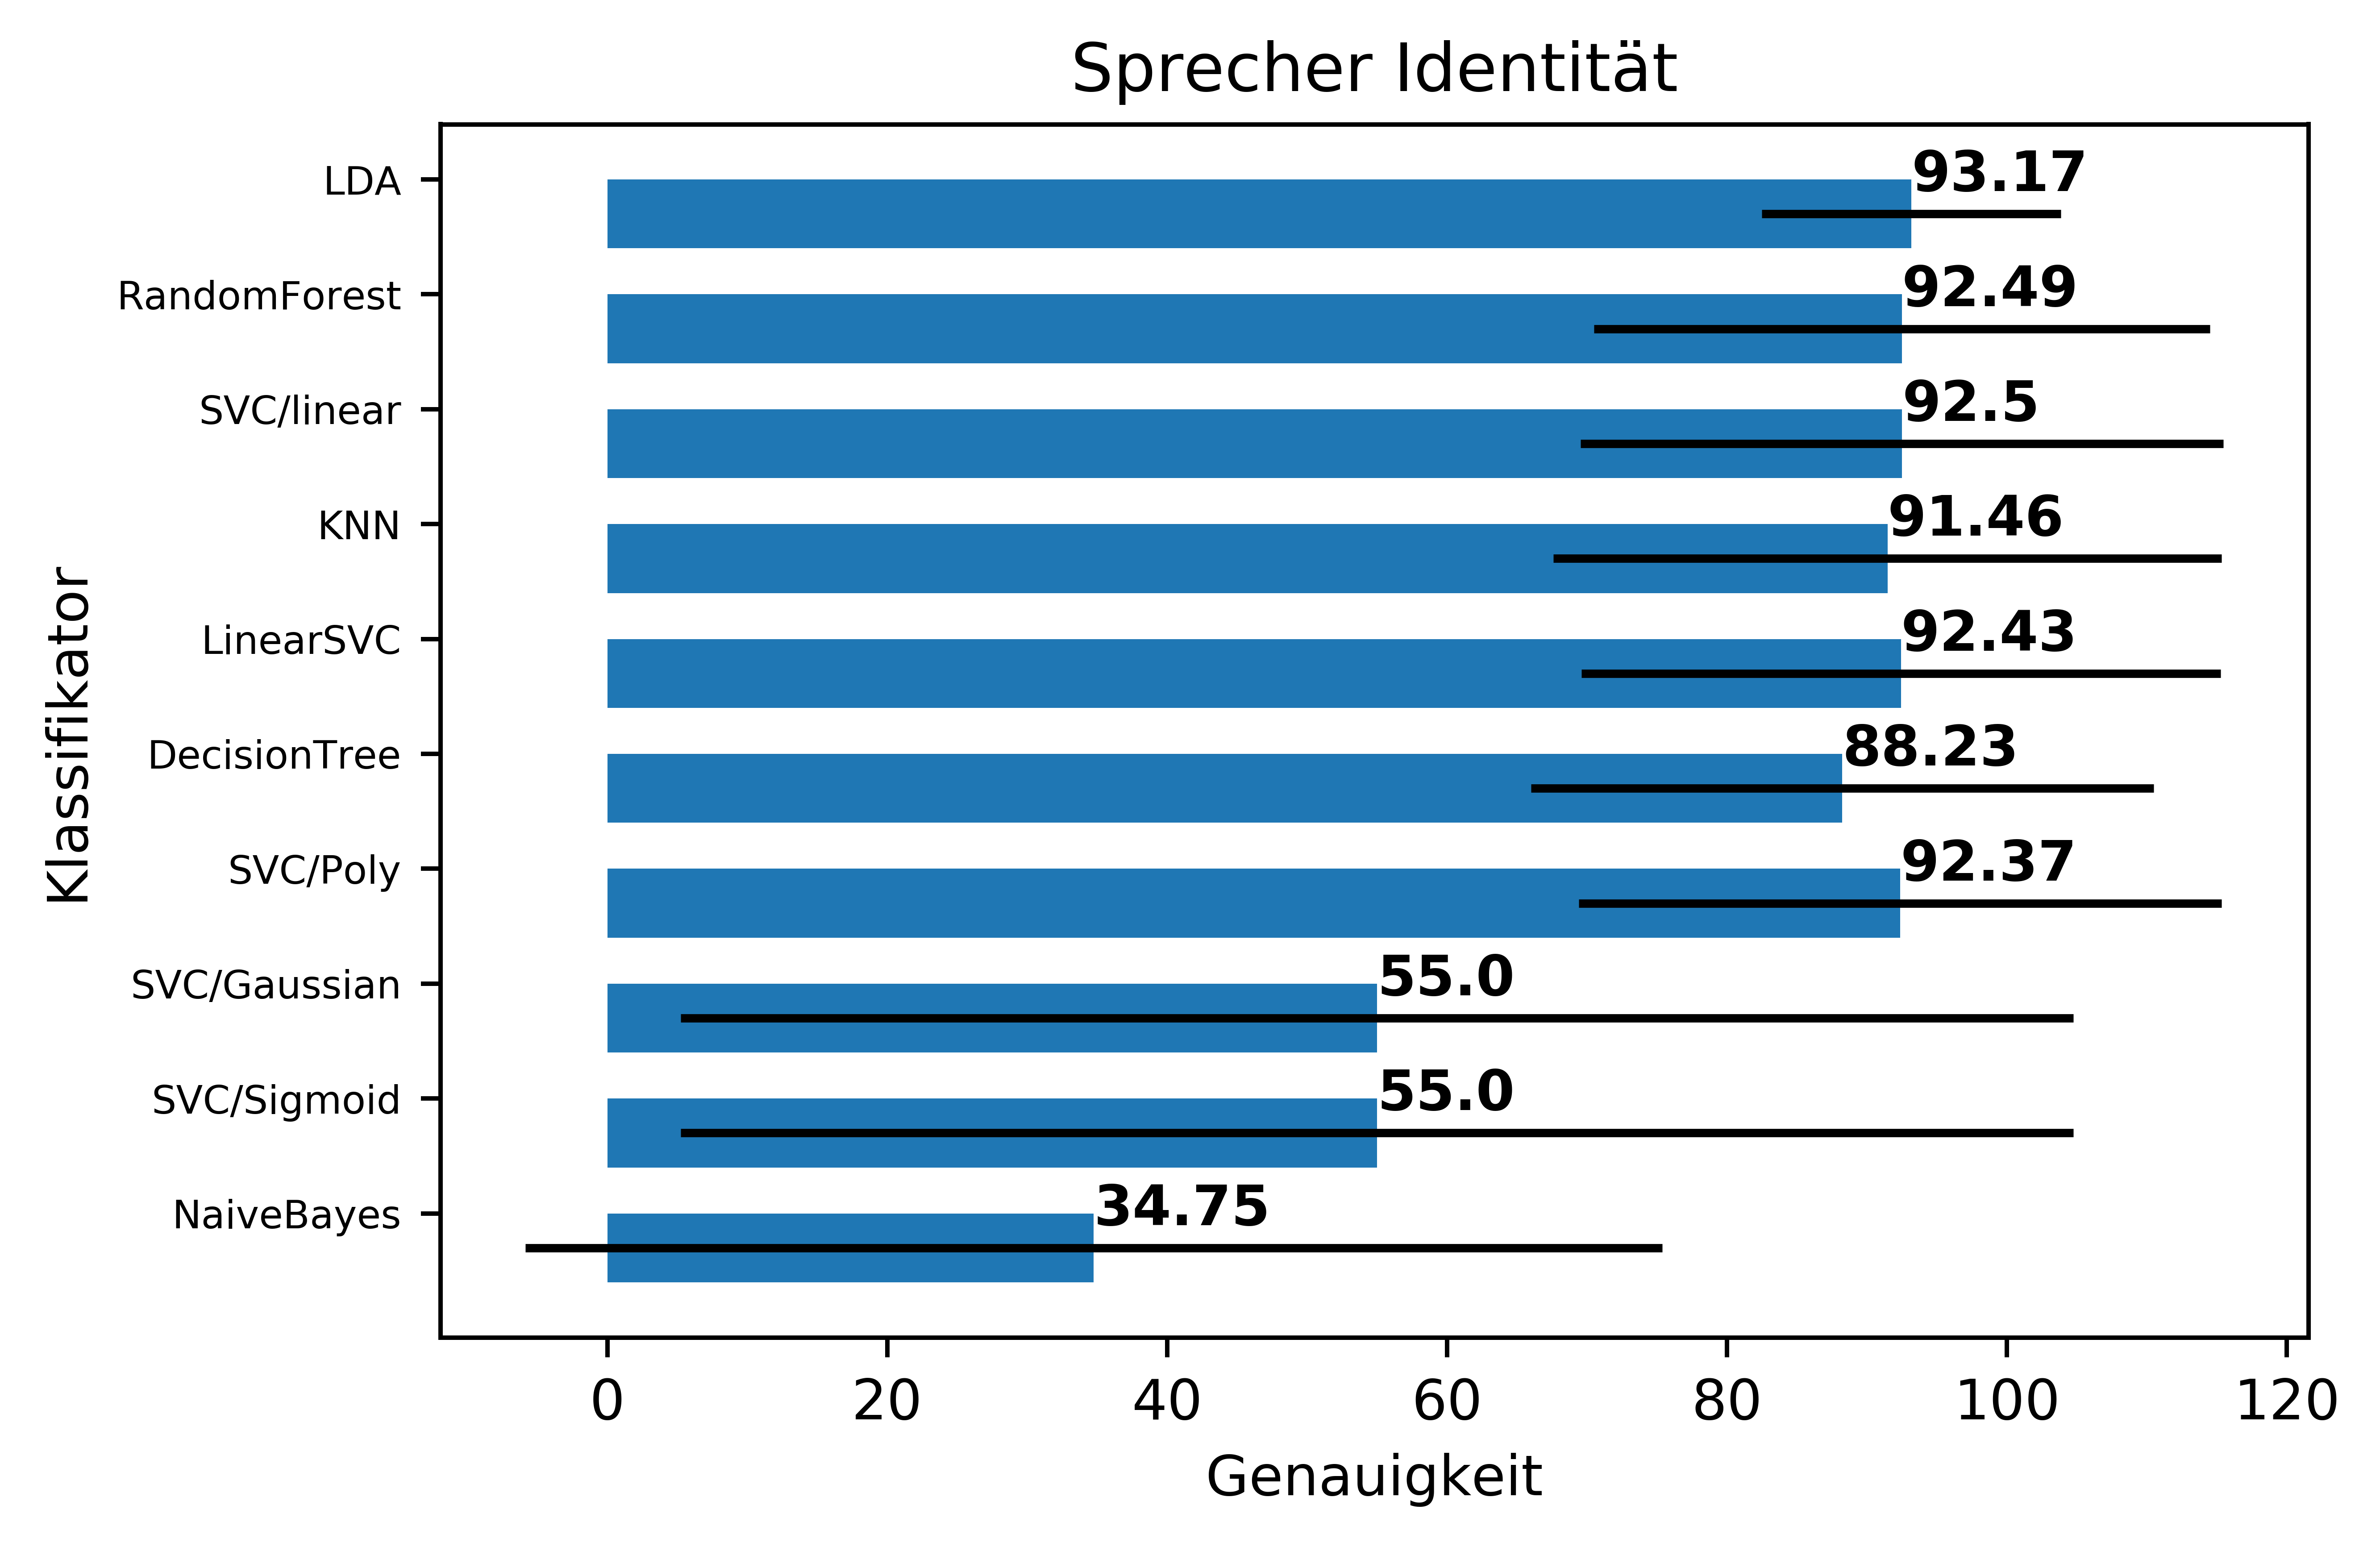
\includegraphics[width=70mm]{UserResults_unfiltered.png}}
\subfigure[Sprecher 2 und 8]{\label{fig:user2}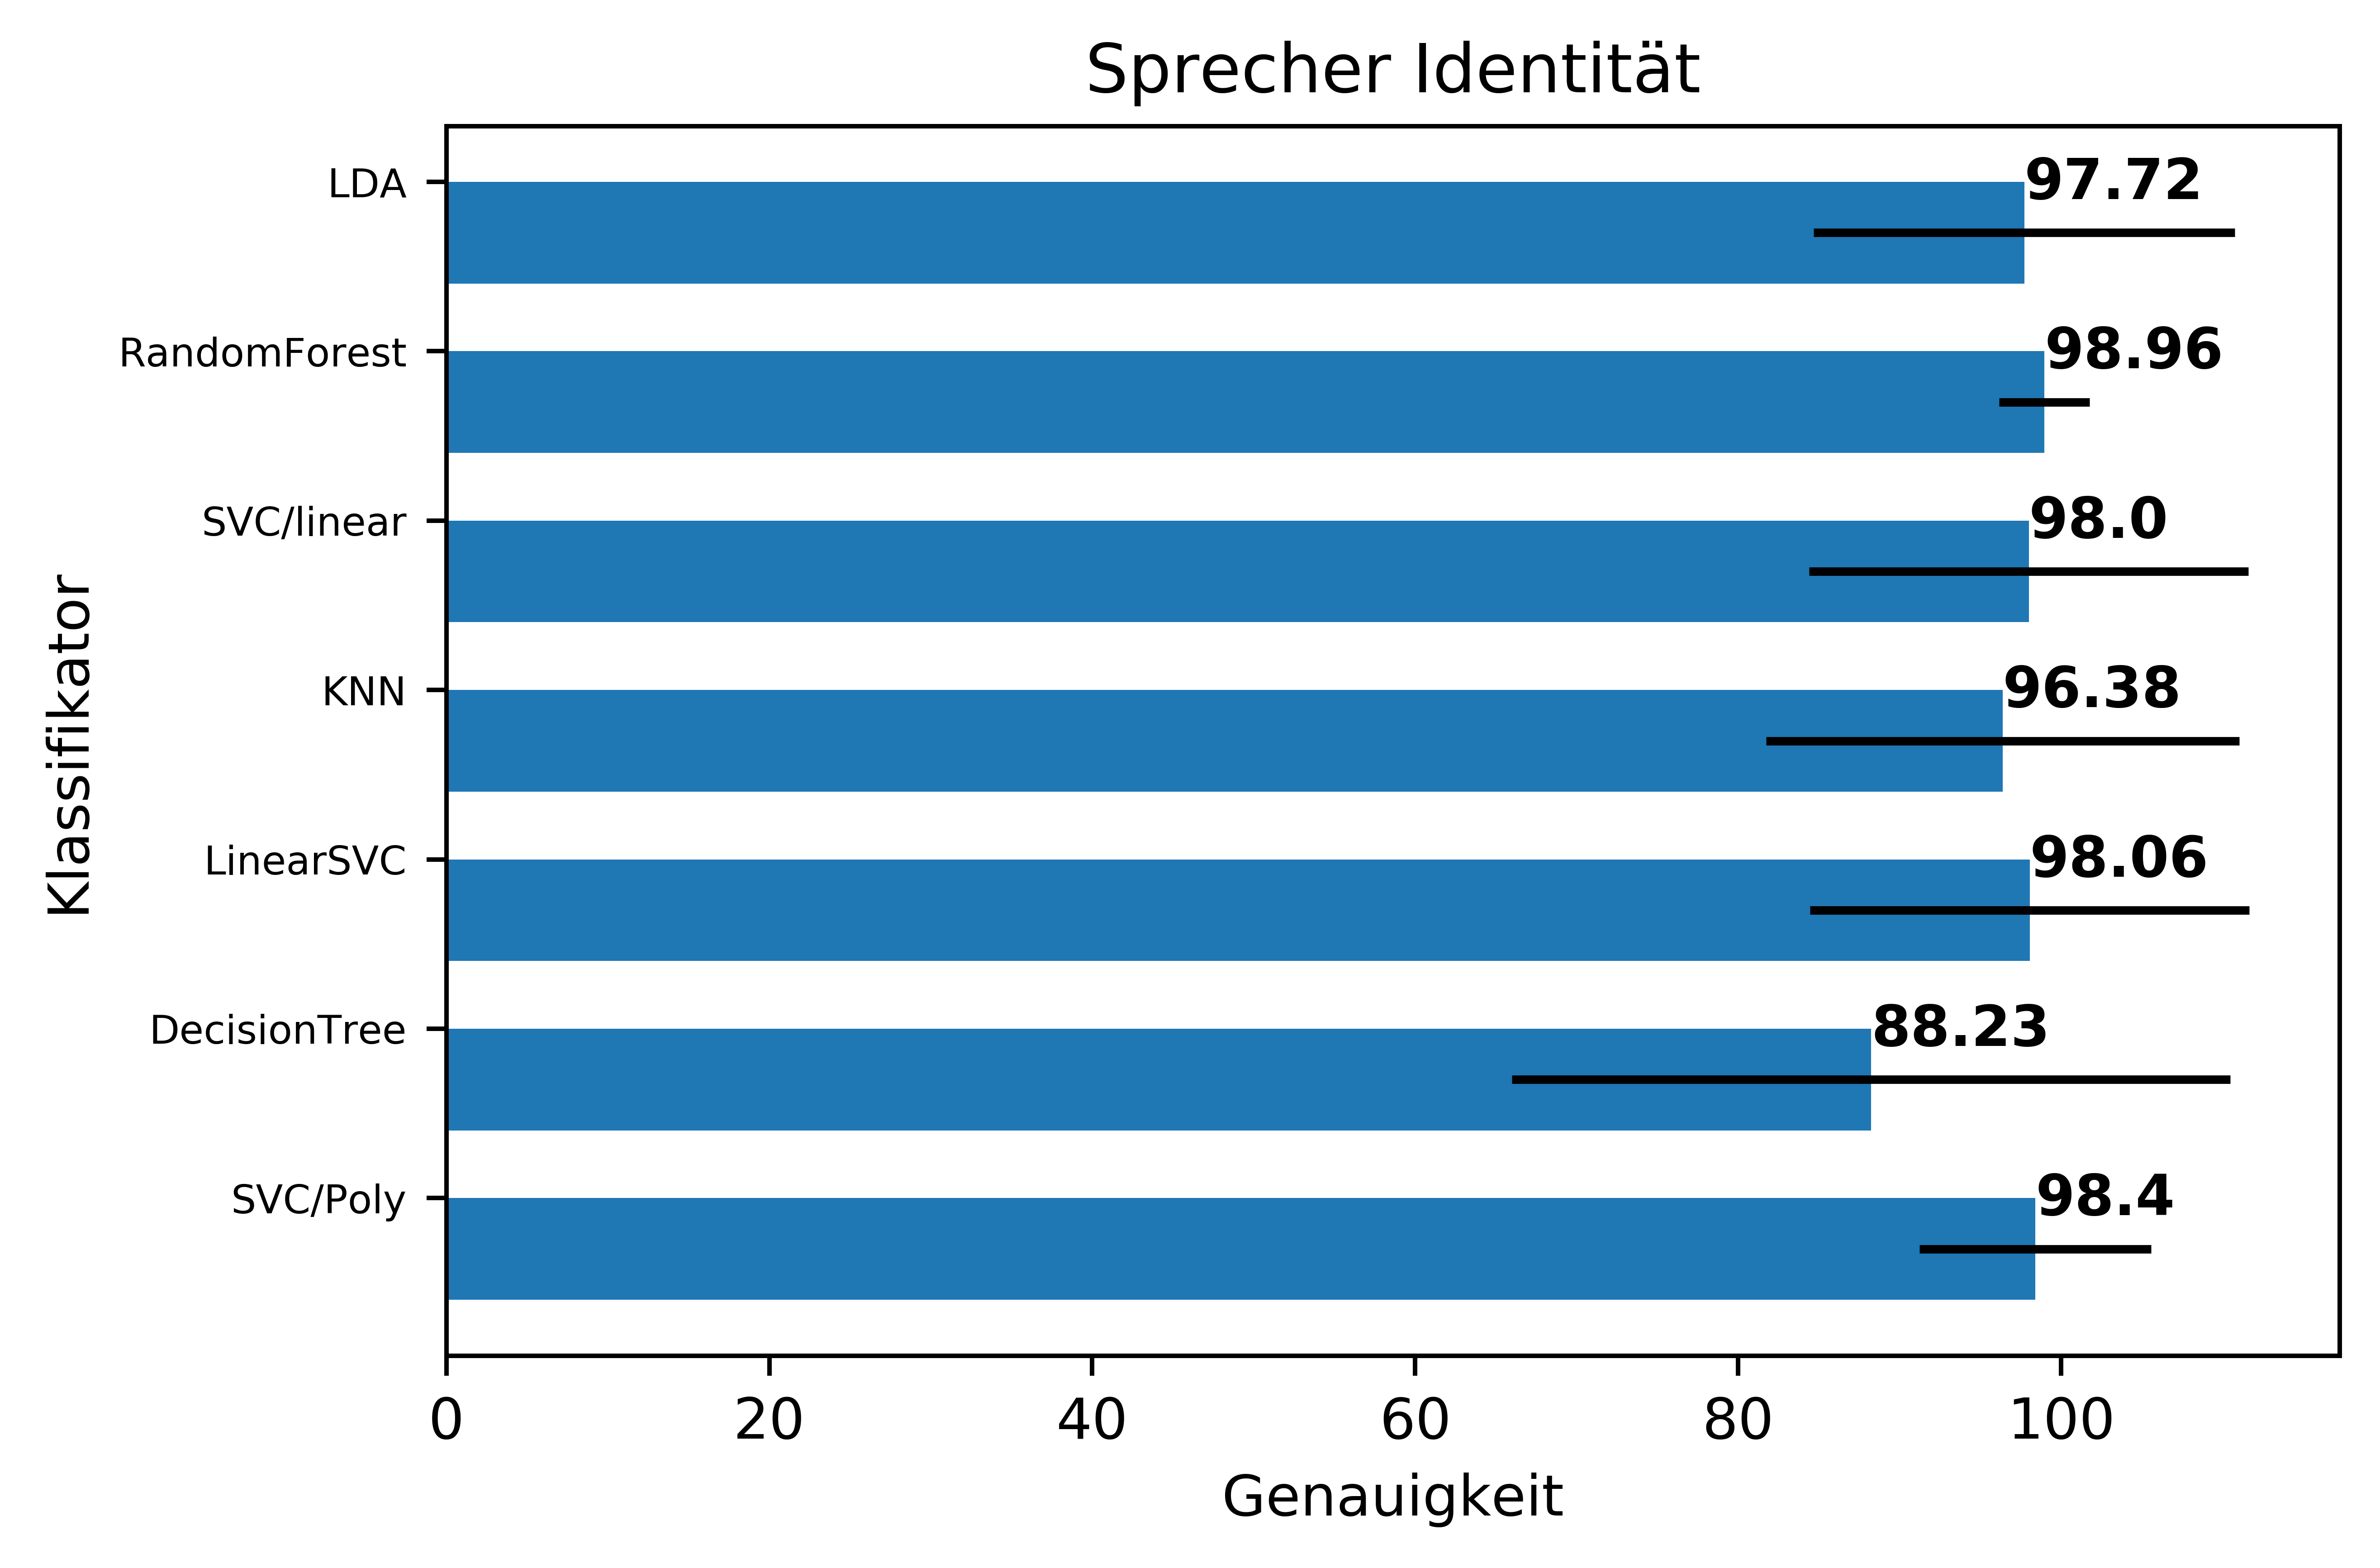
\includegraphics[width=70mm]{UserResultsUnfiltered2User.png}}
\caption{Durchschnittliche Genauigkeit, sowie die Standardabweichung der verschiedenen Klassifikatoren bei der Erkennung der Sprecheridentität.}
\label{fig:vergleich2}
\end{figure}

\begin{figure}[H]
  \centering
  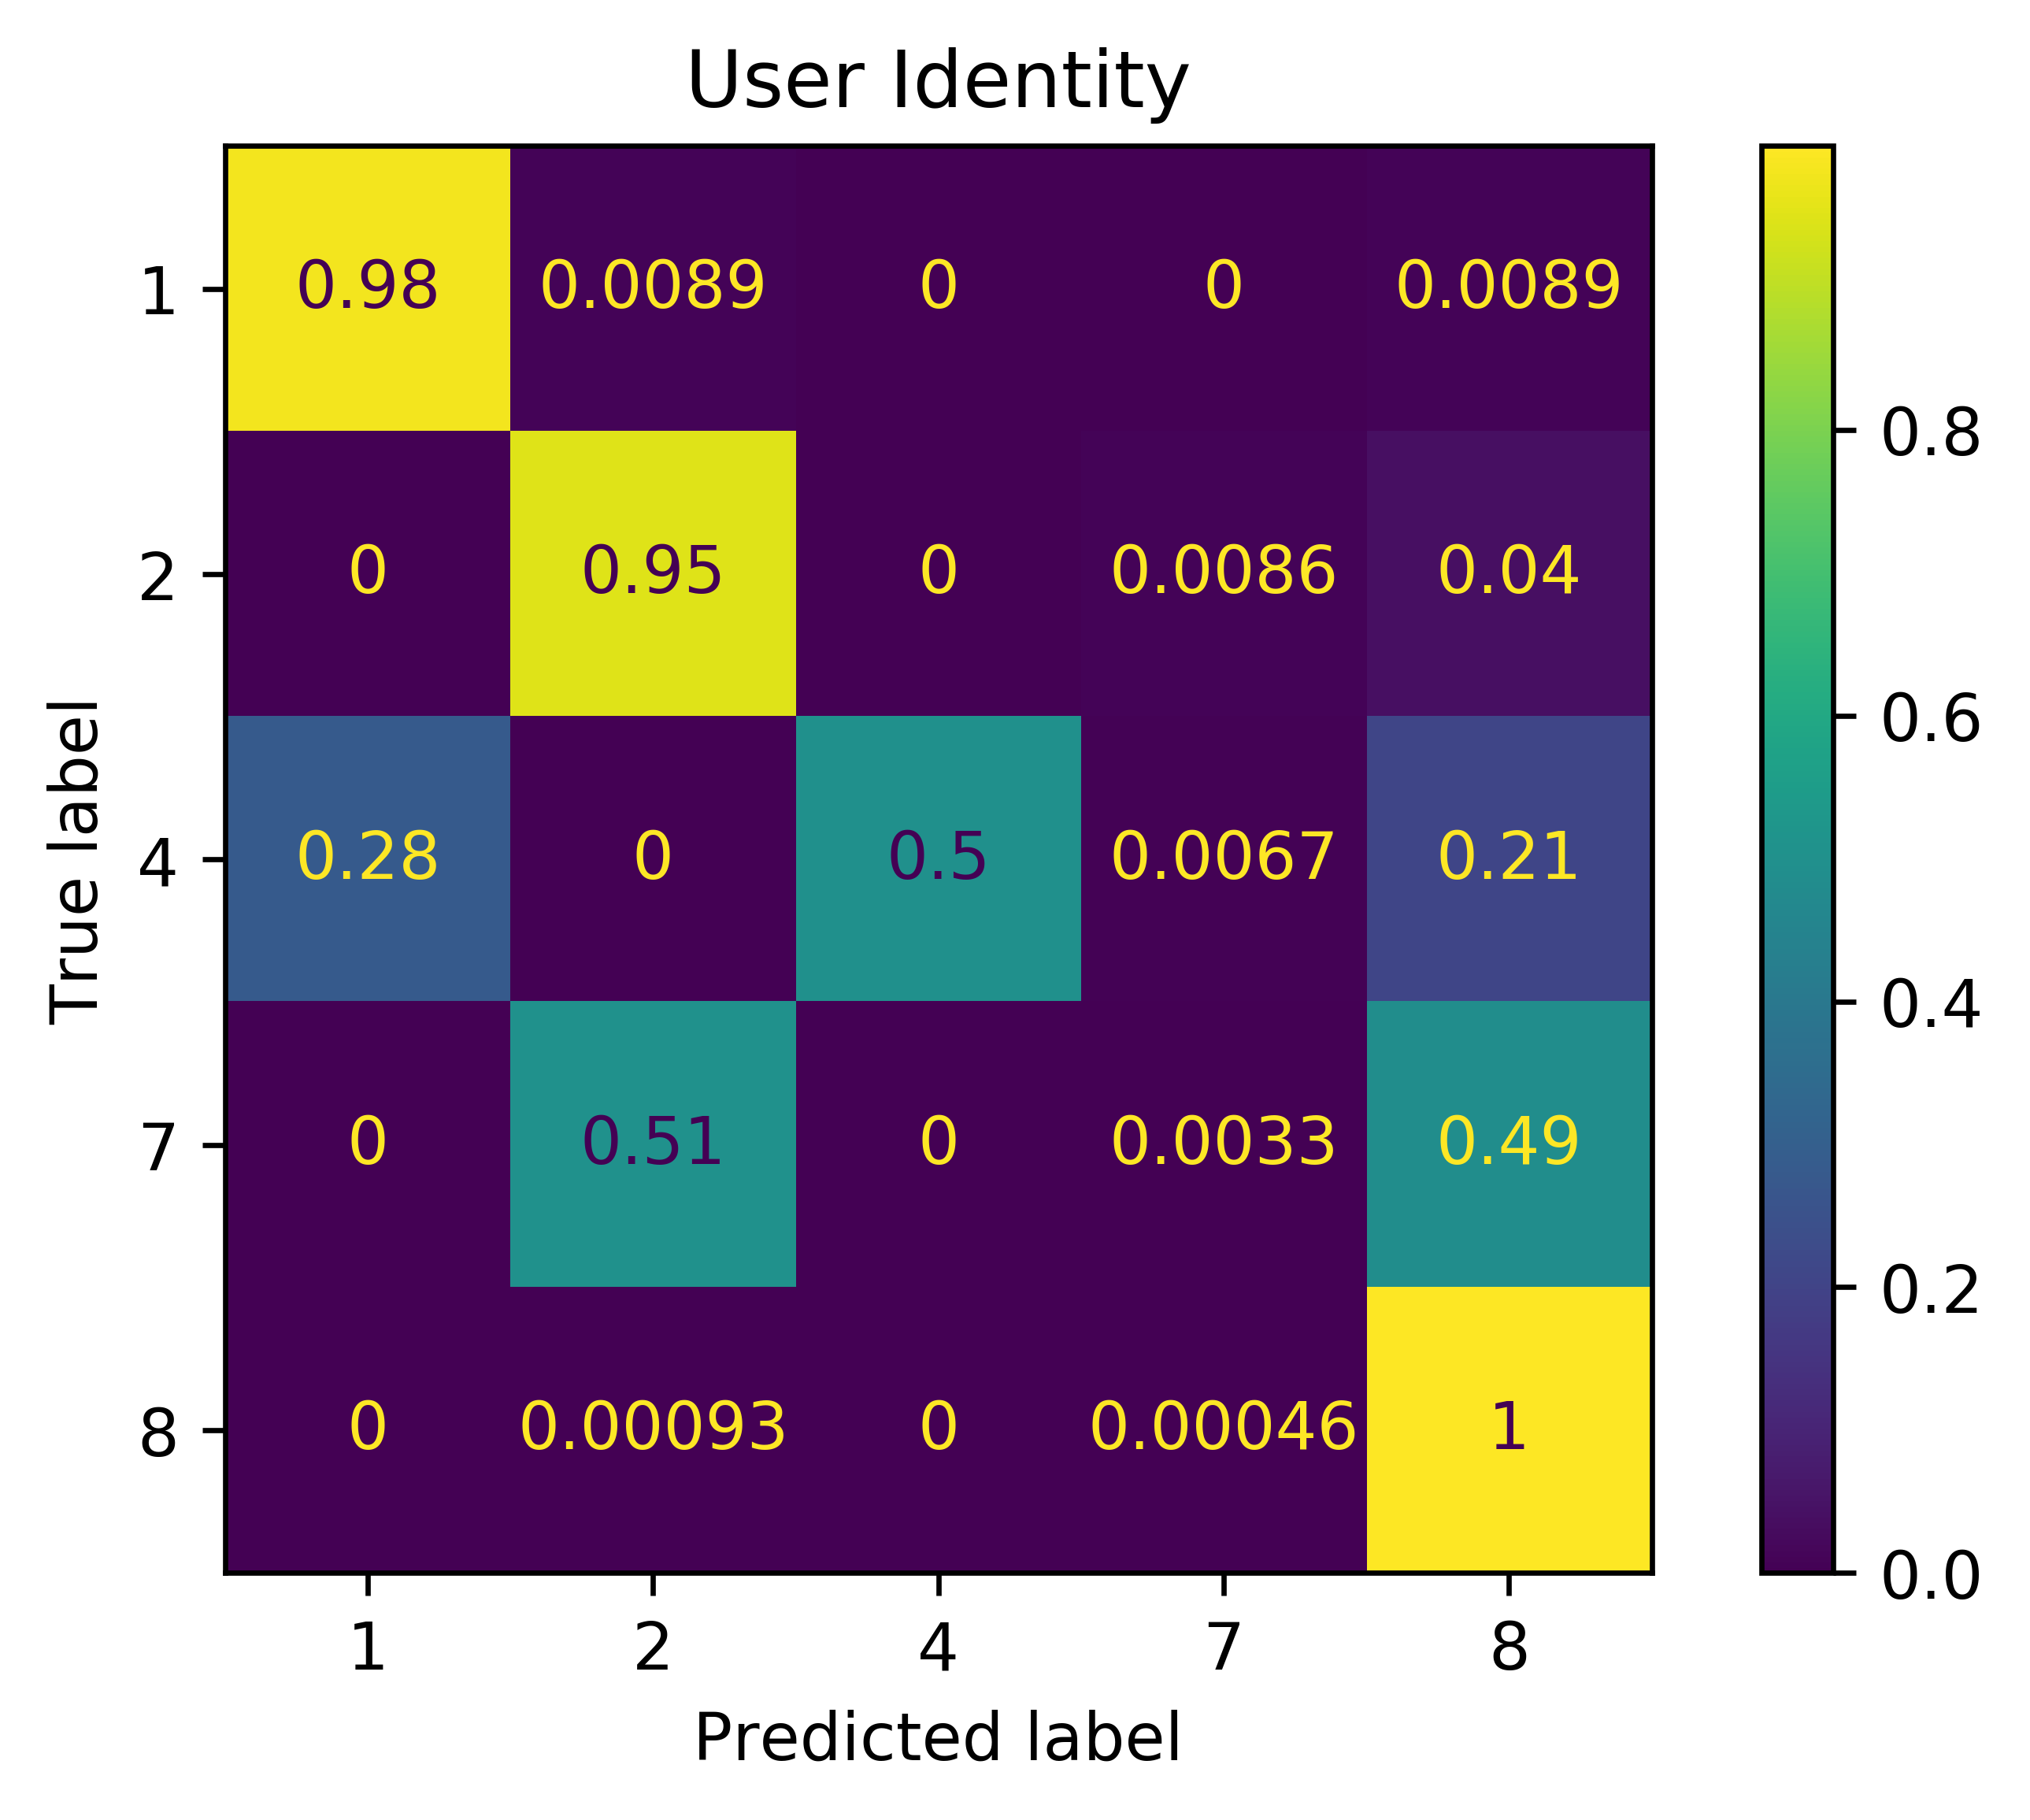
\includegraphics[width=100mm ,scale=0.6]{AllUserConfMatUnf.png}
  \caption{Confusion-Matrix der Erkennung der Sprecheridentität mit ungefilterten Daten.}
  \label{fig:Usercnf1}
\end{figure}

\subsubsection{Sessions}
Bei den Genauigkeiten der einzelnen Sessions sieht man, dass es eine ziemlich gleichmäßige Genauigkeit zwischen allen Sessions gibt. Die meisten Sessions von Sprecher 2 und 8 haben eine Genauigkeit von 100 Prozent deshalb wurde in der Tabelle \ref{tab:UnfSessions} die Sessions mit 100 prozentiger Genauigkeit entfernt. Es existieren jedoch einzelne Sessions die deutlich geringere Genauigkeiten aufweisen. In Sprecher 2 sieht man zum Beispiel in den Sessions 29 und 26 eine viel geringere Genauigkeit als bei allen anderen Sessions. In \ref{fig:cnf1} sieht man, dass in über 73 Prozent der Fälle Sprecher 2 mit Sprecher 8 verwechselt wird. In Session 26 sieht man, dass mit 32 Prozent ebenfalls eine hohe Verwechslung-rate mit Sprecher 8 vorhanden ist zudem ist in dieser Session noch eine 17 Prozent Verwechslung-rate mit Sprecher 7. Die restlichen Sessions von Sprecher 2 haben entweder eine Genauigkeit von 100 Prozent oder haben sehr wenige Verwechslungen mit dem anderen Sprechern.

\begin{table}[H]
 \centering
 \caption{Genauigkeiten aller Sessions bei der Sprecher Erkennung.}
\begin{tabular}{|c|c|}
\hline 
Session & Resultat in Prozent \\ 
\hline 
1001 & 96 \\ 
\hline 
1002 & 99,33 \\ 
\hline 
1003 & 99,33 \\ 
\hline 
2004 & 96,67 \\ 
\hline 
2008 & 99,33 \\ 
\hline 
2026 & 51 \\ 
\hline 
2027 & 93 \\ 
\hline 
2029 & 26,67 \\ 
\hline 
2031 & 96 \\ 
\hline 
4001 & 100 \\ 
\hline 
4002 & 0 \\ 
\hline 
7001 & 0,7 \\ 
\hline 
7002 & 0 \\ 
\hline 
8005 & 98 \\ 
\hline 
8014 & 98 \\ 
\hline
\label{tab:UnfSessions} 
\end{tabular} 
\end{table}
  

\begin{figure}[H]
  \centering
  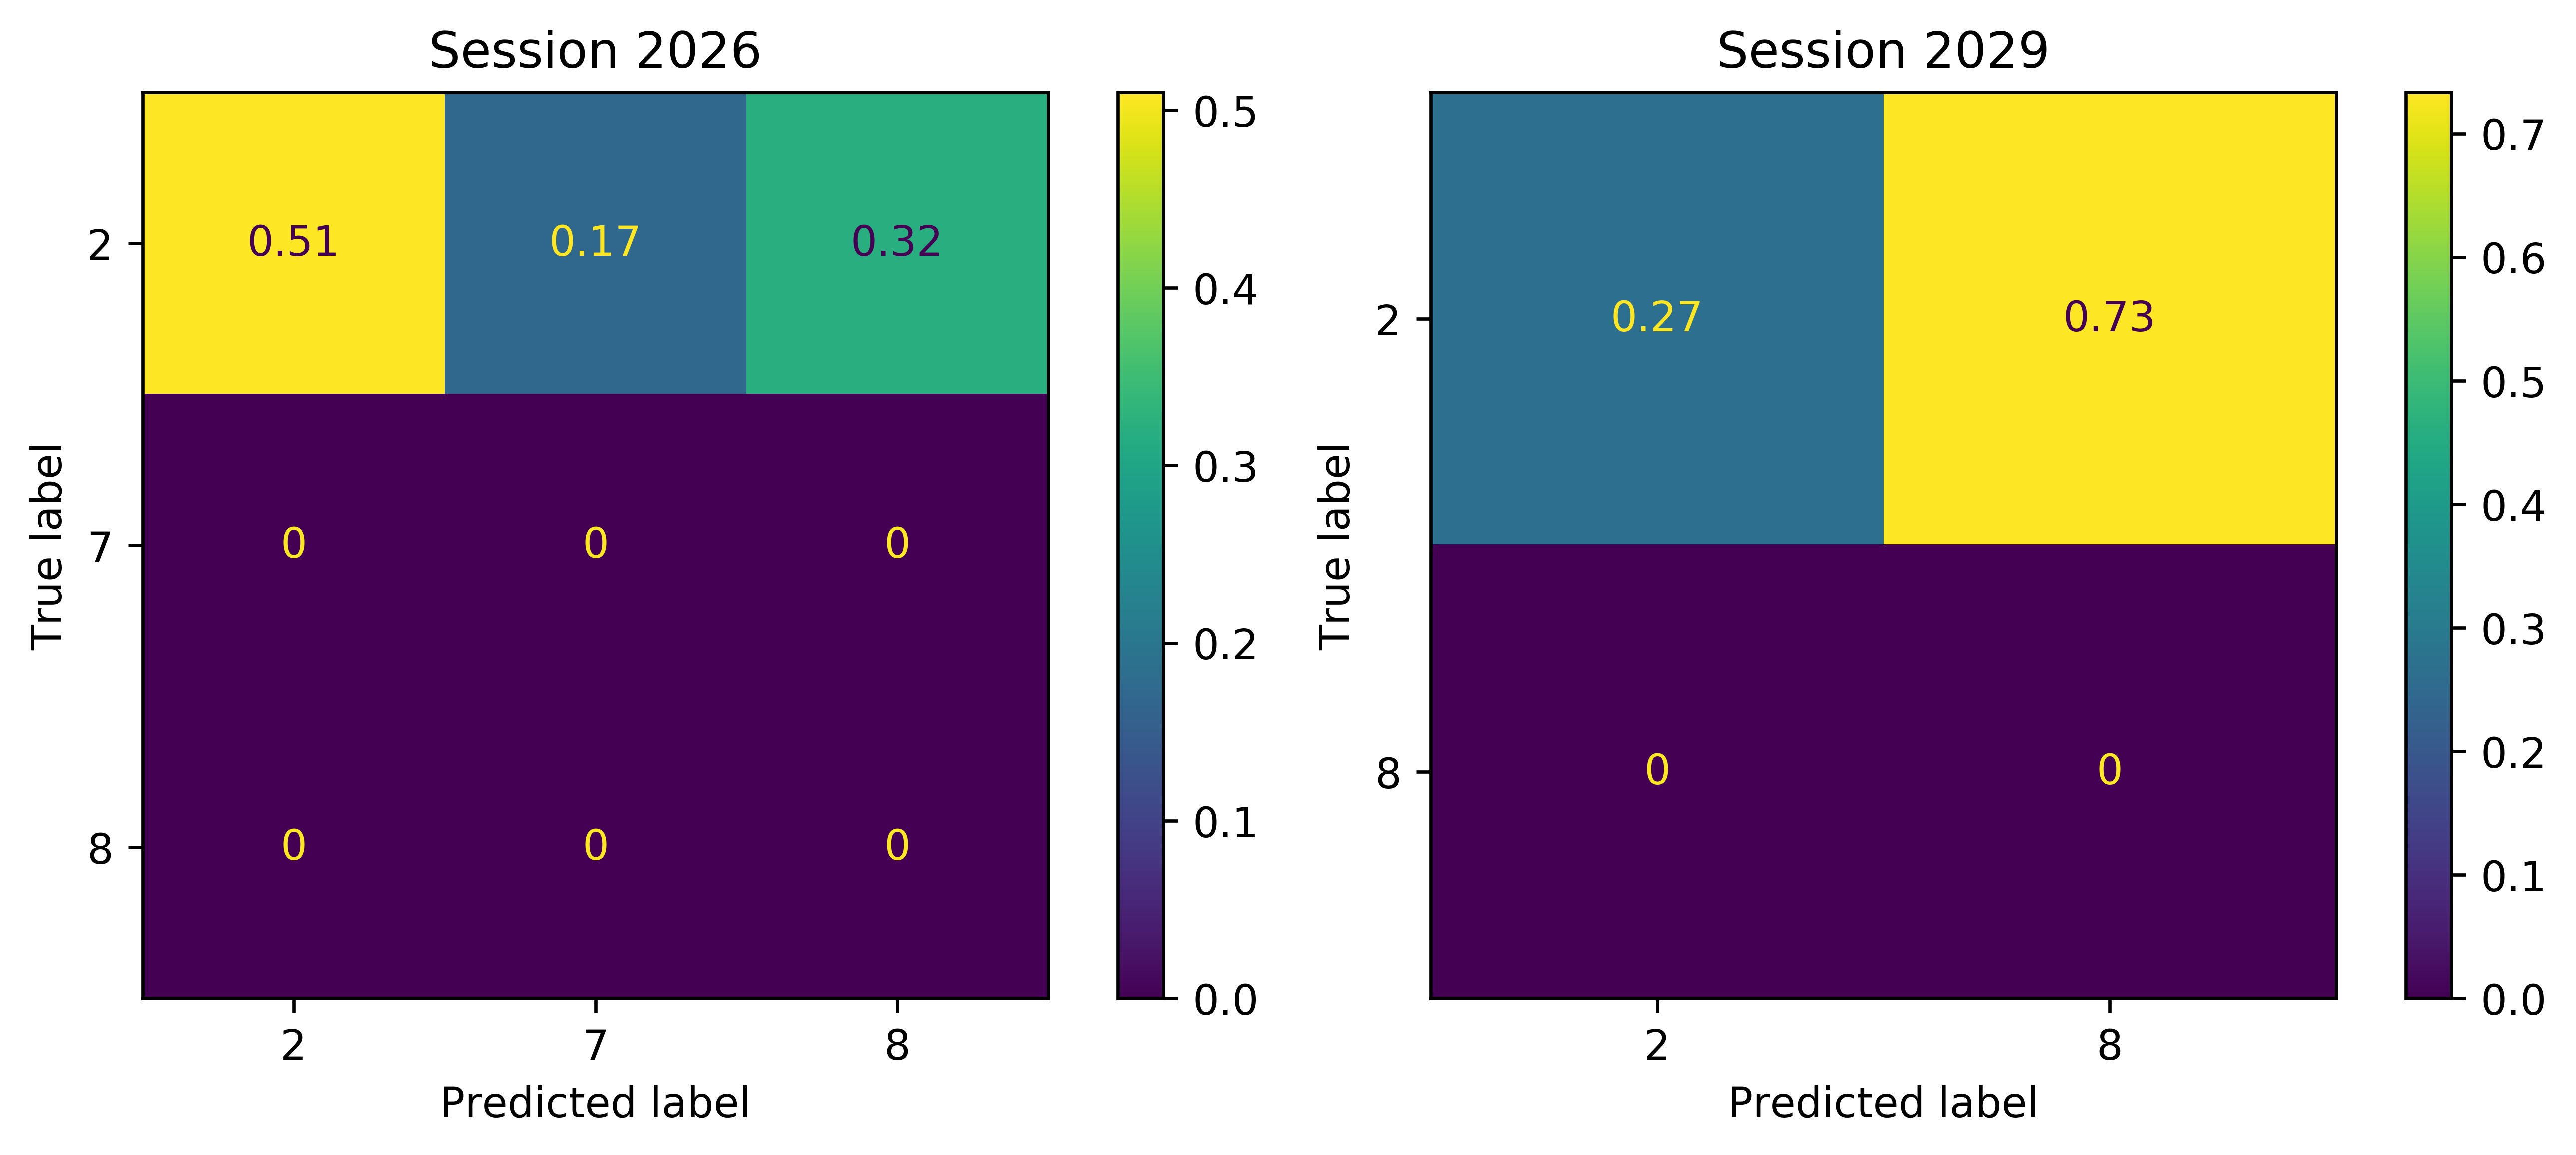
\includegraphics[width=100mm ,scale=0.6]{UserConfMatUser2Unf.png}
  \caption{Confusion-Matrix der Session 29 und 26 von Sprecher 2}
  \label{fig:cnf1}
\end{figure}

Bei Sprecher 8 mit einer vergleichbaren Anzahl an Sessions sind solche Ausnahmen nicht zu sehen.
Bei Sprecher 4 in Session 2 und in beiden Sessions von Sprecher 7 sieht man eine weit niedrigere Genauigkeit als in den Sessions der anderen Sprecher. Für Sprecher 4 ist die Genauigkeit bei der zweiten Session 0 Prozent und bei der ersten Session sehr hoch (\ref{tab:UnfSessions}). In \ref{fig:cnf2} sieht man wie sich die Genauigkeit von 0 in dieser Session ergibt. Sprecher 4 wird hier zu 57 Prozent mit Sprecher 1 und zu 42 Prozent mit Sprecher 8 verwechselt.

\begin{figure}[H]
  \centering
  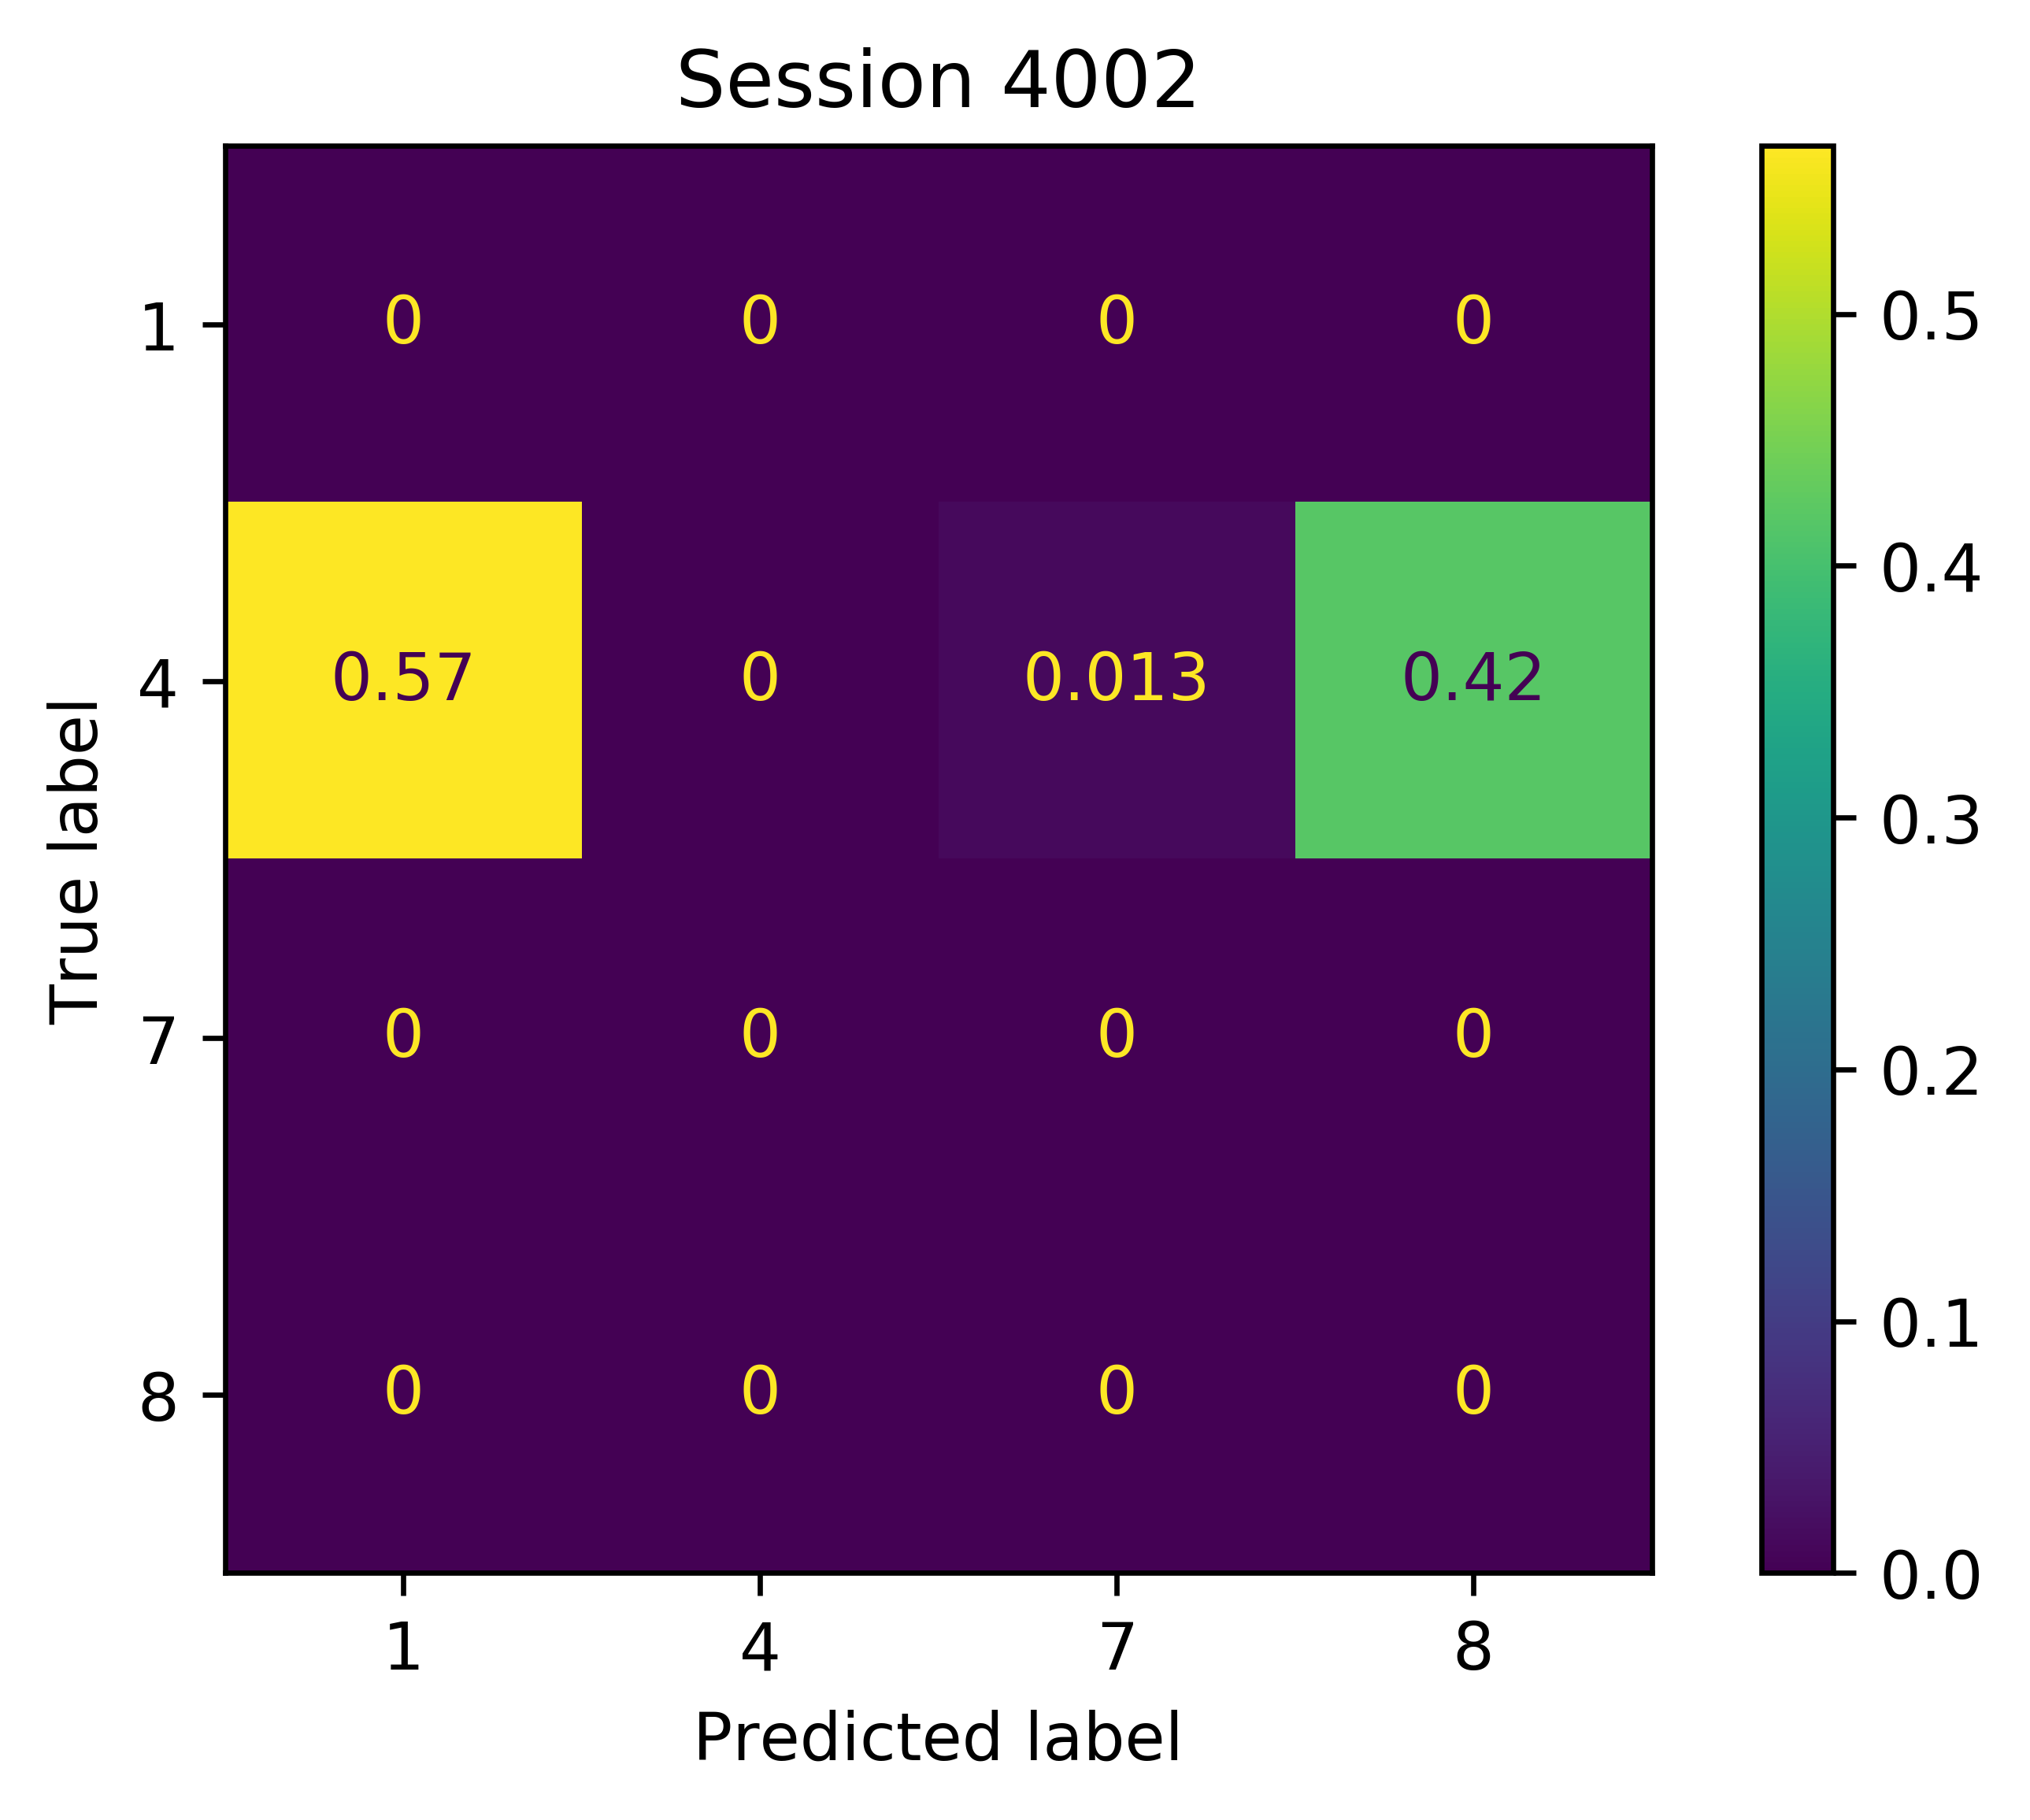
\includegraphics[width=80mm ,scale=0.6]{userCrossSessionUnf/Session 4002Unf.png}
  \caption{Confusion-Matrix der Session 2 von Sprecher 4}
  \label{fig:cnf2}
\end{figure}

Ich vermute, dass es nicht nur auf die Anzahl der Sessions, sondern auch auf die Qualität der Sessions ankommt, denn bei Sprecher 4 kann man einen großen Unterschied zwischen der ersten und der zweiten Session sehen. Zudem hat Sprecher 7 eine niedrigere Genauigkeit in beiden Sessions, also scheint die Anzahl an Sessions alleine auch eine Rolle zu spielen. In \ref{fig:cnf3} sieht man, warum die Genauigkeit von Sprecher 7 so niedrig ist. In Sprecher 7 werden nur die Sprecher mit den meisten Sprechern, also 2 und 8, vorhergesagt.

\begin{figure}[H]
  \centering
  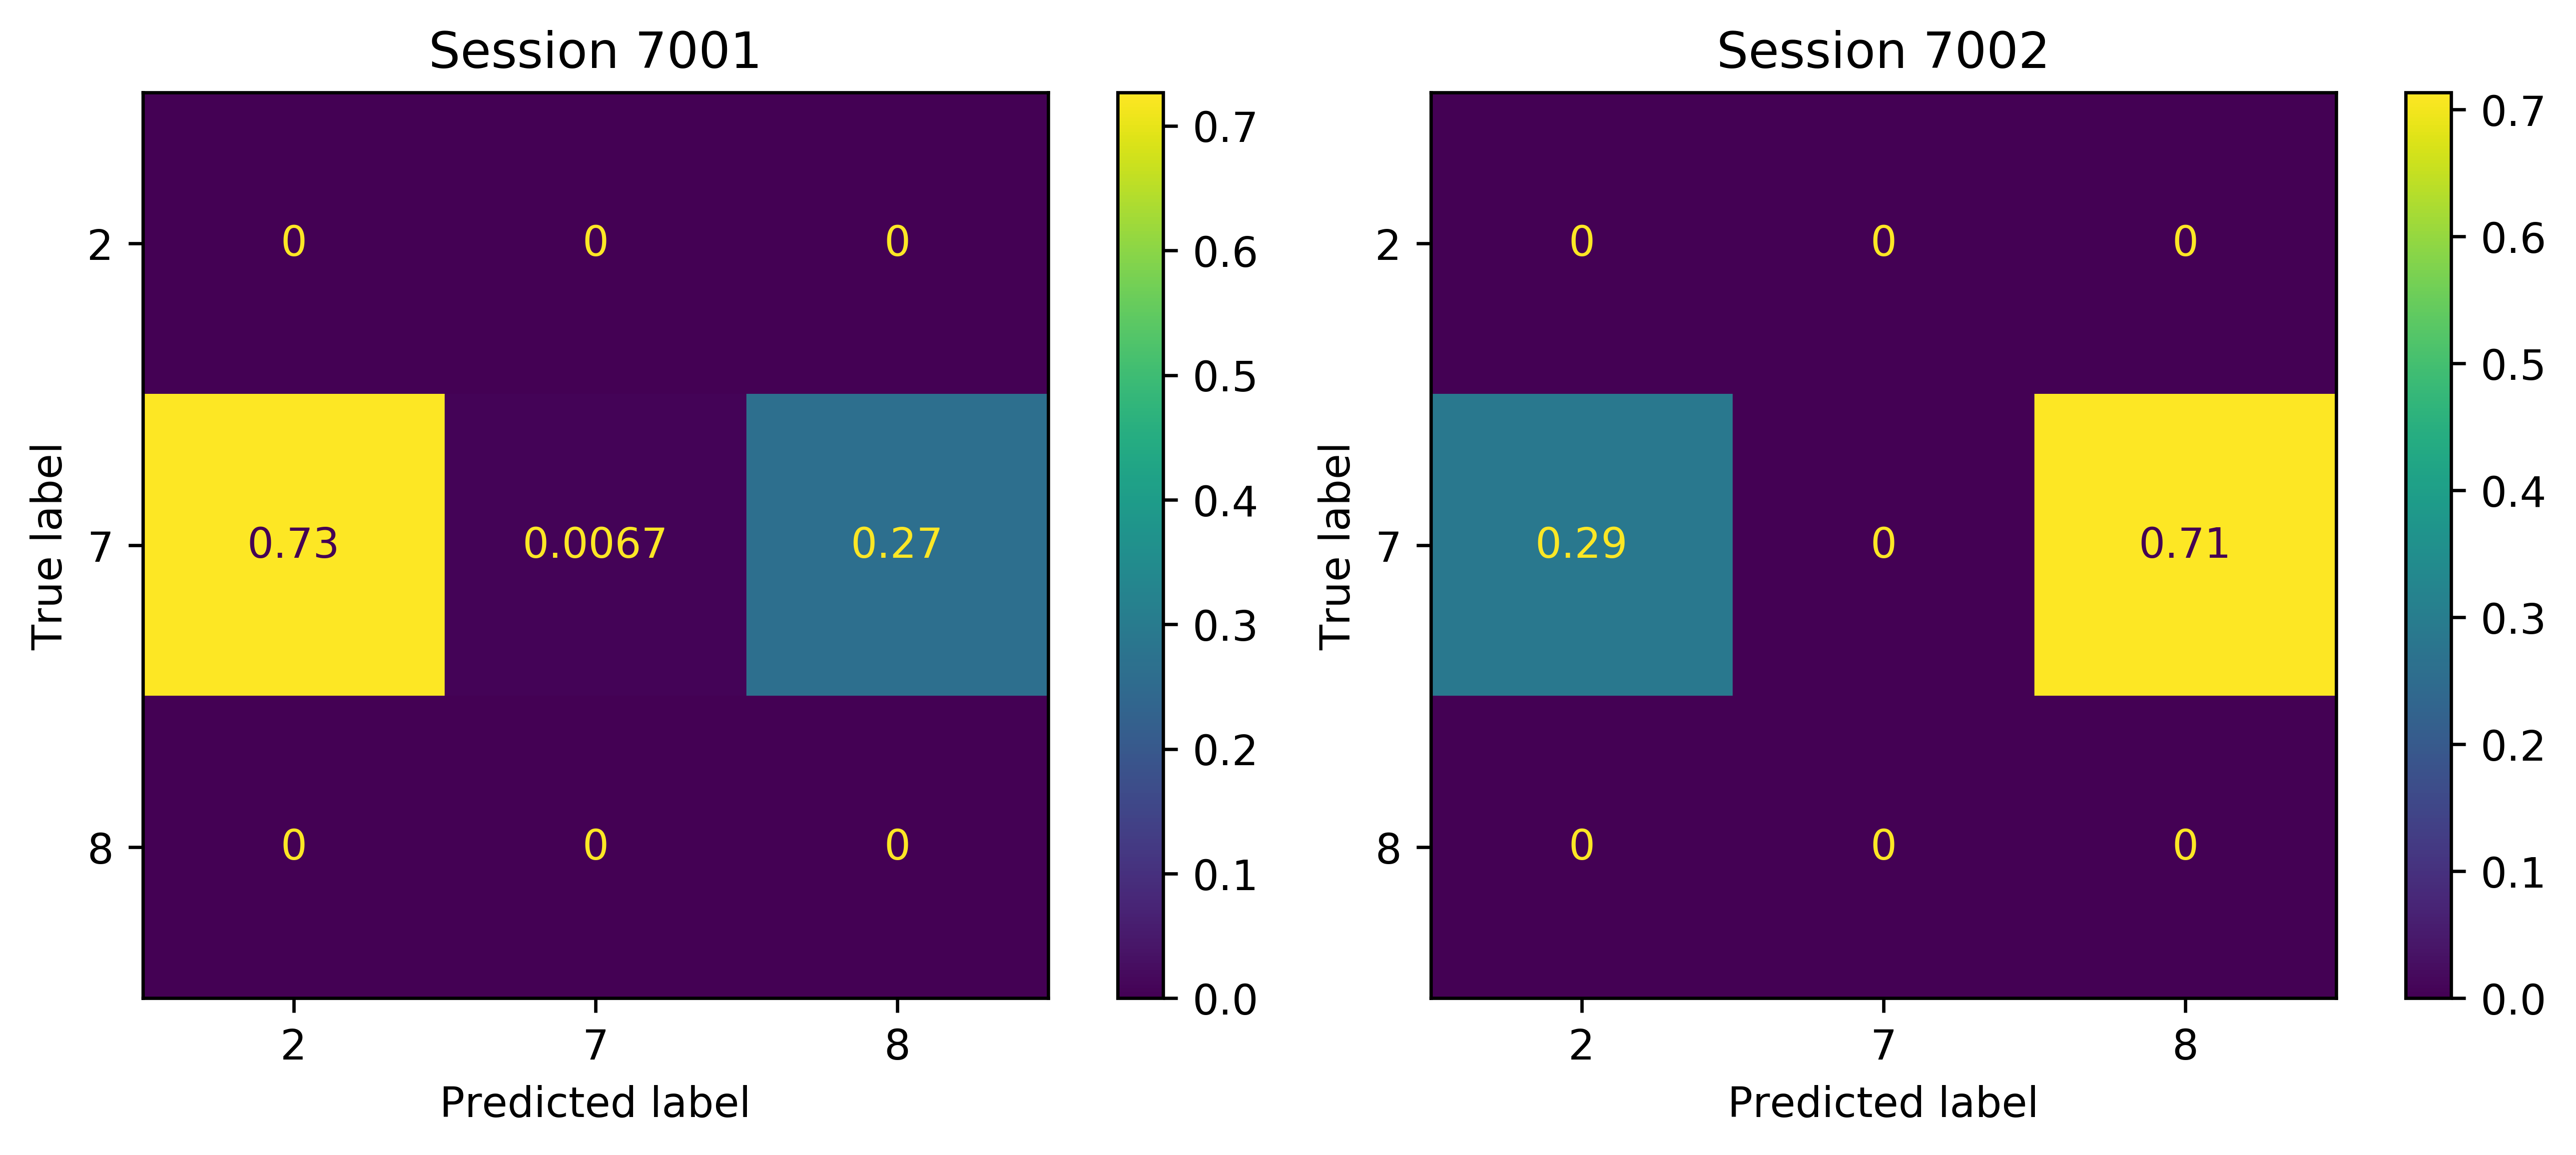
\includegraphics[width=100mm ,scale=0.6]{UserConfMatUser7Unf.png}
  \caption{Confusion-Matrix der beiden Sessions von Sprecher 7}
  \label{fig:cnf3}
\end{figure}

 
Die Sprecher mit den meisten Sessions haben nämlich eine sehr hohe Genauigkeit (siehe Sprecher 2 und 8). Jedoch ist in Sprecher 1 die Genauigkeit mit über 95 Prozent für jede Session, trotz weniger Daten sehr hoch wodurch ich mehr auf die Qualität der Sessions als Hauptmerkmal tendiere.
Bei diesen Tests viel auf, dass die Genauigkeit für die Sprecher mit weniger Daten vergleichbar viel niedriger sein kann  als die Genauigkeit für die anderen Sprecher. Deshalb habe wurde ein zweiter Versuch durchgeführt in dem nur die Daten der Sprecher 2 und 8 beobachtet wurde. Dabei waren die Resultate deutlich besser als in dem vorherigen versuch (siehe  \ref{fig:user2}). Um den Effekt der Sessionqualität auf die Genauigkeit zu bestimmen wurden im späteren Verlauf die Sessions mit einer niedrigen Genauigkeit entfernt und es wurde erneut getestet. 


\paragraph{Session 29 entfernt} 
Man sieht in \ref{fig:Usercnf1_without29} das die Erkennungsrate für Sprecher 2 um 3 Prozent von 95 auf 98 Prozent steigt. Für Sprecher 7 steigt die Verwechslung-rate mit Sprecher 2 um 5 Prozent von 51 zu 56 Prozent. Ich gehe davon aus das es steigt, weil Sprecher 2 jetzt einen gleichmäßigeren Datensatz besitzt. Die anderen Sprecher bleiben gleich.

Die Ergebnisse sowie der Vergleich zu der Version mit Session 29 ist in der Tabelle \ref{tab:UnfSessionsNo29} zu sehen. Es werden die vorherigen Ergebnisse mit den neuen verglichen und in der letzten Zeile gezeigt wie es sich geändert hat.

\paragraph{}
In den vorherigen Tests ist aufgefallen, dass Session 29 beim Sprecher 2 eine viel niedrigere Genauigkeit aufweist als die anderen Sessions desselben Sprechers. Aus diesem Grund wurde hier ein weiterer Test durchgeführt in dem Session 29 aus Sprecher 2 entfernt wurde. Bei den Ergebnissen dieses Versuches ist eine Steigerung der Genauigkeit, in Session 26 von Sprecher 2 von 51 auf 58 Prozent zu beobachten. Genauer kann man in \ref{fig:cn4} sehen das die Verbesserung der Genauigkeit auf die verringerte Anzahl der Verwechslungen von Sprecher 2 und Sprecher 8 zurückzuführen ist. Gleichzeitig ist aber auch ein Fall der Genauigkeit in den Sessions 27 und 31 zu sehen. Die niedrigere Genauigkeit liegt an der höheren Verwechslung-rate von Sprecher 2 mit Sprecher 7 (\ref{fig:2027unfNo2029} und \ref{fig:2031unfNo2029}) in Sprecher 1 kann man eine leichte Entwicklung der Genauigkeiten ins Negative in \ref{fig:cnf2} kann man sehen das Sprecher 2 am häufigsten mit Sprecher 1 verwechselt wird. Den ersten beiden Sessions beobachten (\ref{tab:UnfSessionsNo29}). Bei Sprecher 4 ist wiederum ein leichter Fall der Genauigkeit für die erste Session von 100 Prozent auf 99.33 Prozent zu sehen(\ref{tab:UnfSessionsNo29}) die zweite Session bleibt jedoch bei 0, ich gehe davon aus das bei dieser Session ein Fehler bei der Aufnahme passiert ist. Die Genauigkeit bei Sprecher 7 ändert sich nicht.

\begin{figure}[H]
  \centering
  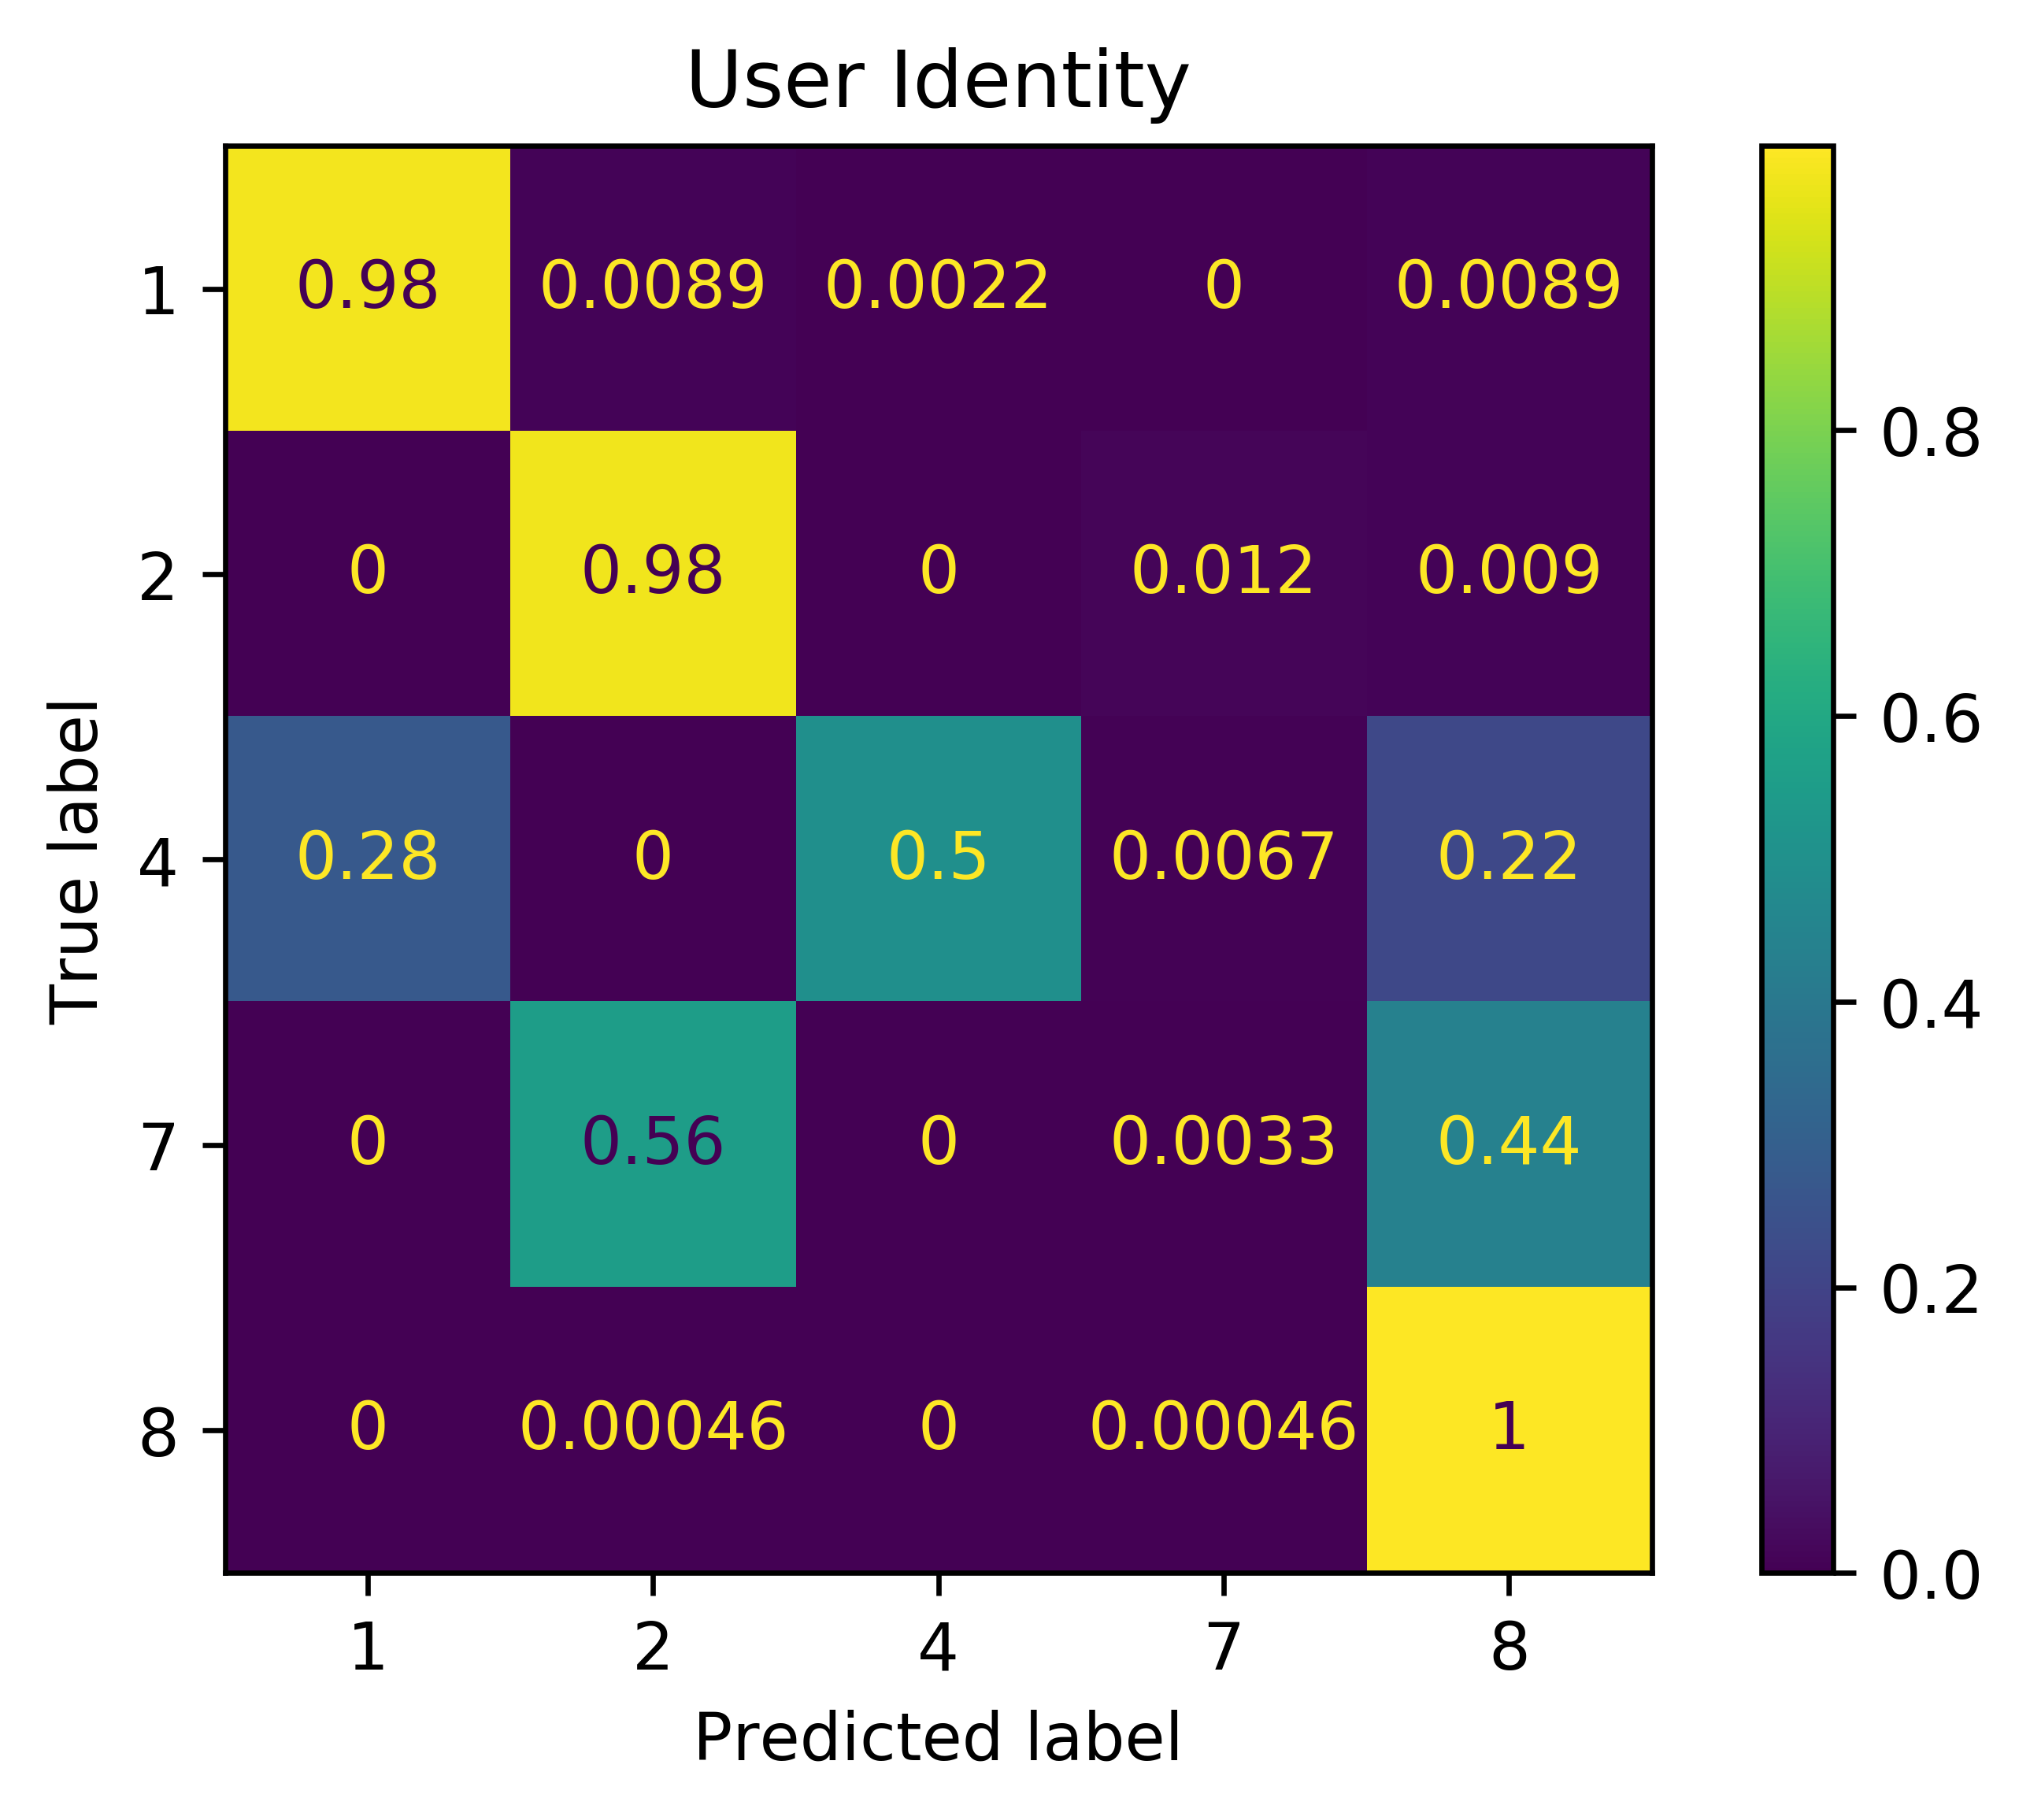
\includegraphics[width=100mm ,scale=0.6]{AllUserConfMatUnf_without29.png}
  \caption{Confusion-Matrix der Erkennung Sprecheridentität mit ungefilterten Daten.}
  \label{fig:Usercnf1_without29}
\end{figure}

\begin{figure}[H]
  \centering
  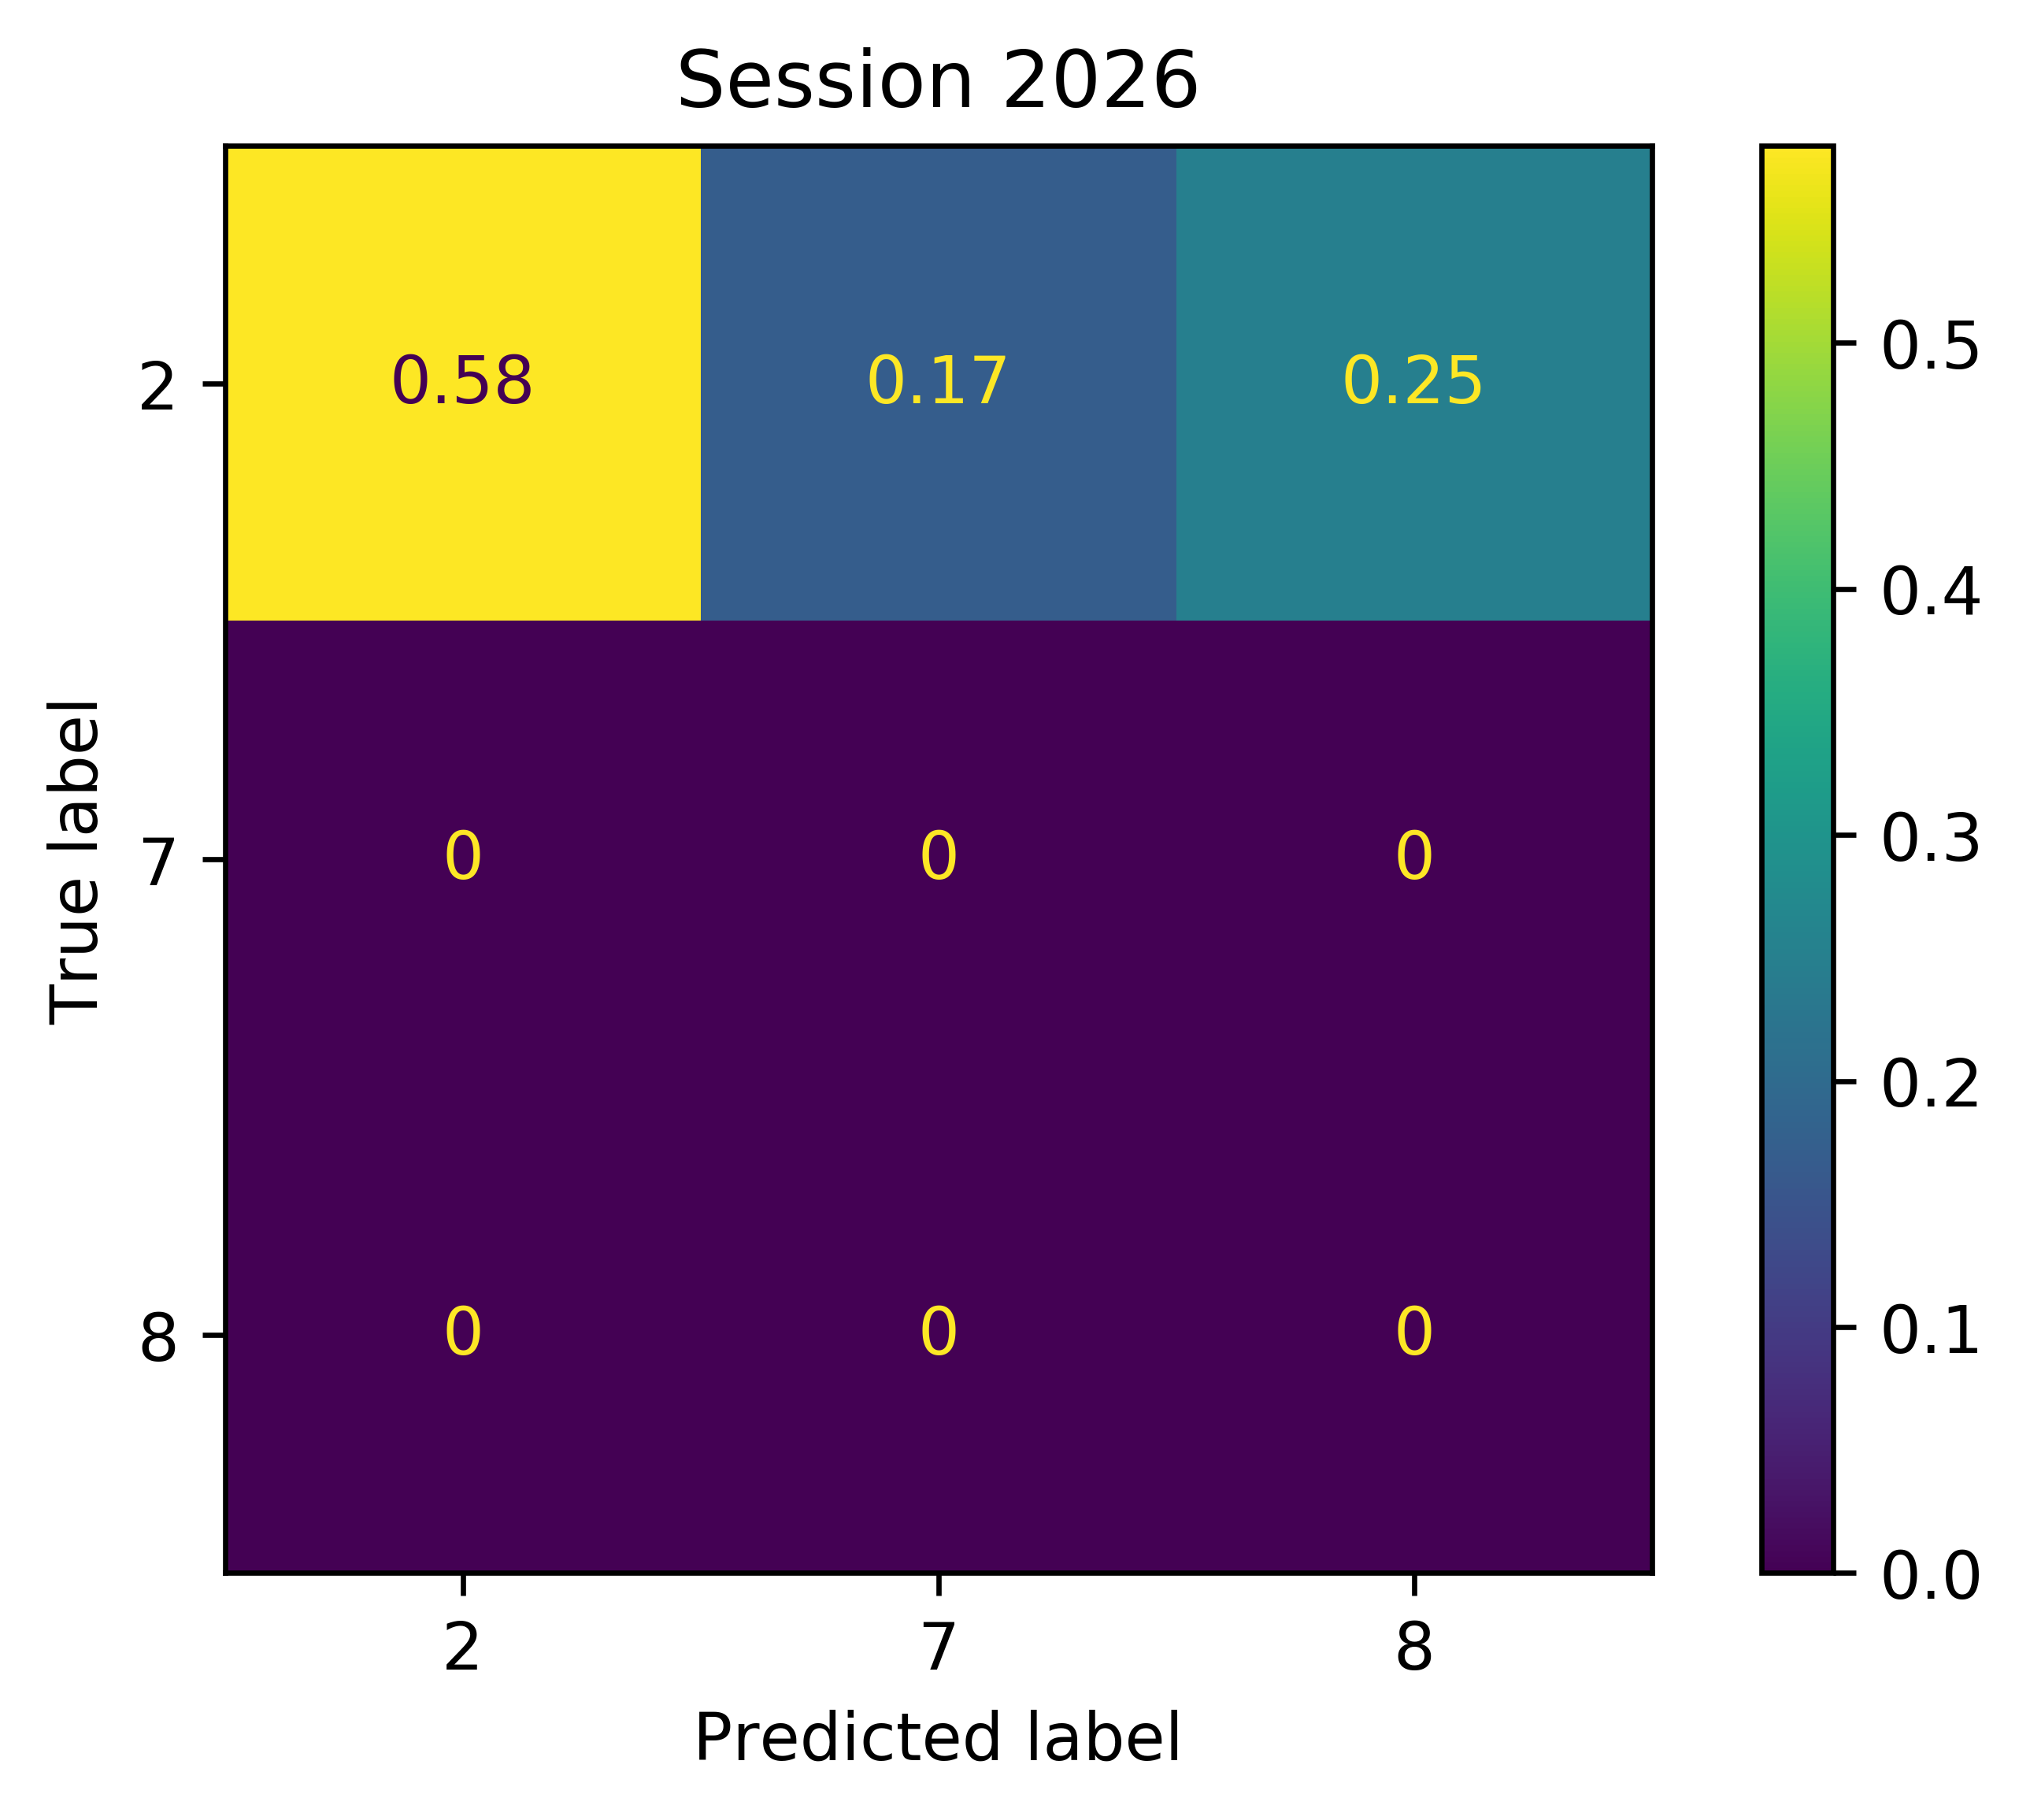
\includegraphics[width=80mm ,scale=0.6]{userCrossSessionUnf_without29/Session 2026Unf_without29.png}
  \caption{Erkennungsraten verschiedener Sprecher bei der Klassifizierung der Sprecheridentität in Session 26 von Sprecher 2.}
  \label{fig:cn4}
\end{figure}

\begin{table}[H]
 \centering
 \caption{Genauigkeiten aller Sessions bei der Sprecher Erkennung. Es werden die Resultate der gefilterten Daten mit den Resultaten der ungefilterten Verglichen.}
\begin{tabular}{|c|c|c|c|}
\hline 
Session & Resultat & Resultat & Veränderung \\ 
\hline 
1001 & 96 & 96.67 & -0.67 \\ 
\hline 
1002 & 99,33 & 98.67 & -0.67 \\ 
\hline 
1003 & 99,33 & 98.67 & -0.67 \\ 
\hline 
2004 & 96,67 & 96.67 & 0 \\  
\hline 
2008 & 99,33 & 99.33 & 0\\ 
\hline 
2026 & 51 & 58 & +7 \\ 
\hline 
2027 & 93 & 88 & -5 \\ 
\hline 
2031 & 96 & 92 & -4\\ 
\hline 
4001 & 100 & 99.33 & -0.67 \\ 
\hline 
4002 & 0 & 0 & 0 \\ 
\hline 
7001 & 0,7 & 0,7 & 0 \\ 
\hline 
7002 & 0 & 0 & 0\\ 
\hline 
8005 & 98 & 100 & +2 \\ 
\hline 
8014 & 98 & 98 & 0 \\ 
\hline
\label{tab:UnfSessionsNo29} 
\end{tabular}
\end{table}

\begin{figure}[H]
\centering     %%% not \center
\subfigure[Session 27]{\label{fig:2027unfNo2029}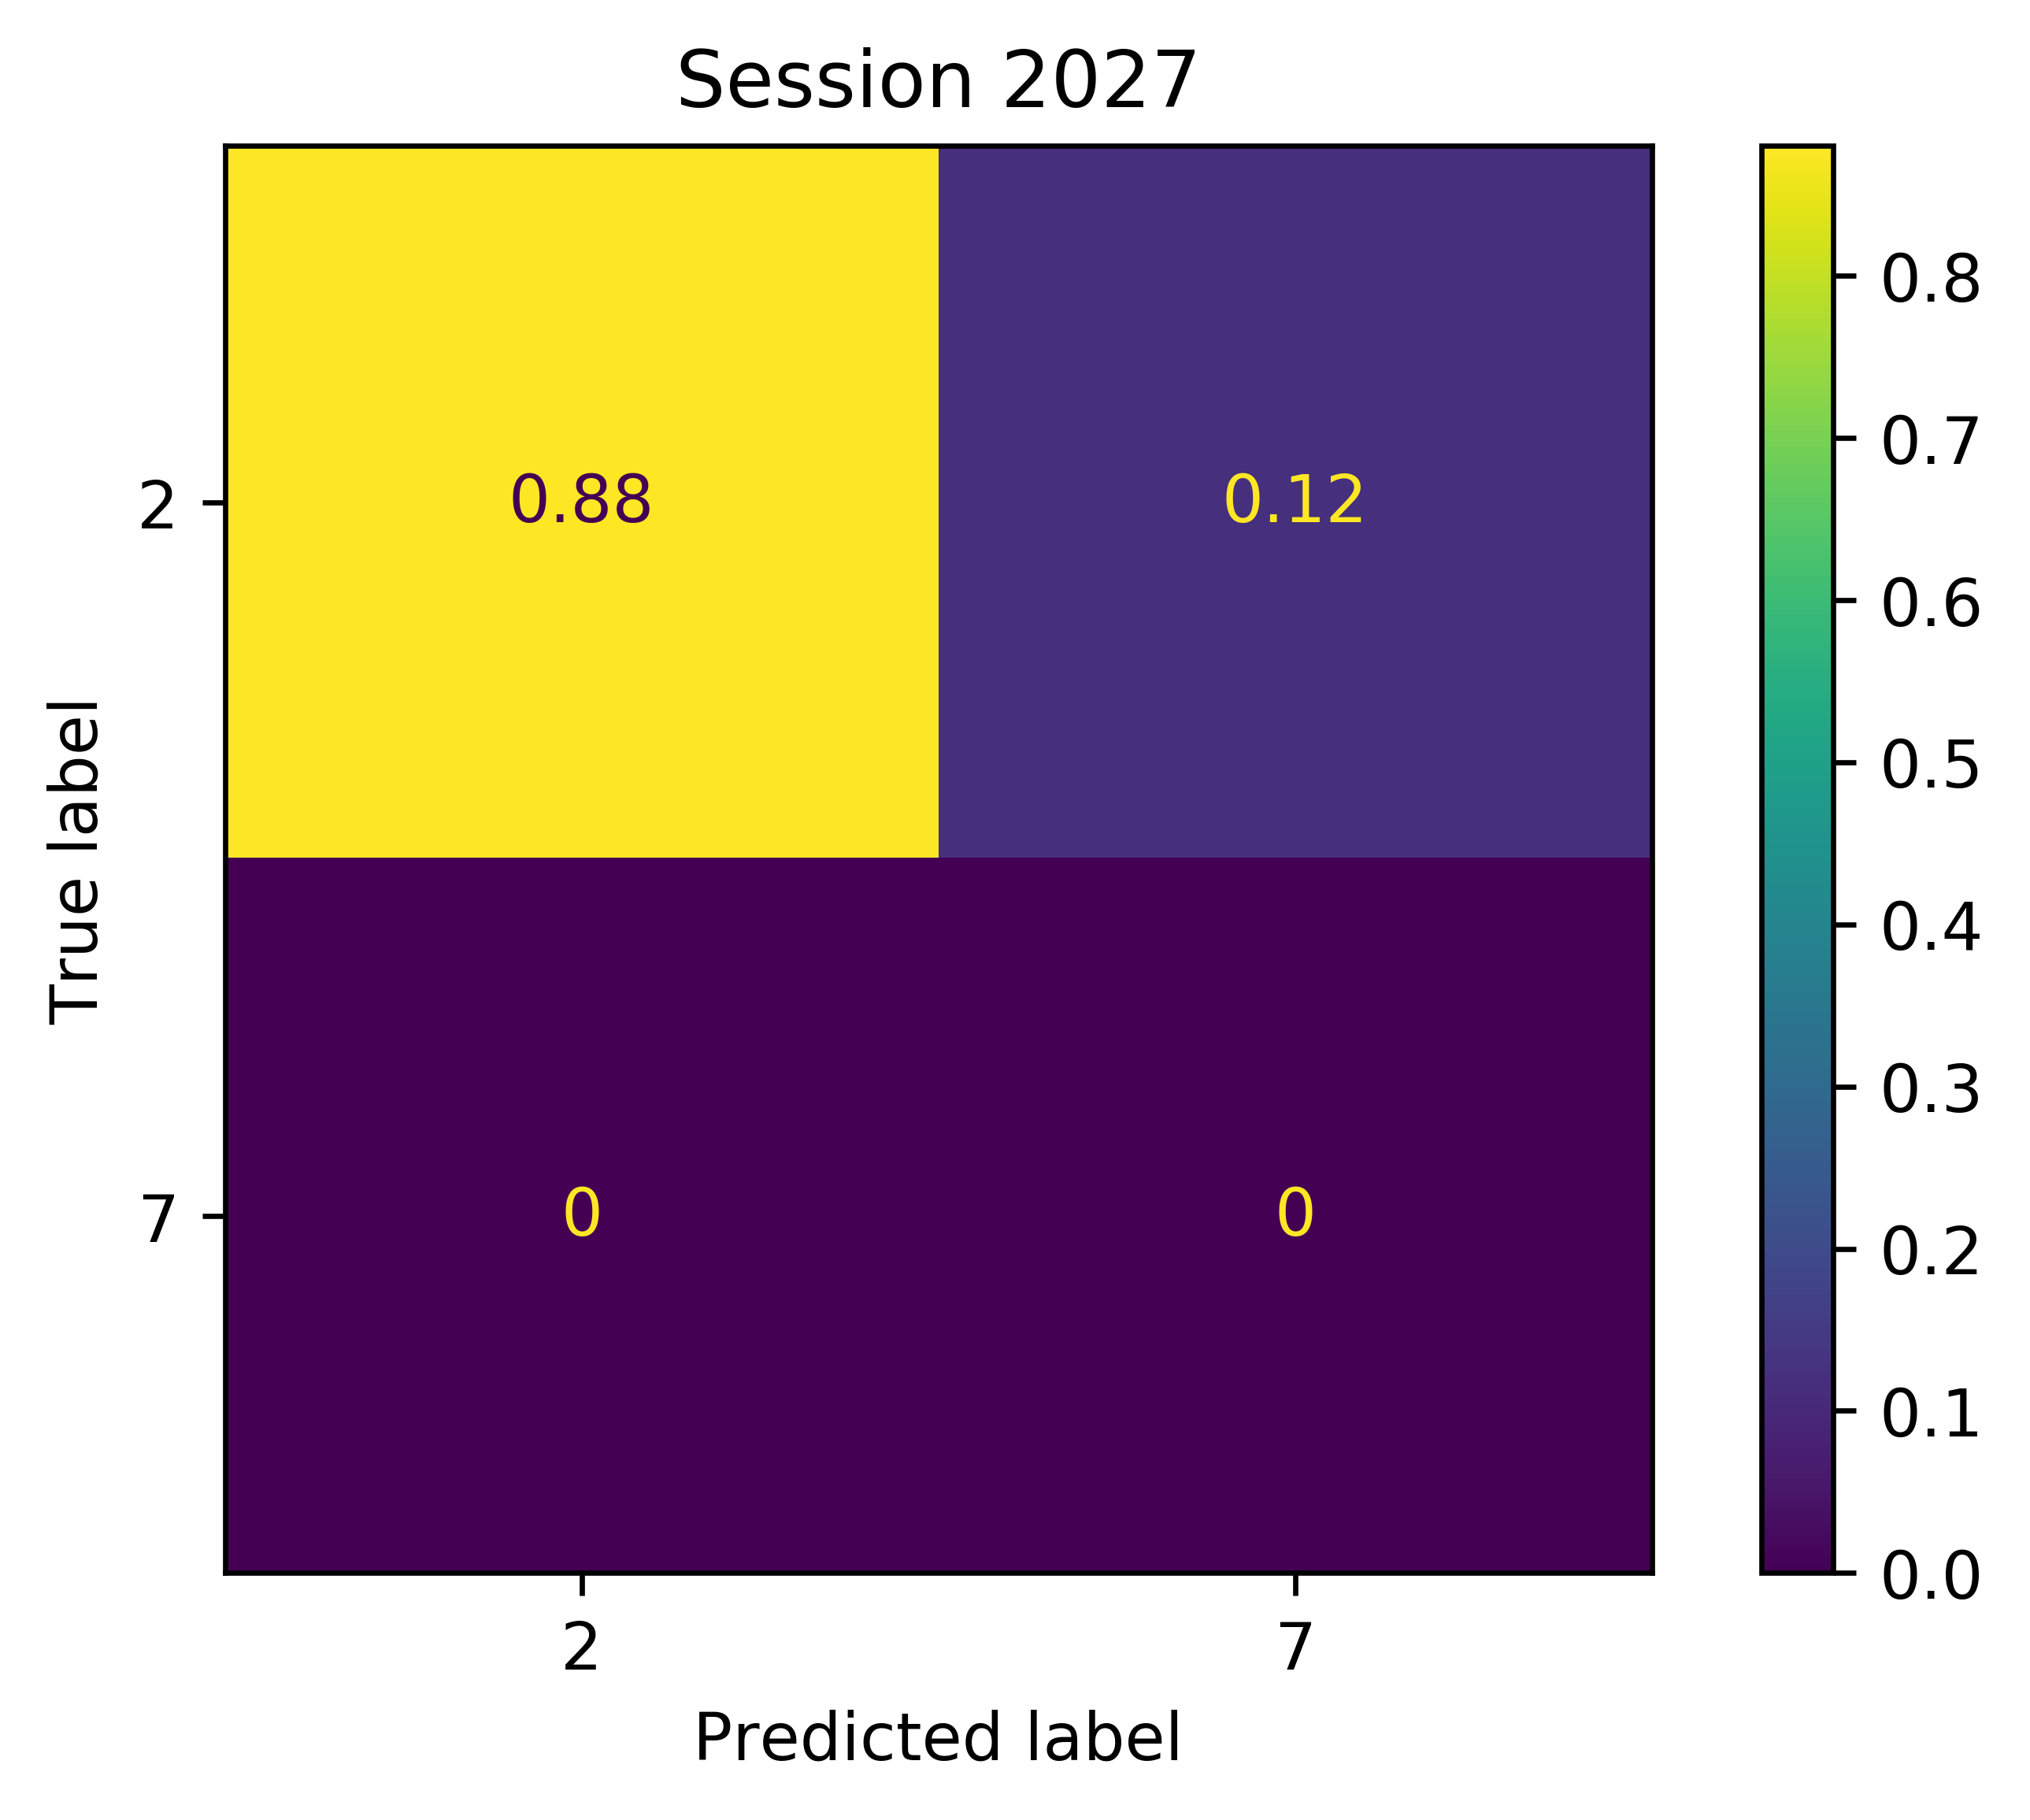
\includegraphics[width=70mm]{userCrossSessionUnf_without29/Session 2027Unf_without29.png}}
\subfigure[Session 31]{\label{fig:2031unfNo2029}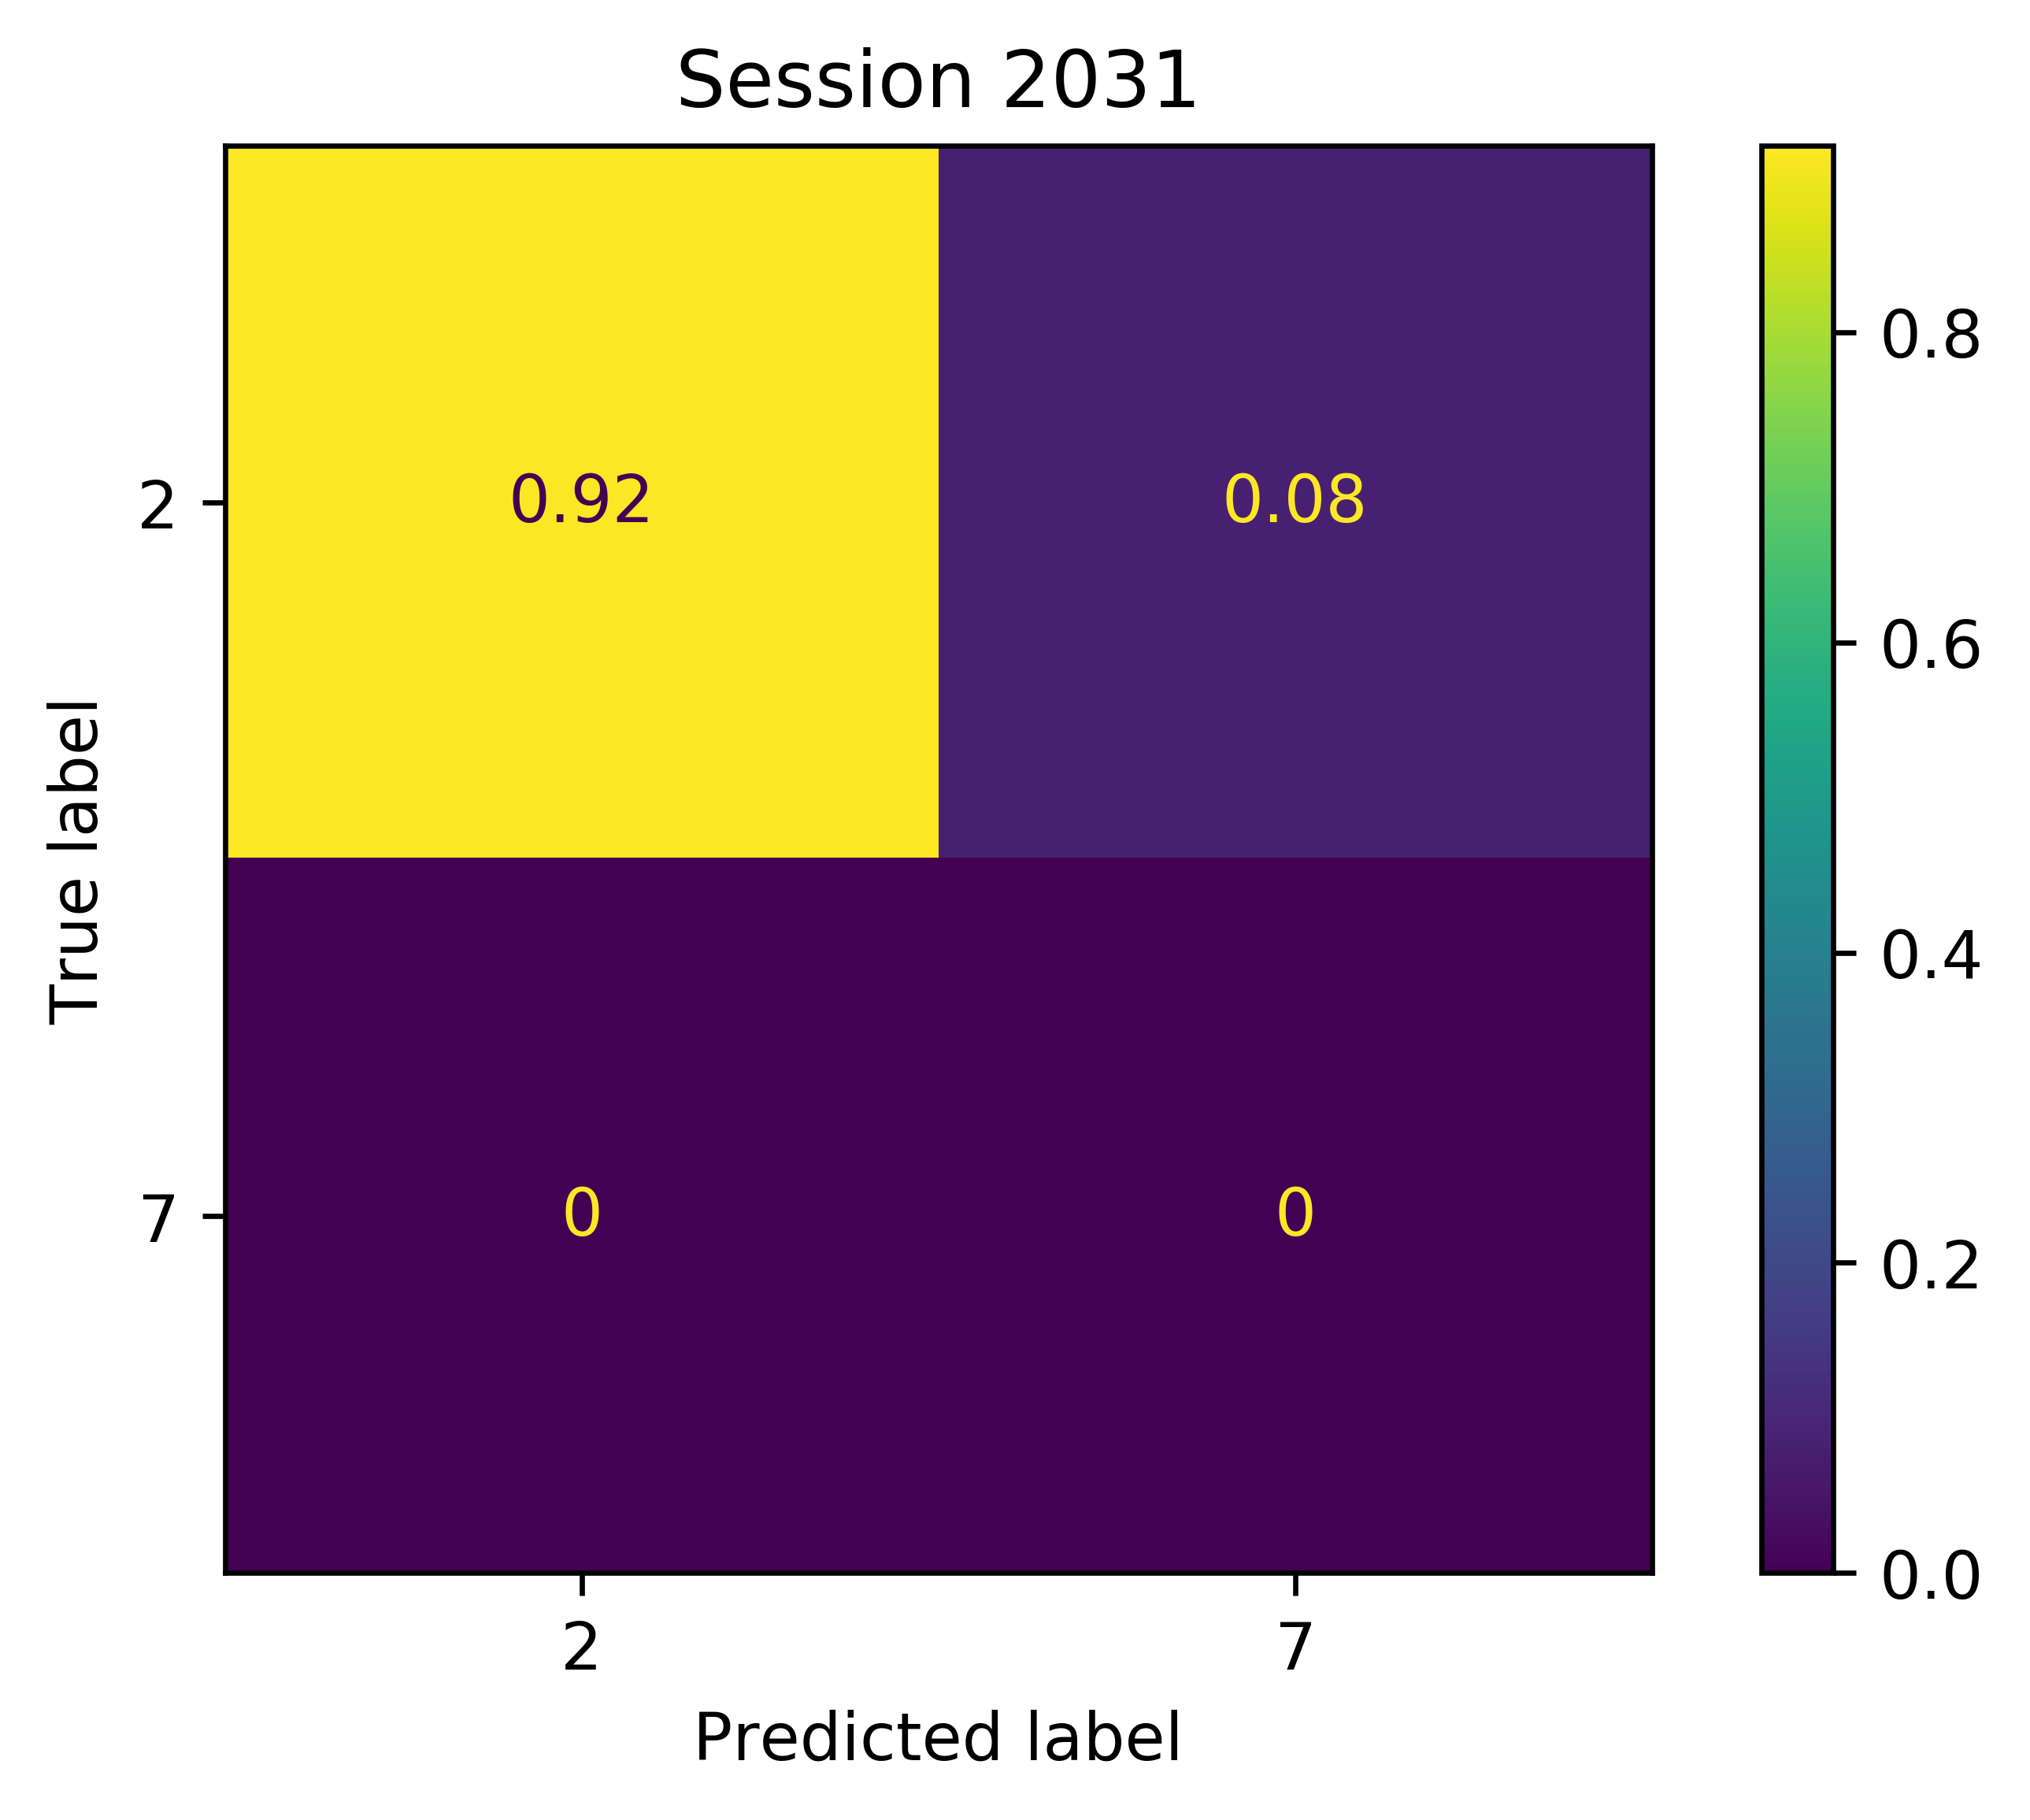
\includegraphics[width=70mm]{userCrossSessionUnf_without29/Session 2031Unf_without29.png}}
\caption{Die Erkennungsraten verschiedener Sprecher bei der Klassifizierung der Sprecheridentität in Session 27 und 31 von Sprecher 2.}
\end{figure}

\subsection{Filtered}
Hier habe ich einen Bandpassfilter(10-200Hz) auf die Daten angewendet. In der Abbildung \ref{fig:user3} kann man sehen, dass die Resultate leicht niedriger sind als bei der Variante ohne Filter. Zudem habe ich hier auf die Klassifikatoren mit einer sehr niedrigen Genauigkeit verzichtet. Man sieht in \ref{fig:Usercnf2}, das die Erkennungsraten sehr ähnlich zu den Erkennungsraten in der ungefilterten Version sind \ref{fig:Usercnf1}. Lediglich Sprecher 1 hat mit 81 Prozent eine weit niedrigere Erkennungsrate als in der ungefilterten Version. Sprecher 2 hat eine Erkennungsrate von 96 Prozent. Sprecher 4 hat eine 43 prozentige Erkennungsrate und eine 45 prozentige Verwechslungsrate mit 8. Sprecher 7 hat eine 36 prozentige Erkennungsrate und eine 36 prozentige Verwechslungsrate mit 2 und 28 prozentige Verwechslungsrate mit 8.

\begin{figure}[H]
\centering     %%% not \center
\subfigure[Sprecher 1,2,4,7 und 8]{\label{fig:user3}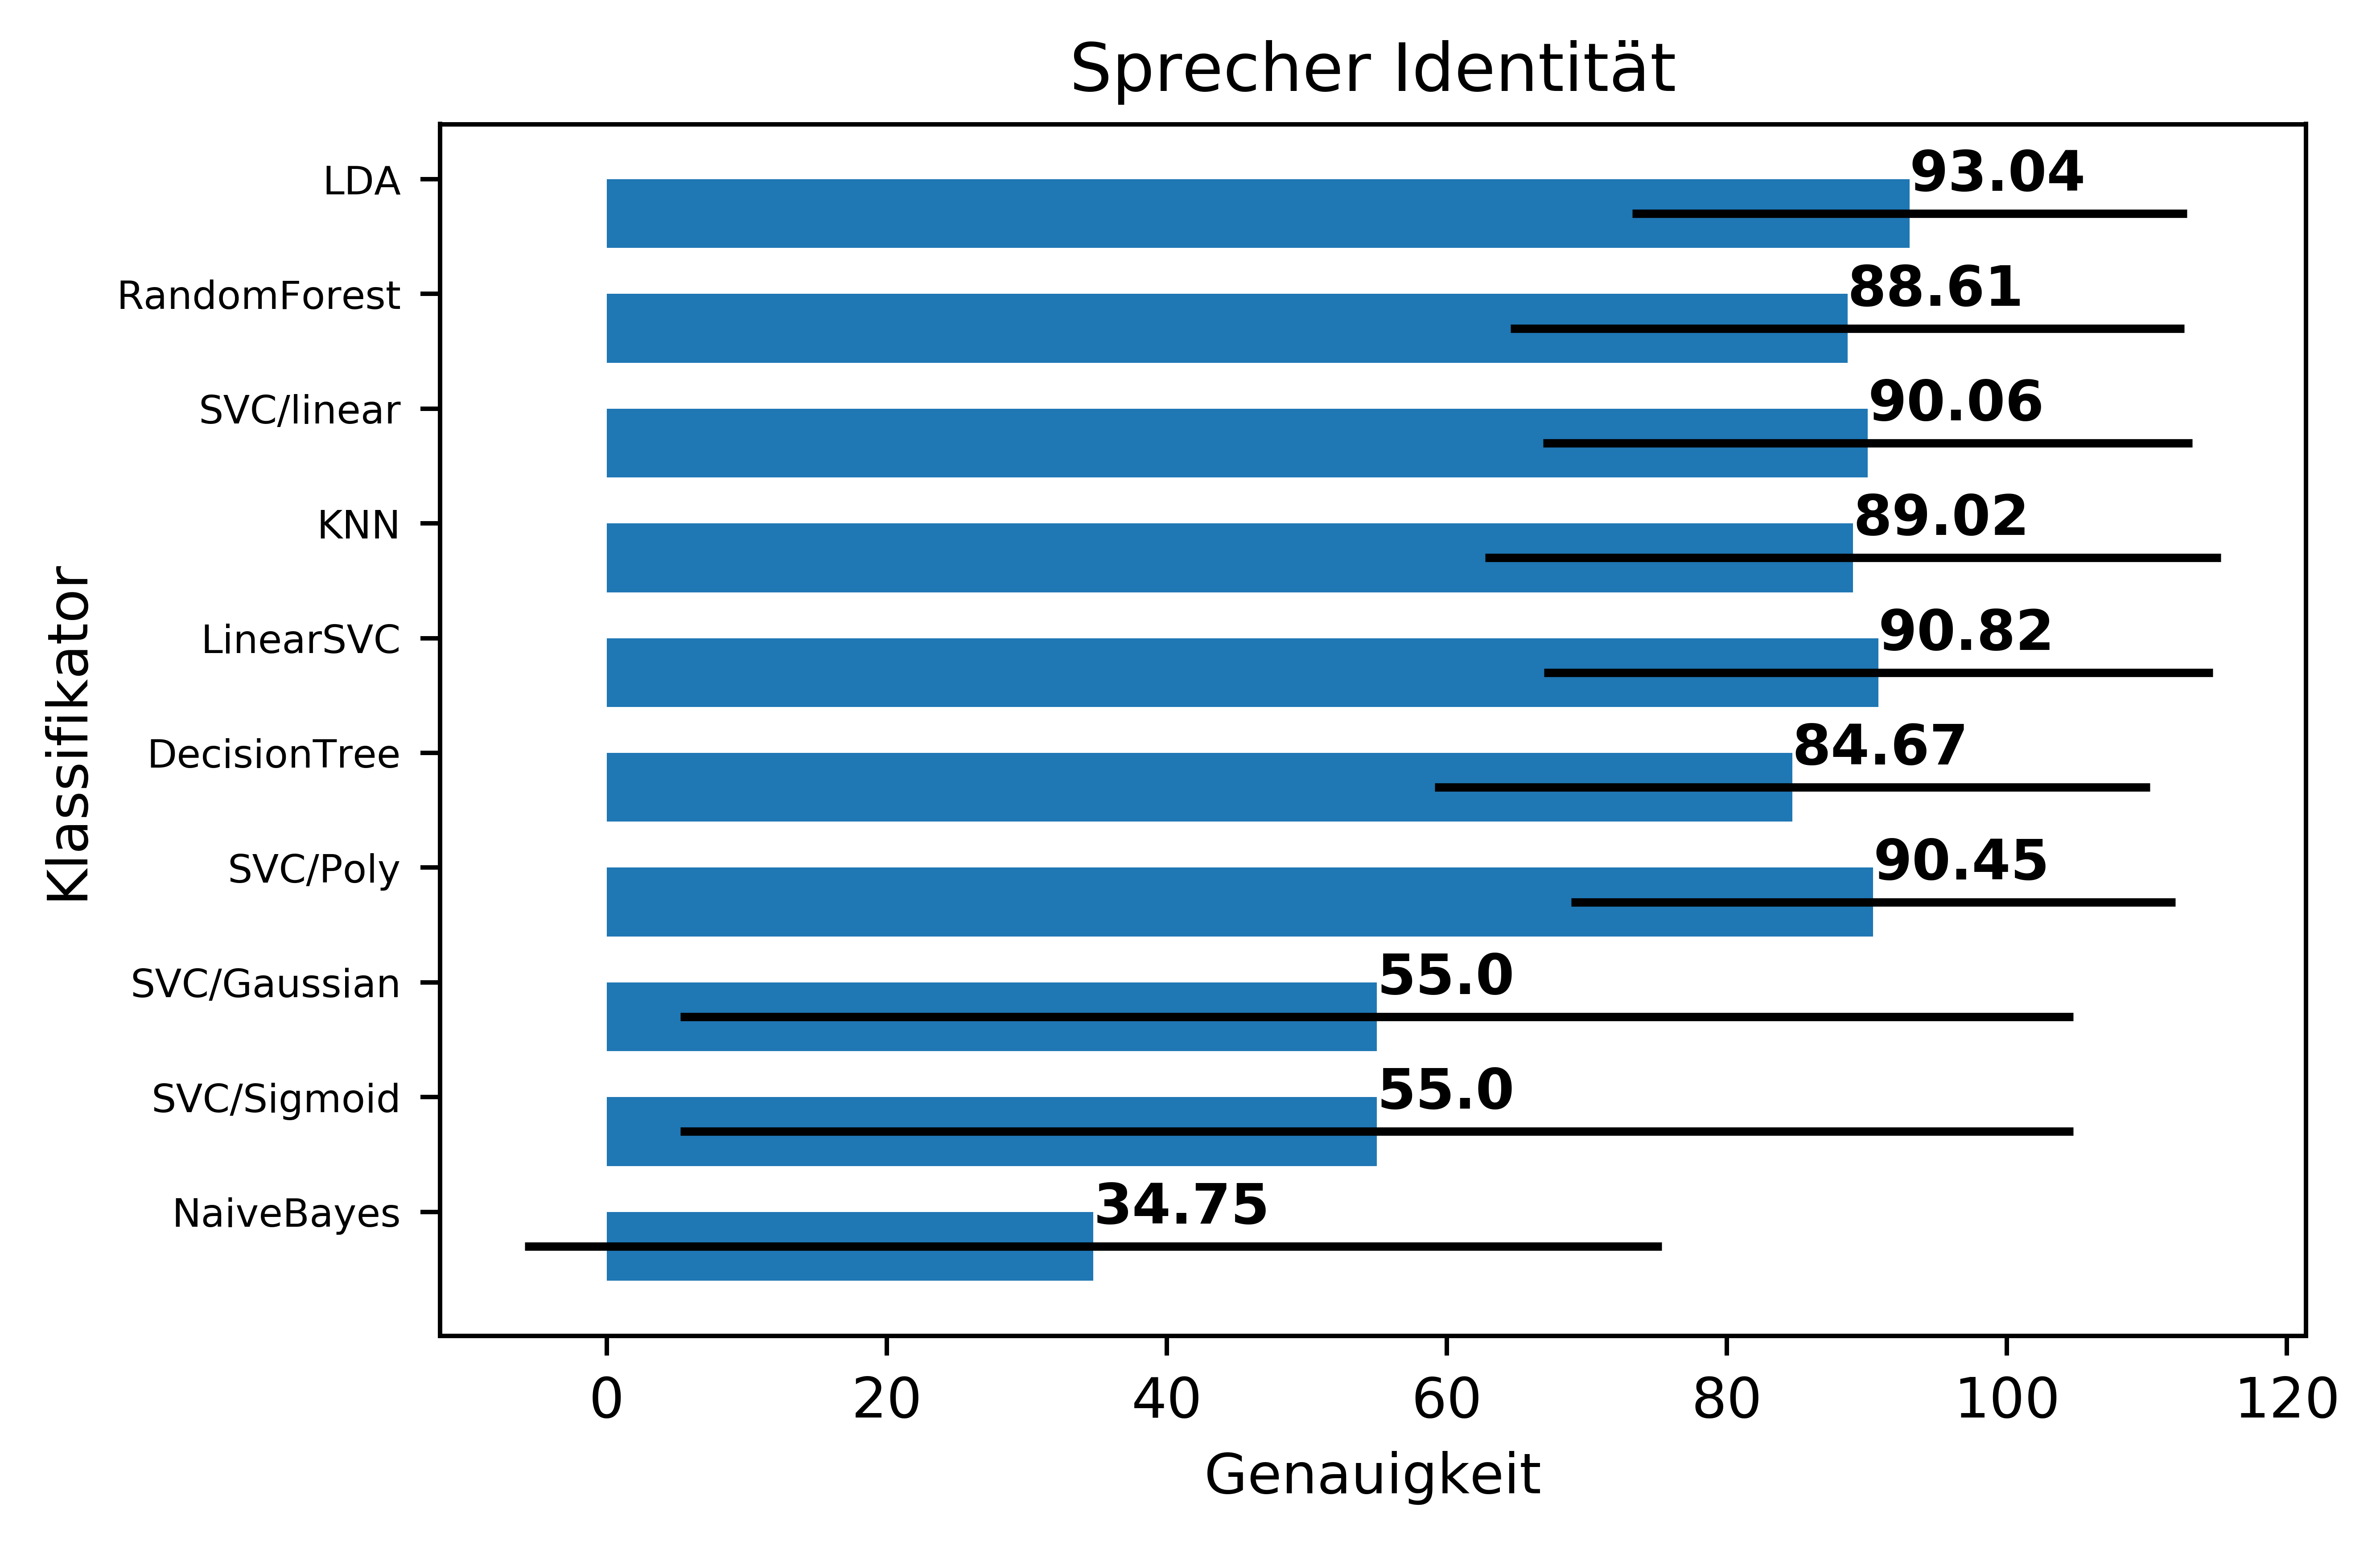
\includegraphics[width=70mm]{UserResults10too200hz.png}}
\subfigure[Sprecher 2 und 8]{\label{fig:user4}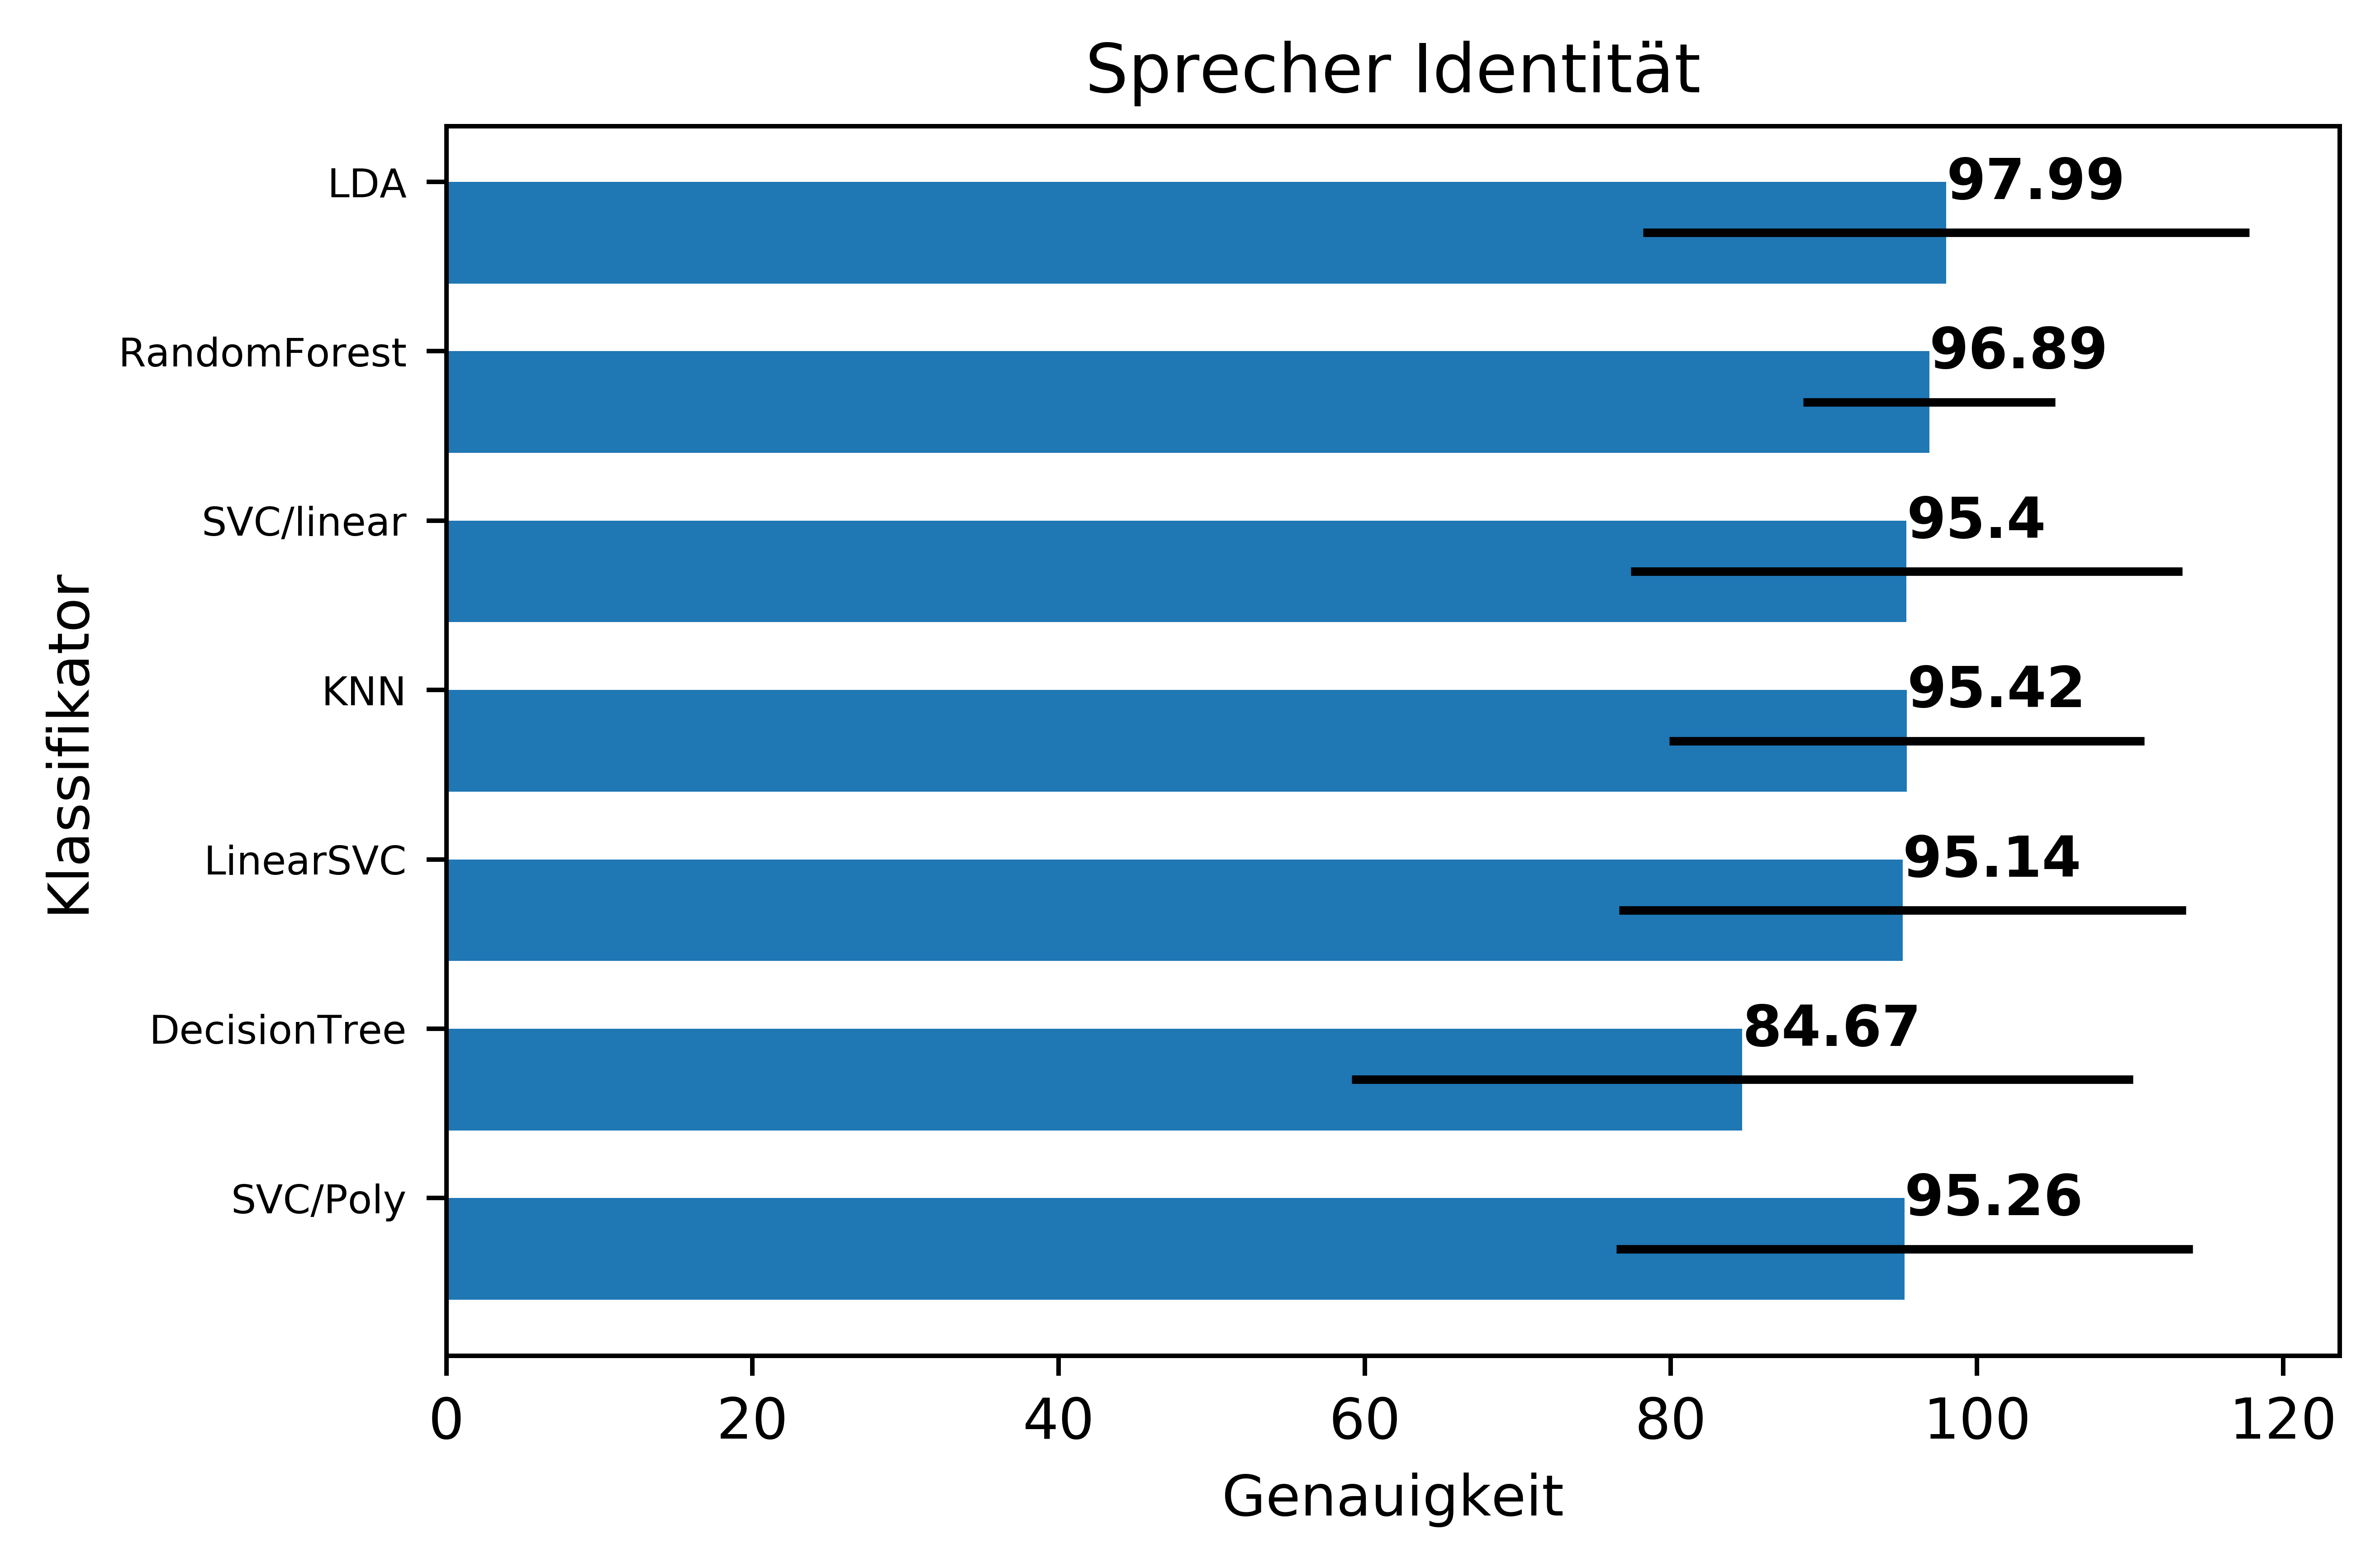
\includegraphics[width=70mm]{UserResults10too200hz2User.png}}
\caption{Die durchschnittliche Genauigkeit, sowie die Standardabweichung der verschiedener Klassifikatoren bei der Erkennung der Sprecheridentität.}
 \label{fig:vergleich}
\end{figure}

\begin{figure}[H]
  \centering
  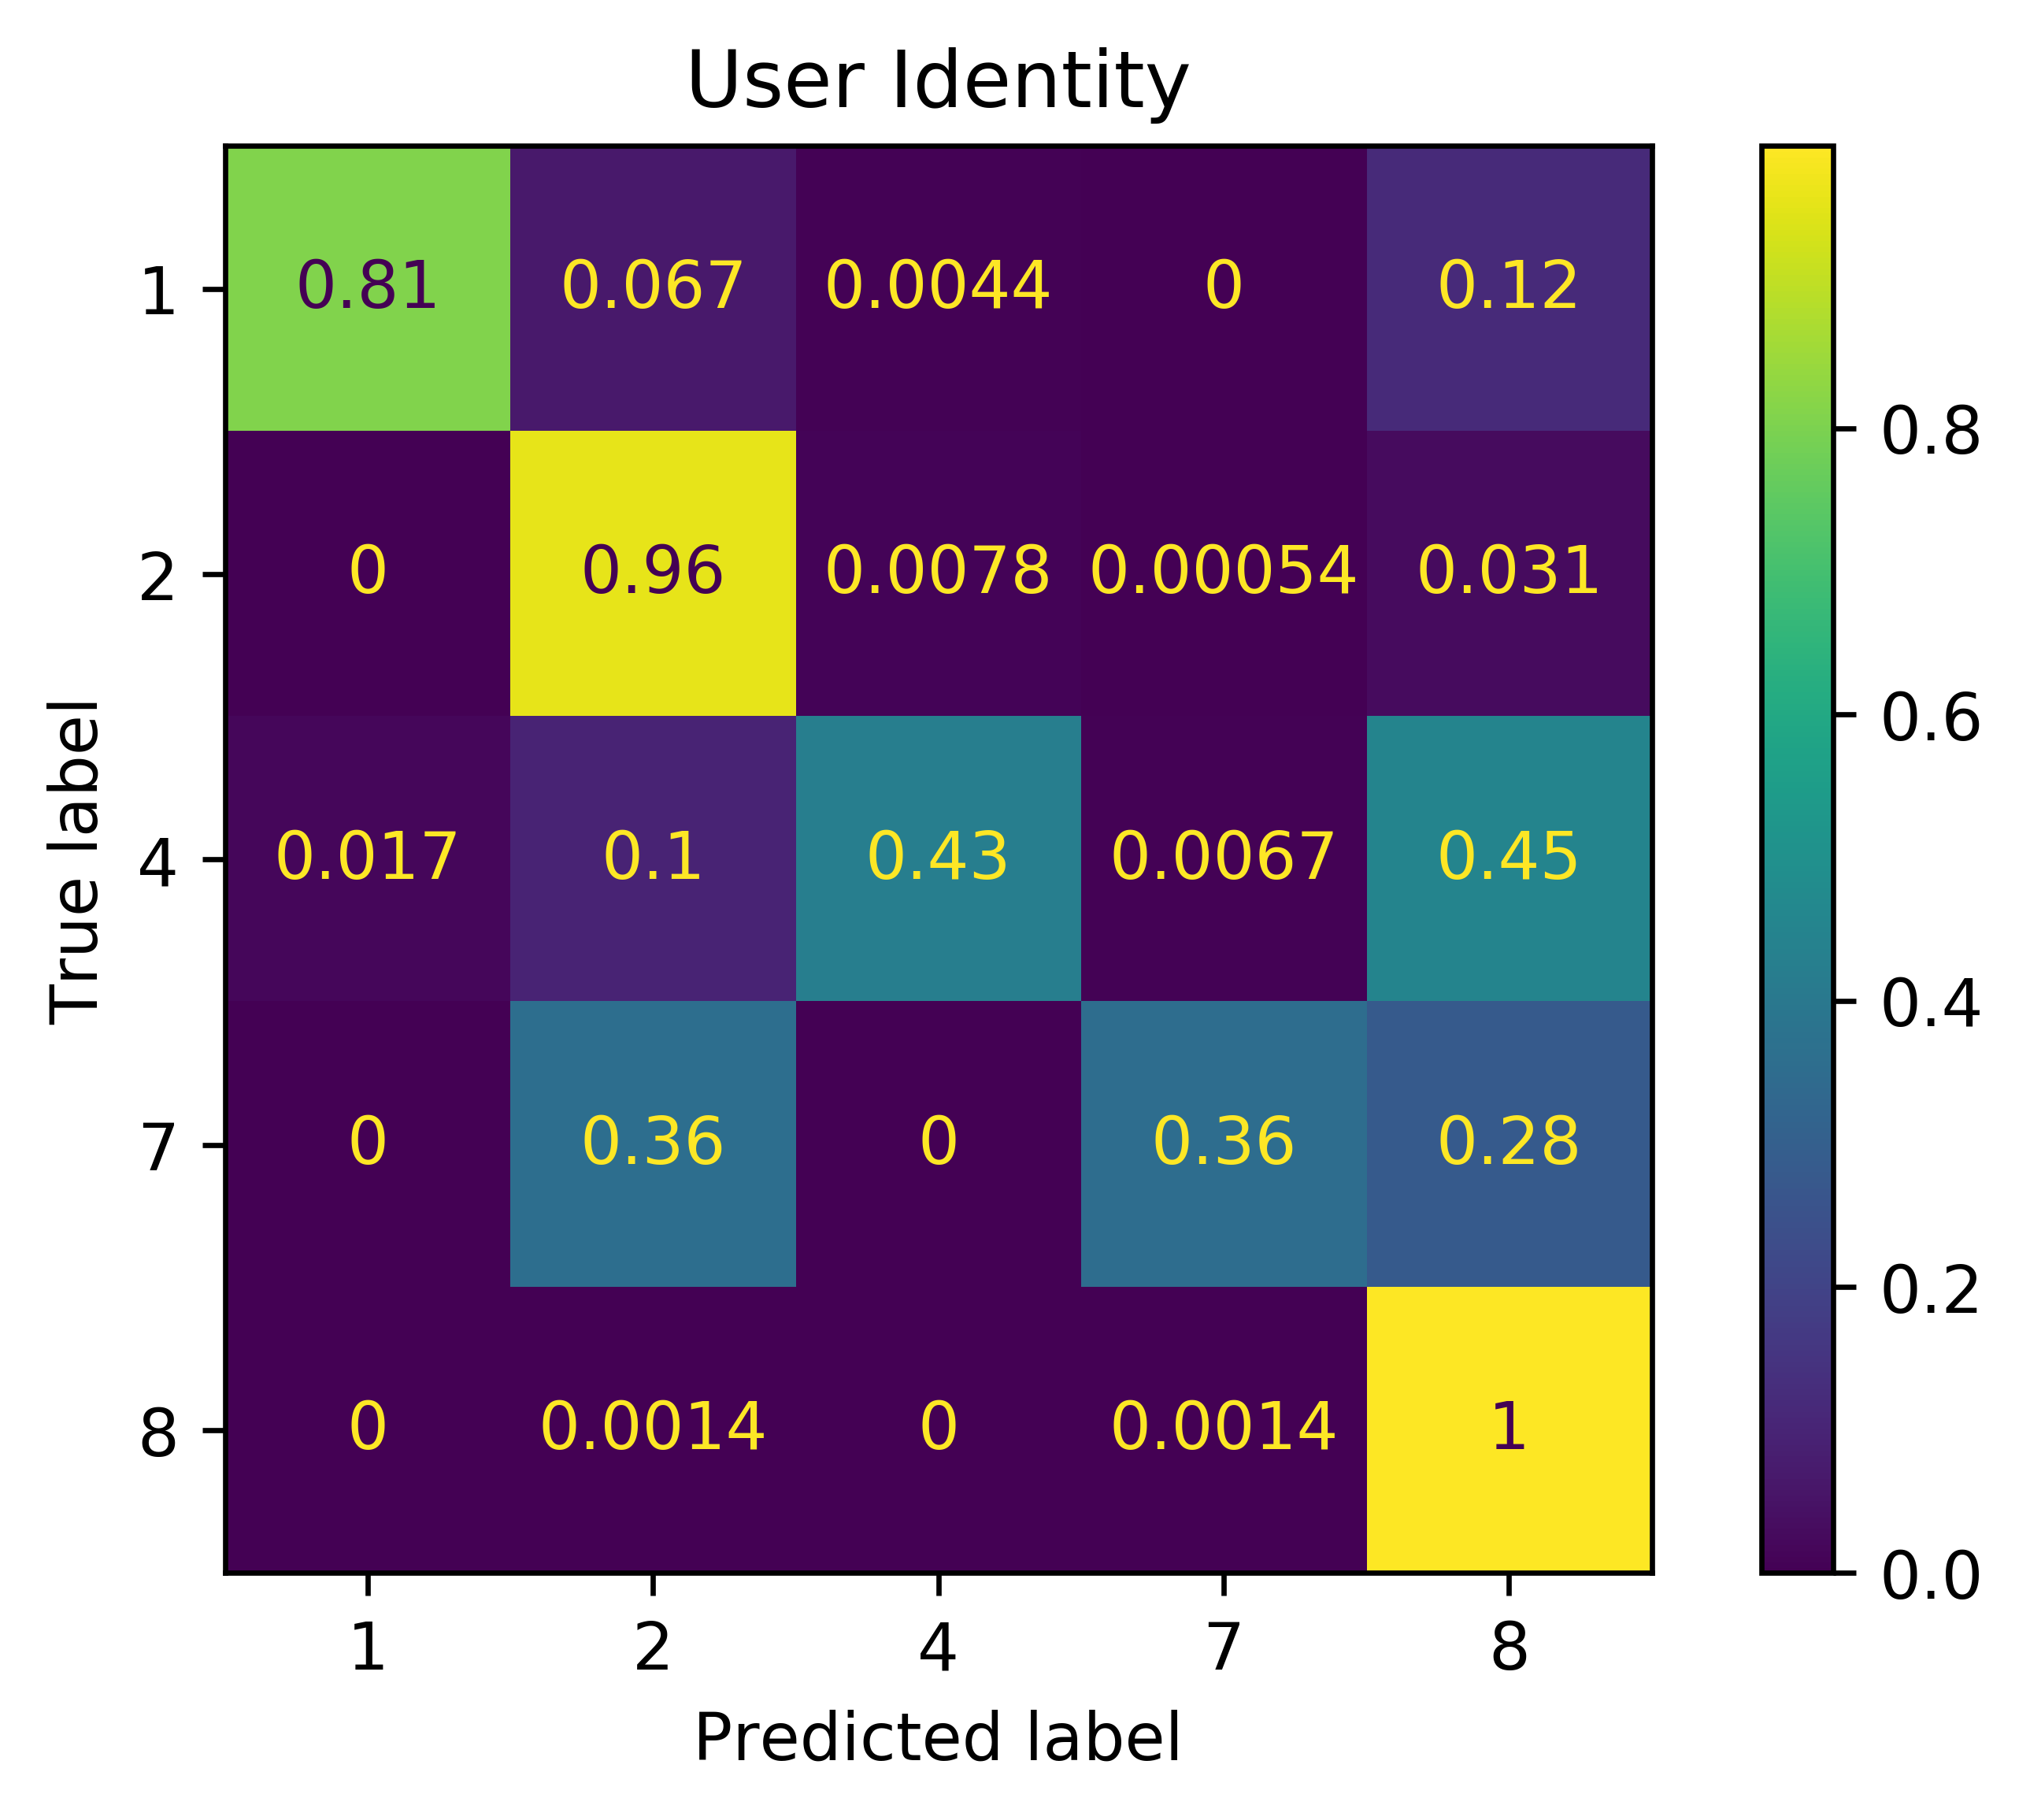
\includegraphics[width=90mm ,scale=0.6]{AllUserConfMat.png}
  \caption{Die Confusion-Matrix der Erkennung Sprecheridentität mit gefilterten Daten.}
  \label{fig:Usercnf2}
\end{figure}

Bei diesen Tests viel auf, dass die Genauigkeit für die Sprecher mit weniger Daten vergleichbar viel niedriger ist als die Genauigkeit für die anderen Sprecher. Deshalb wurde ein zweiter Versuch gemacht, indem nur die Daten von Sprecher 2 und 8 verwendet wurden. Dabei waren die Resultate deutlich besser als in dem vorherigen versuch (siehe \ref{fig:vergleich}). Die Resultate hier sind leicht niedrigerer als bei der ungefilterten Variante.


\subsubsection{Sessions}
In der Tabelle \ref{tab:FilteredSessions} sieht man die Genauigkeit für jede Session. Die Sessions mit 100 Prozent Genauigkeit wurden entfernt.
Die meisten der Sessions für Sprecher 8 und 2 hatten hier eine Genauigkeit von 100 Prozent. Es gibt jedoch einzelne Sessions die deutlich geringere Genauigkeiten aufweisen. In Sprecher 2 sieht man zum Beispiel in den Sessions 29 und 26 eine viel geringere Genauigkeit als bei allen anderen Sessions. Ich gehe, wie bei der ungefilterten Version, davon aus das in diesen Sessions Fehler bei der Aufnahme passiert sind. Bei Sprecher 8 mit einer vergleichbaren Anzahl an Sessions sind solche Ausnahmen nämlich in Sprecher 8 auch nicht zu sehen.

\begin{table}[H]
 \centering
 \caption{Genauigkeiten aller Sessions bei der Sprecher Erkennung mit gefilterten Daten.}
\begin{tabular}{|c|c|}
\hline 
Session & Resultat in Prozent \\ 
\hline 
1001 & 66 \\ 
\hline 
1002 & 81,33 \\ 
\hline 
1003 & 95,33 \\ 
\hline 
2002 & 98 \\ 
\hline 
2015 & 98 \\ 
\hline 
2026 & 68 \\  
\hline 
2029 & 26,67 \\ 
\hline 
4001 & 85.33 \\ 
\hline 
4002 & 0 \\ 
\hline 
7001 & 36 \\ 
\hline 
7002 & 34.67 \\ 
\hline 
8006 & 96 \\ 
\hline 
\label{tab:FilteredSessions} 
\end{tabular} 
\end{table}

In \ref{fig:cnf5} sieht man das in über 73 Prozent der Fälle Sprecher 2 mit Sprecher 8 verwechselt wird. In Session 26 sieht man mit 32 Prozent ebenfalls eine hohe Verwechslungs-rate mit Sprecher 8 und zudem noch eine 17 Prozent Verwechslungs-rate mit Sprecher 7. Die restlichen Sessions von Sprecher 2 haben entweder eine Genauigkeit von 100 Prozent oder haben nur sehr wenige Verwechslungen mit dem anderen Sprechern.

\begin{figure}[H]
  \centering
  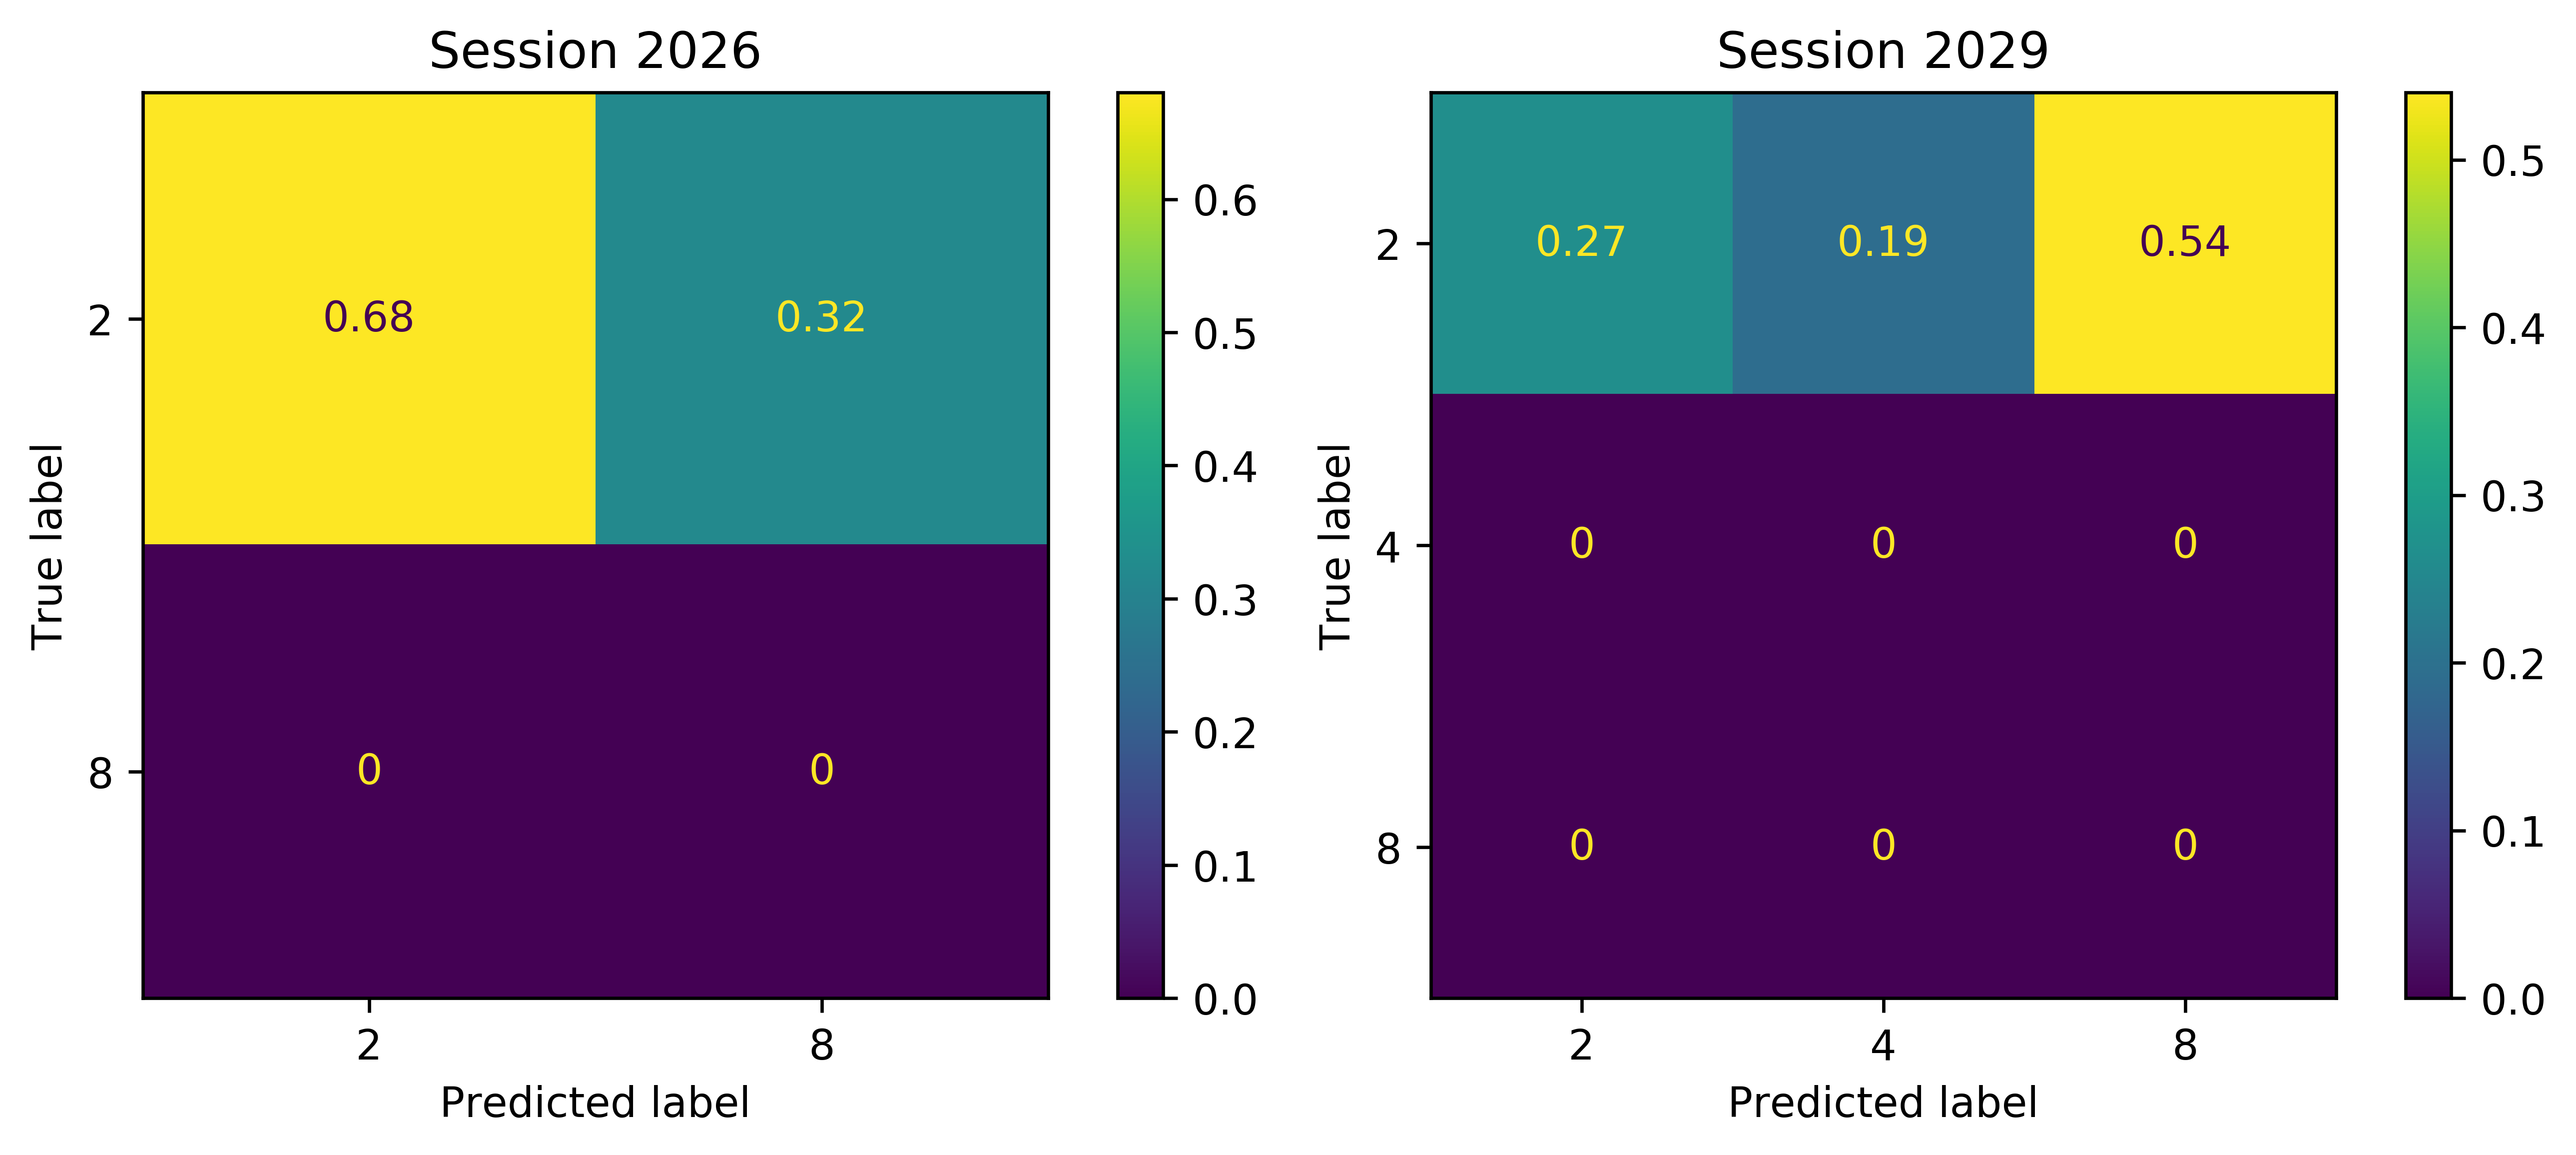
\includegraphics[width=100mm ,scale=0.6]{UserConfMatUser2.png}
  \caption{Confusion-Matrix der Session 29 und 26 von Sprecher 2}
  \label{fig:cnf5}
\end{figure}

Für Sprecher 4 in Session 2 und für Sprecher 7 in beiden Sessions sieht man eine weit niedrigere Genauigkeit als in den Sessions der anderen Sprecher, dasselbe lässt sich für Sprecher 1 weniger stark betrachten. Hier hat die erste Session eine Genauigkeit von 66 Prozent und die zwei anderen Sessions jeweils eine Genauigkeit von 81.33 und 95.33 Prozent. Die Genauigkeit ist hier niedriger als bei der ungefilterten Version. Bei Sprecher 4 ist die Genauigkeit bei der zweiten Session 0 und bei der ersten Session sehr hoch. In \ref{fig:cnf6} sieht man die Zusammensetzung dieser Genauigkeit. Anders als bei der ungefilterten Variante haben wir hier nämlich in der zweiten Session kaum Sprecher 1 vorhersagen, dafür sind jetzt 90 Prozent der vorhersagen Sprecher 8.

\begin{figure}[H]
  \centering
  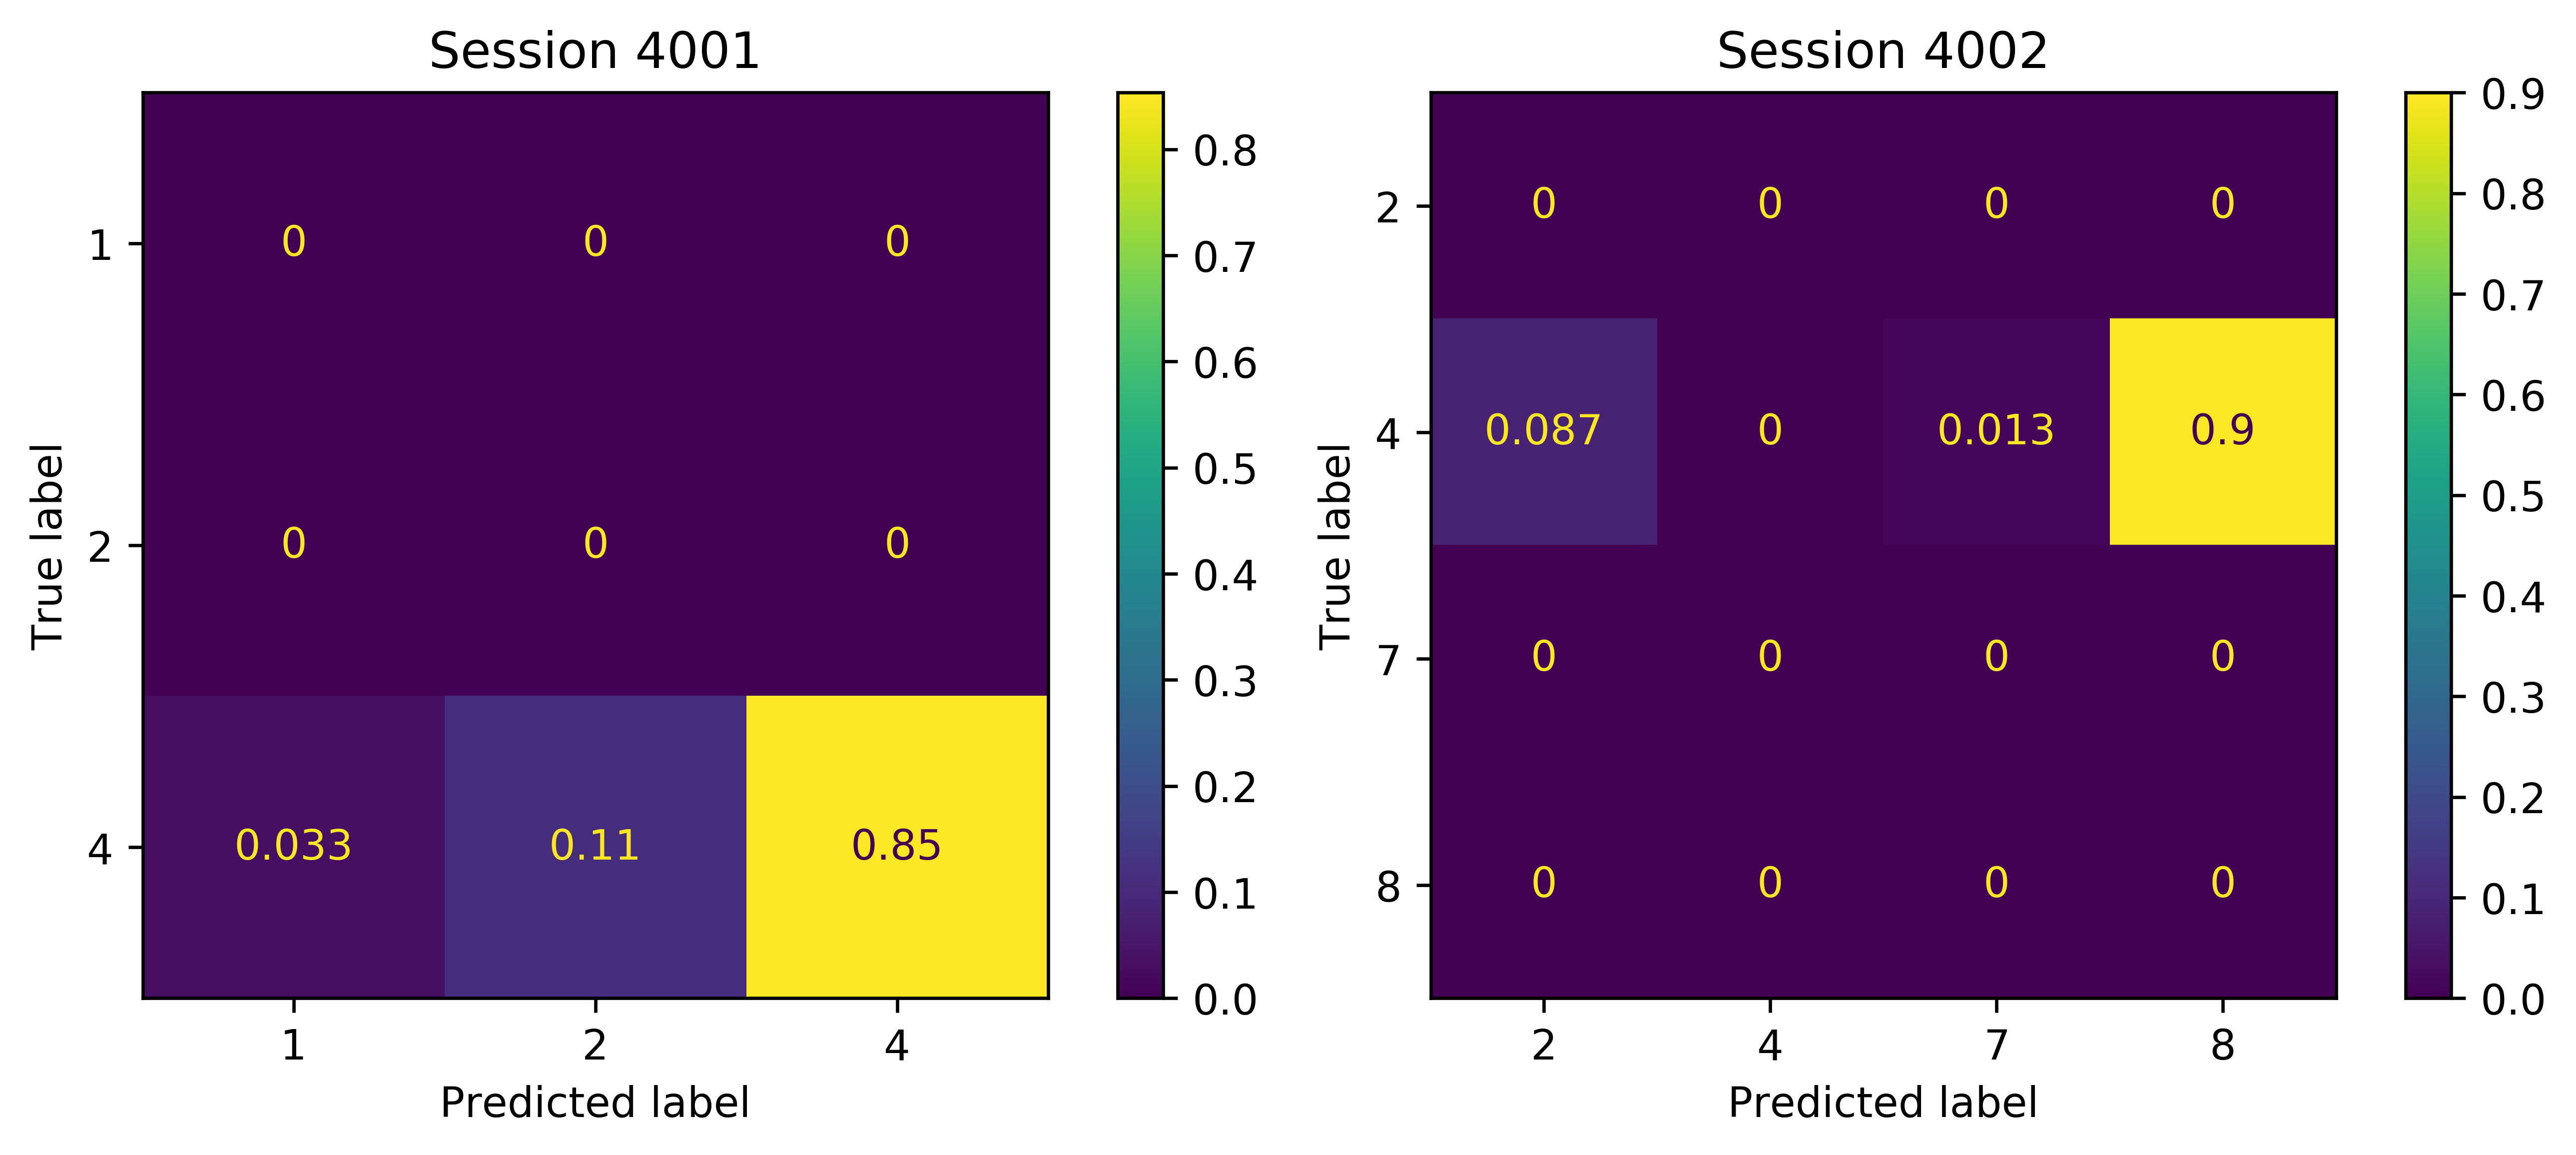
\includegraphics[width=100mm ,scale=0.4]{UserConfMatUser4.png}
  \caption{Die Confusion-Matrix der beiden Session für Sprecher 4}
  \label{fig:cnf6}
\end{figure}

Meine Vermutung ist das es nicht nur auf die Anzahl der Sessions, sondern auch auf die Qualität der Sessions ankommt die Gründe hierfür sind dieselben wie für die gefilterte Variante.
Bei diesen Tests ist aufgefallen, dass die Genauigkeit für die Sprecher mit weniger Daten vergleichbar viel niedriger ist als die Genauigkeit für die anderen Sprecher. 
\paragraph{}
Deshalb wurde ein zweiter Versuch durchgeführt in dem nur die Daten der Sprecher 2 und 8 genutzt wurden. Dabei waren die Resultate deutlich besser als in dem vorherigen Versuch (siehe \ref{fig:user2}) haben sich aber nicht zu sehr verändert, denn die Fehler in der Genauigkeit passieren größtenteils, wenn Sprecher 2 und Sprecher 8 verwechselt werden. Wie man in der Confusion Matrix von Session 29 sowie Session 26 von Sprecher 2 sehen kann. Die kleinen Unterschiede im 95–99 Prozent Bereich belaufen sich meisten auch auf das Vertauschen von Sprecher 2 und Sprecher 8.

\paragraph{Session 29 entfernt} 
Bei den Ergebnissen dieses Versuchs ist eine Steigerung der Genauigkeit, in Session 26 von Sprecher 2 von 68 auf 87 Prozent, zu beobachten(\ref{tab:FilteredSessionsNo29}). In \ref{fig:cnf7} sieht man, dass das Steigern der Genauigkeit daher kommt das Sprecher 8 seltener geraten wird. Nähere Analysen wurden hier weggelassen, weil sie sehr ähnlich zu der ungefilterten Variante sind.

\begin{table}[H]
 \centering
 \caption{Genauigkeiten aller Sessions bei der Erkennung der Sprecheridentität. Es werden die Resultate der gefilterten Daten mit den Resultaten der ungefilterten verglichen.}
\begin{tabular}{|c|c|c|c|}
\hline 
Session & Resultat(filter) & Resultat ohne & Veränderung \\ 
\hline 
1001 & 66 & 61.33 & -4.67 \\ 
\hline 
1002 & 81,33 & 82 & -0.67 \\ 
\hline 
1003 & 95,33 & 91.33 & -4 \\ 
\hline 
2001 & 99.33 & 98 & -1.33 \\  
\hline 
2002 & 98 & 100 & +2\\ 
\hline 
2026 & 68 & 87 & +19 \\ 
\hline 
2027 & 93 & 100 & +7 \\ 
\hline 
2031 & 96 & 100 & +4\\ 
\hline 
4001 & 85.33 & 97.33 & +12.67 \\ 
\hline 
4002 & 0 & 0 & 0 \\ 
\hline 
7001 & 36 & 36 & 0 \\ 
\hline 
7002 & 34.67 & 34,67 & 0\\ 
\hline 
8006 & 96 & 96 & 0 \\
\hline
\label{tab:FilteredSessionsNo29} 
\end{tabular}
\end{table}

\begin{figure}[H]
  \centering
  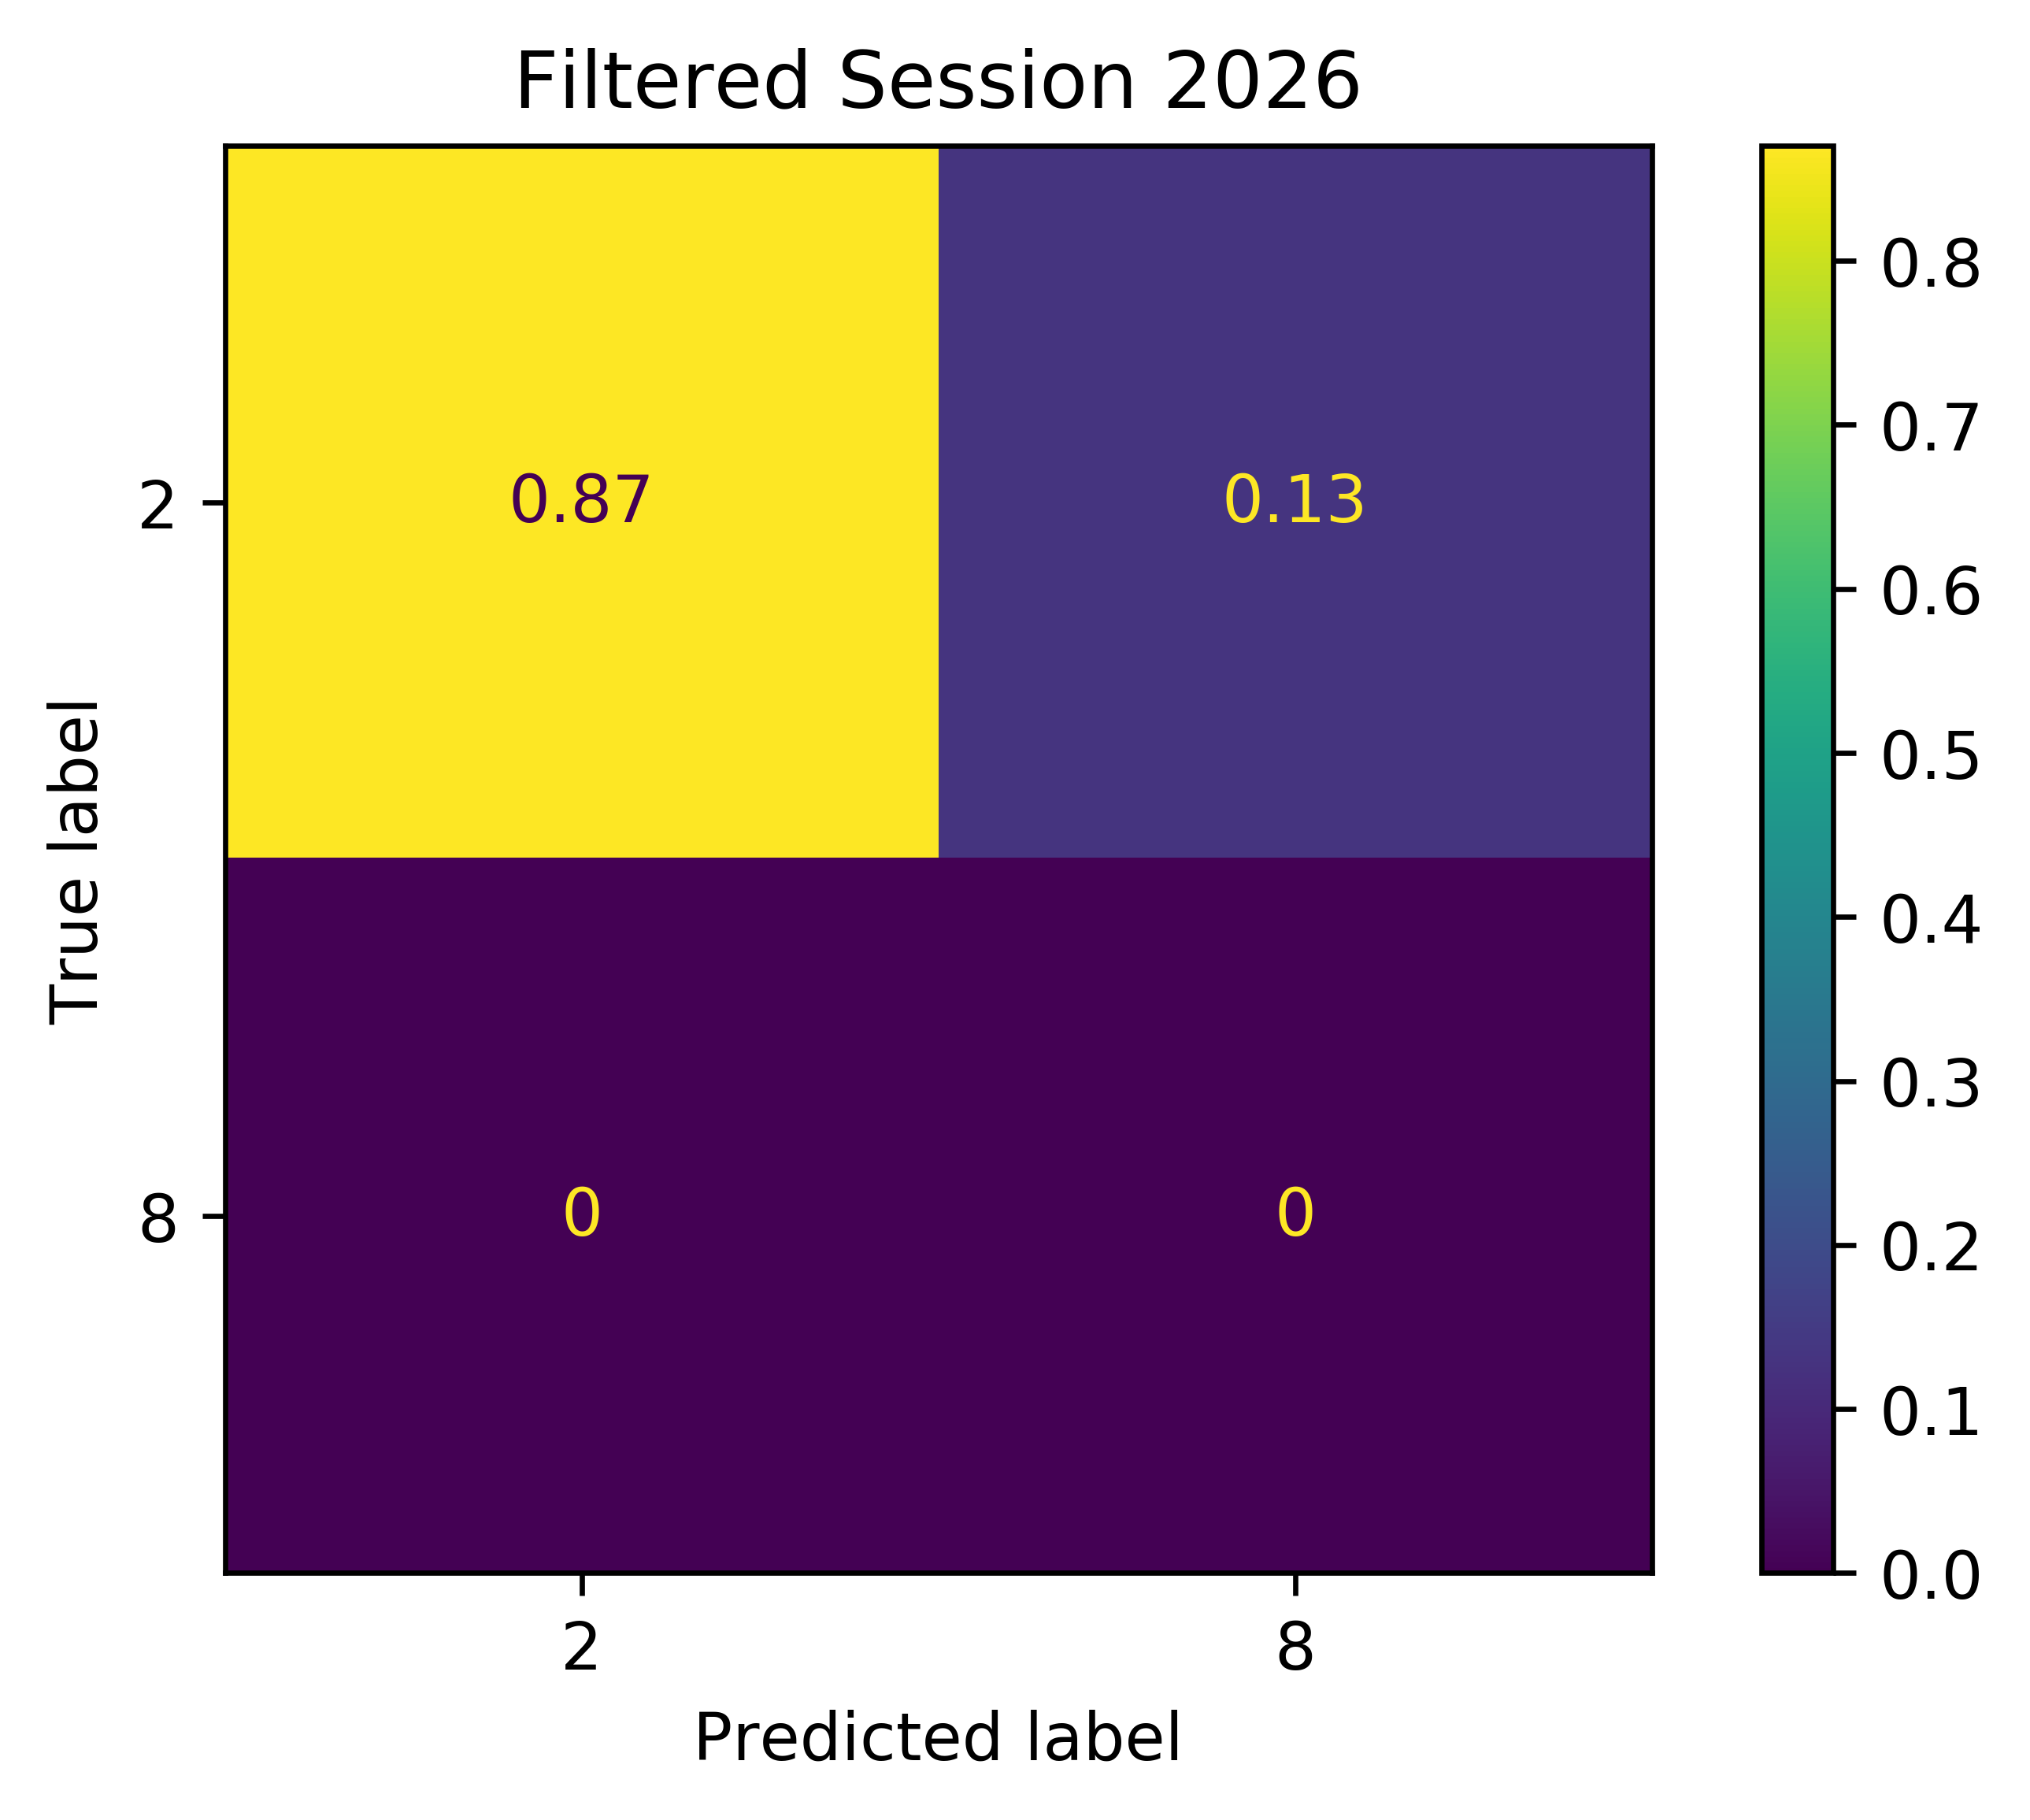
\includegraphics[width=80mm ,scale=0.4]{userCrossSession_without29/Session 2026_without29.png}
  \caption{Die Confusion-Matrix der 26. Session von Sprecher 2}
  \label{fig:cnf7}
\end{figure}


\section{Sprachmodus}
\subsection{Cross-Session}
In(\ref{fig:mode1} und \ref{fig:mode2}) wurden die Daten für die Experimente so aufgeteilt das alle Sessions, welche alle drei Sprachmodi enthalten genutzt wurden. Es wurde mit allen Sessions außer einer Trainiert und auf der ausgelassenen Session wurde getestet. Die Genauigkeiten in den unteren Graphen ist dabei der durchschnittliche Wert zwischen den Resultaten von allen Sessions.

\subsubsection{Ungefiltert}
 Hier(\ref{fig:mode1}) ist eine sehr gleichmäßig verteile Genauigkeit über alle Klassifikatoren zu betrachten wobei der Lda, der Randomforest sowie der LinerSVC die höchsten Werte vorweisen. Der LDA-Klassifikator mit 59.6 Prozent bietet die höchste Genauigkeit. Der KNN-Klassifikator und der DecisionTree Klassifikator haben die niedrigsten Genauigkeiten wobei DecisionTree mit 46.88 Prozent die niedrigste Genauigkeit hat.

\begin{figure}[H]
  \centering
  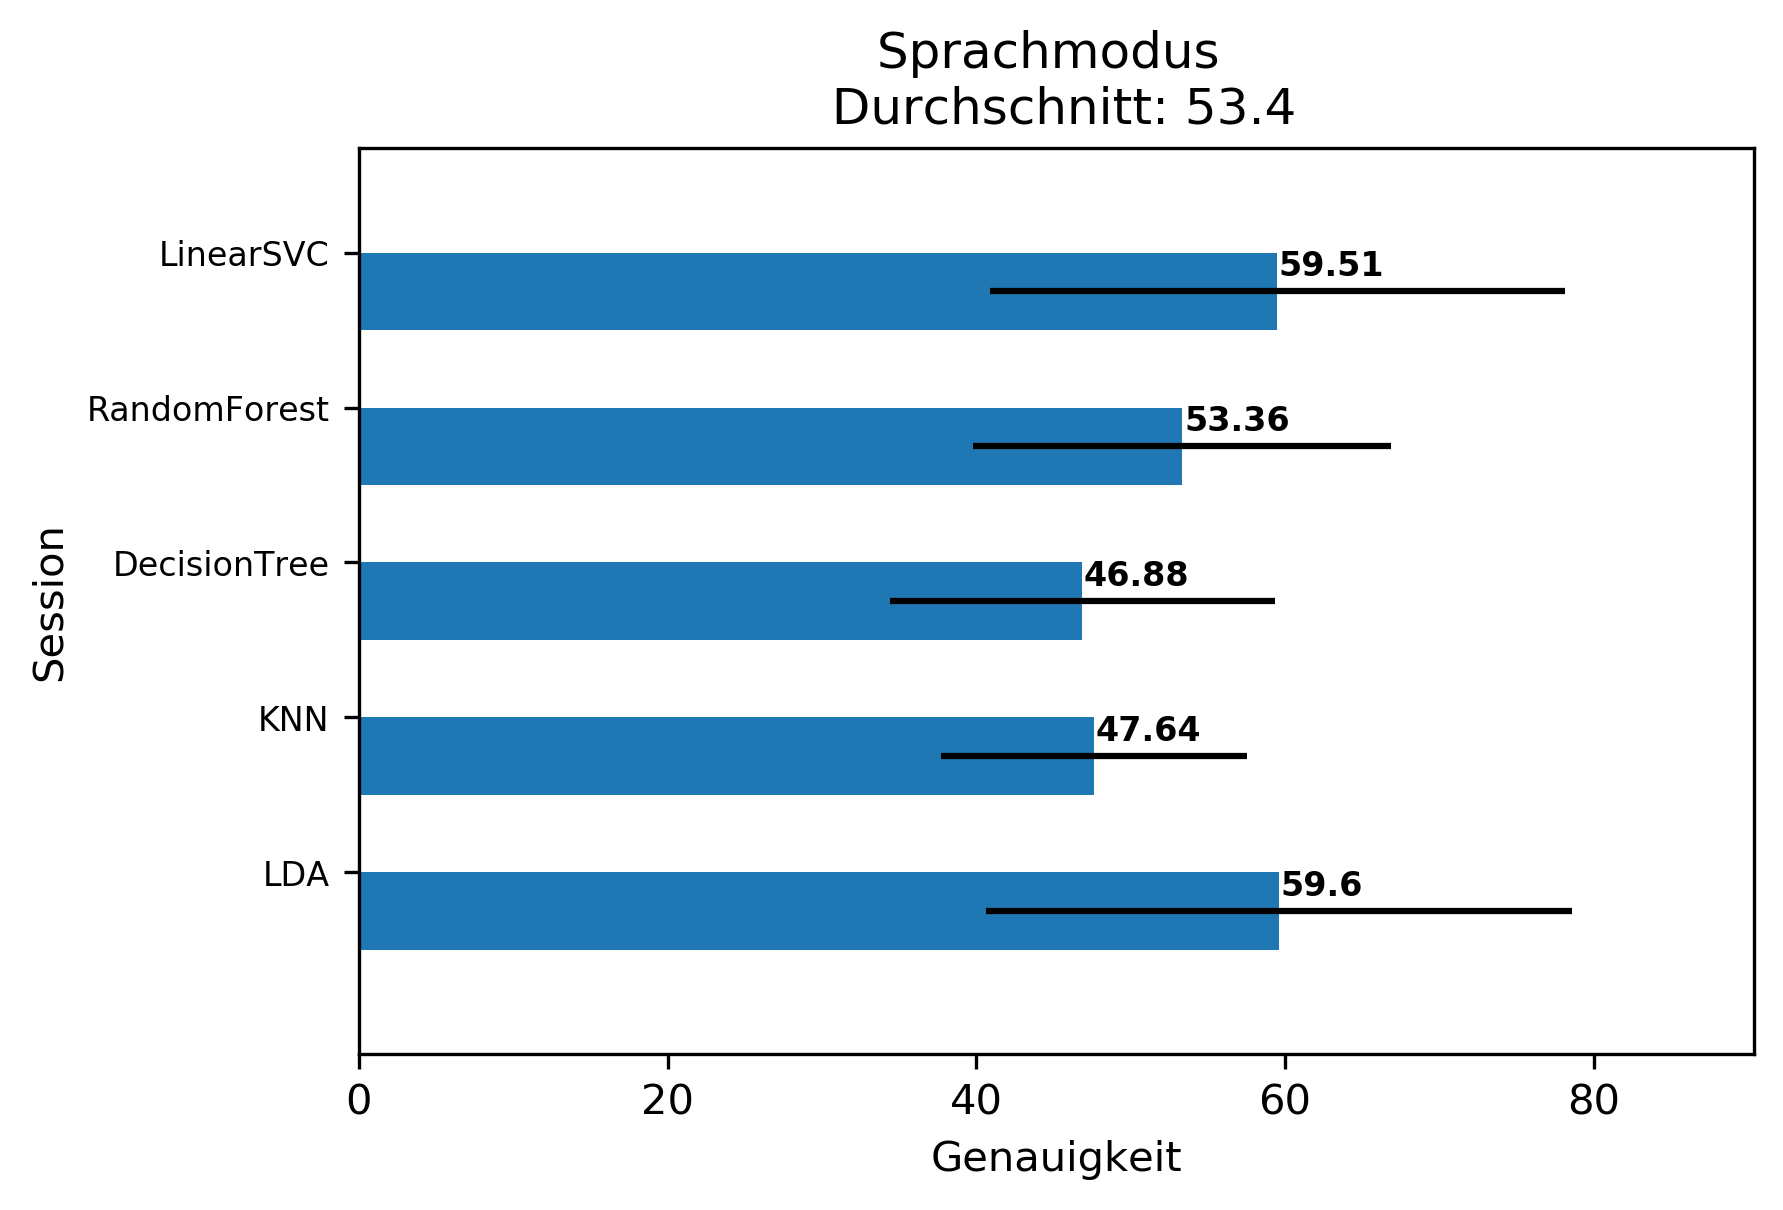
\includegraphics[width=100mm ,scale=0.6]{modeResultsSessionUnfiltered.png}
  \caption{Die durchschnittliche Genauigkeit, sowie die Standardabweichung der verschiedener Klassifikatoren bei der Erkennung des Sprachmodus. Hier werden die Daten aller Sprecher verwendet die mindestens 2 Sessions besitzen, also die Sprecher 1,2,4,7 und 8}
  \label{fig:mode1}
\end{figure}


\subsubsection{Sessions-Ungefiltert}

Hier werden die Genauigkeiten der verschiedenen Sessions von jedem Sprecher und der Durchschnittswert aller Sessions präsentiert. Die Resultate sind in der Tabelle \ref{tab:UnfModeSessions} zu sehen. Die höchste Genauigkeit ist in Session 2 von Sprecher 1 mit 86.67 Prozent, die niedrigste Genauigkeit ist Session 1 von Sprecher 4 mit 12 Prozent. Das passt zu den Resultaten der Sprechererkennung, in der diese Session ebenfalls die niedrigste Genauigkeit hatte.
Die höchste Durchschnittsgenauigkeit hat ebenfalls Sprecher 1 mit 74.67 Prozent. In \ref{fig:cnfus1} sieht man das die Klassifizierungen für silent in jeder Session über 90 Prozent genau sind.In Session 1 ist zudem die Genauigkeit für whisper mit 92 Prozent sehr hoch und in Session 2 ist mit 90 Prozent die Genauigkeit für audible sehr hoch.
Für Sprecher 7 (\ref{fig:cnfus3}) wurde in Session 1 alles als audible klassifiziert und in Session 2 alles als whisper klassifiziert. In Sprecher 4 (\ref{fig:cnfus2}) scheinen die Klassifizierungen einfach zufällig verteilt zu sein.

\begin{table}[H]
 \centering
 \caption{Genauigkeiten aller Sessions bei der Sprachmodus Erkennung mit ungefilterten Daten. }
\begin{tabular}{|c|c|}
\hline 
Session & Resultat in Prozent \\ 
\hline 
1001 & 65.33 \\ 
\hline 
1002 & 86.66\\ 
\hline 
1003 & 72 \\ 
\hline 
2001 & 66.67 \\ 
\hline 
2003 & 75.33 \\ 
\hline 
2004 & 43.33 \\  
\hline 
2005 & 85.33 \\ 
\hline 
2006 & 79.33 \\
\hline 
2007 & 78,66 \\
\hline 
2008 & 79,33 \\
\hline 
2009 & 60,66 \\
\hline 
2010 & 74 \\
\hline 
2012 & 78 \\
\hline 
2013 & 22,67 \\
\hline 
2028 & 52 \\
\hline 
2029 & 46,67 \\
\hline 
2031 & 63.22 \\
\hline 
2032 & 64 \\
\hline 
4001 & 12 \\ 
\hline 
4002 & 26,67 \\ 
\hline 
7001 & 34,67 \\ 
\hline 
7002 & 33,33 \\ 
\hline 
8002 & 58 \\ 
\hline 
8003 & 64 \\
\hline 
8010 & 42 \\
\hline 
8016 & 75,33 \\
\hline 
8017 & 42 \\
\hline 
8018 & 64 \\
\hline 
8019 & 58  \\ 
\hline 
\label{tab:UnfModeSessions} 
\end{tabular}
\end{table}


\begin{figure}[H]
\centering     %%% not \center
\subfigure[Session 1]{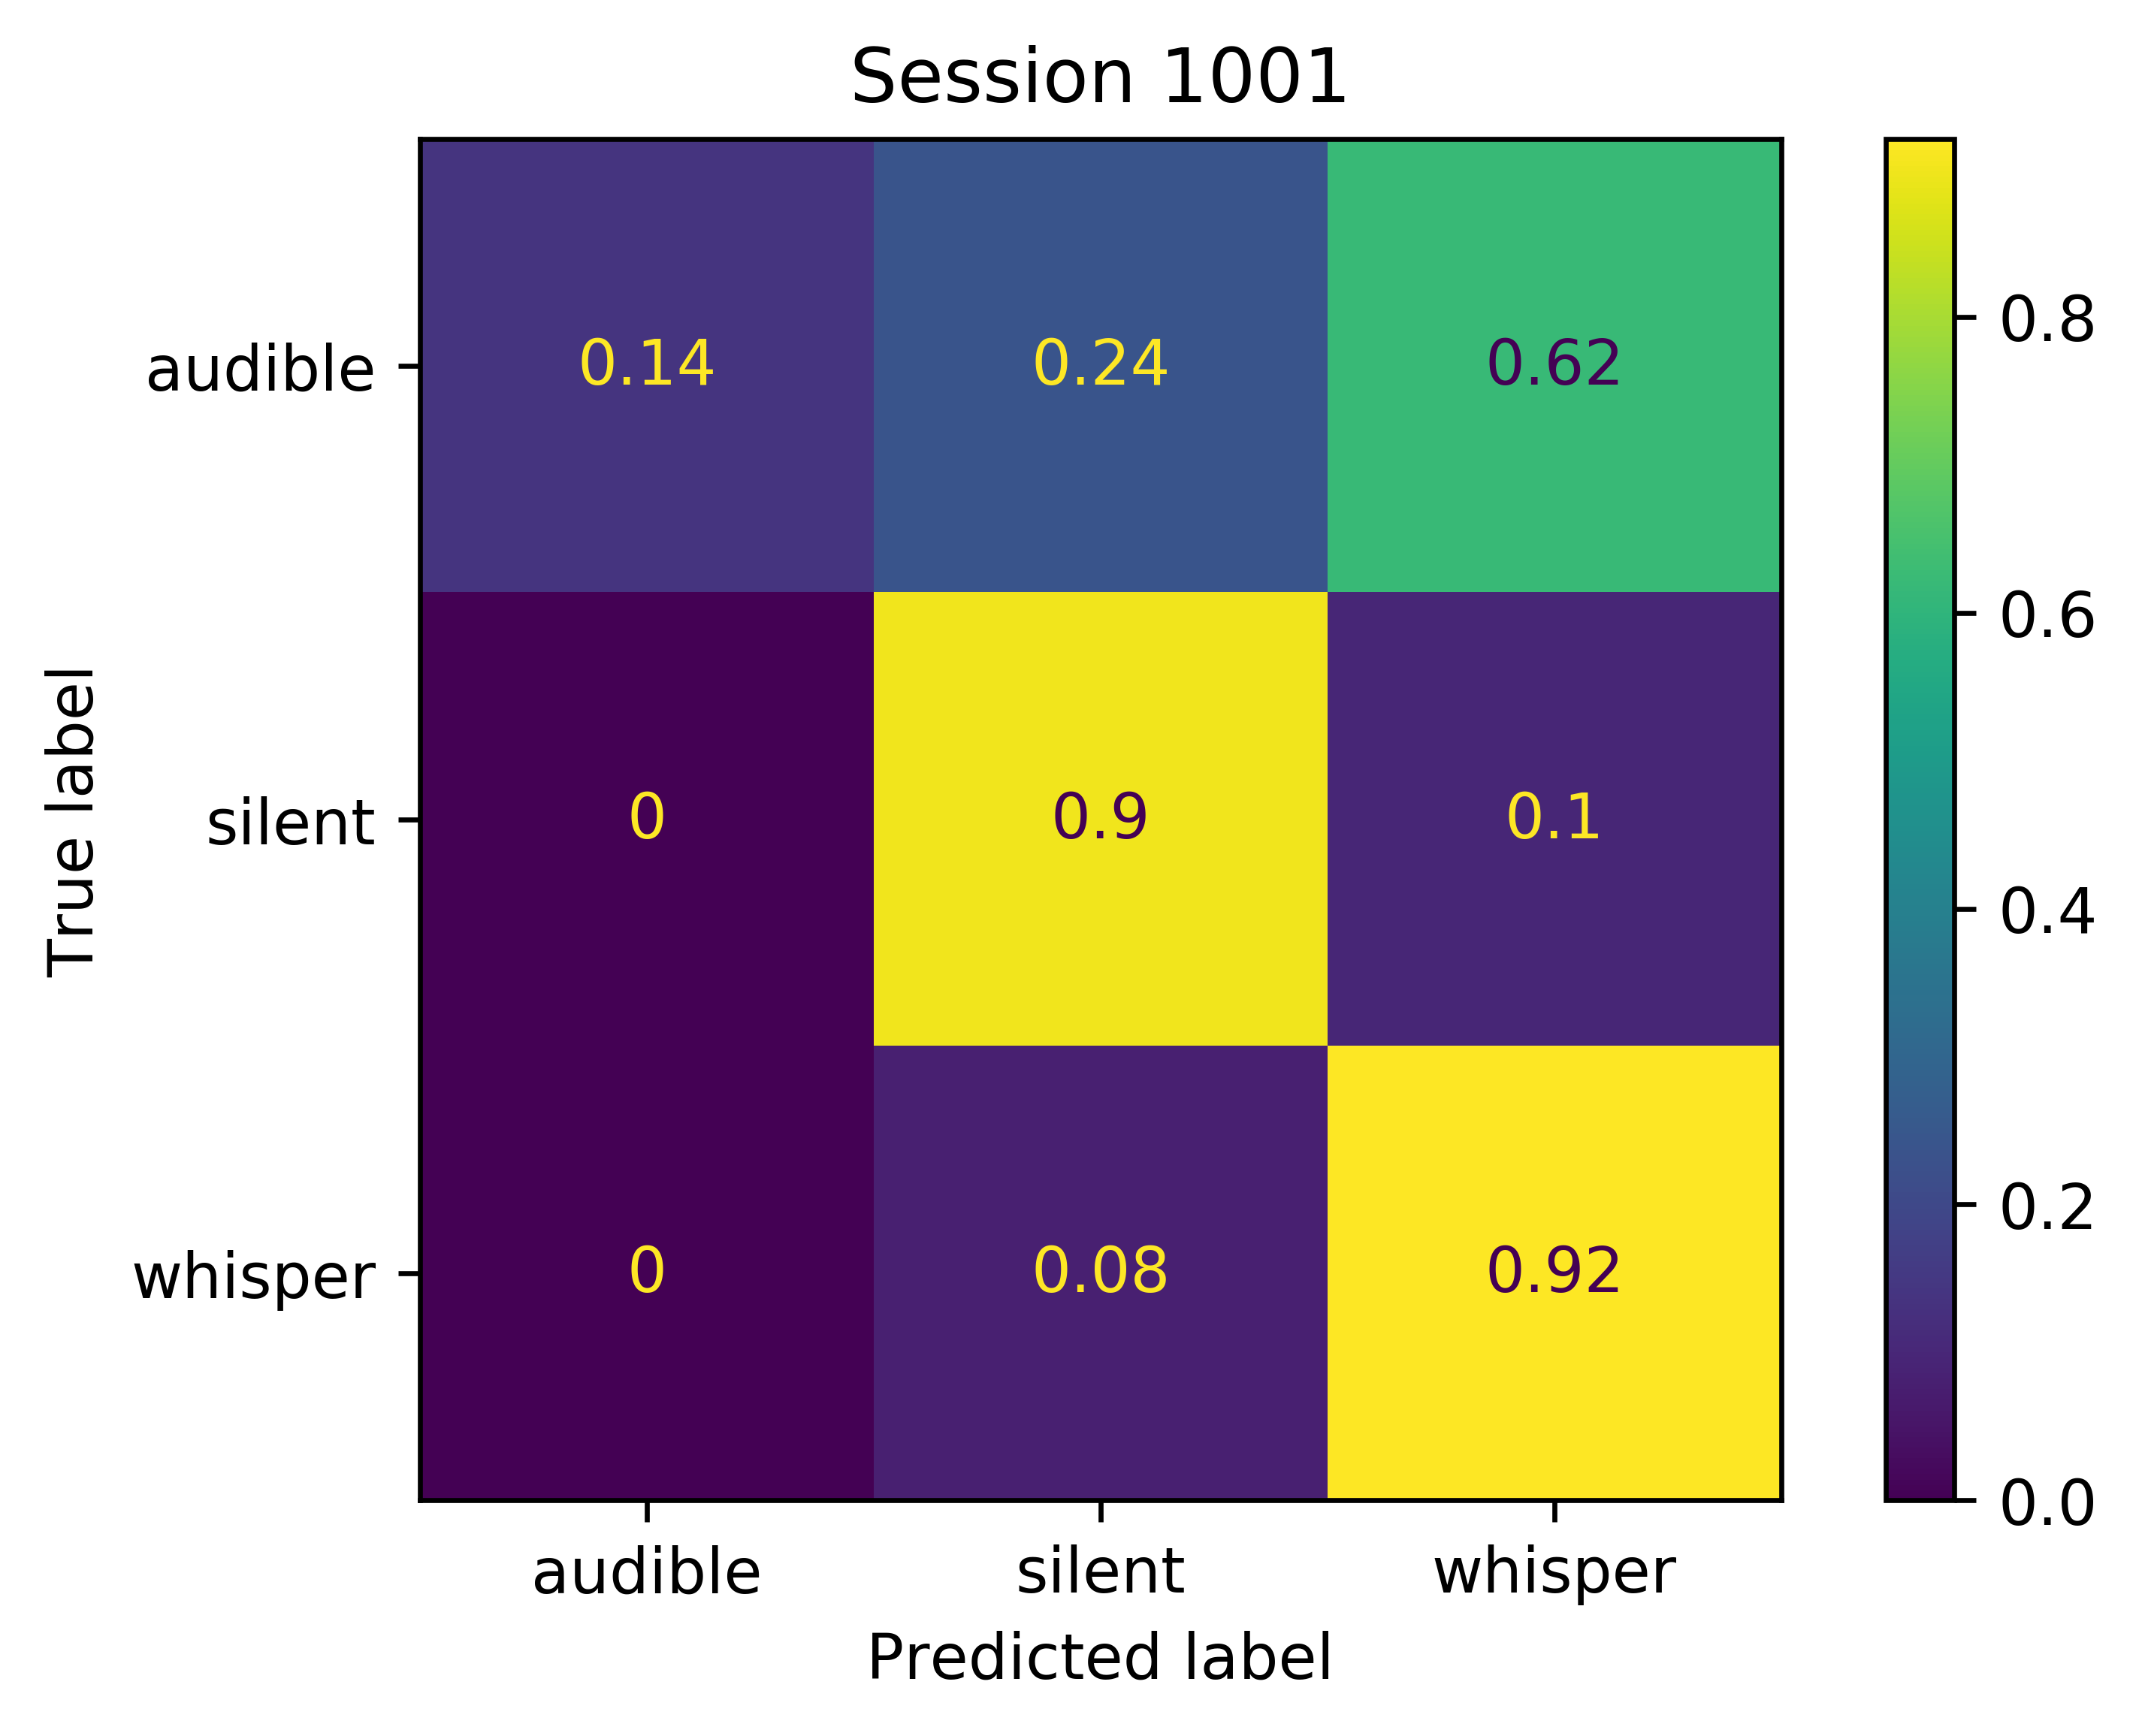
\includegraphics[width=70mm]{modeCrossSessionUnf/Session 1001_unf.png}}
\subfigure[Session 2]{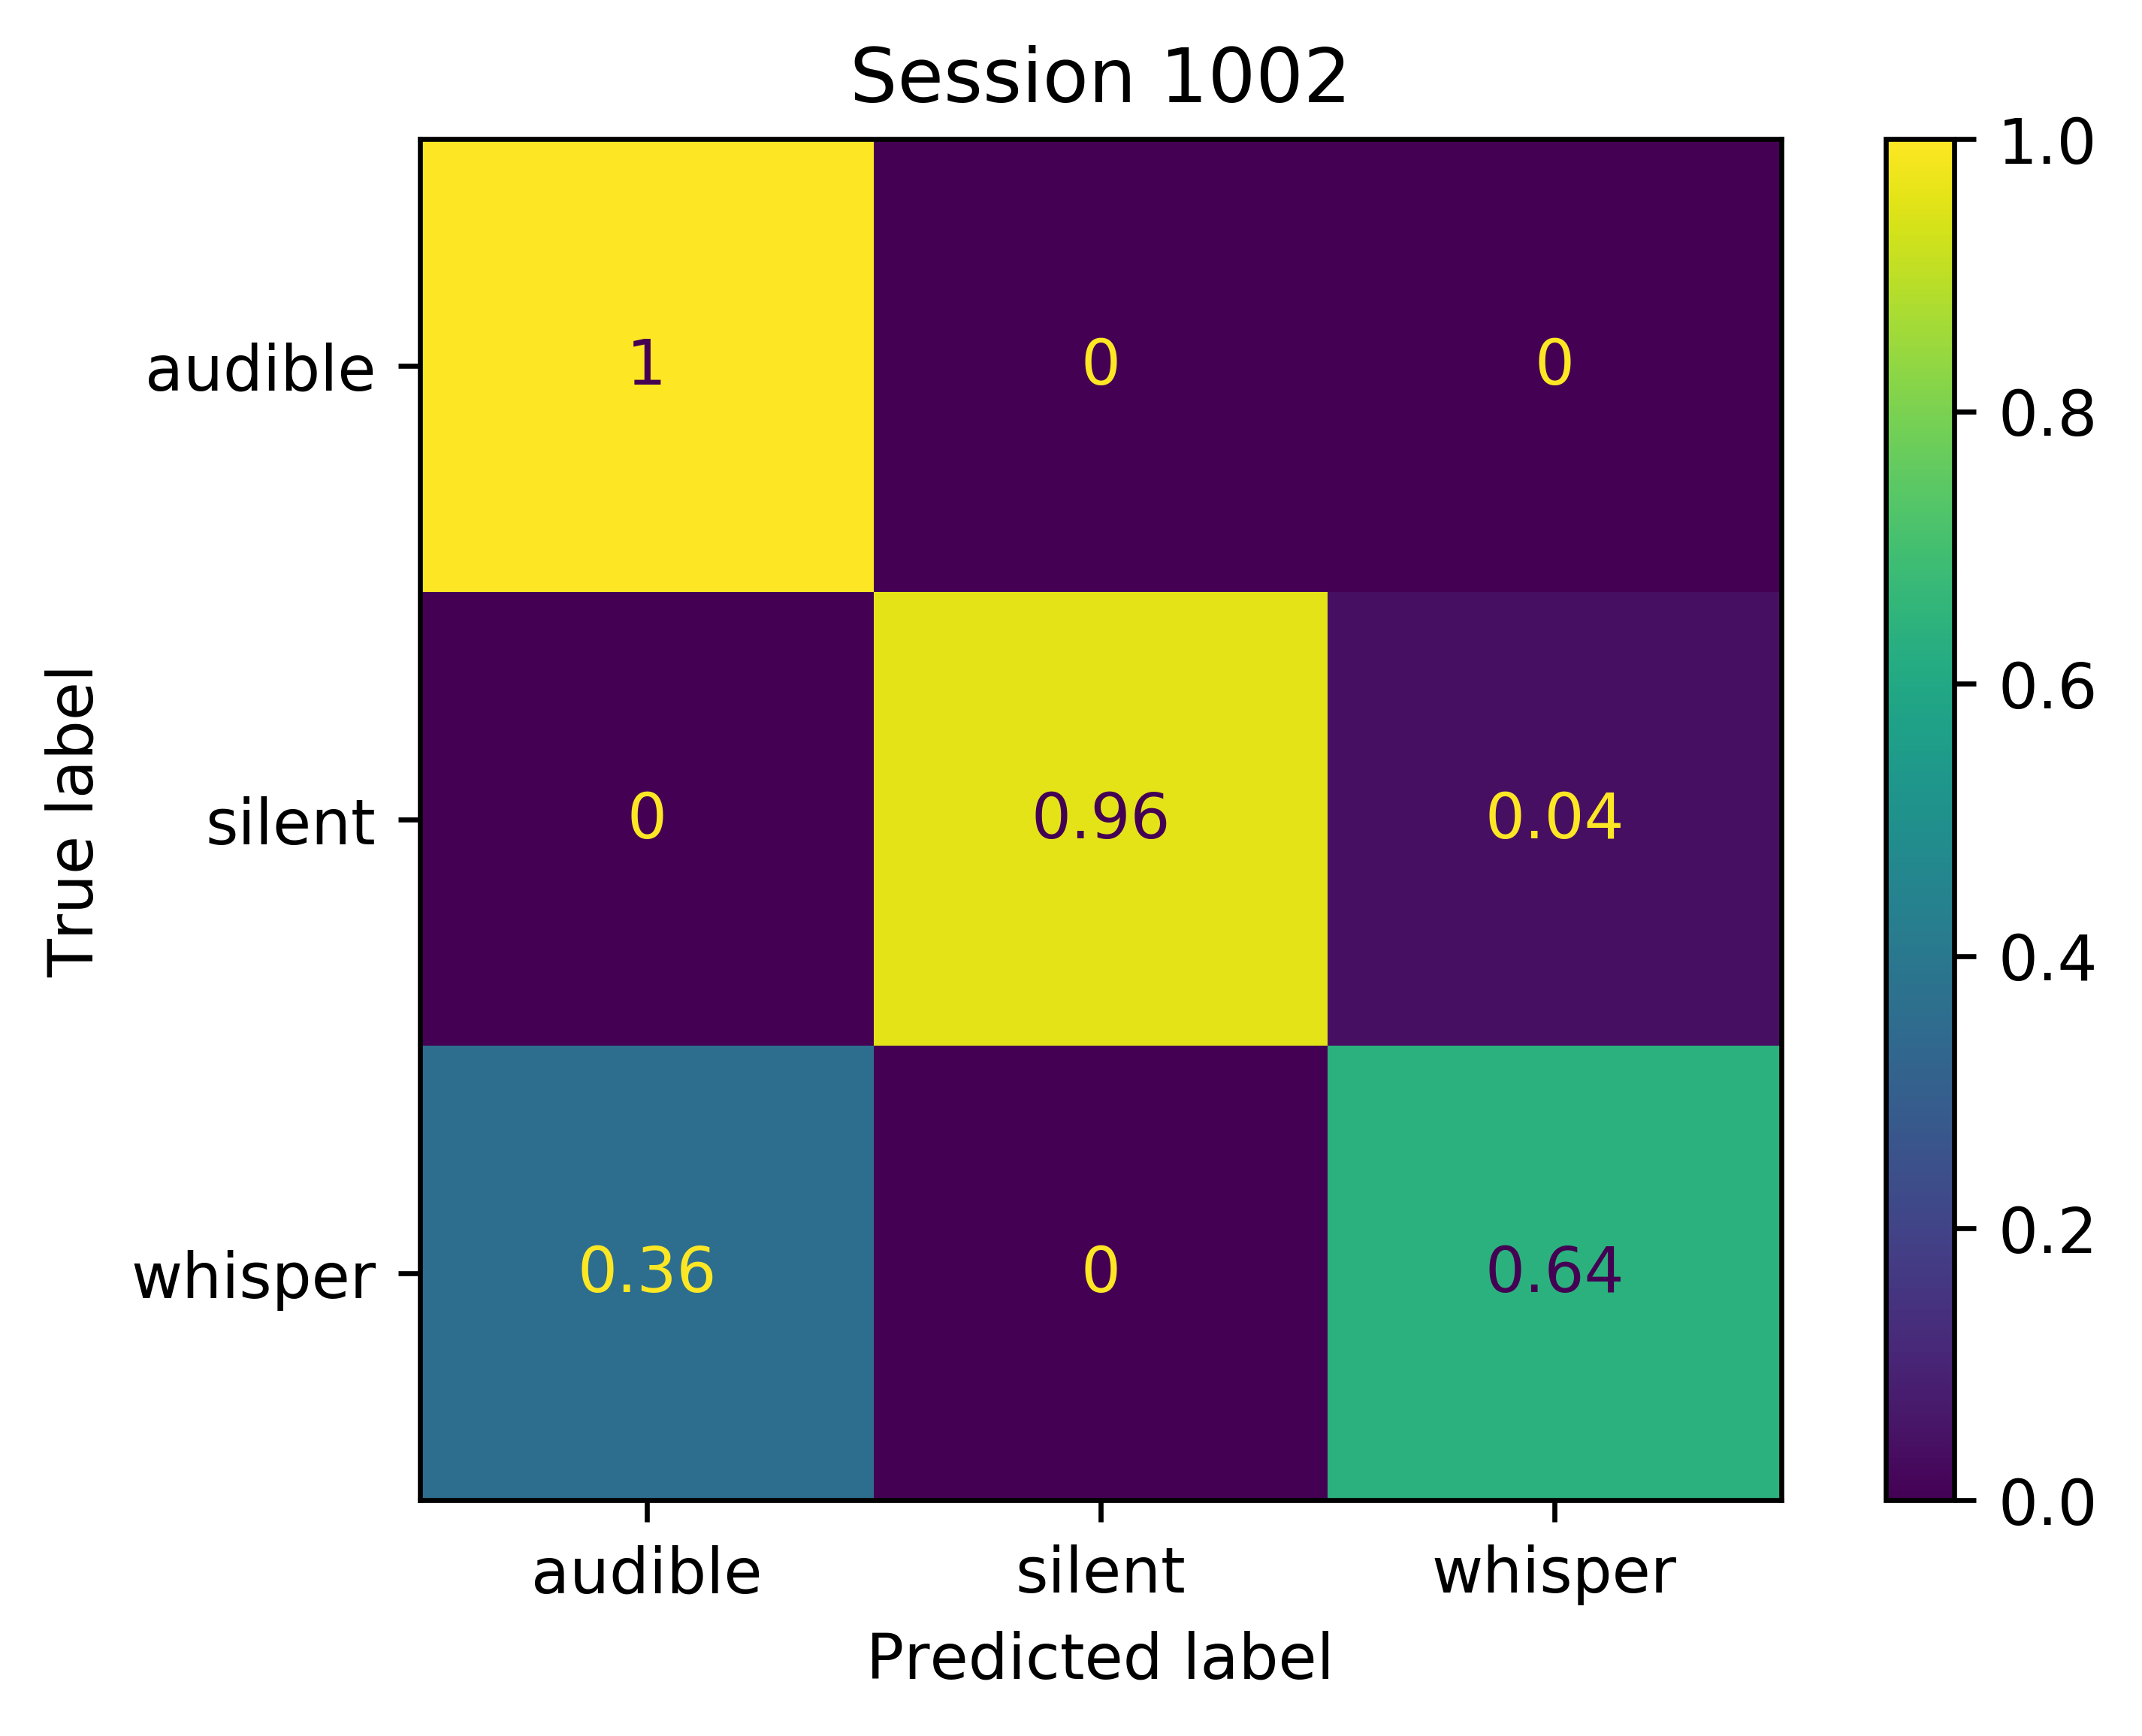
\includegraphics[width=70mm]{modeCrossSessionUnf/Session 1002_unf.png}}
\subfigure[Session 3]{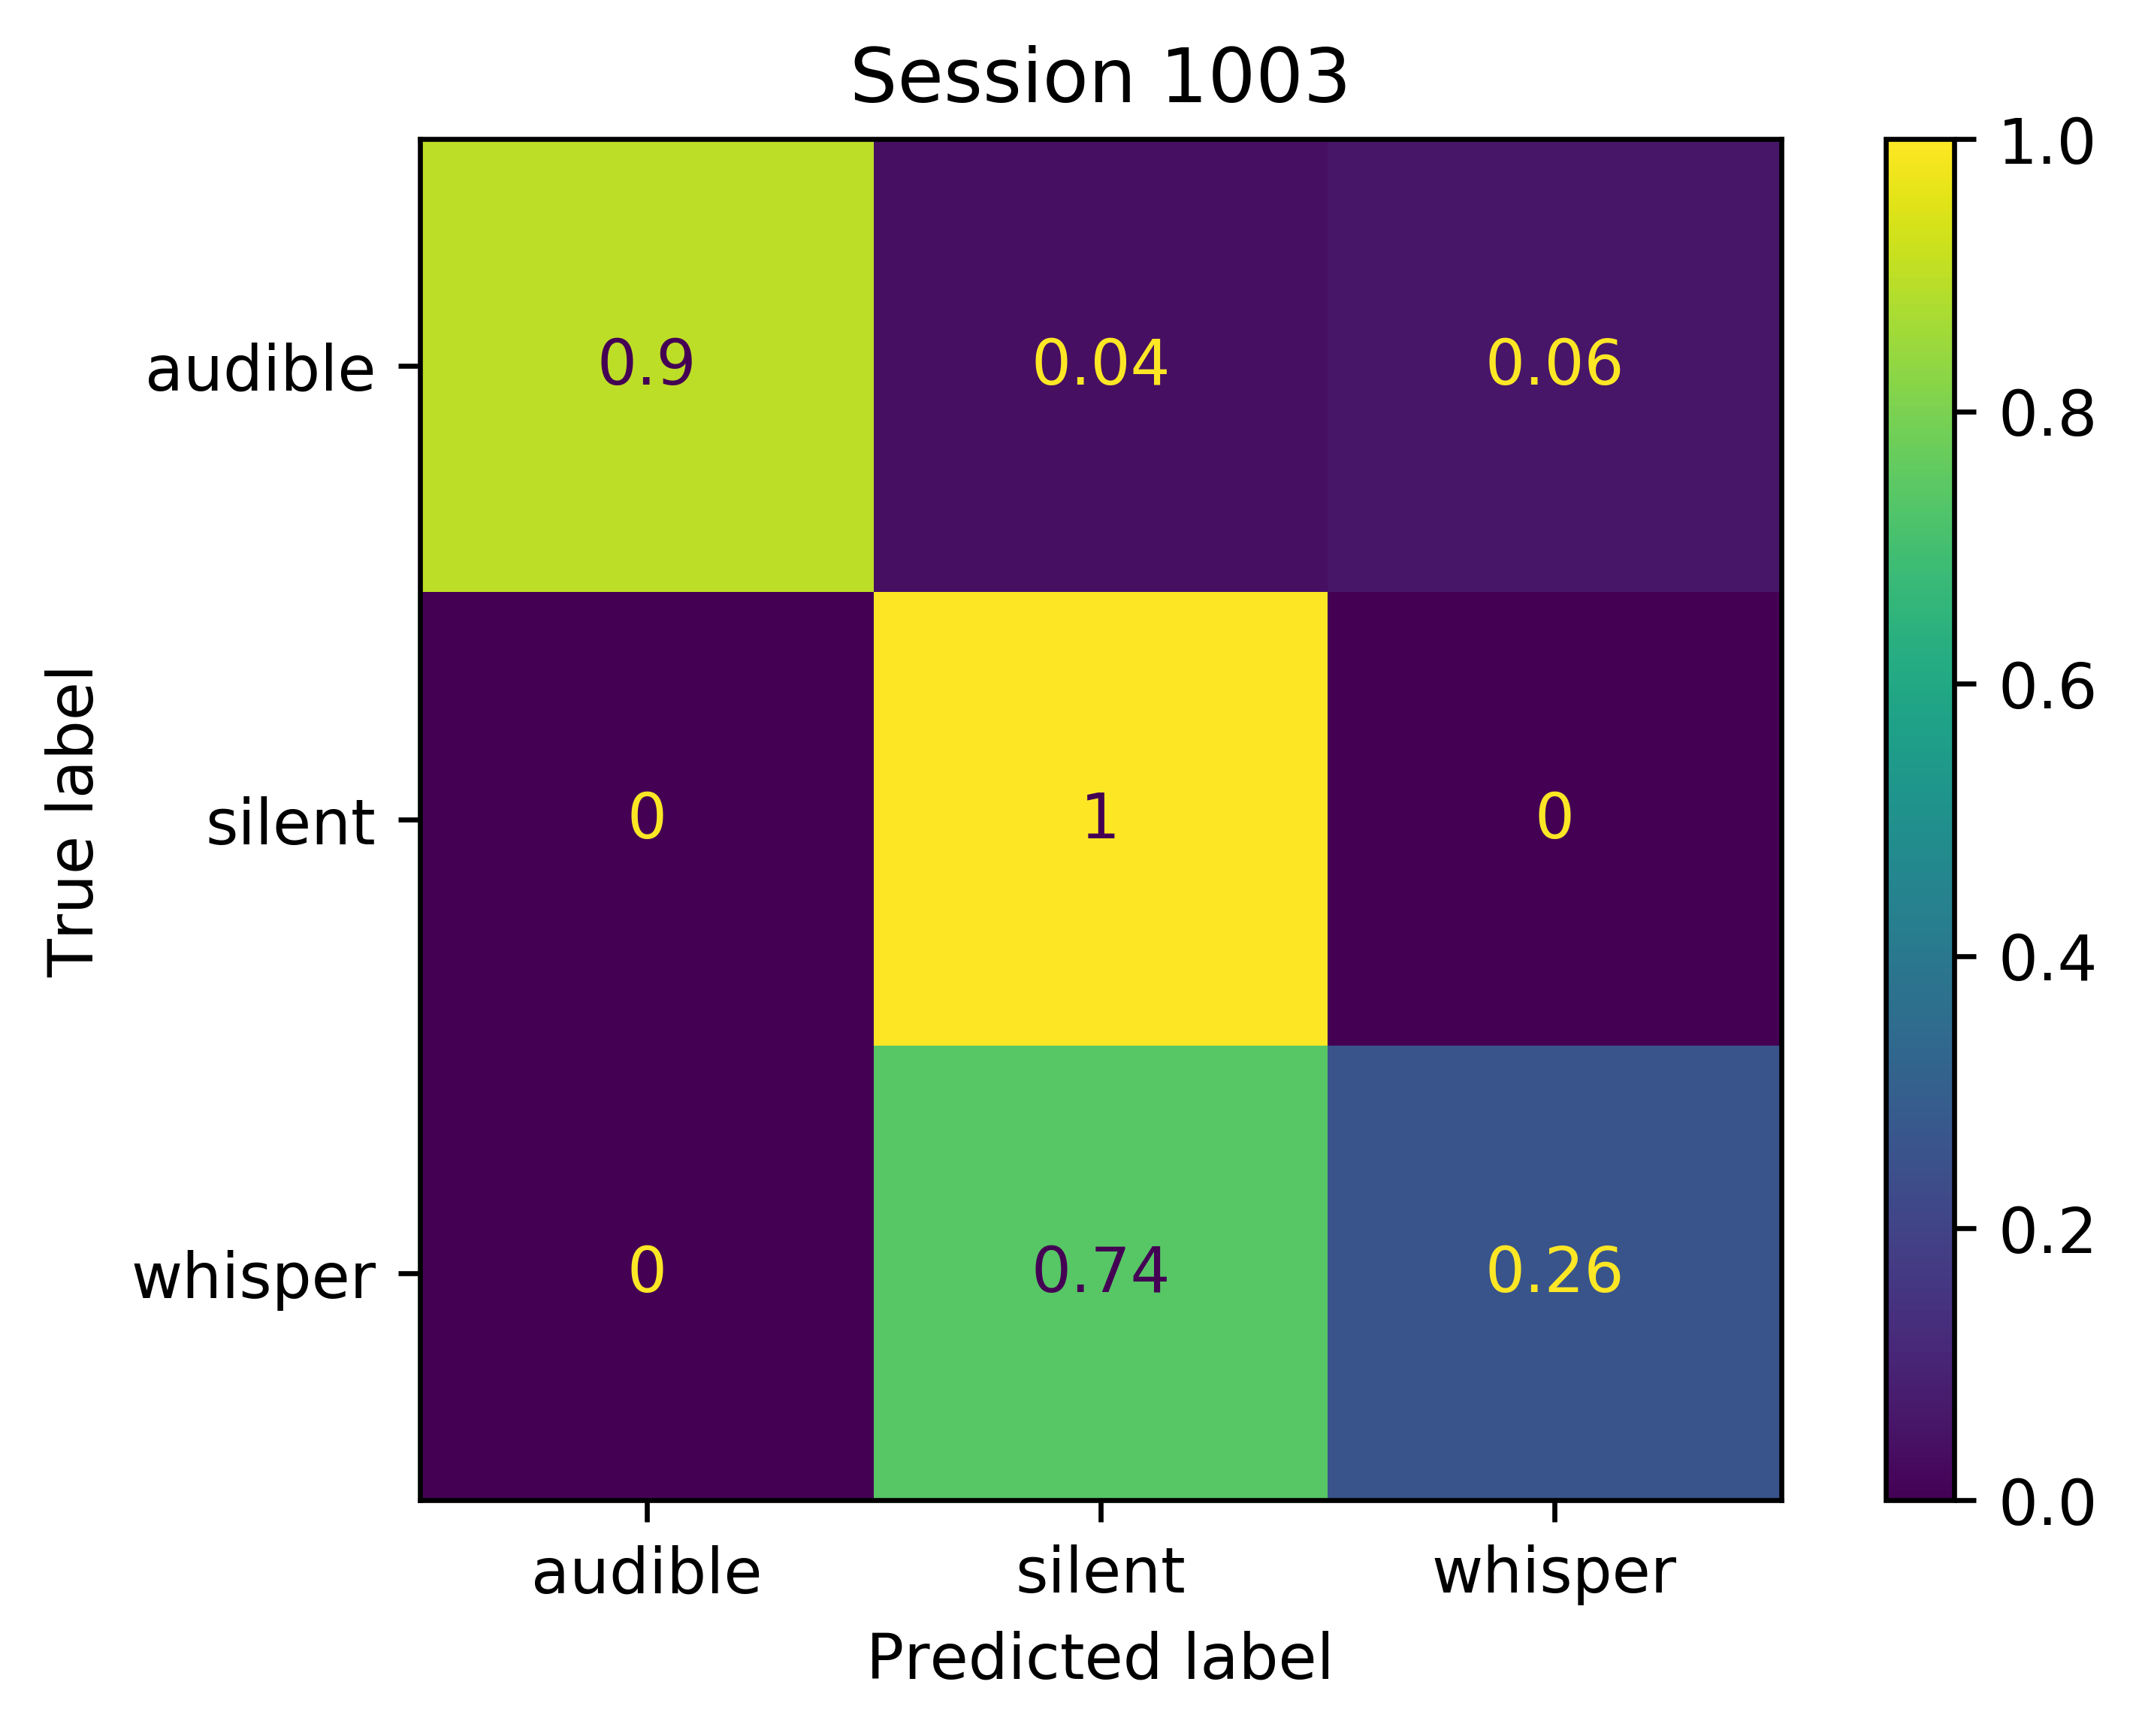
\includegraphics[width=70mm]{modeCrossSessionUnf/Session 1003_unf.png}}
\caption{Erkennungsraten von Sprecher 1 für die Vorhersage des Sprachmodus mit ungefilterten Daten.}
\label{fig:cnfus1}
\end{figure}


\begin{figure}[H]
\centering     %%% not \center
\subfigure[Sprecher 4]{\label{fig:cnfus2}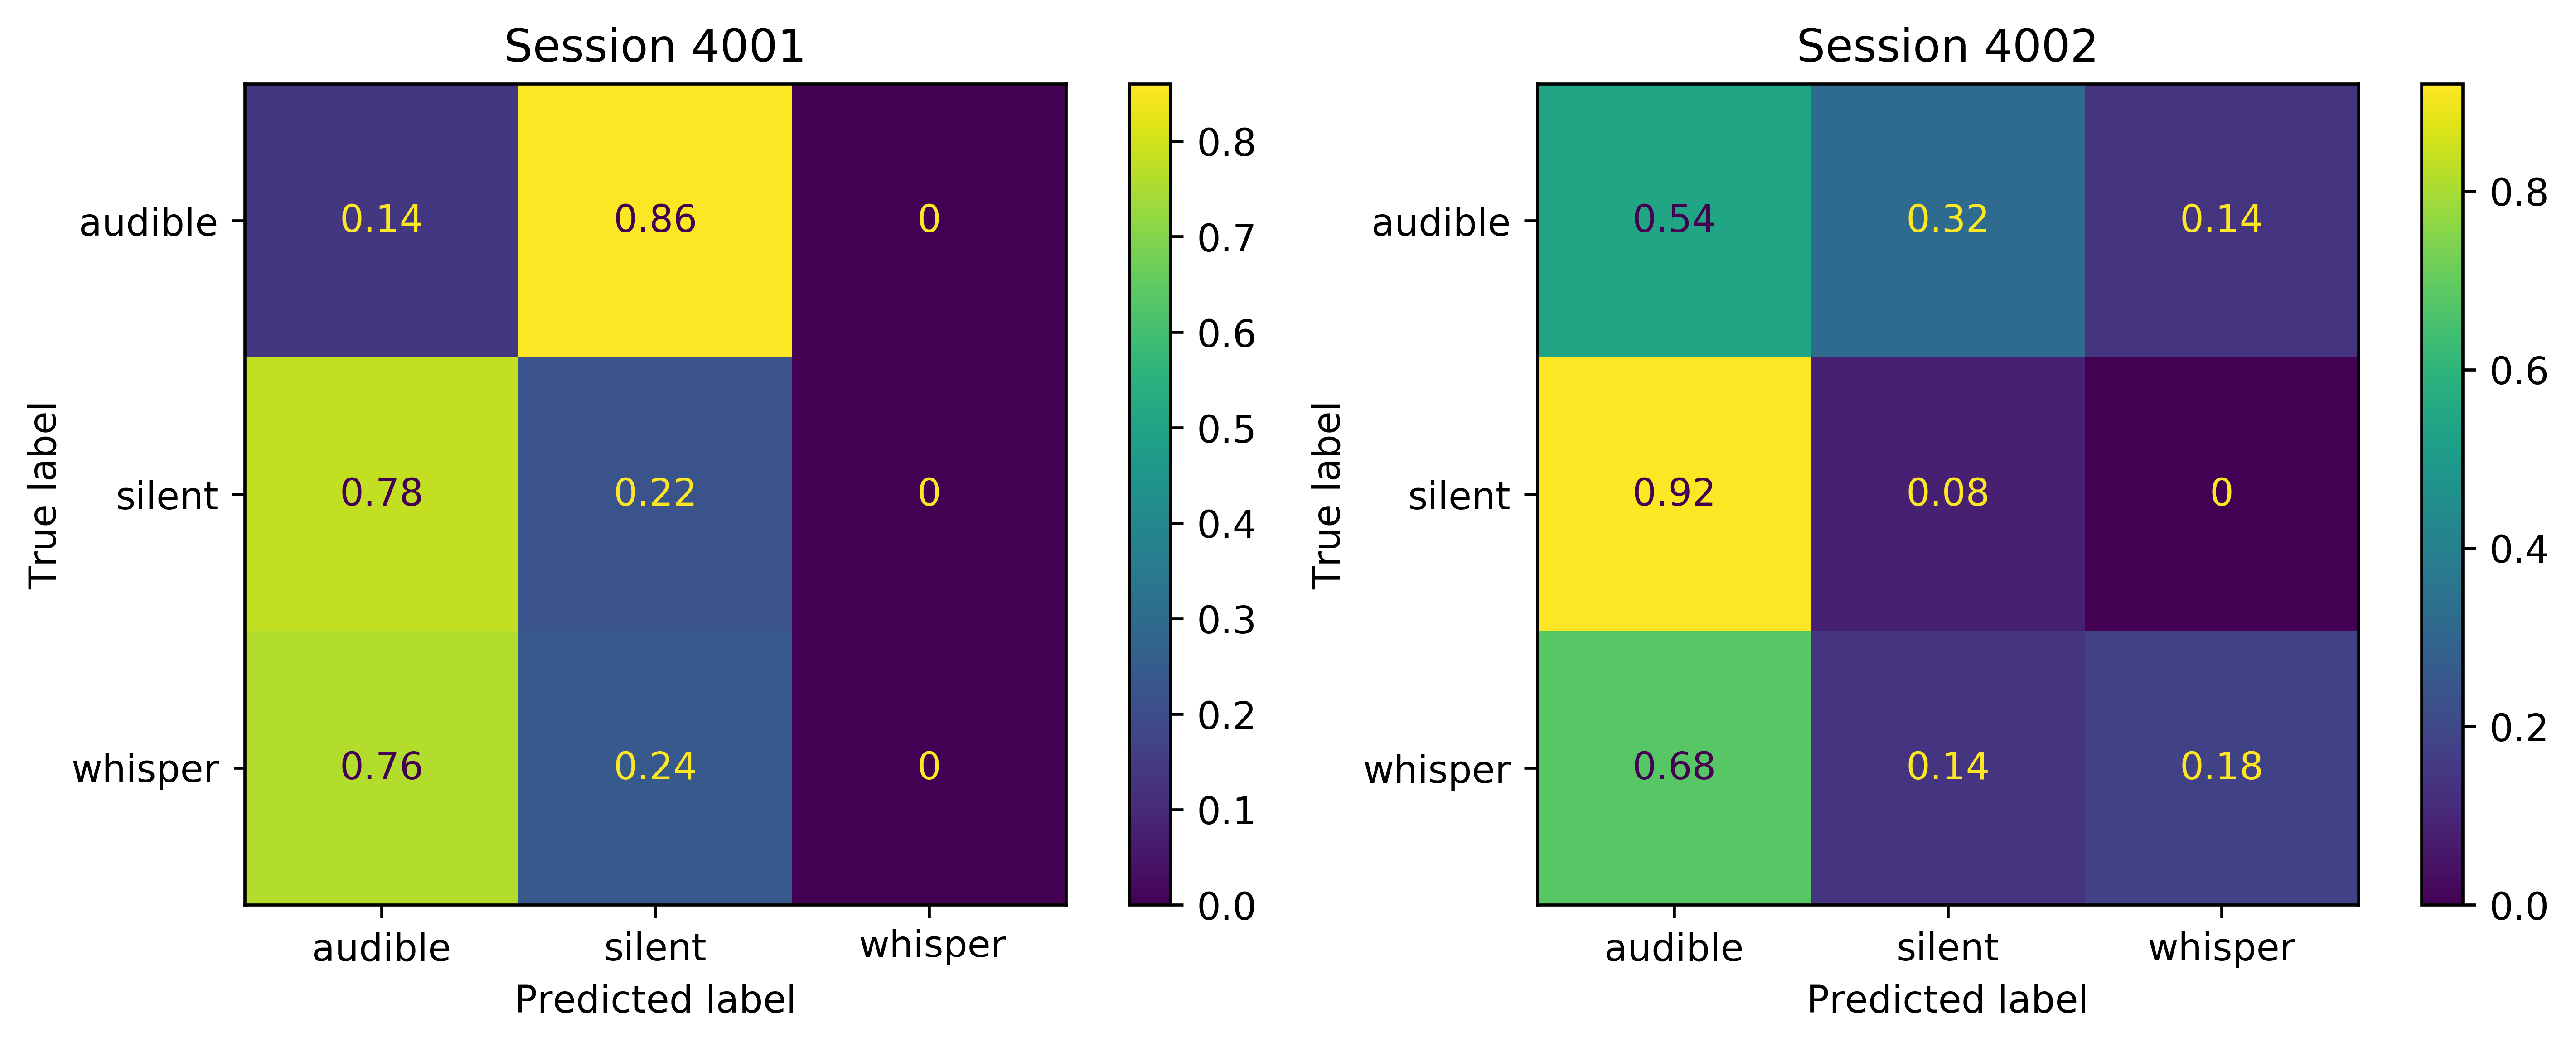
\includegraphics[width=\linewidth]{modeConfMatUser4SessionUnf.png}}
\subfigure[Sprecher 7]{\label{fig:cnfus3}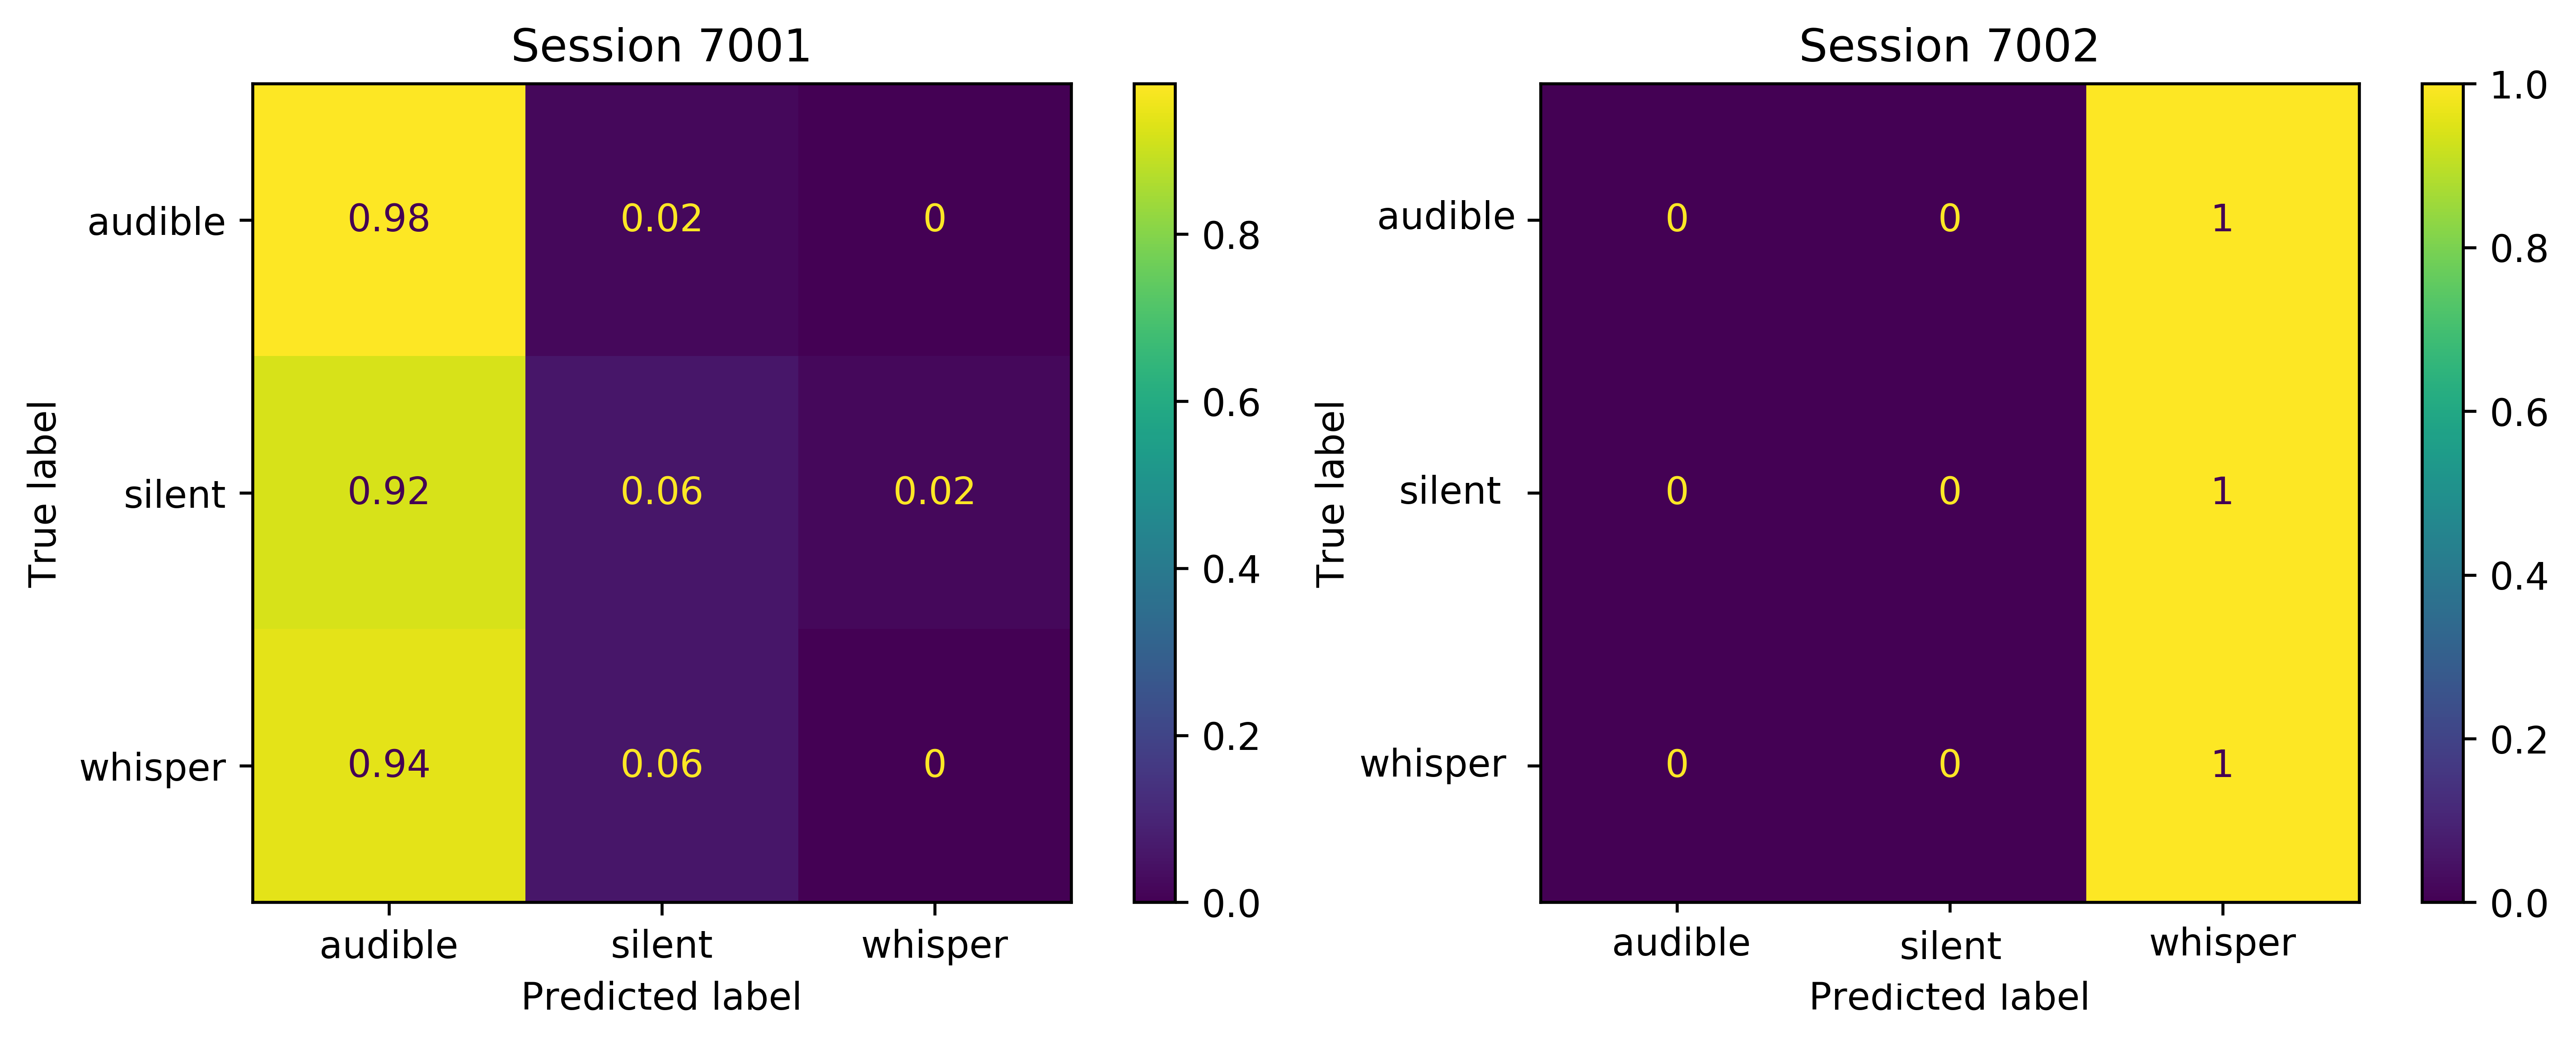
\includegraphics[width=\linewidth]{modeConfMatUser7SessionUnf.png}}
\caption{Die Erkennungsraten der Sprecher 4 und 7 für die Vorhersage des Sprachmodus mit ungefilterten Daten.}
\end{figure}
\clearpage

\subsubsection{Filtered}
Hier(\ref{fig:mode2}) wurde einen Bandpassfilter angewendet. Dieser filtert alles unter 10Hz und alles über 200Hz. Diese Filter Grenzen wurden mit Absprache meiner Tutoren gewählt und sollen unwichtige Artefakte und Hintergrundrauschen rausfiltern, um damit die Genauigkeit zu erhöhen. Es ist eine ähnliche Verteilung der Genauigkeit wie in (\ref{fig:mode1}) zu betrachten wobei der Lda, der Randomforest sowie der LinerSVC die höchsten Werte vorweisen. Hier hat wieder der LDA-Klassifikator mit 55.04 Prozent die höchste Genauigkeit. Der KNN-Klassifikator hat die niedrigste Genauigkeit mit 41.12 Prozent. Es lässt sich eine allgemein niedrigere Genauigkeit als bei der ungefilterten Variante in \ref{fig:mode1} beobachten.

\begin{figure}[H]
  \centering
  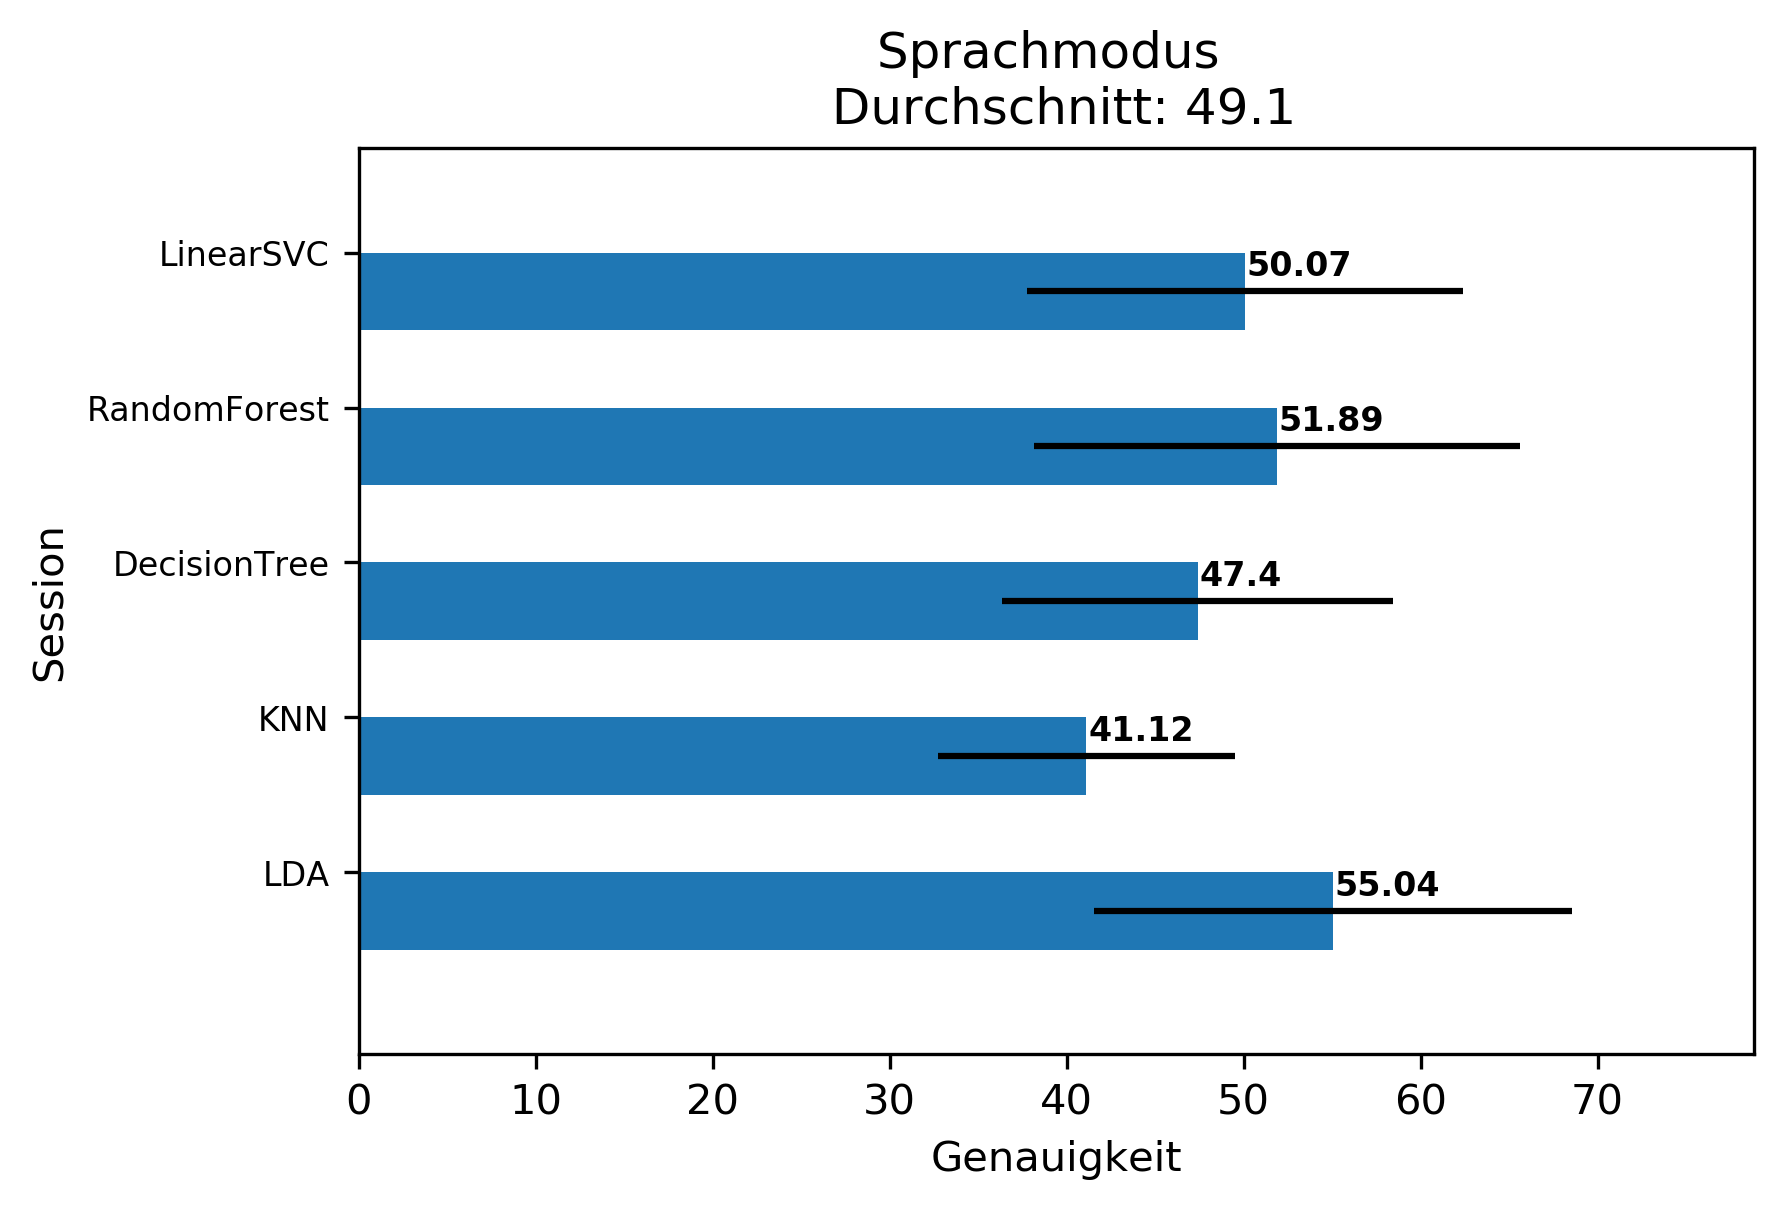
\includegraphics[width=100mm ,scale=0.6]{modeResultsSession10too200hz .png}
  \caption{Die durchschnittliche Genauigkeit, sowie die Standardabweichung verschiedener Klassifikatoren bei der Erkennung des Sprachmodus. Hier werden die Daten aller Sprecher verwendet die mindestens 2 Sessions besitzen, also die Sprecher 1,2,4,7 und 8. Zudem wurde hier ein Bandpassfilter von 10 bis 200Hz verwendet.}
  \label{fig:mode2}
\end{figure}

\clearpage

\subsubsection{Sessions-Filtered}
Hier wurde sich die Genauigkeiten der verschiedenen Sessions von jedem Sprecher und der Durchschnittswert aller Sessions angeguckt (\ref{tab:FiltModeSessions}). Die höchsten erreichte Genauigkeit war in Session 3 von Sprecher 1 mit 84.67 Prozent die niedrigste Genauigkeit ist Session 1 von Sprecher 4 mit 18.67 Prozent. Das passt zu den Resultaten der Sprechererkennung in der diese Session ebenfalls die niedrigste Genauigkeit hatte.
Die höchste Durchschnittsgenauigkeit hat Sprecher 8 mit 74.43 Prozent.

\begin{table}[H]
 \centering
 \caption{Genauigkeiten aller Sessions bei der Sprachmodus Erkennung mit gefilterten Daten. }
\begin{tabular}{|c|c|}
\hline 
Session & Resultat in Prozent \\ 
\hline 
1001 & 84.67 \\ 
\hline 
1002 & 75.33\\ 
\hline 
1003 & 63.33 \\ 
\hline 
2001 & 66\\ 
\hline 
2003 & 66 \\ 
\hline 
2004 & 42.67 \\  
\hline 
2005 & 68.67 \\ 
\hline 
2006 & 69.33 \\
\hline 
2007 & 66 \\
\hline 
2008 & 61.33 \\
\hline 
2009 & 56 \\
\hline 
2010 & 62.67 \\
\hline 
2012 & 62 \\
\hline 
2013 & 34.67 \\
\hline 
2028 & 43.33 \\
\hline 
2029 & 48 \\
\hline 
2031 & 34.67 \\
\hline 
2032 & 42,67 \\
\hline 
4001 & 41,33 \\ 
\hline 
4002 & 18,67 \\ 
\hline 
7001 & 36 \\ 
\hline 
7002 & 46,67\\ 
\hline 
8002 & 62,67 \\ 
\hline 
8003 & 54,67 \\
\hline 
8010 & 58,67 \\
\hline 
8016 & 64 \\
\hline 
8017 & 51,33 \\
\hline 
8018 & 61,33 \\
\hline 
8019 & 66,61 \\ 
\hline   
\label{tab:FiltModeSessions} 
\end{tabular}
\end{table}
 
 
\clearpage
\subsubsection{Frequenzbänder}
In \cite{Avan2001-BOX} wird die Verbindung zwischen verschiedenen Frequenzbändern in der EMG-Aufnahme und die Verbindung zu verschiedenen Muskelgruppen dargestellt. In diesem Teil wurde kontrolliert, ob es ein erkennbares Frequenzband gibt welches bessere Resultate vorzeigt. Damit wäre nämlich bewiesen, dass ein bestimmter Muskel für die Vorhersage des Sprachmodi größere Wichtigkeit ist als die anderen. Das Signal wurde in Frequenzbänder der Größe 10 aufgeteilt und ihre Genauigkeit in den verschiedenen Frequenzbereichen betrachtet. Hier wurde ein LDA verwendet. Die Resultate sind in \ref{fig:mode3} zu sehen. Es ist eine gleichmäßige Verteilung von Genauigkeiten im 46–51 Prozent Bereich zu beobachten mit den niedrigsten Werten an den beiden Enden mit 34.98 Prozent im 290-300Hz Bereich und 41.22 Prozent im 0–10 Hz Bereich. Der höchste Wert ist im 10-20Hz Bereich mit 52.49 Prozent zu beobachten. Im 260-270Hz Bereich lässt sich jedoch ebenfalls eine Genauigkeit von 52.11 Prozent beobachten. Aufgrund der nur sehr kleine Unterschiede zwischen den verschiedenen Frequenzbändern lässt sich allerdings kein Frequenzbereich als der beste Frequenzbereich eingrenzen. Die besten Frequenzbereiche sind die Bereiche von 10-40Hz 70-130Hz und 260-290Hz eingrenzen.
\begin{figure}[H]
  
  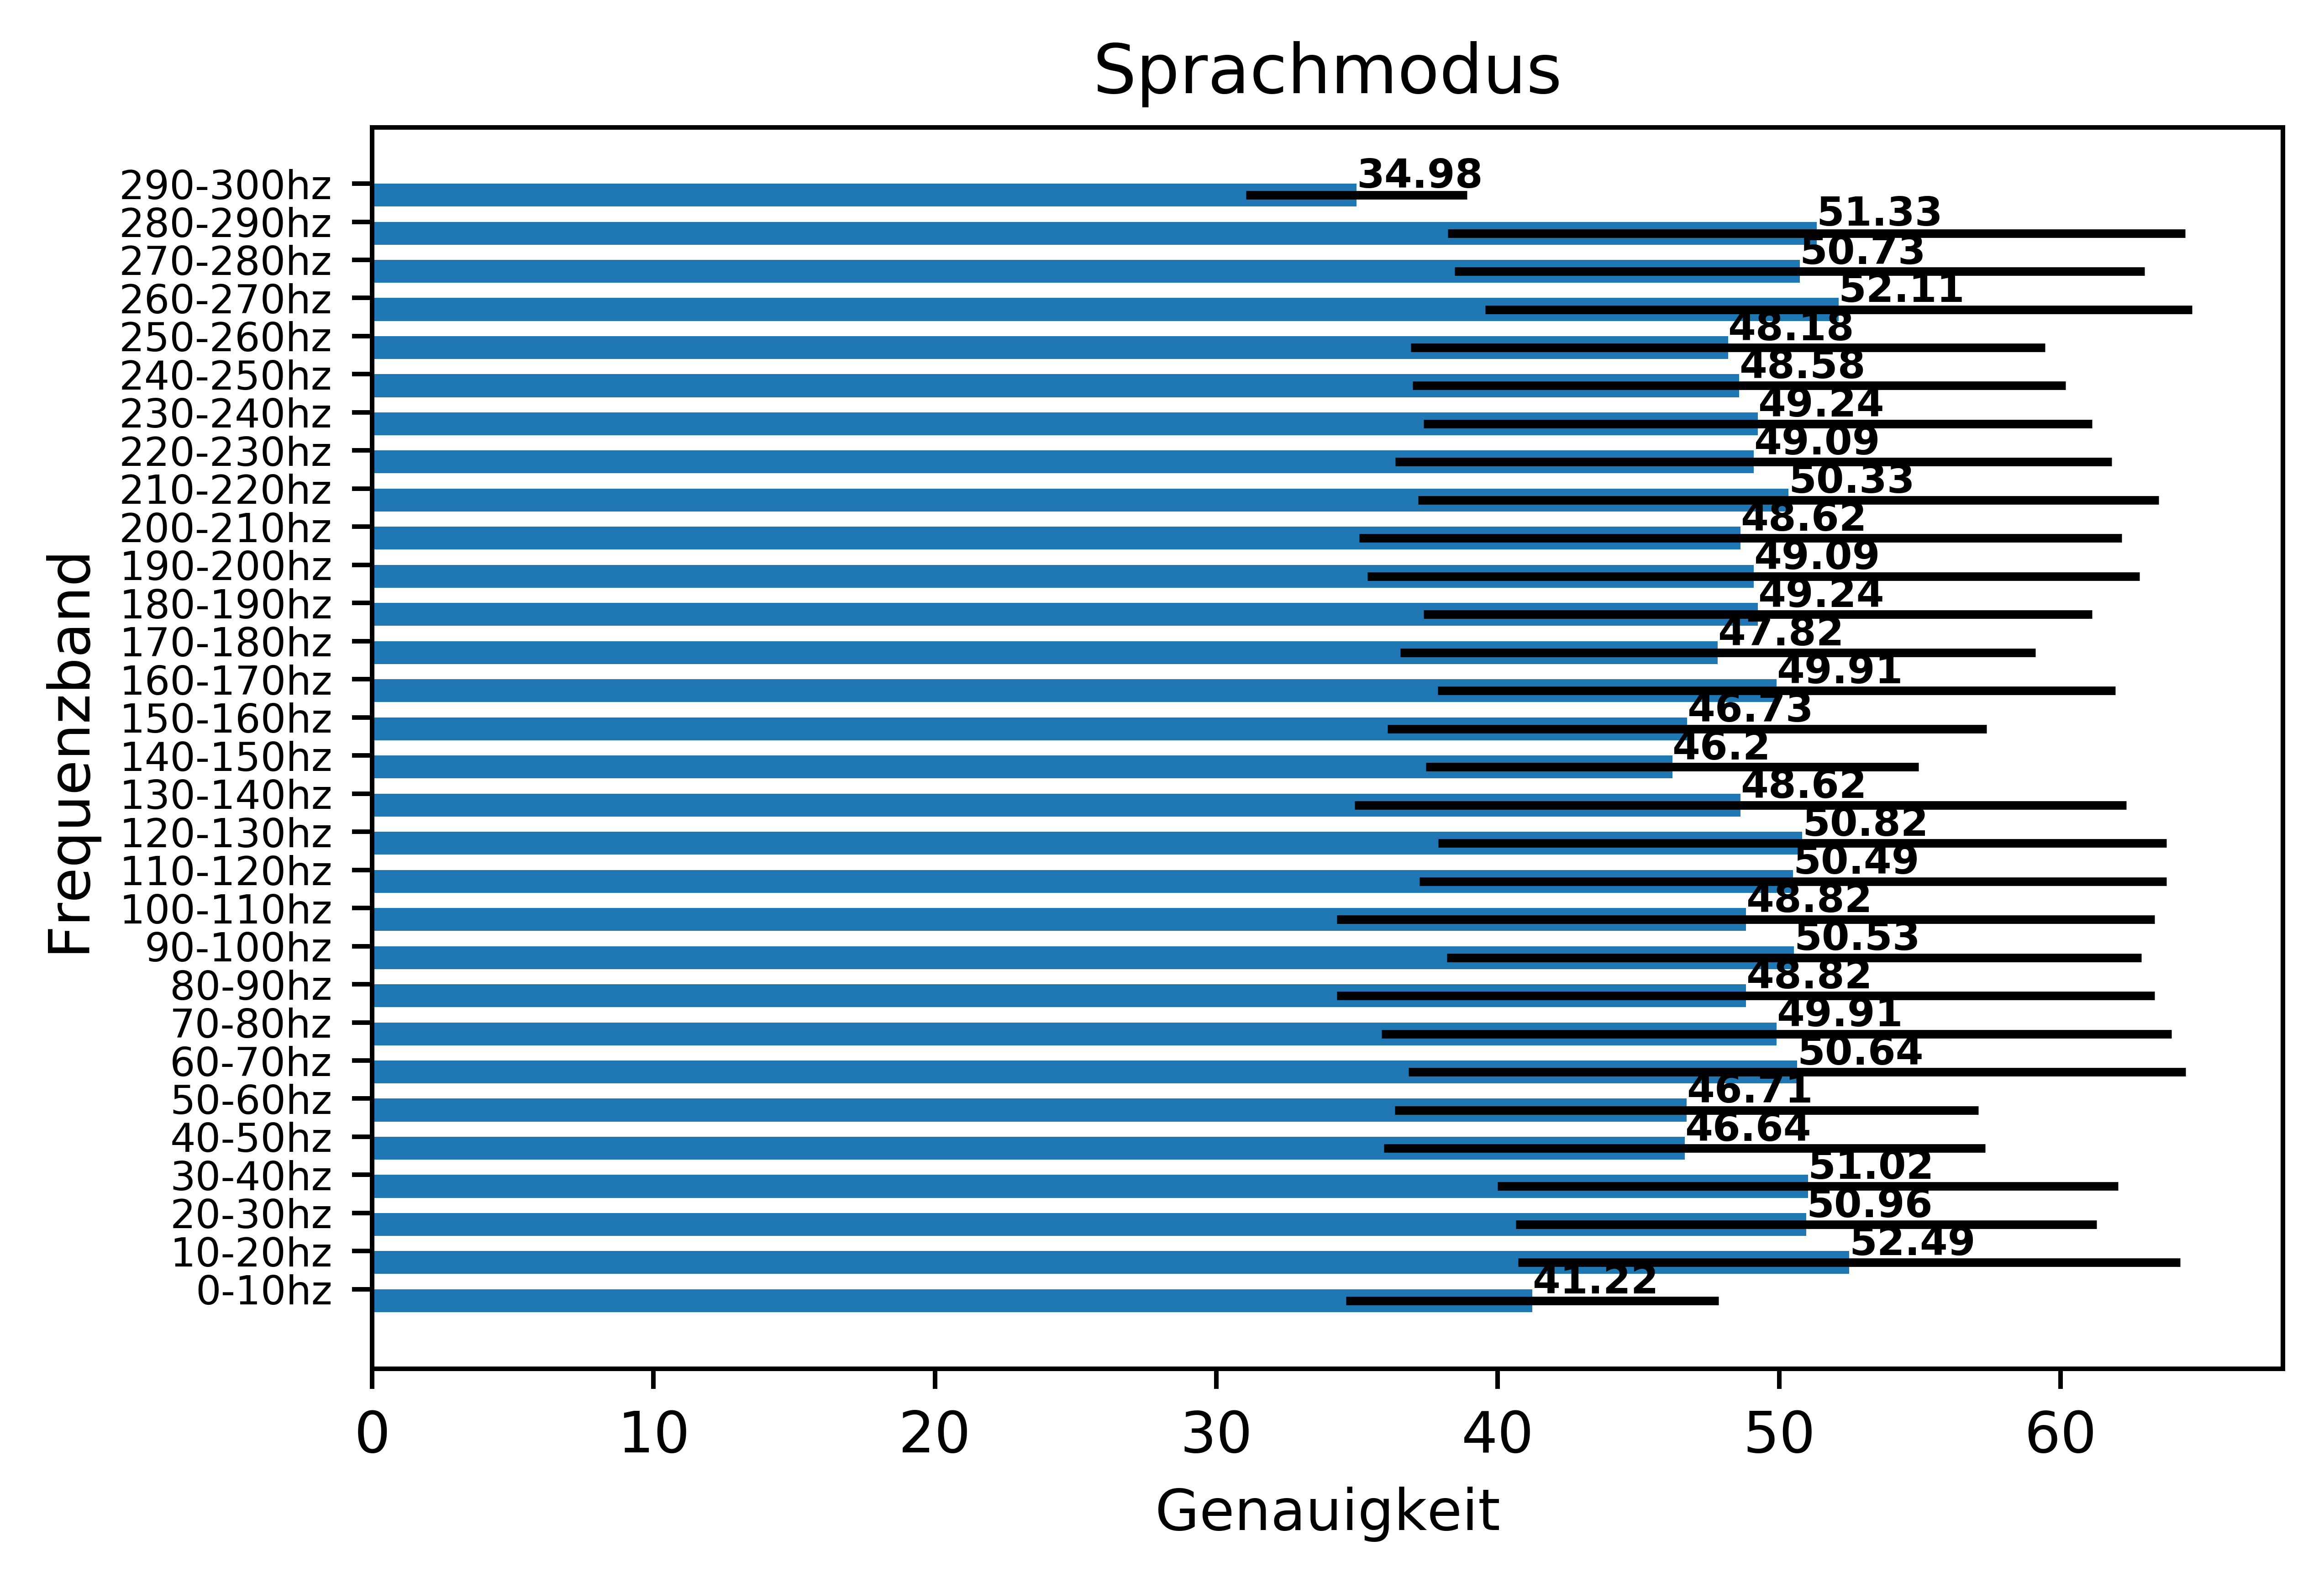
\includegraphics[width=\linewidth]{hzFreqBandResultsSession.png}
  \caption{Die durchschnittliche Genauigkeit, sowie die Standardabweichung der verschiedener Frequenzbänder bei der Erkennung des Sprachmodus. Hier werden die Daten aller Sprecher verwendet die mindestens 2 Sessions besitzen, also die Sprecher 1,2,4,7 und 8. Es handelt sich um Frequenzbänder 0-300Hz in 10Hz Schritten.}
  \label{fig:mode3}
  \end{figure}

\clearpage

\subsection{Cross-User}
Hier wurden die Daten für die Experimente so aufgeteilt das alle Sprecher, welche mehr als eine Session enthalten, genutzt wurden. Es wurde mit allen dieser Sprecher außer einem trainiert und auf dem ausgelassenen wurde getestet. Die Genauigkeiten in den unteren Graphen(\ref{fig:mode4} und \ref{fig:mode5}) sind dabei die durchschnittlichen Werte zwischen den Resultaten von allen Sprechern.

\subsubsection{Ungefiltert}
Hier(\ref{fig:mode4}) wurden die Daten genutzt, ohne sie davor zu filtern. Es ist eine ähnliche Verteilung der Genauigkeit wie in (\ref{fig:mode1}) zu betrachten wobei der LDA, der Randomforest sowie der LinerSVC die höchsten Werte vorweisen. Der LDA-Klassfikator bietet hier wieder, mit 50.04 Prozent, die höchste Genauigkeit. Der KNN-Klassifikator hat die niedrigste Genauigkeit mit 40.24 Prozent.
Bei den Confusion-Matrix Analysen (\ref{fig:cnfsunfiltered}) wurden ein LDA verwendet.

\begin{figure}[H]
  \centering
  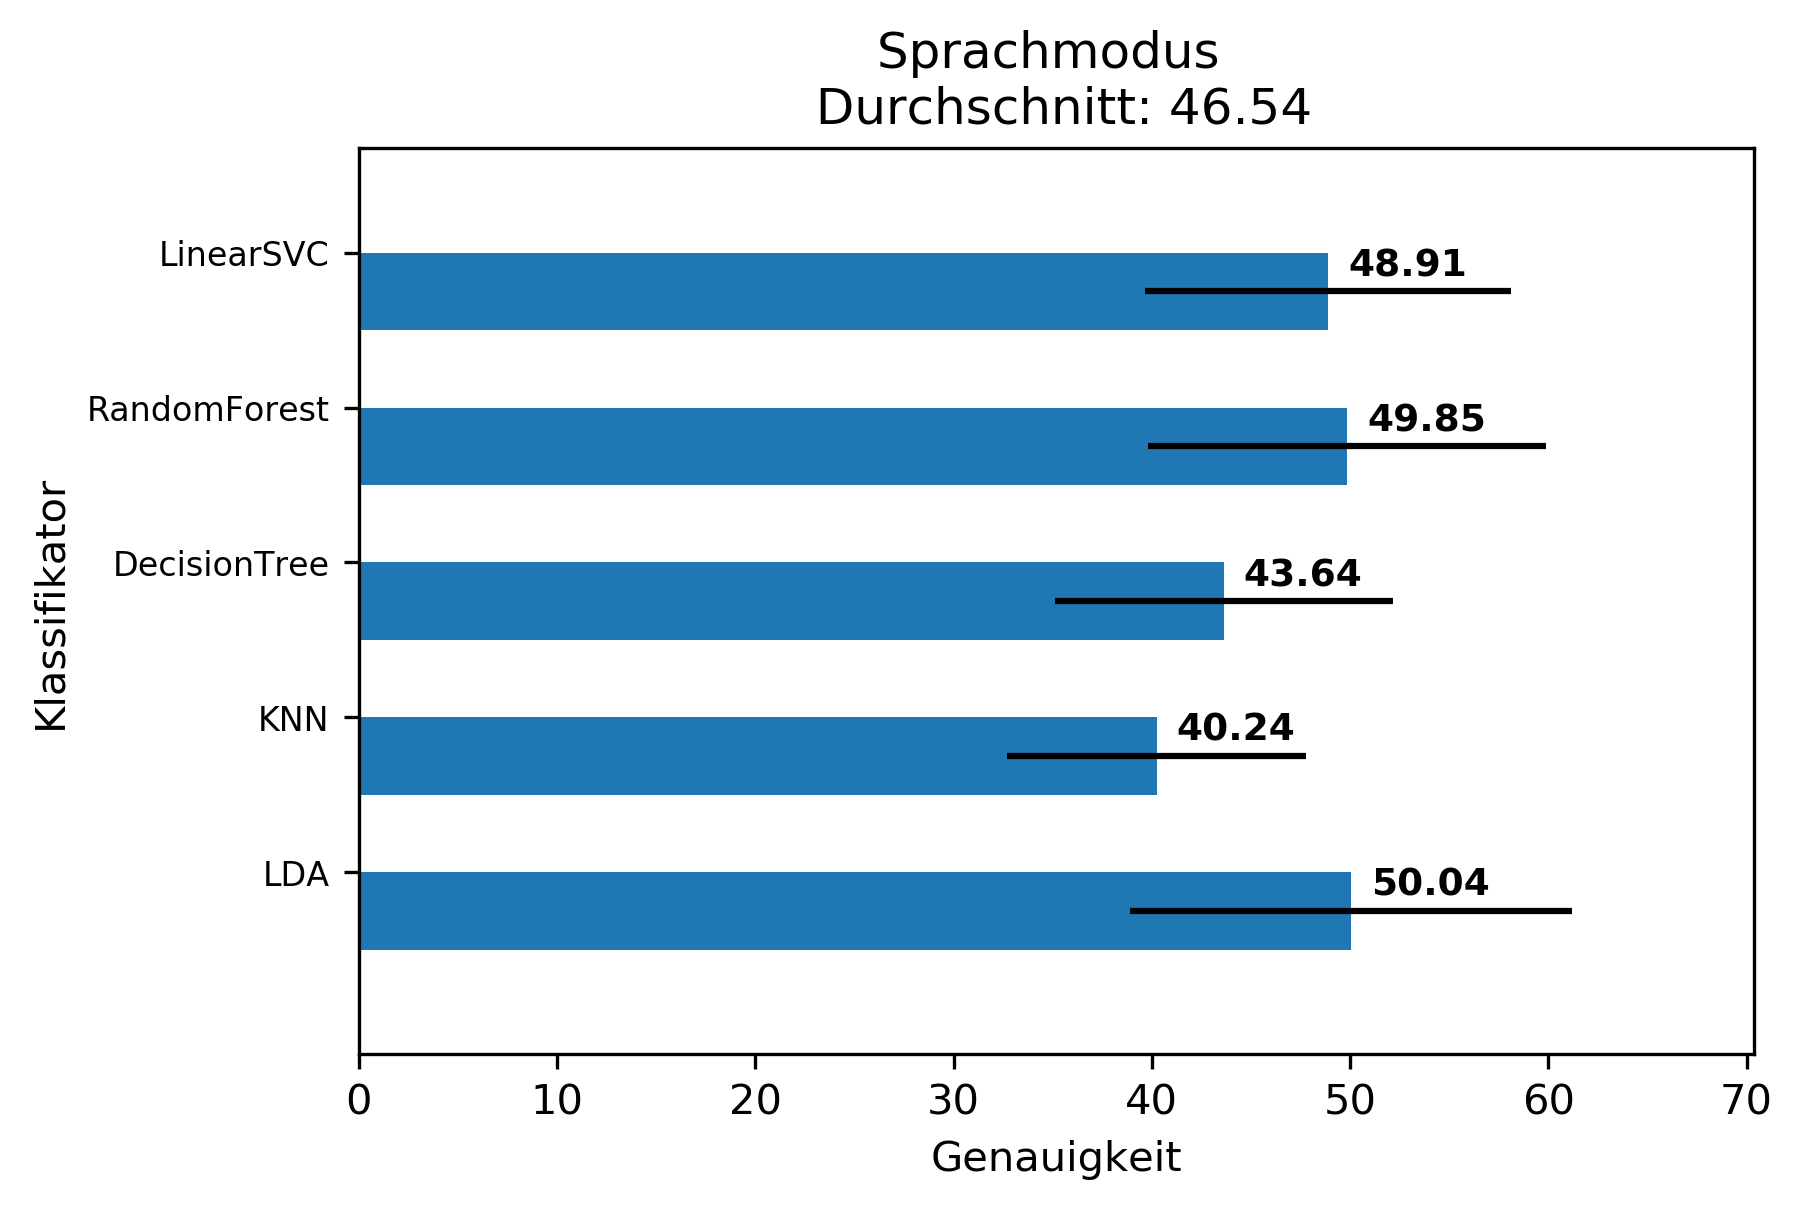
\includegraphics[width=100mm ,scale=0.6]{modeResultsUserUnfiltered.png}
  \caption{Die durchschnittliche Genauigkeit, sowie die Standardabweichung der verschiedener Klassifikatoren bei der Erkennung des Sprachmodus.Hier werden die Daten aller Sprecher verwendet die mindestens 2 Sessions besitzen, also die Sprecher 1,2,4,7 und 8}
  \label{fig:mode4}
\end{figure}

\clearpage

In \ref{fig:cnf10} sieht man das bei Sprecher 1, bei audible und whisper zu 99 Prozent whisper vorhergesagt.

In \ref{fig:cnf11} sieht man das bei Sprecher 2, größtenteils audible vorhergesagt wird. Es wird zu 83–86 Prozent audible vorhergesagt und zu 13–14 Prozent whisper.

Sprecher 3 (\ref{fig:cnf12}) ist der erste Sprecher, bei der eine Verteilung der Vorhersagen zu sehen ist, in der nicht eine der Möglichkeiten immer wieder ausgewählt wurde. Stadtessen sieht man eine 92 prozentige Genauigkeit für silent und eine 84 prozentige Genauigkeit für whisper. Lediglich audible hat man 10 Prozent eine niedrige Genauigkeit.

Bei Sprecher 4 (\ref{fig:cnf13}) ist eine Verteilung der Vorhersagen zu sehen, die etwas besser als die von den ersten beiden Sprechern ist. Man kann eine 81 prozentige Genauigkeit für whisper. Für die restlichen Zustände lässt sich eine sehr zufällige Verteilung erkennen. Audible wird entweder als audible oder als whisper erkannt und silent wird größtenteils, nämlich zu 49 Prozent als whisper erkannt.

Bei Sprecher 5 (\ref{fig:cnf14}) ist eine richtige Vorhersage von audible zu 82 Prozent und silent zu 94 Prozent zu sehen. Lediglich der whisper Sprachmodus hat bei diesem Sprecher mit 32 Prozent keine gute Genauigkeit.

Für Sprecher 6 (\ref{fig:cnf15}) ist eine richtige Vorhersage von silent zu 98 Prozent zu sehen. Die zwei anderen Sprachmodi werden nicht gut erkannt. Whisper wird zu 74 Prozent als silent eingestuft und audible zu 58 Prozent als whisper.

Bei Sprecher 7 (\ref{fig:cnf16}) ist eine richtige Vorhersage von silent in 99 Prozent der Fälle zu beobachten. Die zwei anderen Sprachmodi werden nicht gut erkannt. Whisper wird zu 63 Prozent mit silent verwechselt und zu 37 Prozent als audible. Audible zu 55 Prozent als silent und 45 Prozent als audible. Der whisper Sprachmodus wird bei diesem Sprecher überhaupt nicht vorhergesagt.

Für Sprecher 8 (\ref{fig:cnf17}) wird zum Großteil nur silent vorhergesagt egal um welchen Sprachmodus es sich handelt.

Es fällt auf, dass sich bei dem Sprecher 3 sowie bei Sprecher 5–8 eine über 90 Prozent Genauigkeit für den silent Sprachmodus erkennen lässt, wobei Sprecher 8 in allen Bereichen silent klassifiziert hat. Zudem haben Sprecher 1,3 und 4 eine über 90 Prozent Genauigkeit für den whisper Sprachmodus.

\begin{figure}[H]
\centering     %%% not \center
\subfigure[Sprecher 1]{\label{fig:cnf10}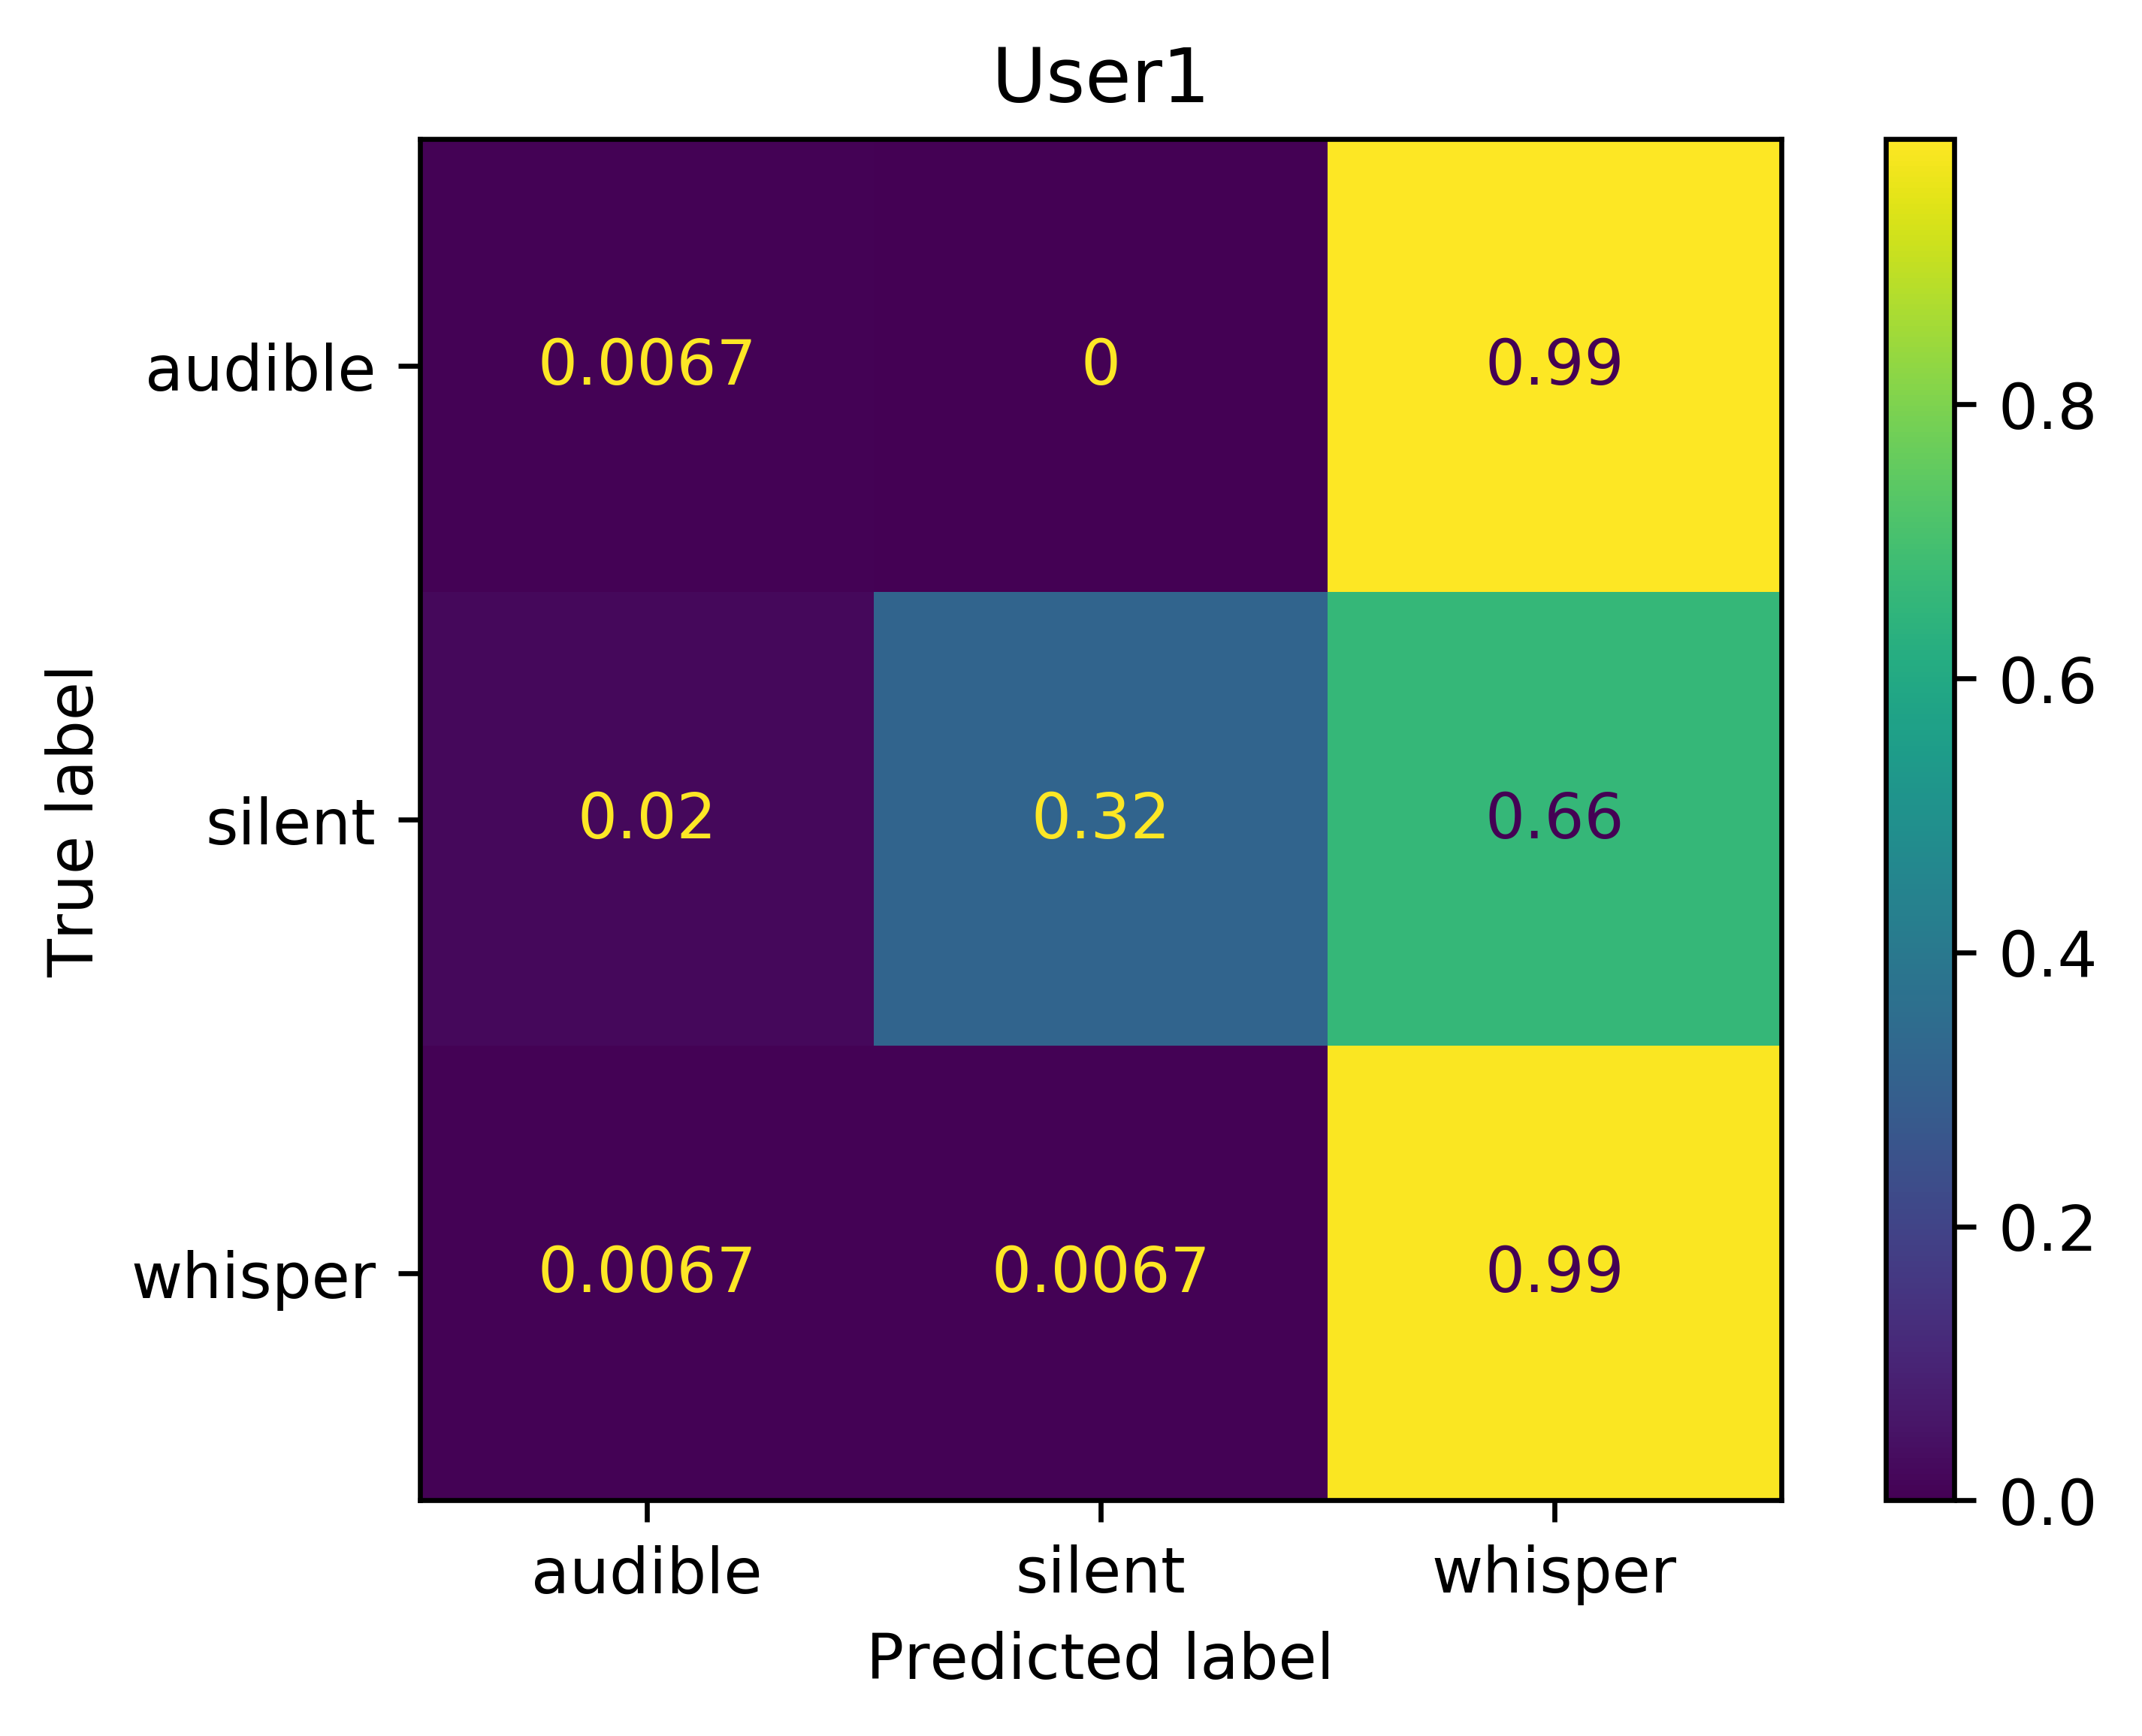
\includegraphics[width=63mm]{modeCrossUserUnf/User1_unf.png}}
\subfigure[Sprecher 2]{\label{fig:cnf11}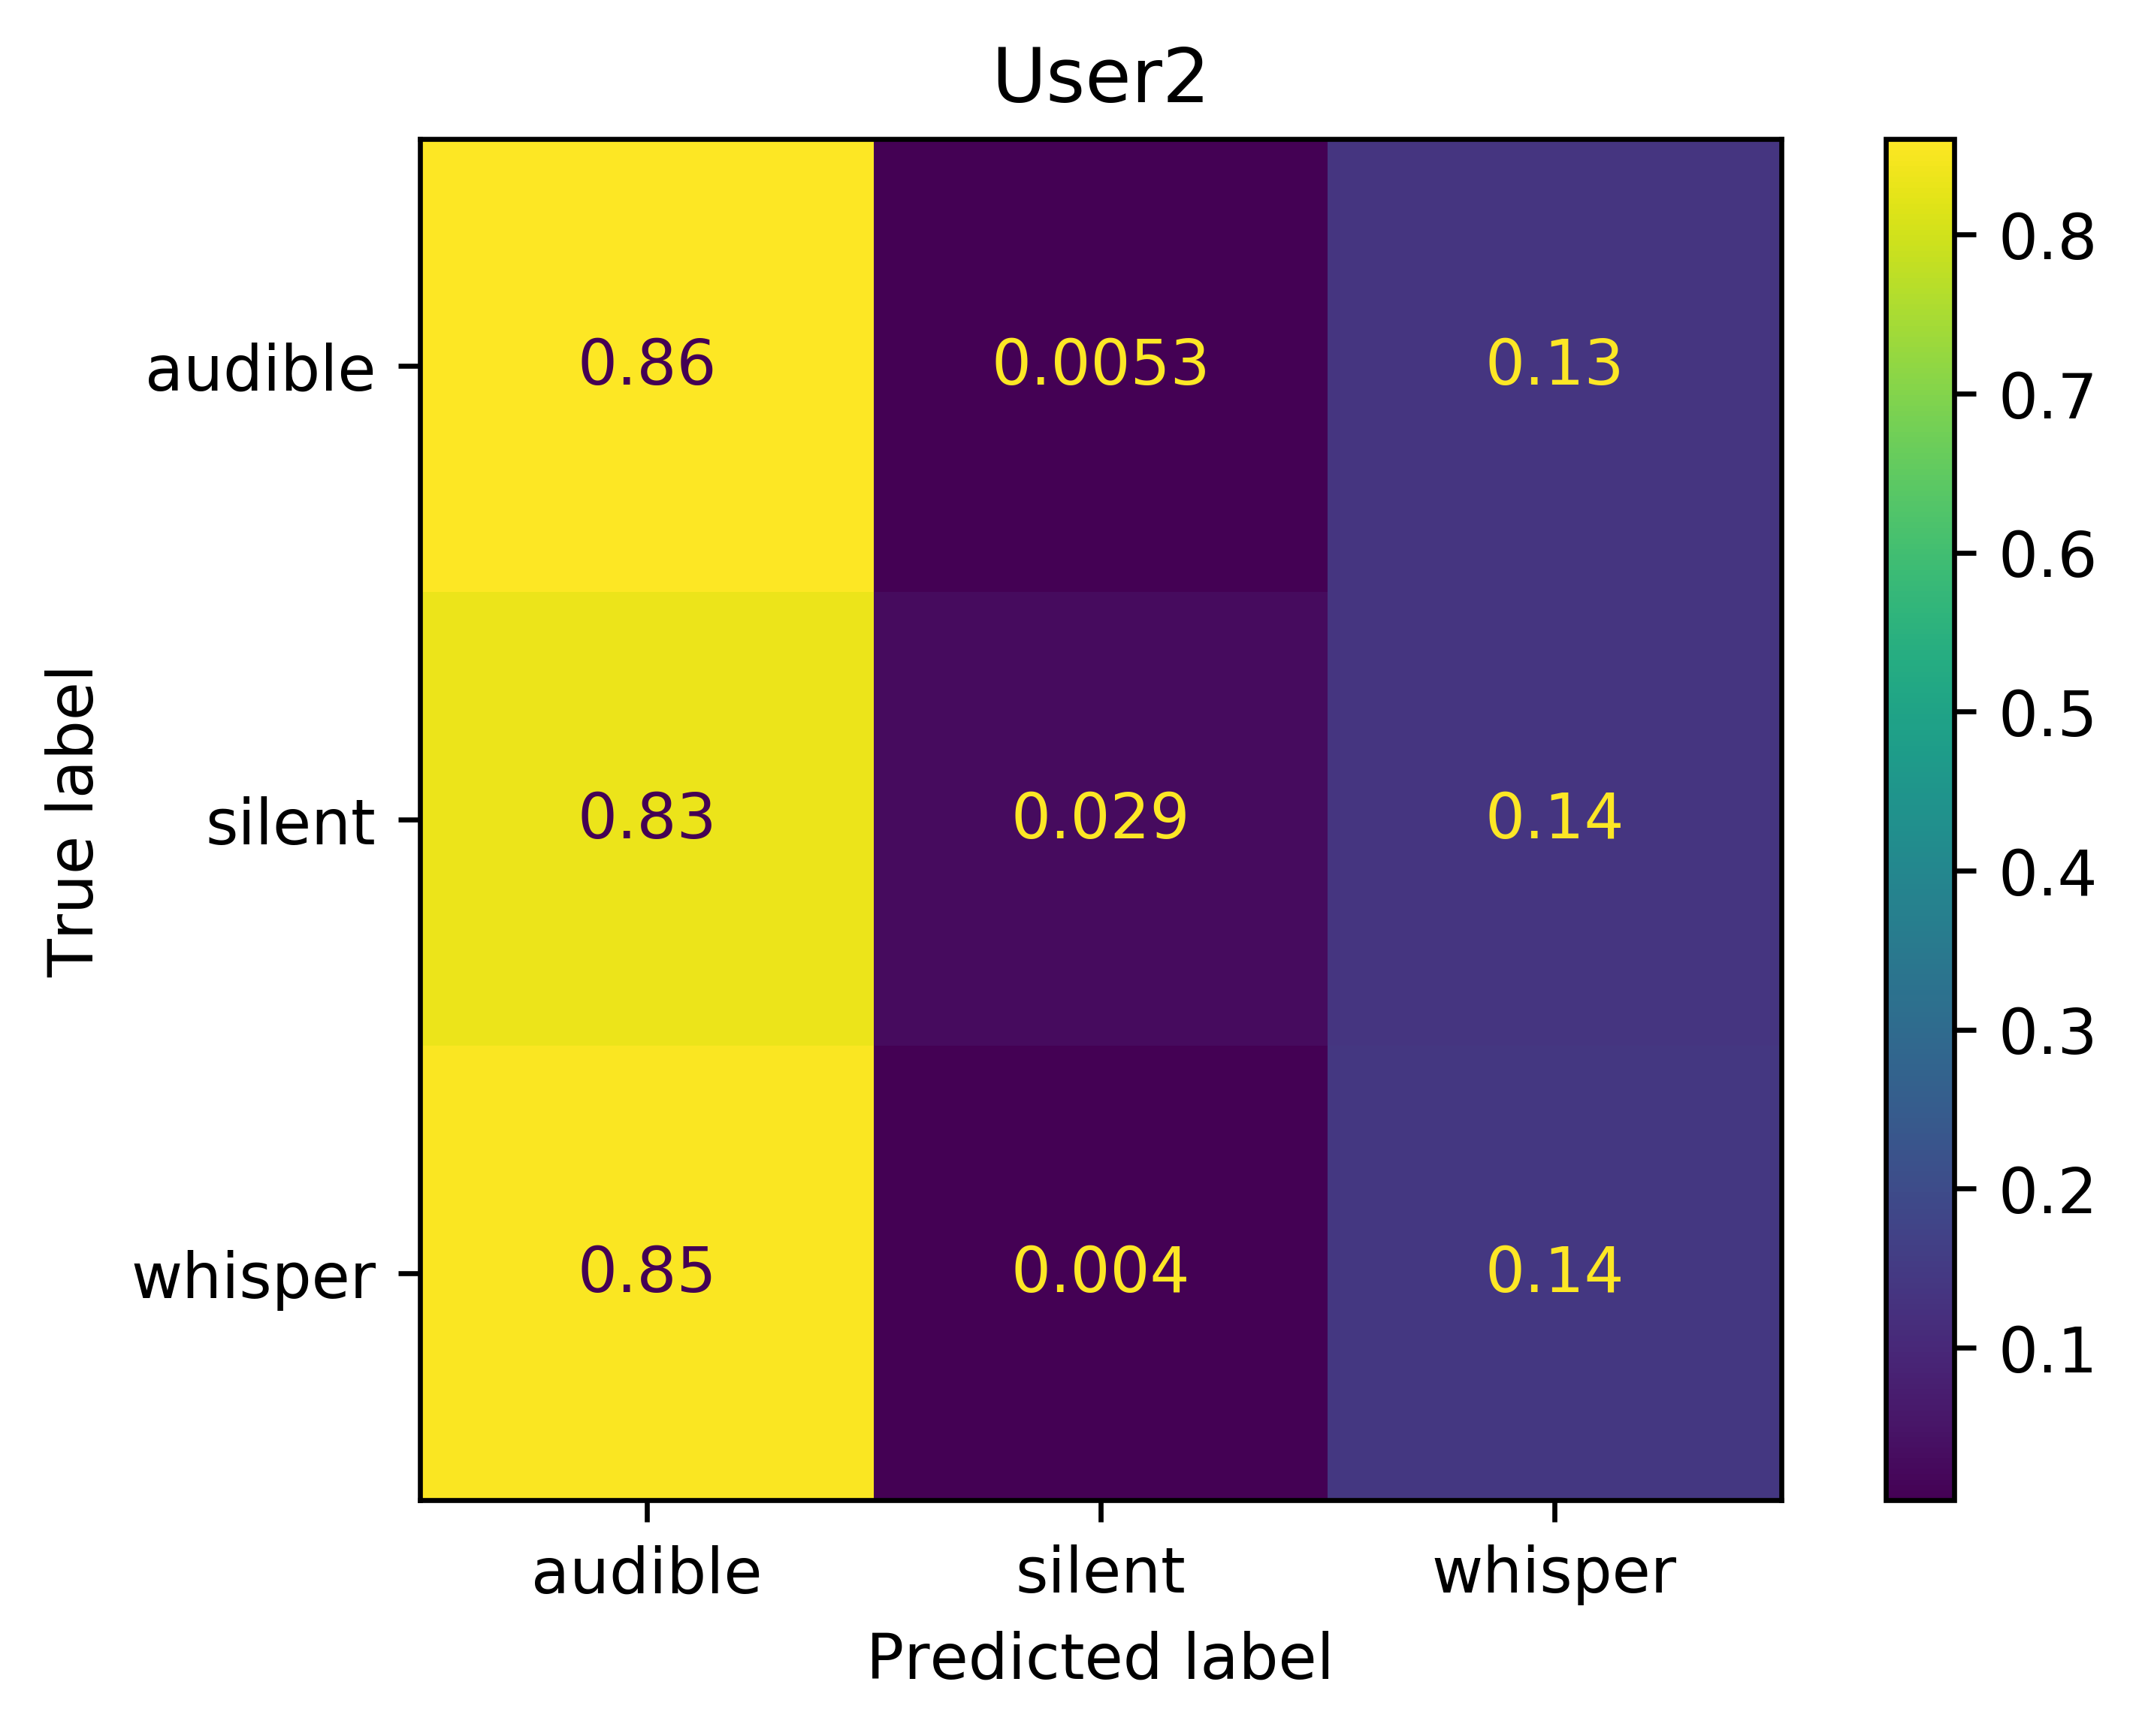
\includegraphics[width=63mm]{modeCrossUserUnf/User2_unf.png}}
\subfigure[Sprecher 3]{\label{fig:cnf12}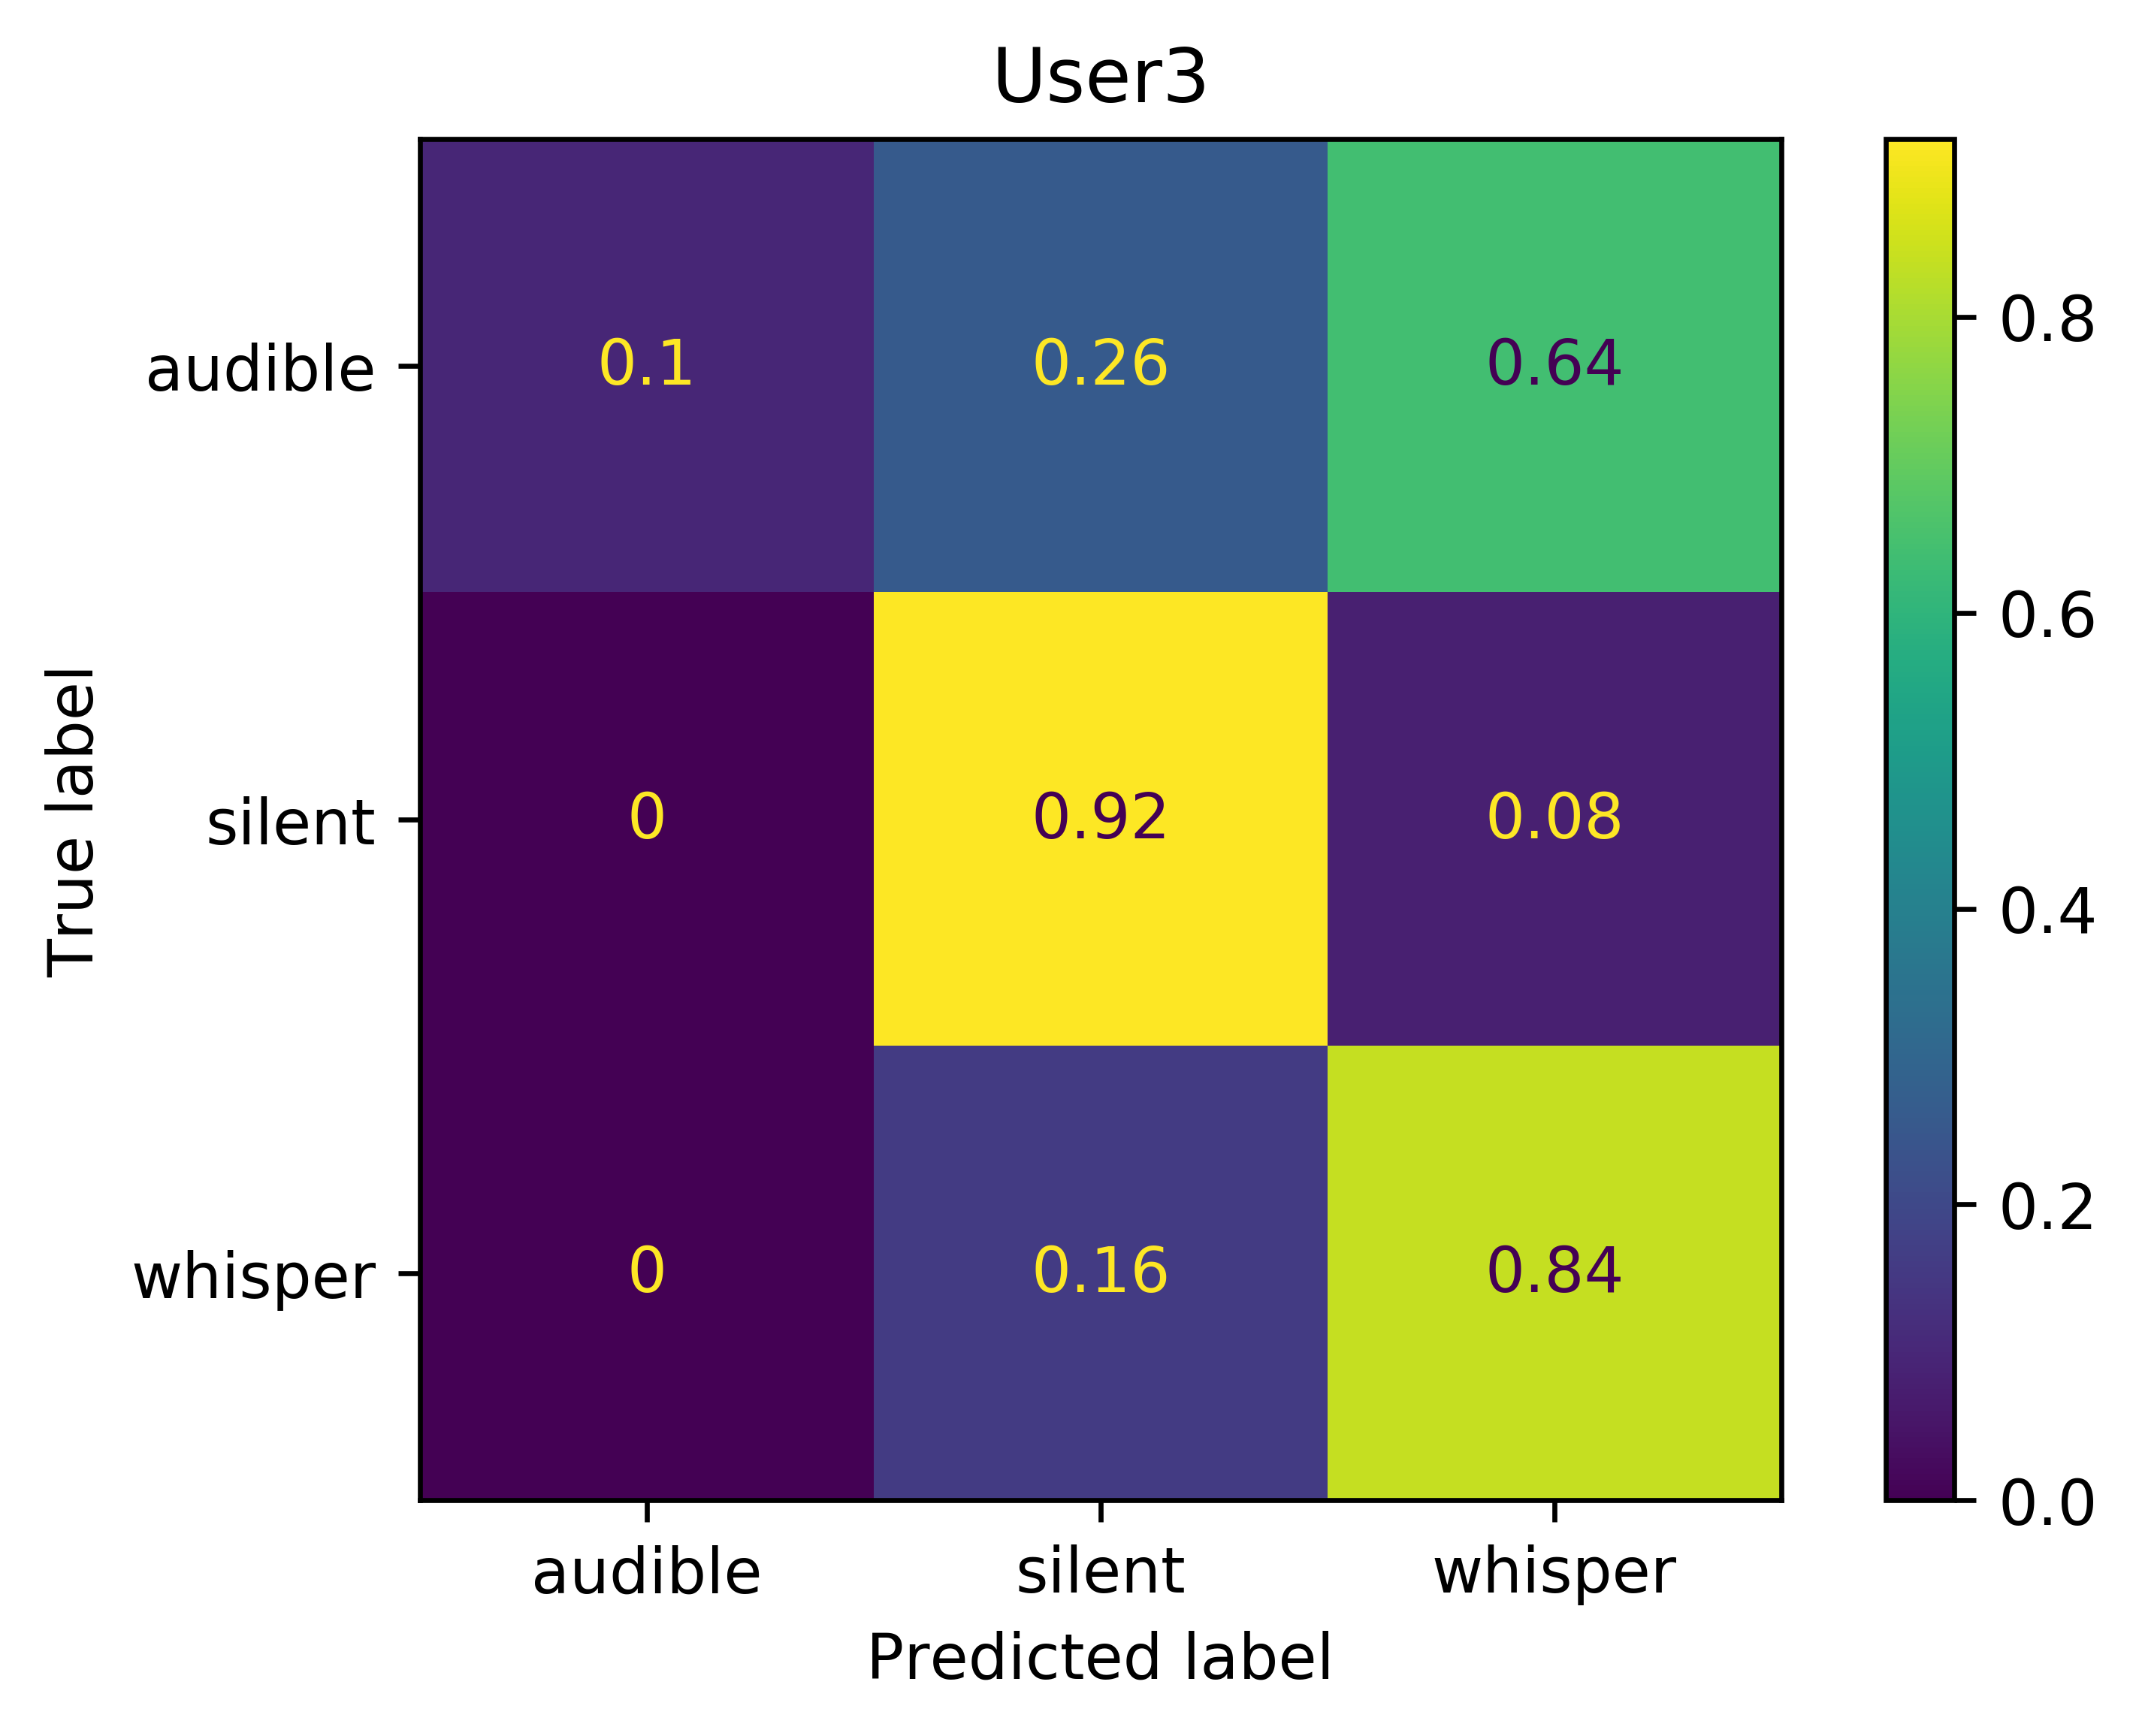
\includegraphics[width=63mm]{modeCrossUserUnf/User3_unf.png}}
\subfigure[Sprecher 4]{\label{fig:cnf13}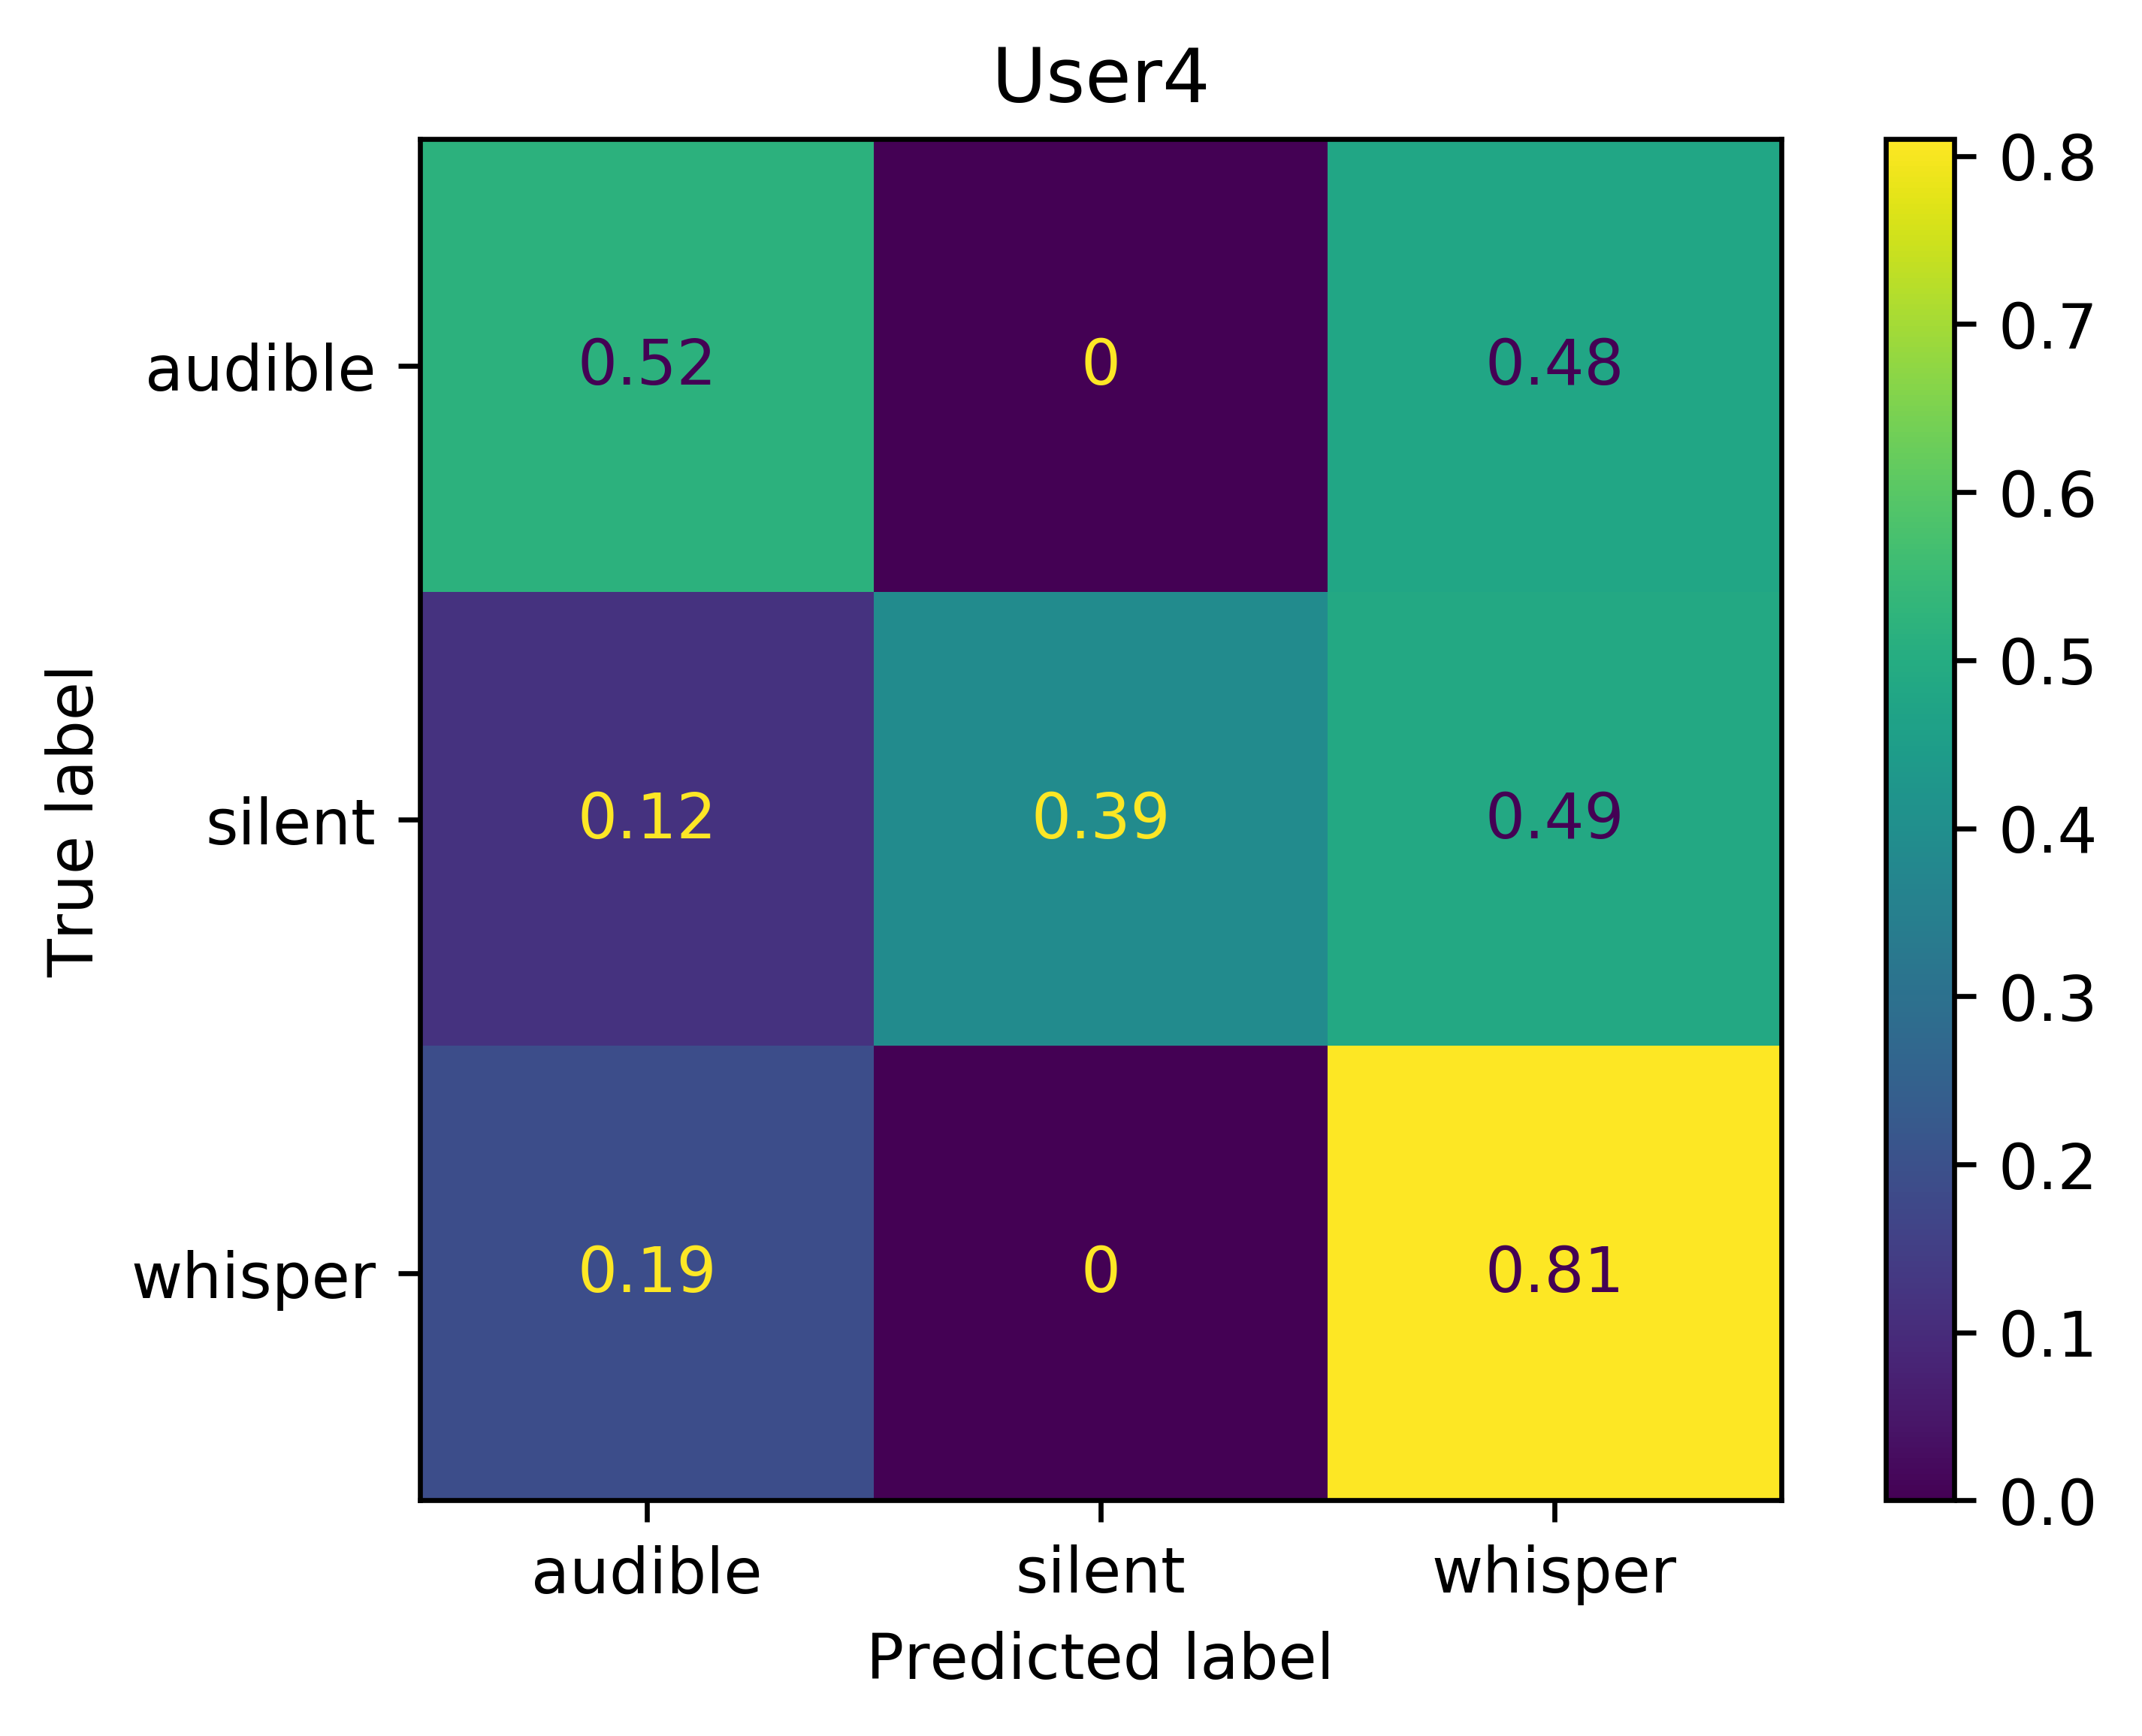
\includegraphics[width=63mm]{modeCrossUserUnf/User4_unf.png}}
\subfigure[Sprecher 5]{\label{fig:cnf14}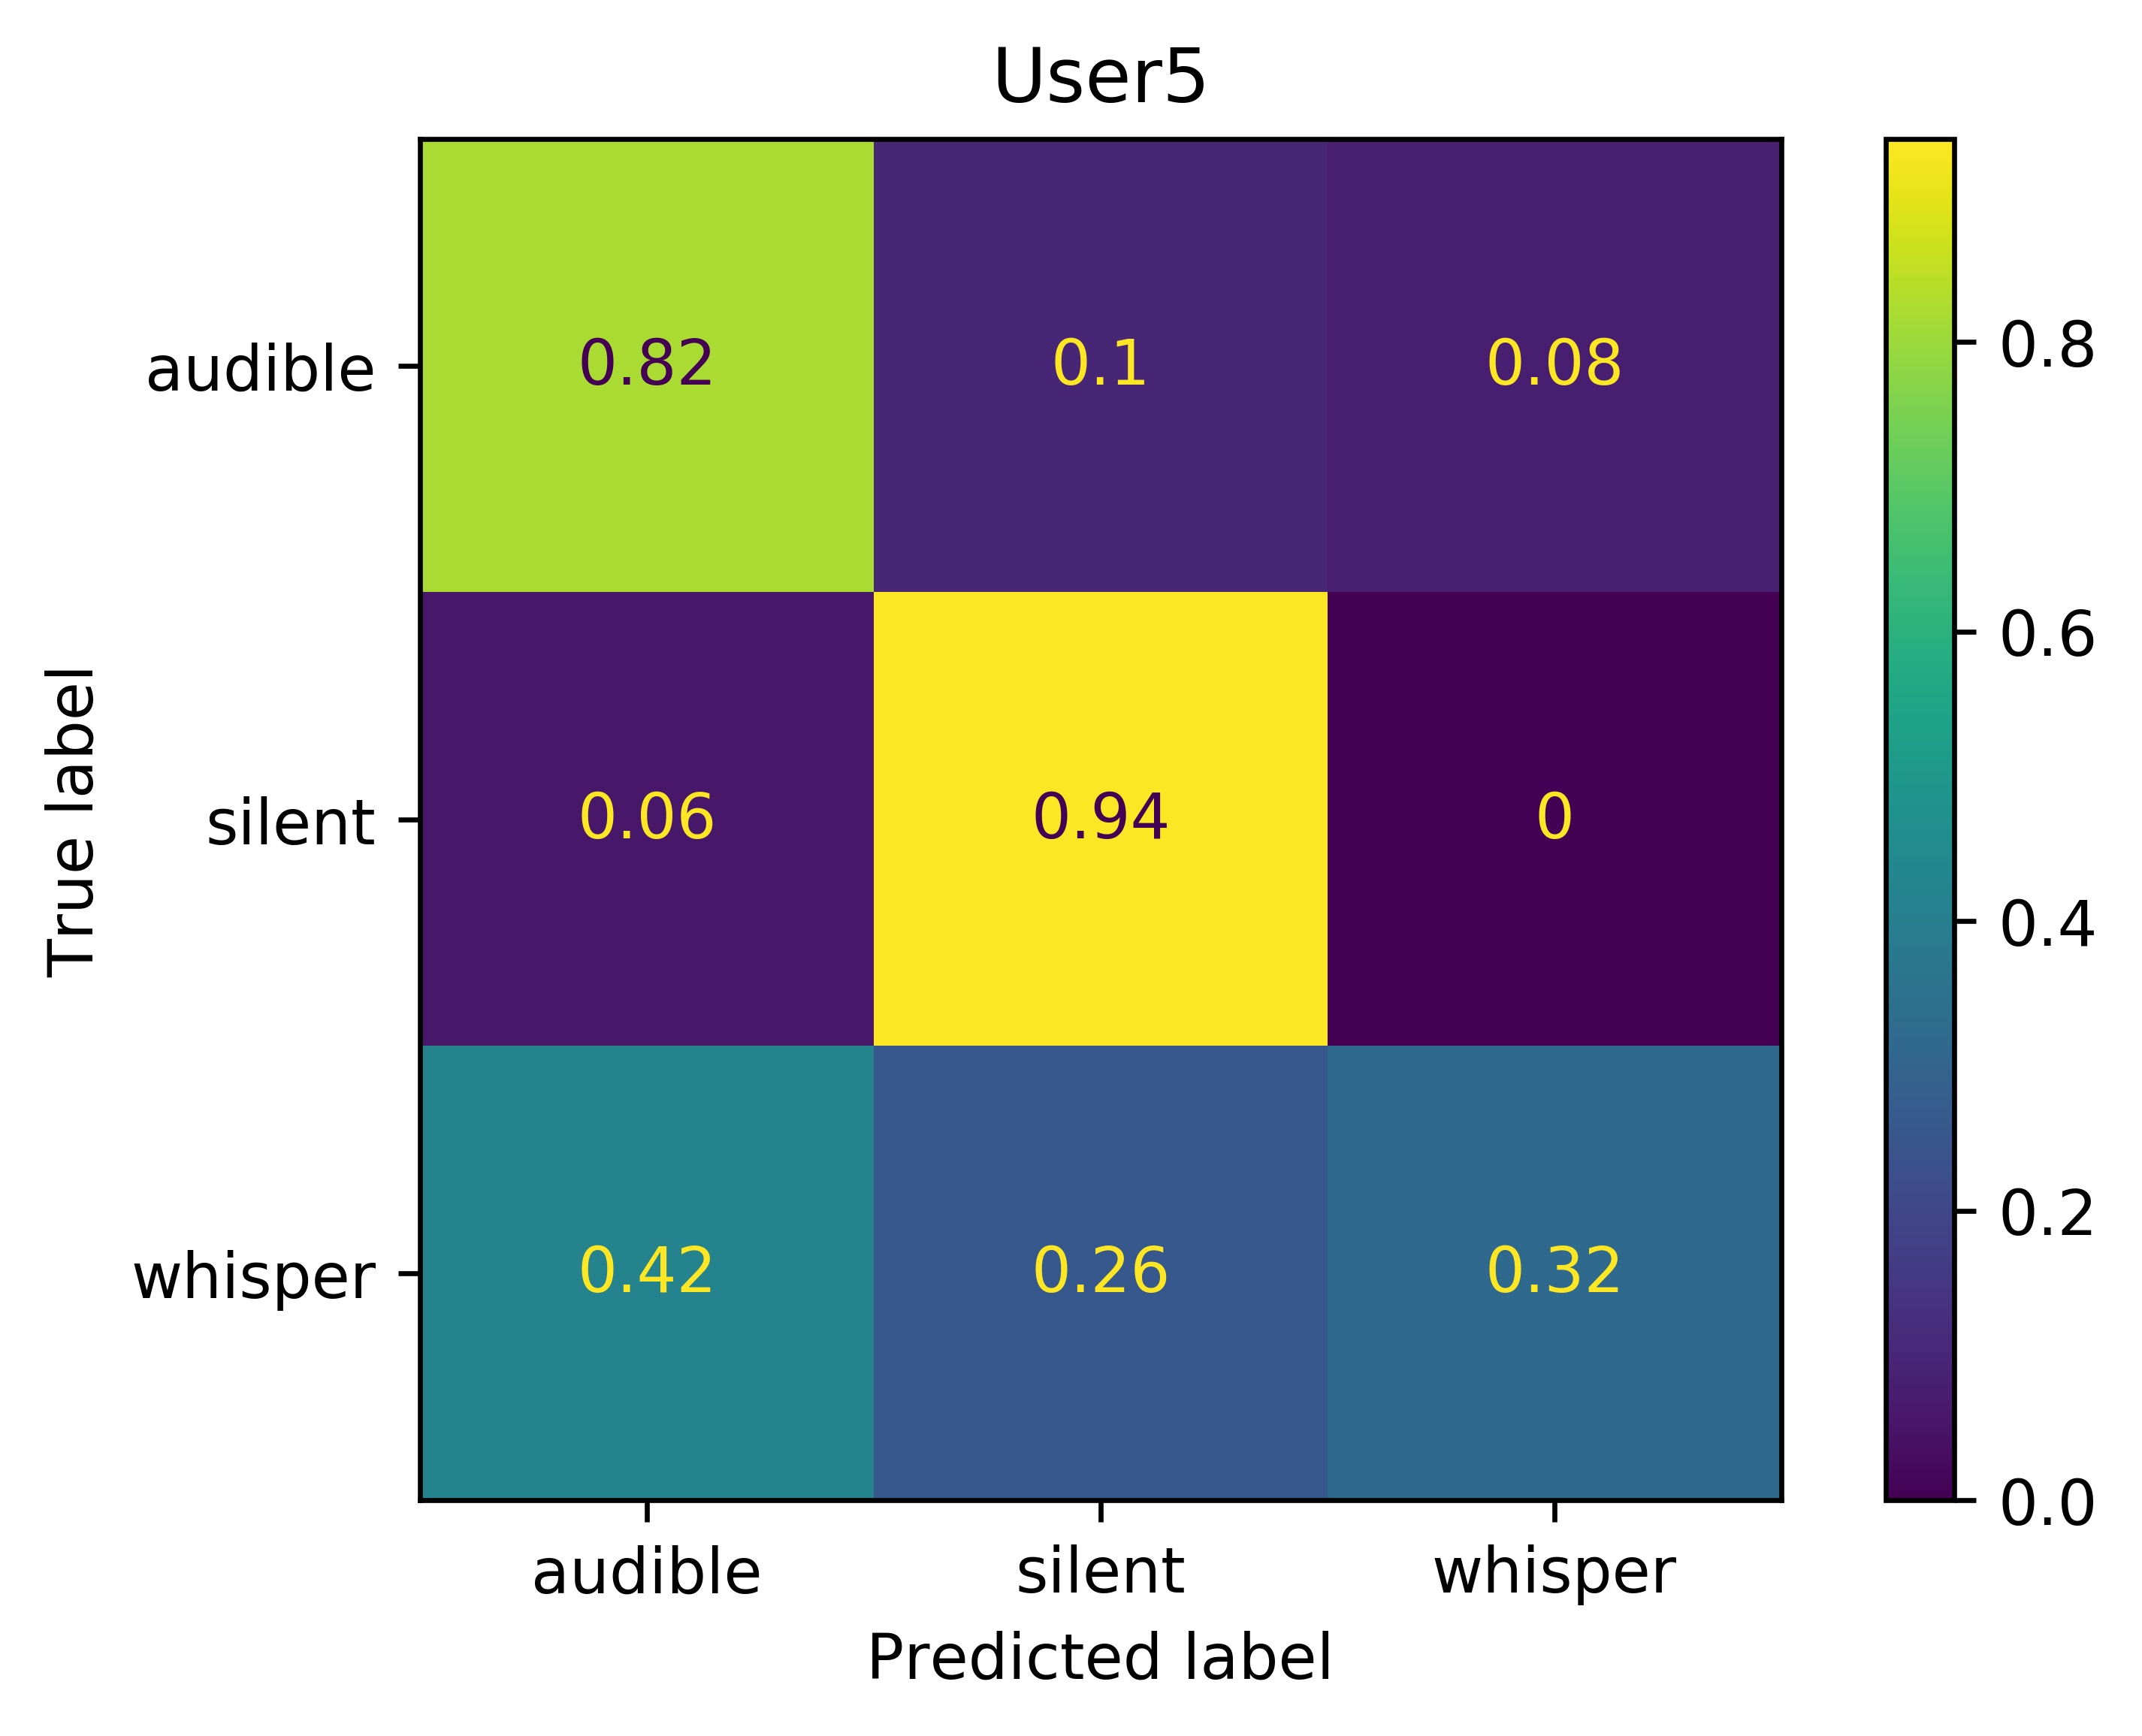
\includegraphics[width=63mm]{modeCrossUserUnf/User5_unf.png}}
\subfigure[Sprecher 6]{\label{fig:cnf15}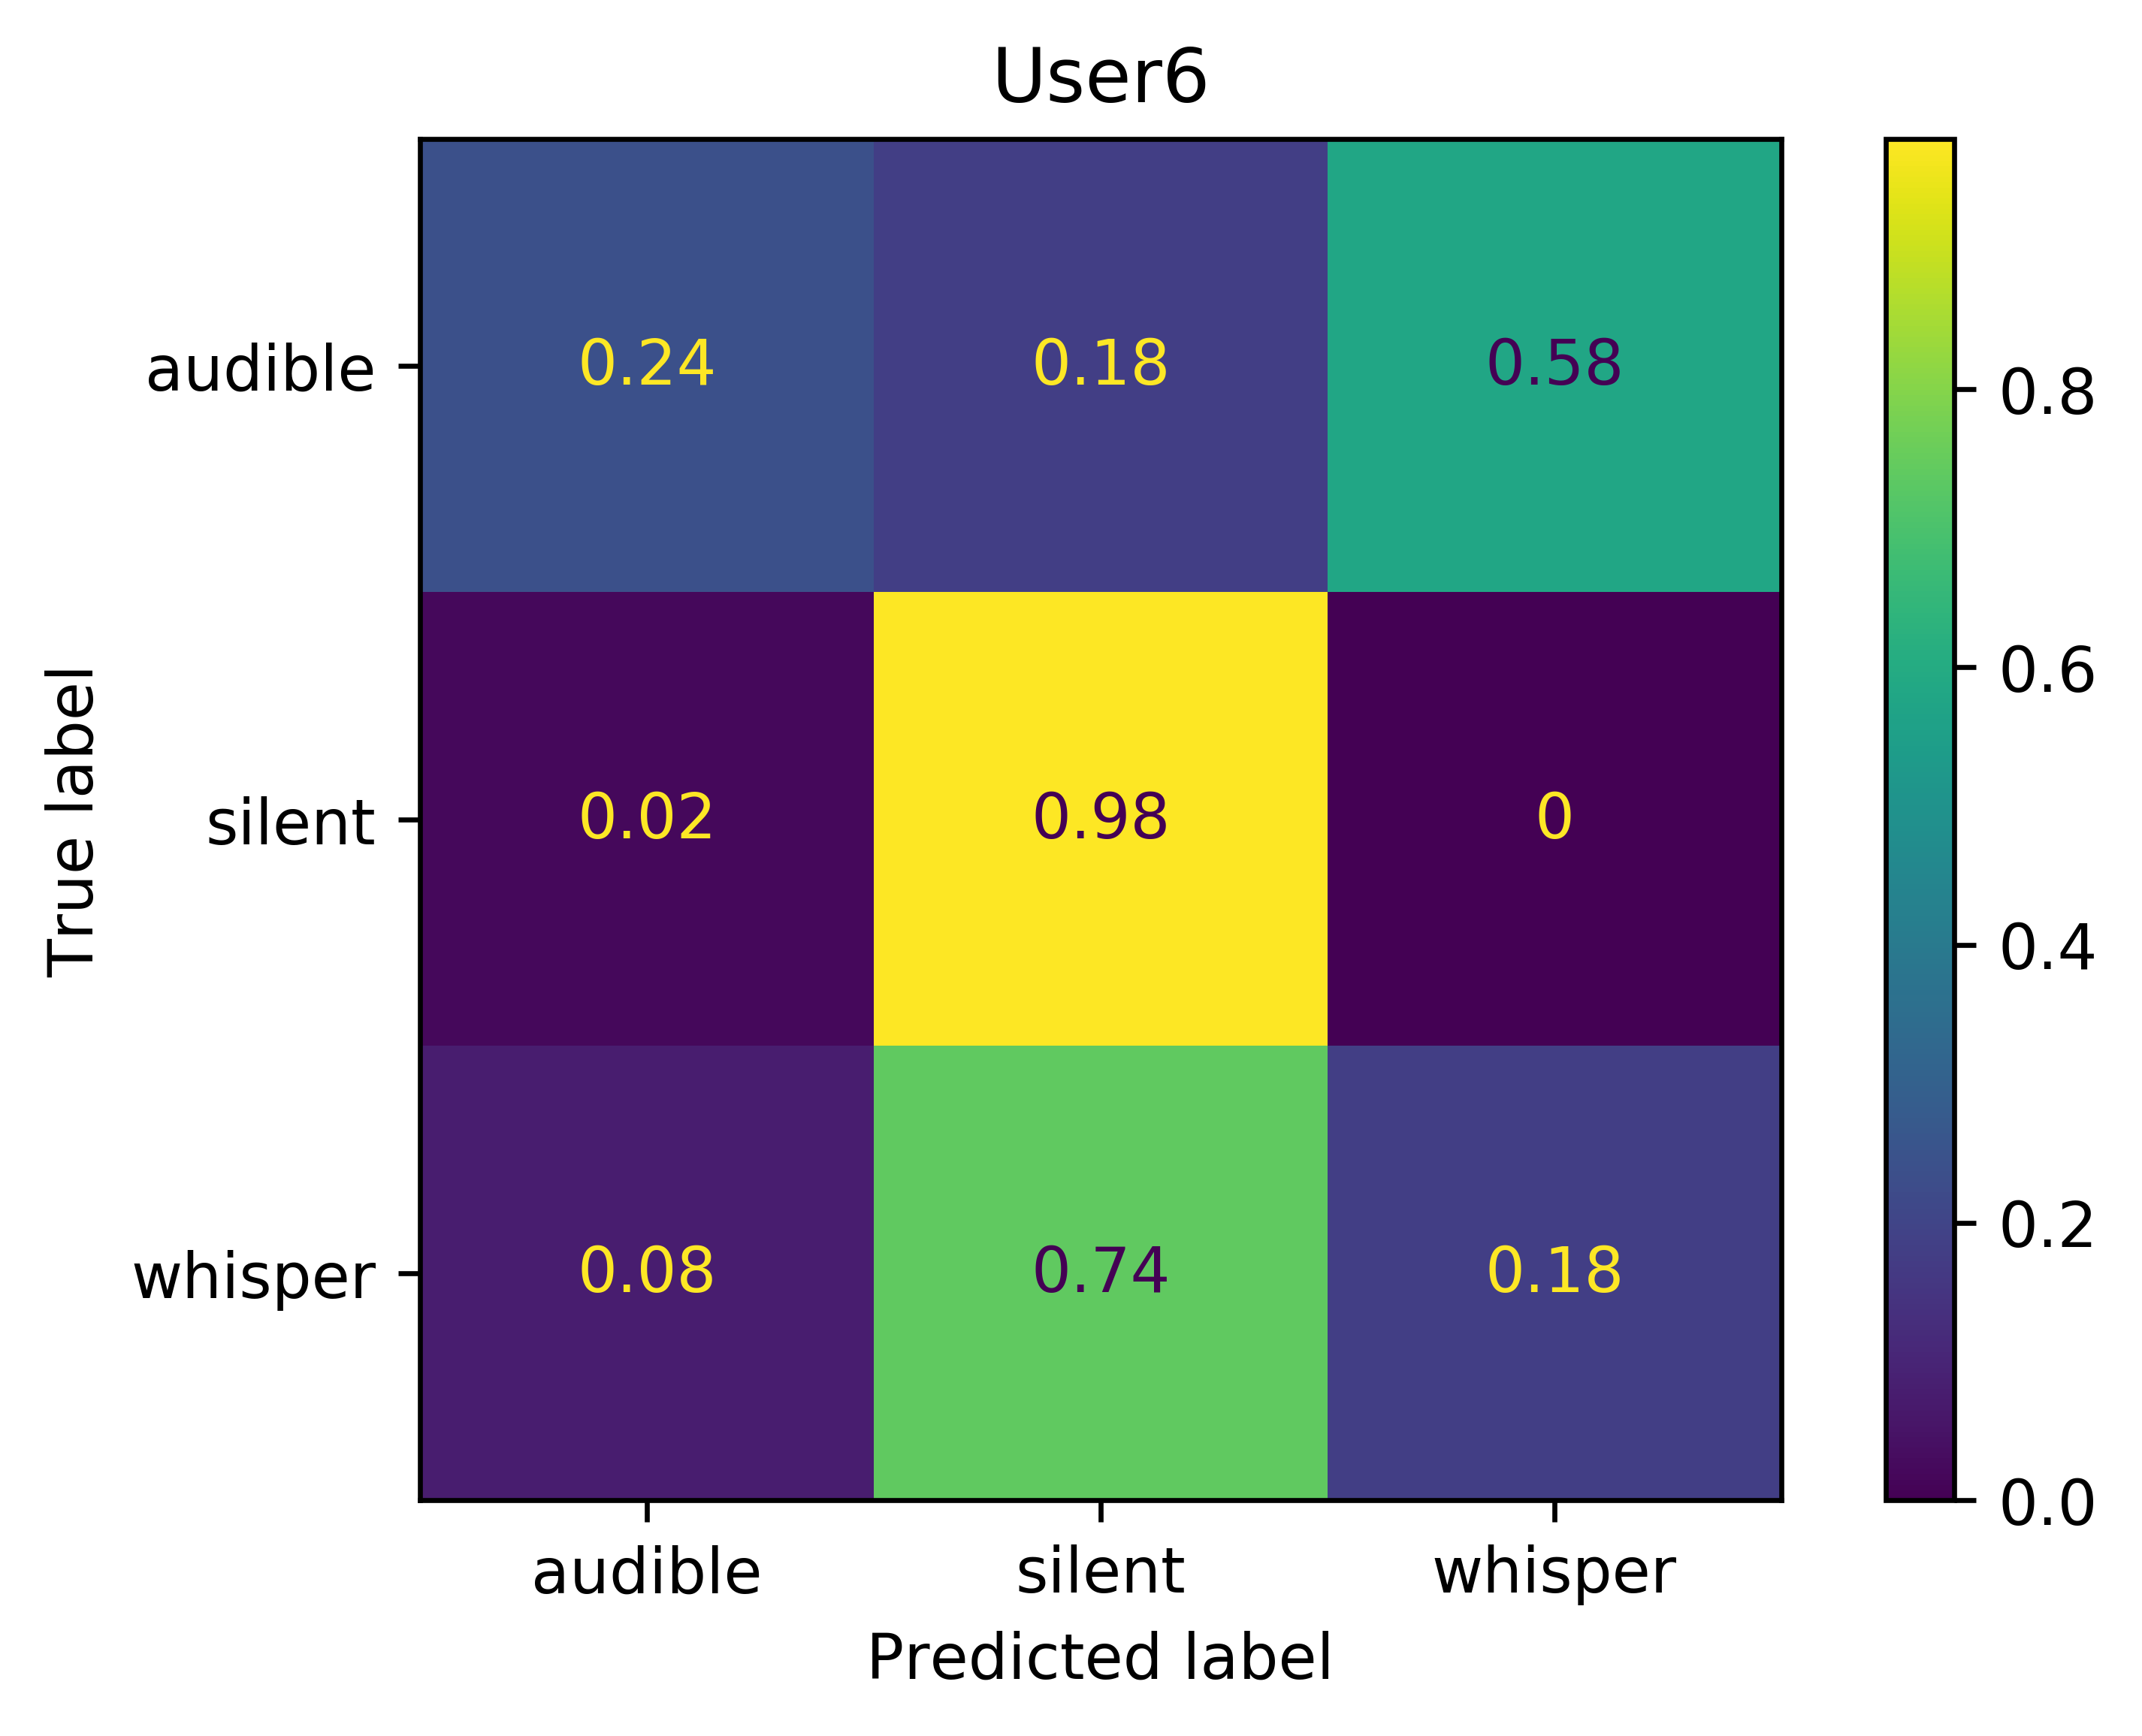
\includegraphics[width=63mm]{modeCrossUserUnf/User6_unf.png}}
\subfigure[Sprecher 7]{\label{fig:cnf16}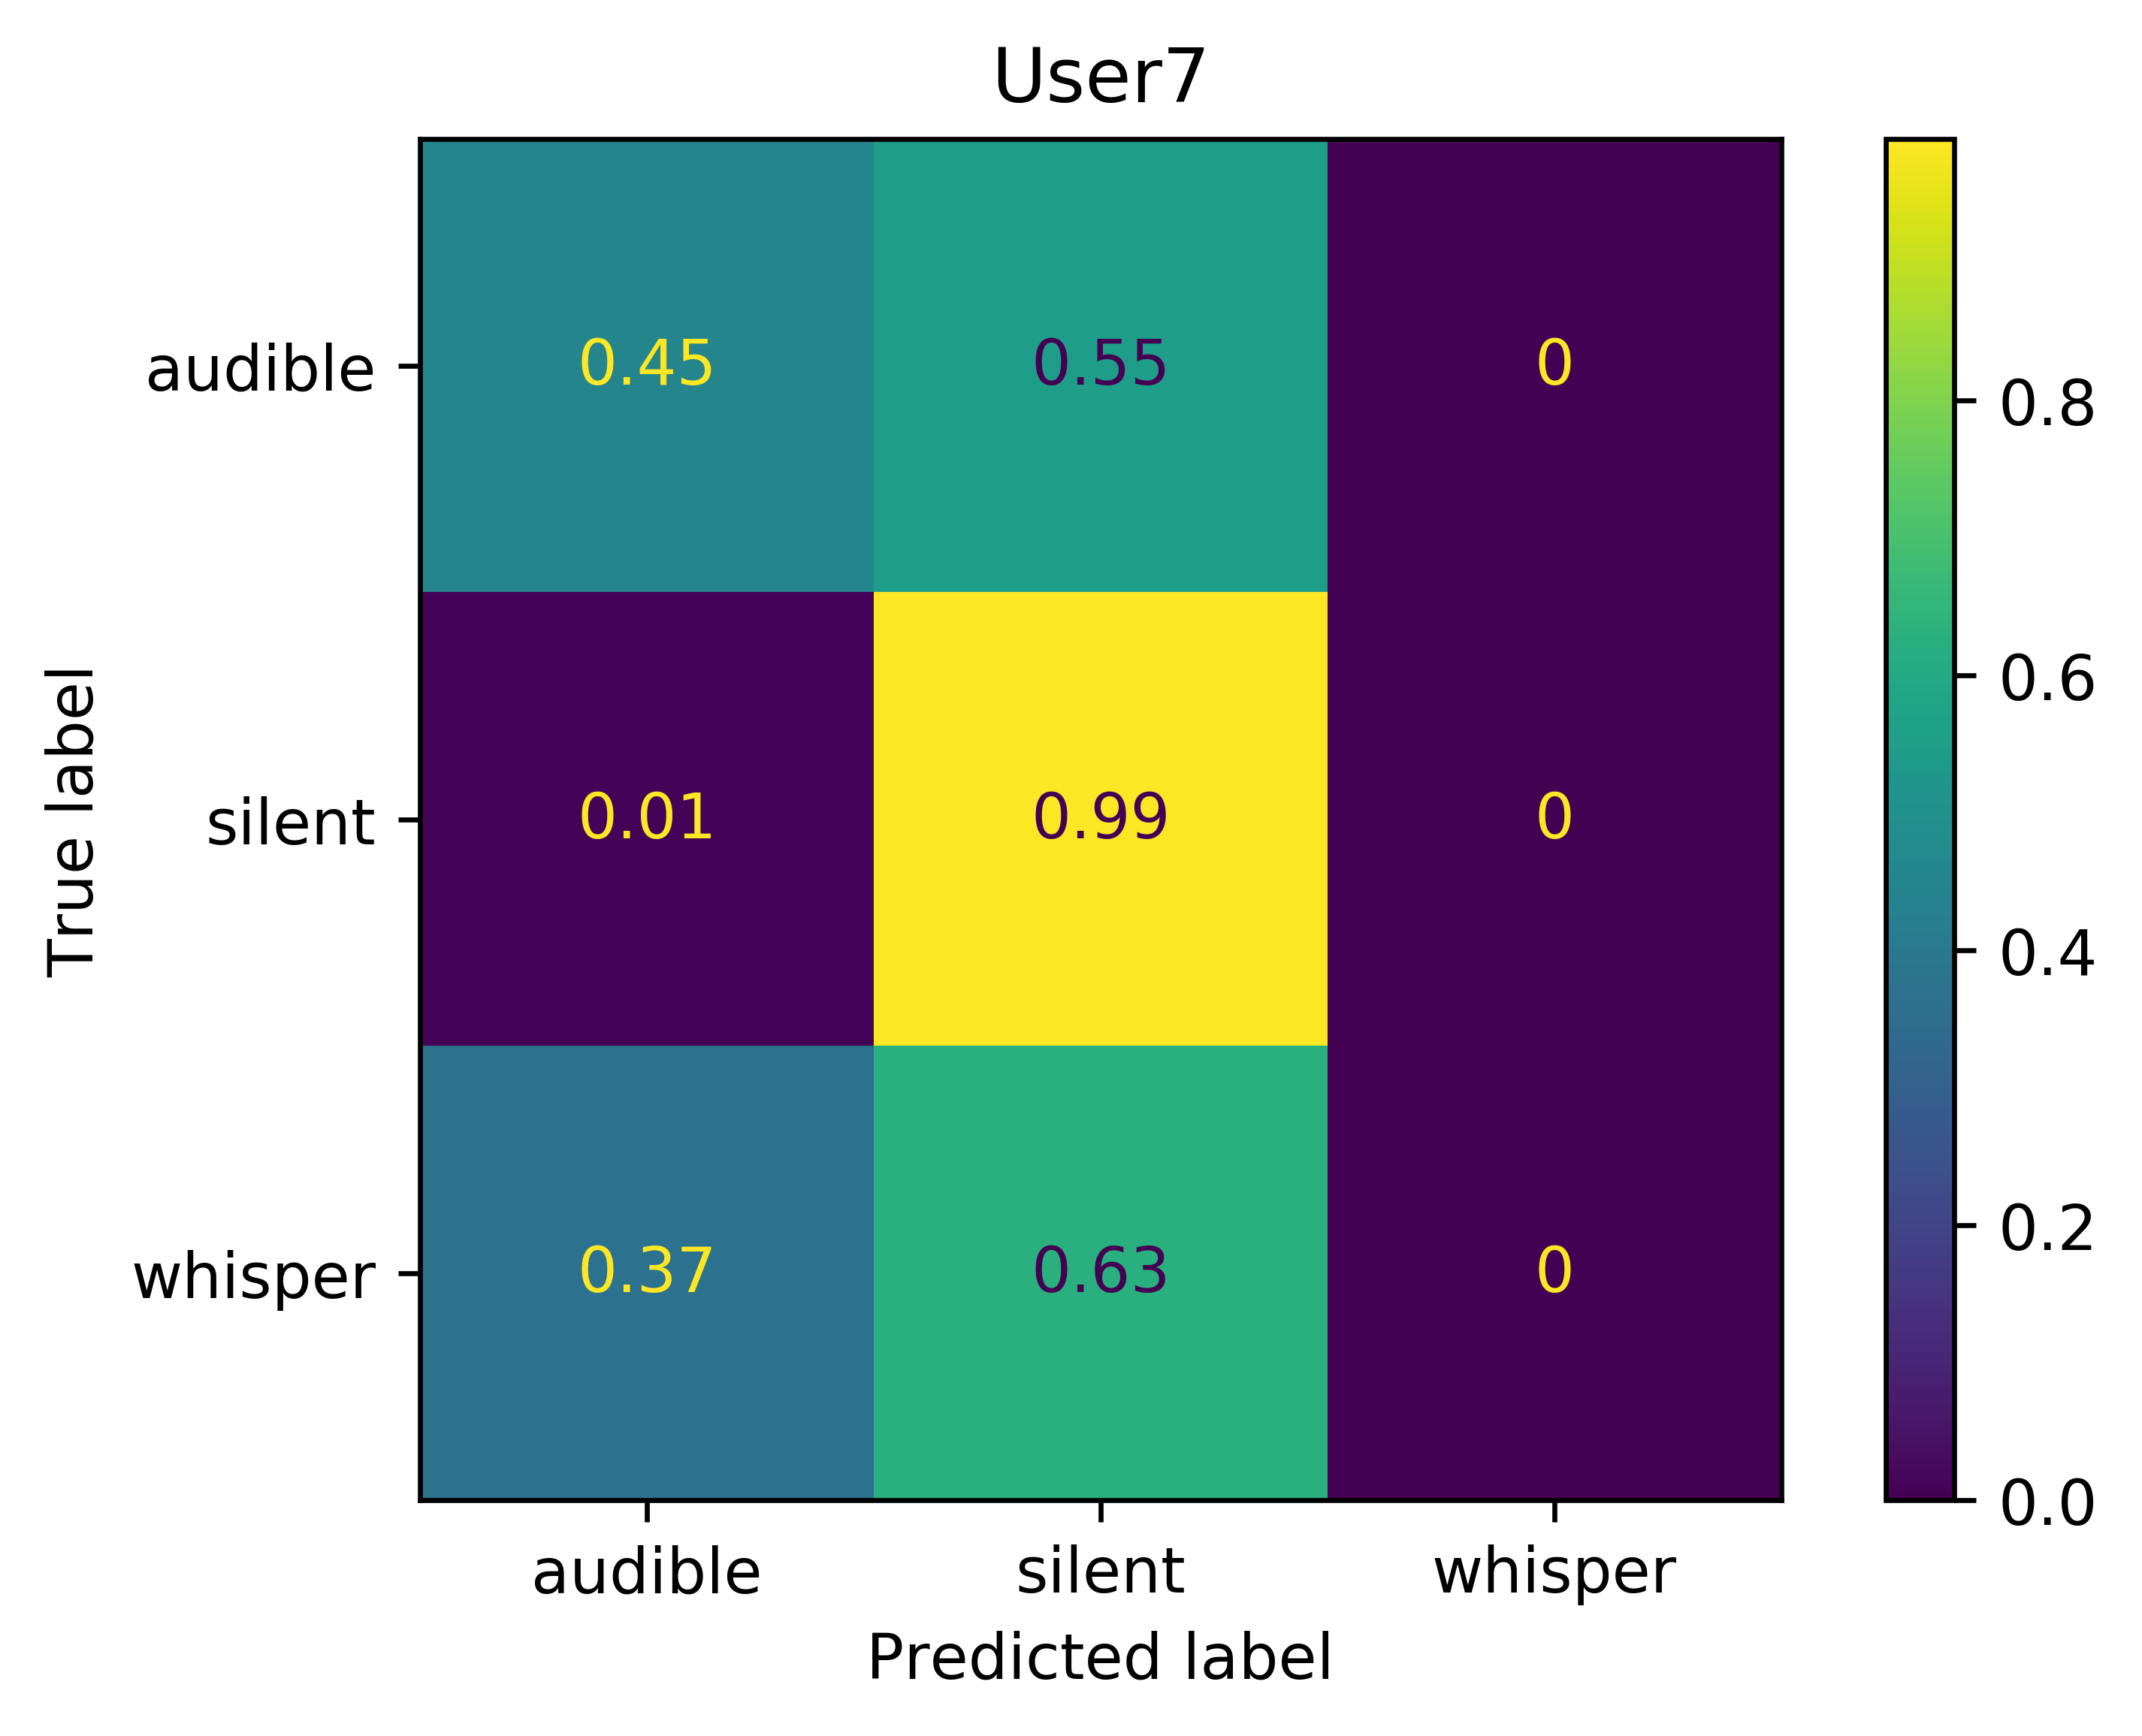
\includegraphics[width=63mm]{modeCrossUserUnf/User7_unf.png}}
\subfigure[Sprecher 8]{\label{fig:cnf17}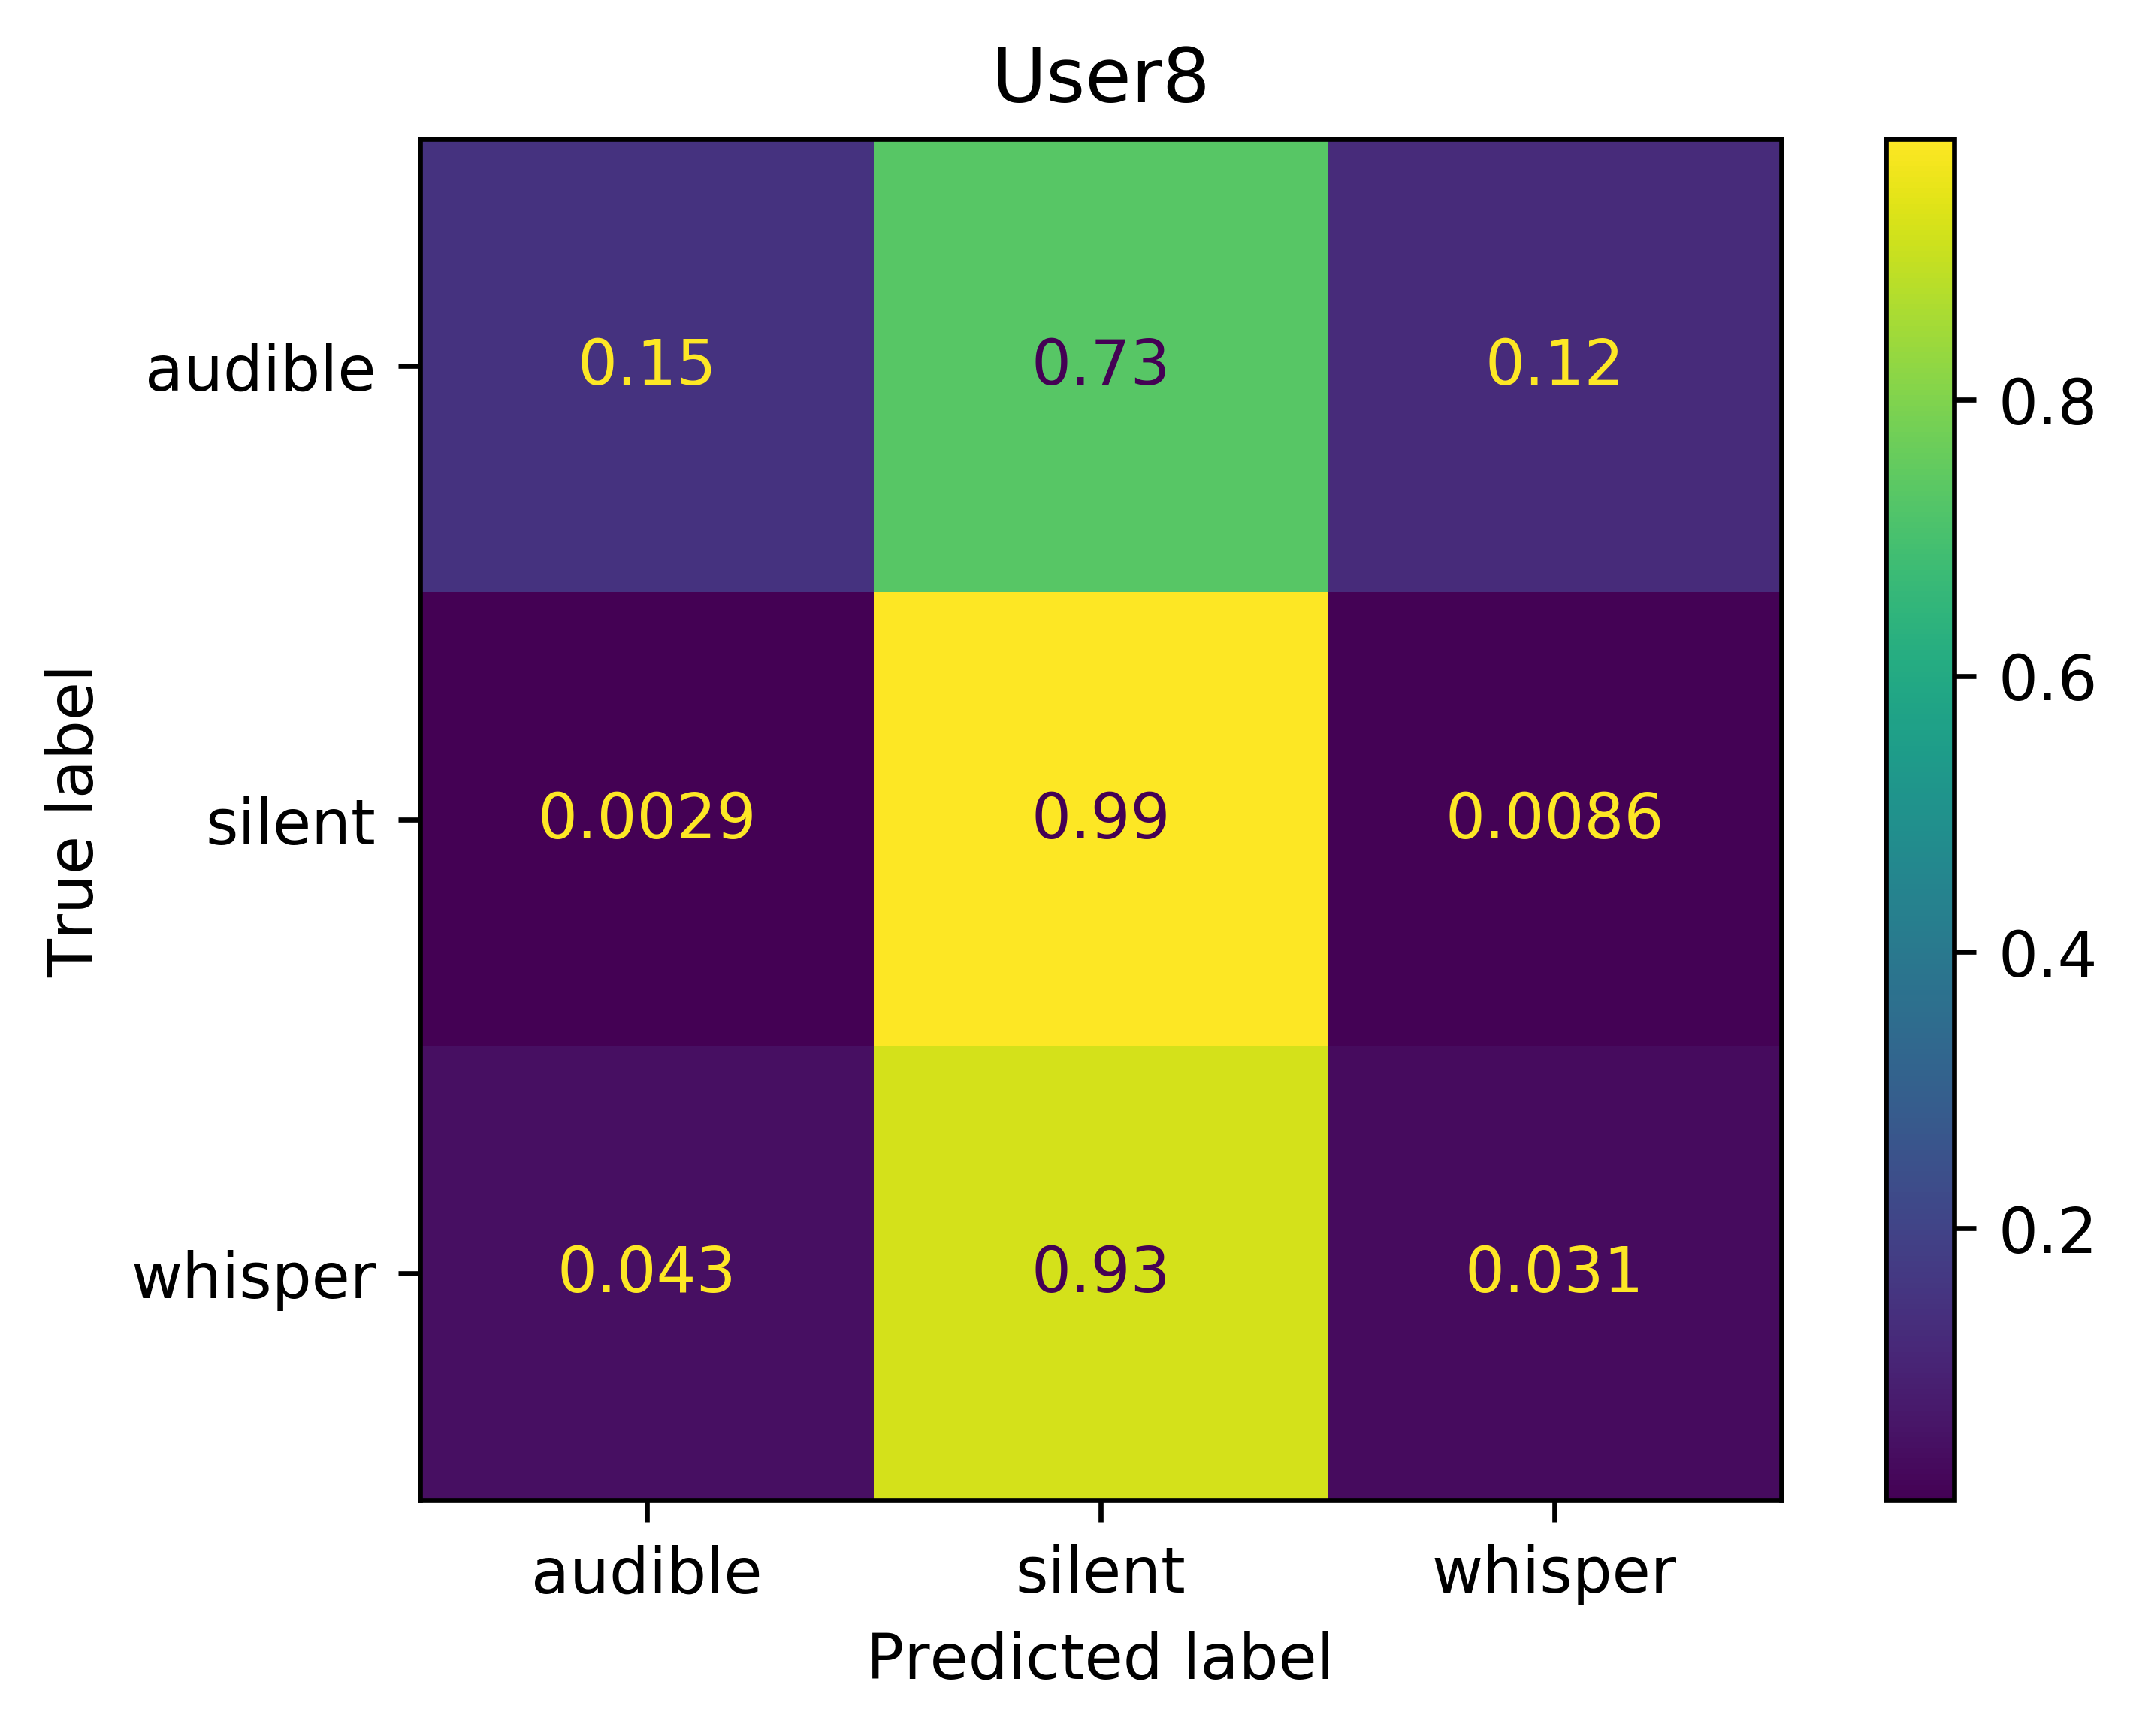
\includegraphics[width=63mm]{modeCrossUserUnf/User8_unf.png}}
\caption{Die Erkennungsraten der Sprecher  für die Vorhersage des Sprachmodus mit ungefilterten Daten.}
\label{fig:cnfsunfiltered}
\end{figure}

\subsubsection{Filtered}
Hier(\ref{fig:mode5}) wurde der selbe Bandpassfilter auf die Daten angewendet wie in dem Sprachmodus. Es ist eine ähnliche Verteilung der Genauigkeit wie in (\ref{fig:mode1}) zu betrachten wobei der Lda, der Randomforest sowie der LinerSVC die höchsten Werte vorweisen und der LDA-Klassfikator mit 49.13 Prozent die höchste Genauigkeit bietet. Der KNN-Klassifikator hat die niedrigste Genauigkeit mit 38.78 Prozent. Es lässt sich eine allgemein niedrigere Genauigkeit als bei der ungefilterten Variante in \ref{fig:mode4} beobachten.

\begin{figure}[H]
  \centering
  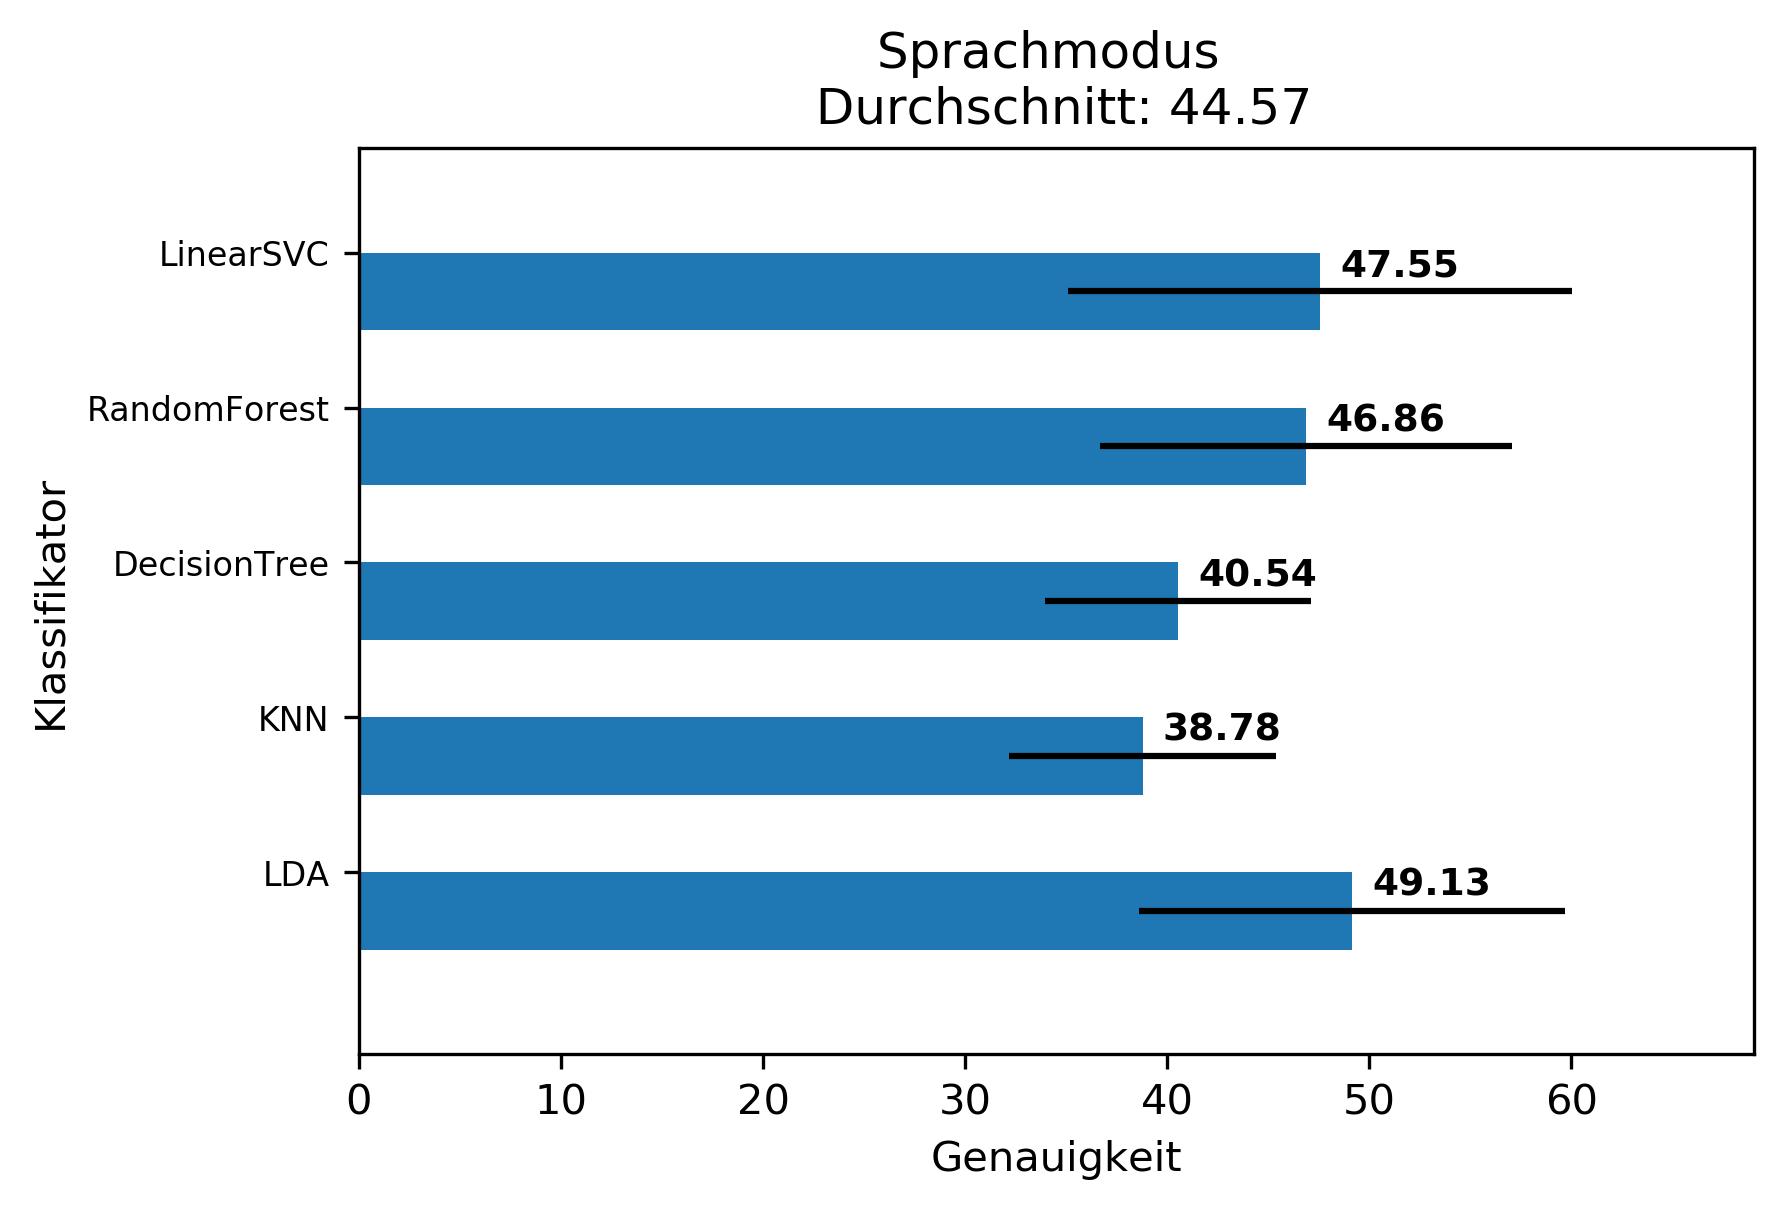
\includegraphics[width=100mm ,scale=0.6]{modeResultsUser10too200hz.png}
  \caption{Die durchschnittliche Genauigkeit, sowie die Standardabweichung der verschiedener Klassifikatoren bei der Erkennung des Sprachmodus.Hier werden die Daten aller Sprecher verwendet die mindestens 2 Sessions besitzen, also die Sprecher 1,2,4,7 und 8 zudem wurde ein 10-200hz filter verwendet.}
  \label{fig:mode5}
\end{figure}

\paragraph{}
Die Confusion-Matrix Analyse für die gefilterten Daten (\ref{fig:cnfsfiltered}) liefert identische Resultate zu den ungefilterten Resultaten.

\begin{figure}[H]
\centering     %%% not \center
\subfigure[Sprecher 1]{\label{fig:cnf18}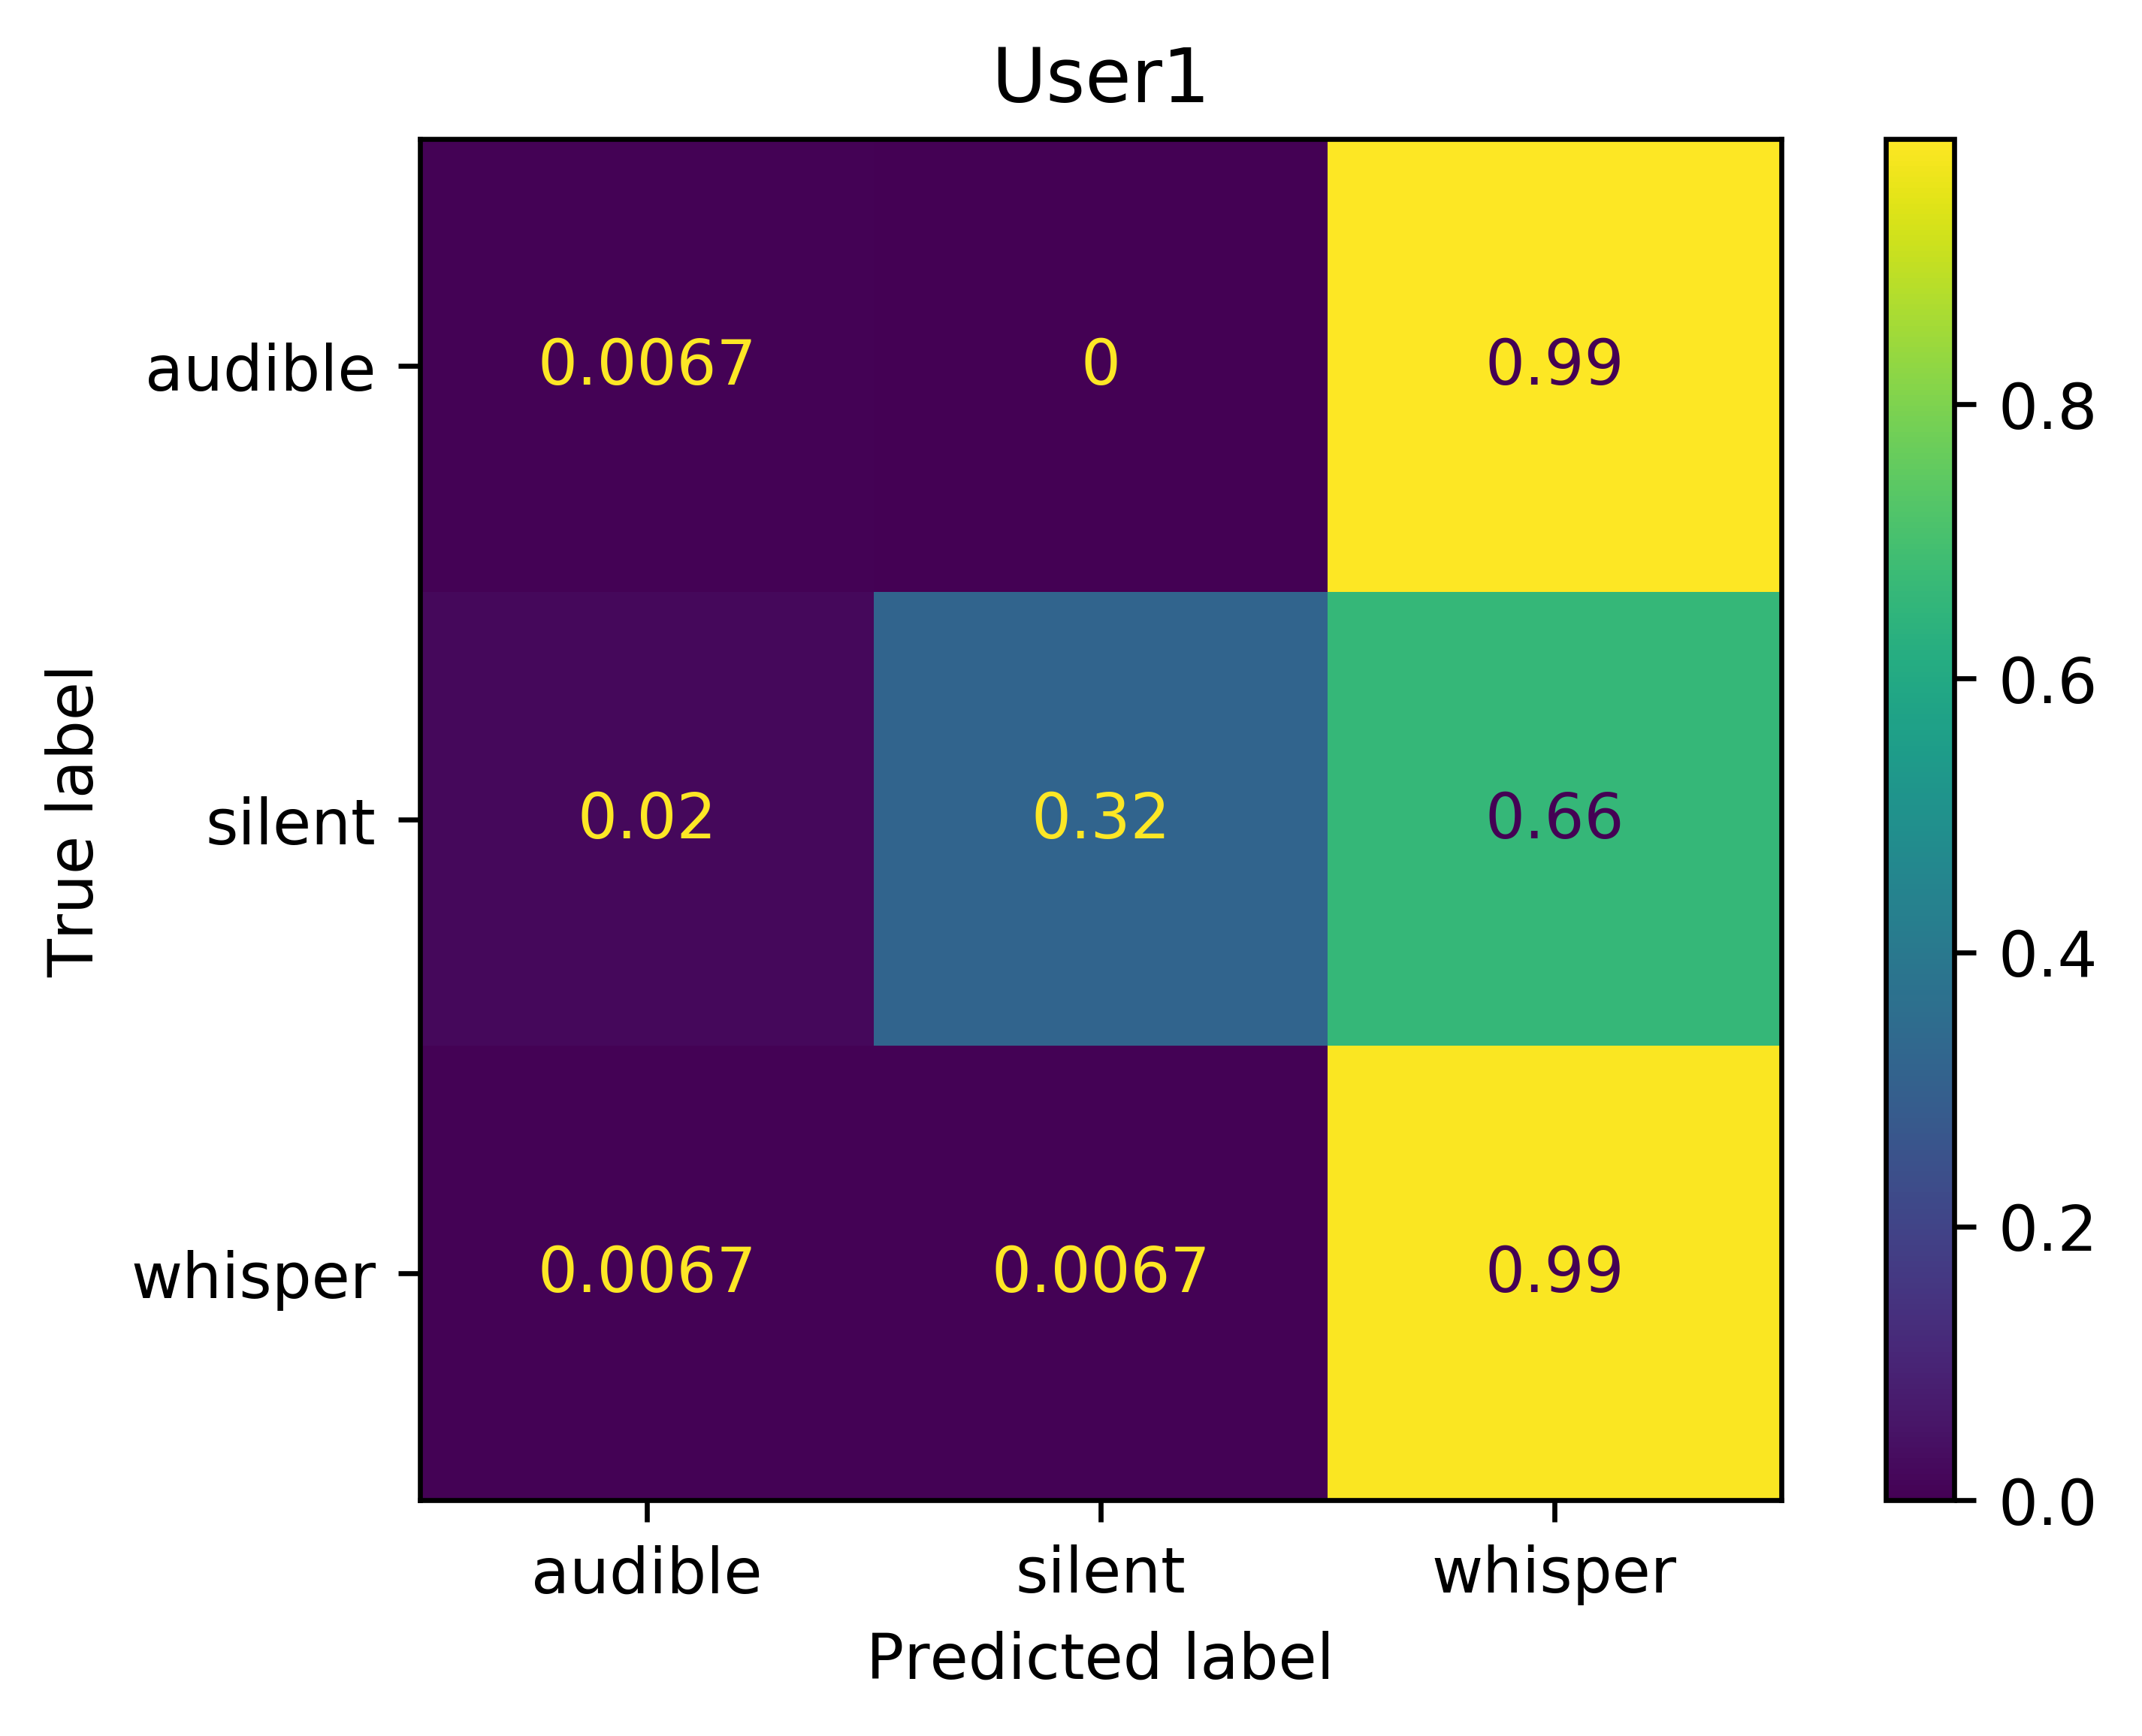
\includegraphics[width=63mm]{modeCrossUser/User1.png}}
\subfigure[Sprecher 2]{\label{fig:cnf19}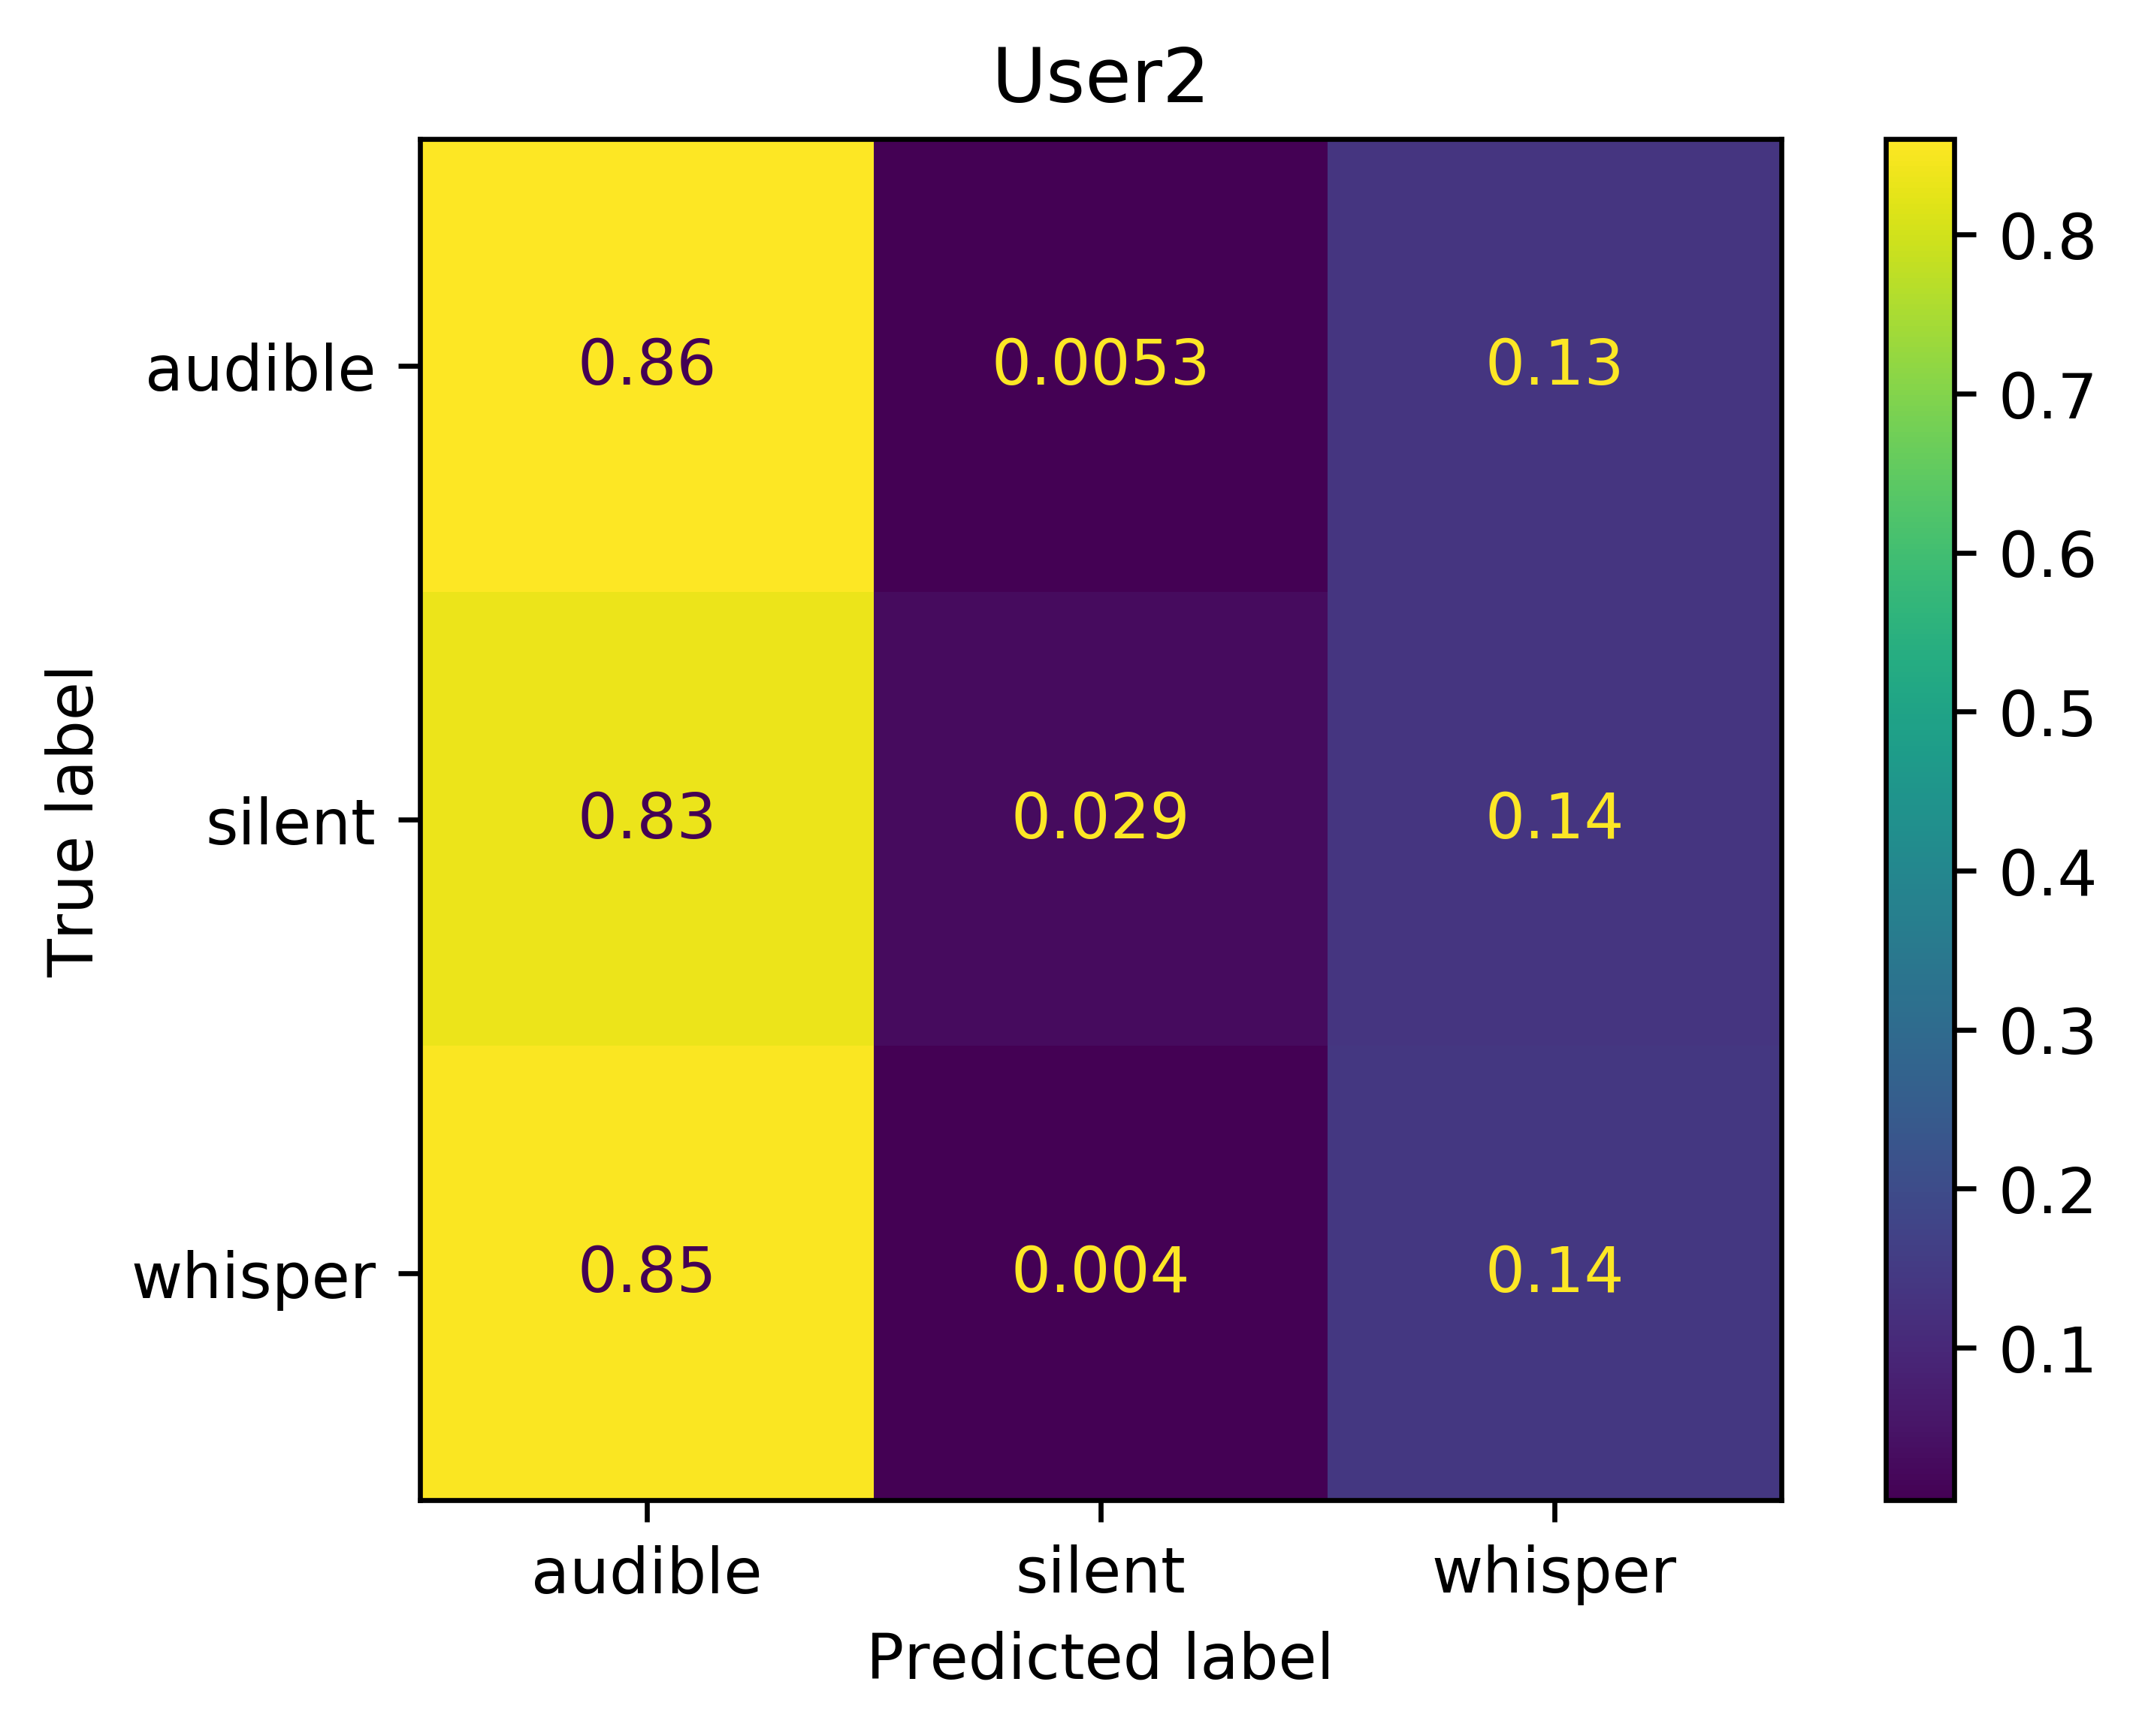
\includegraphics[width=63mm]{modeCrossUser/User2.png}}
\subfigure[Sprecher 3]{\label{fig:cnf20}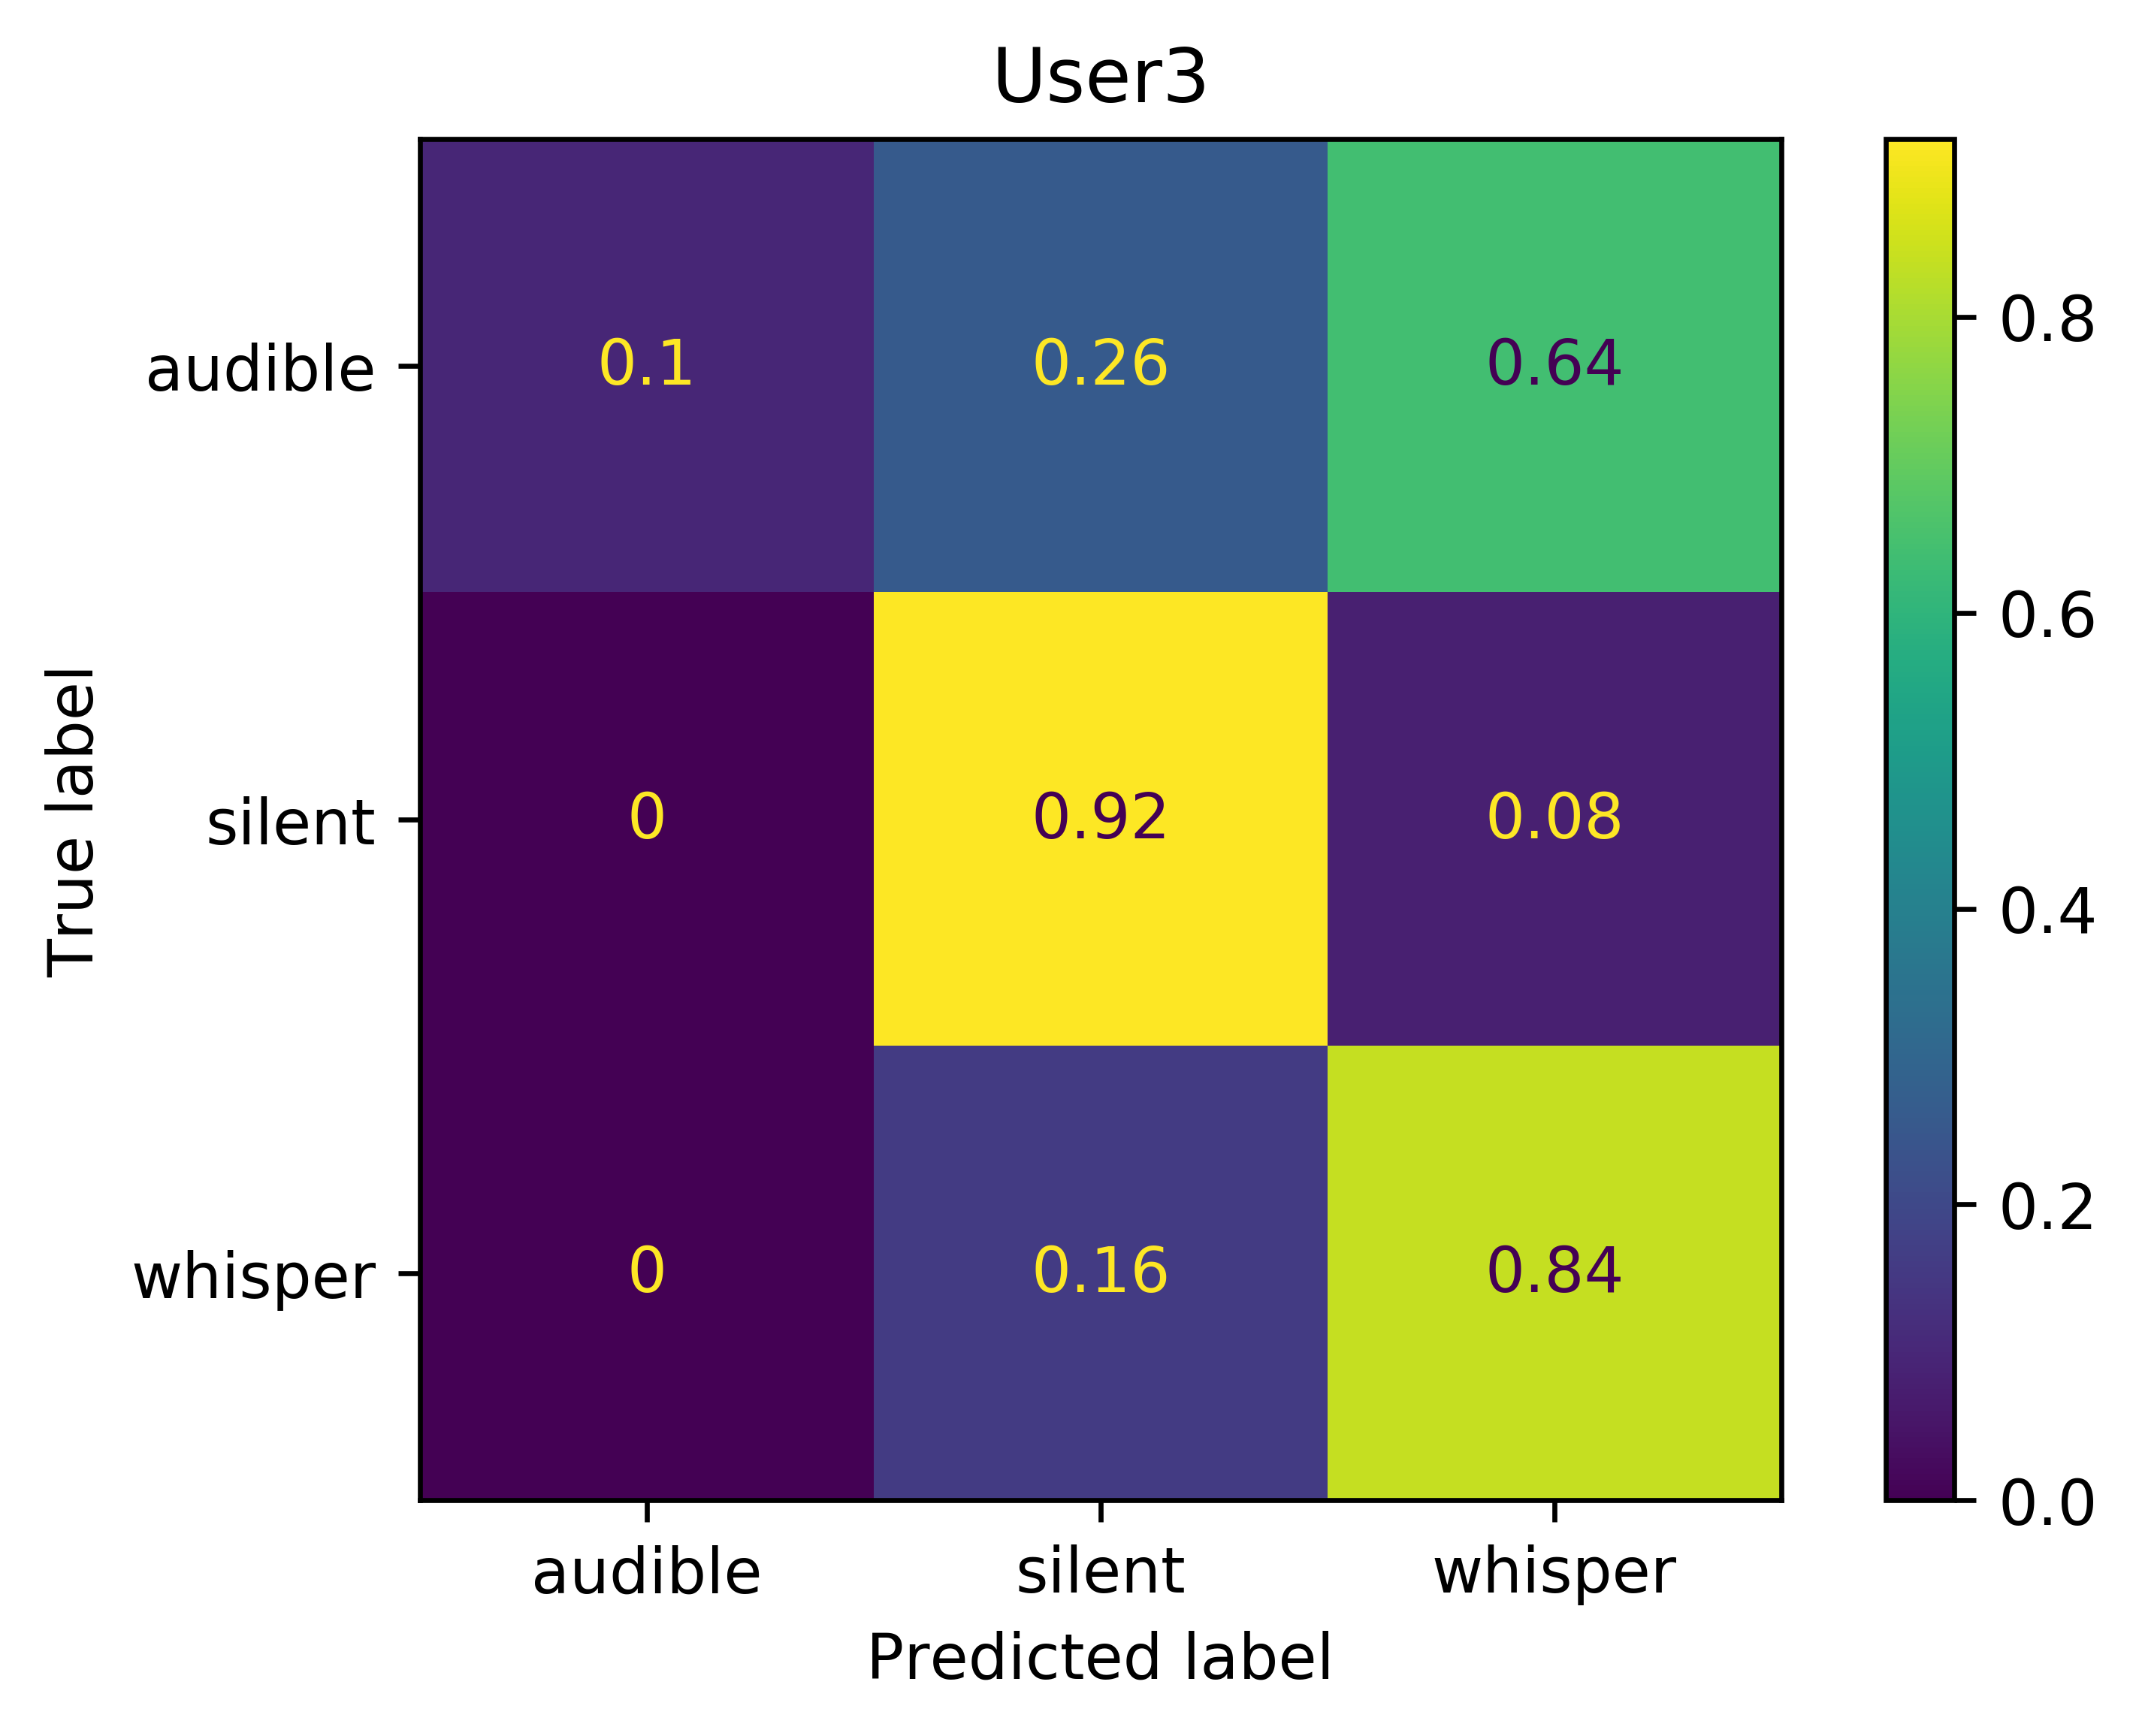
\includegraphics[width=63mm]{modeCrossUser/User3.png}}
\subfigure[Sprecher 4]{\label{fig:cnf21}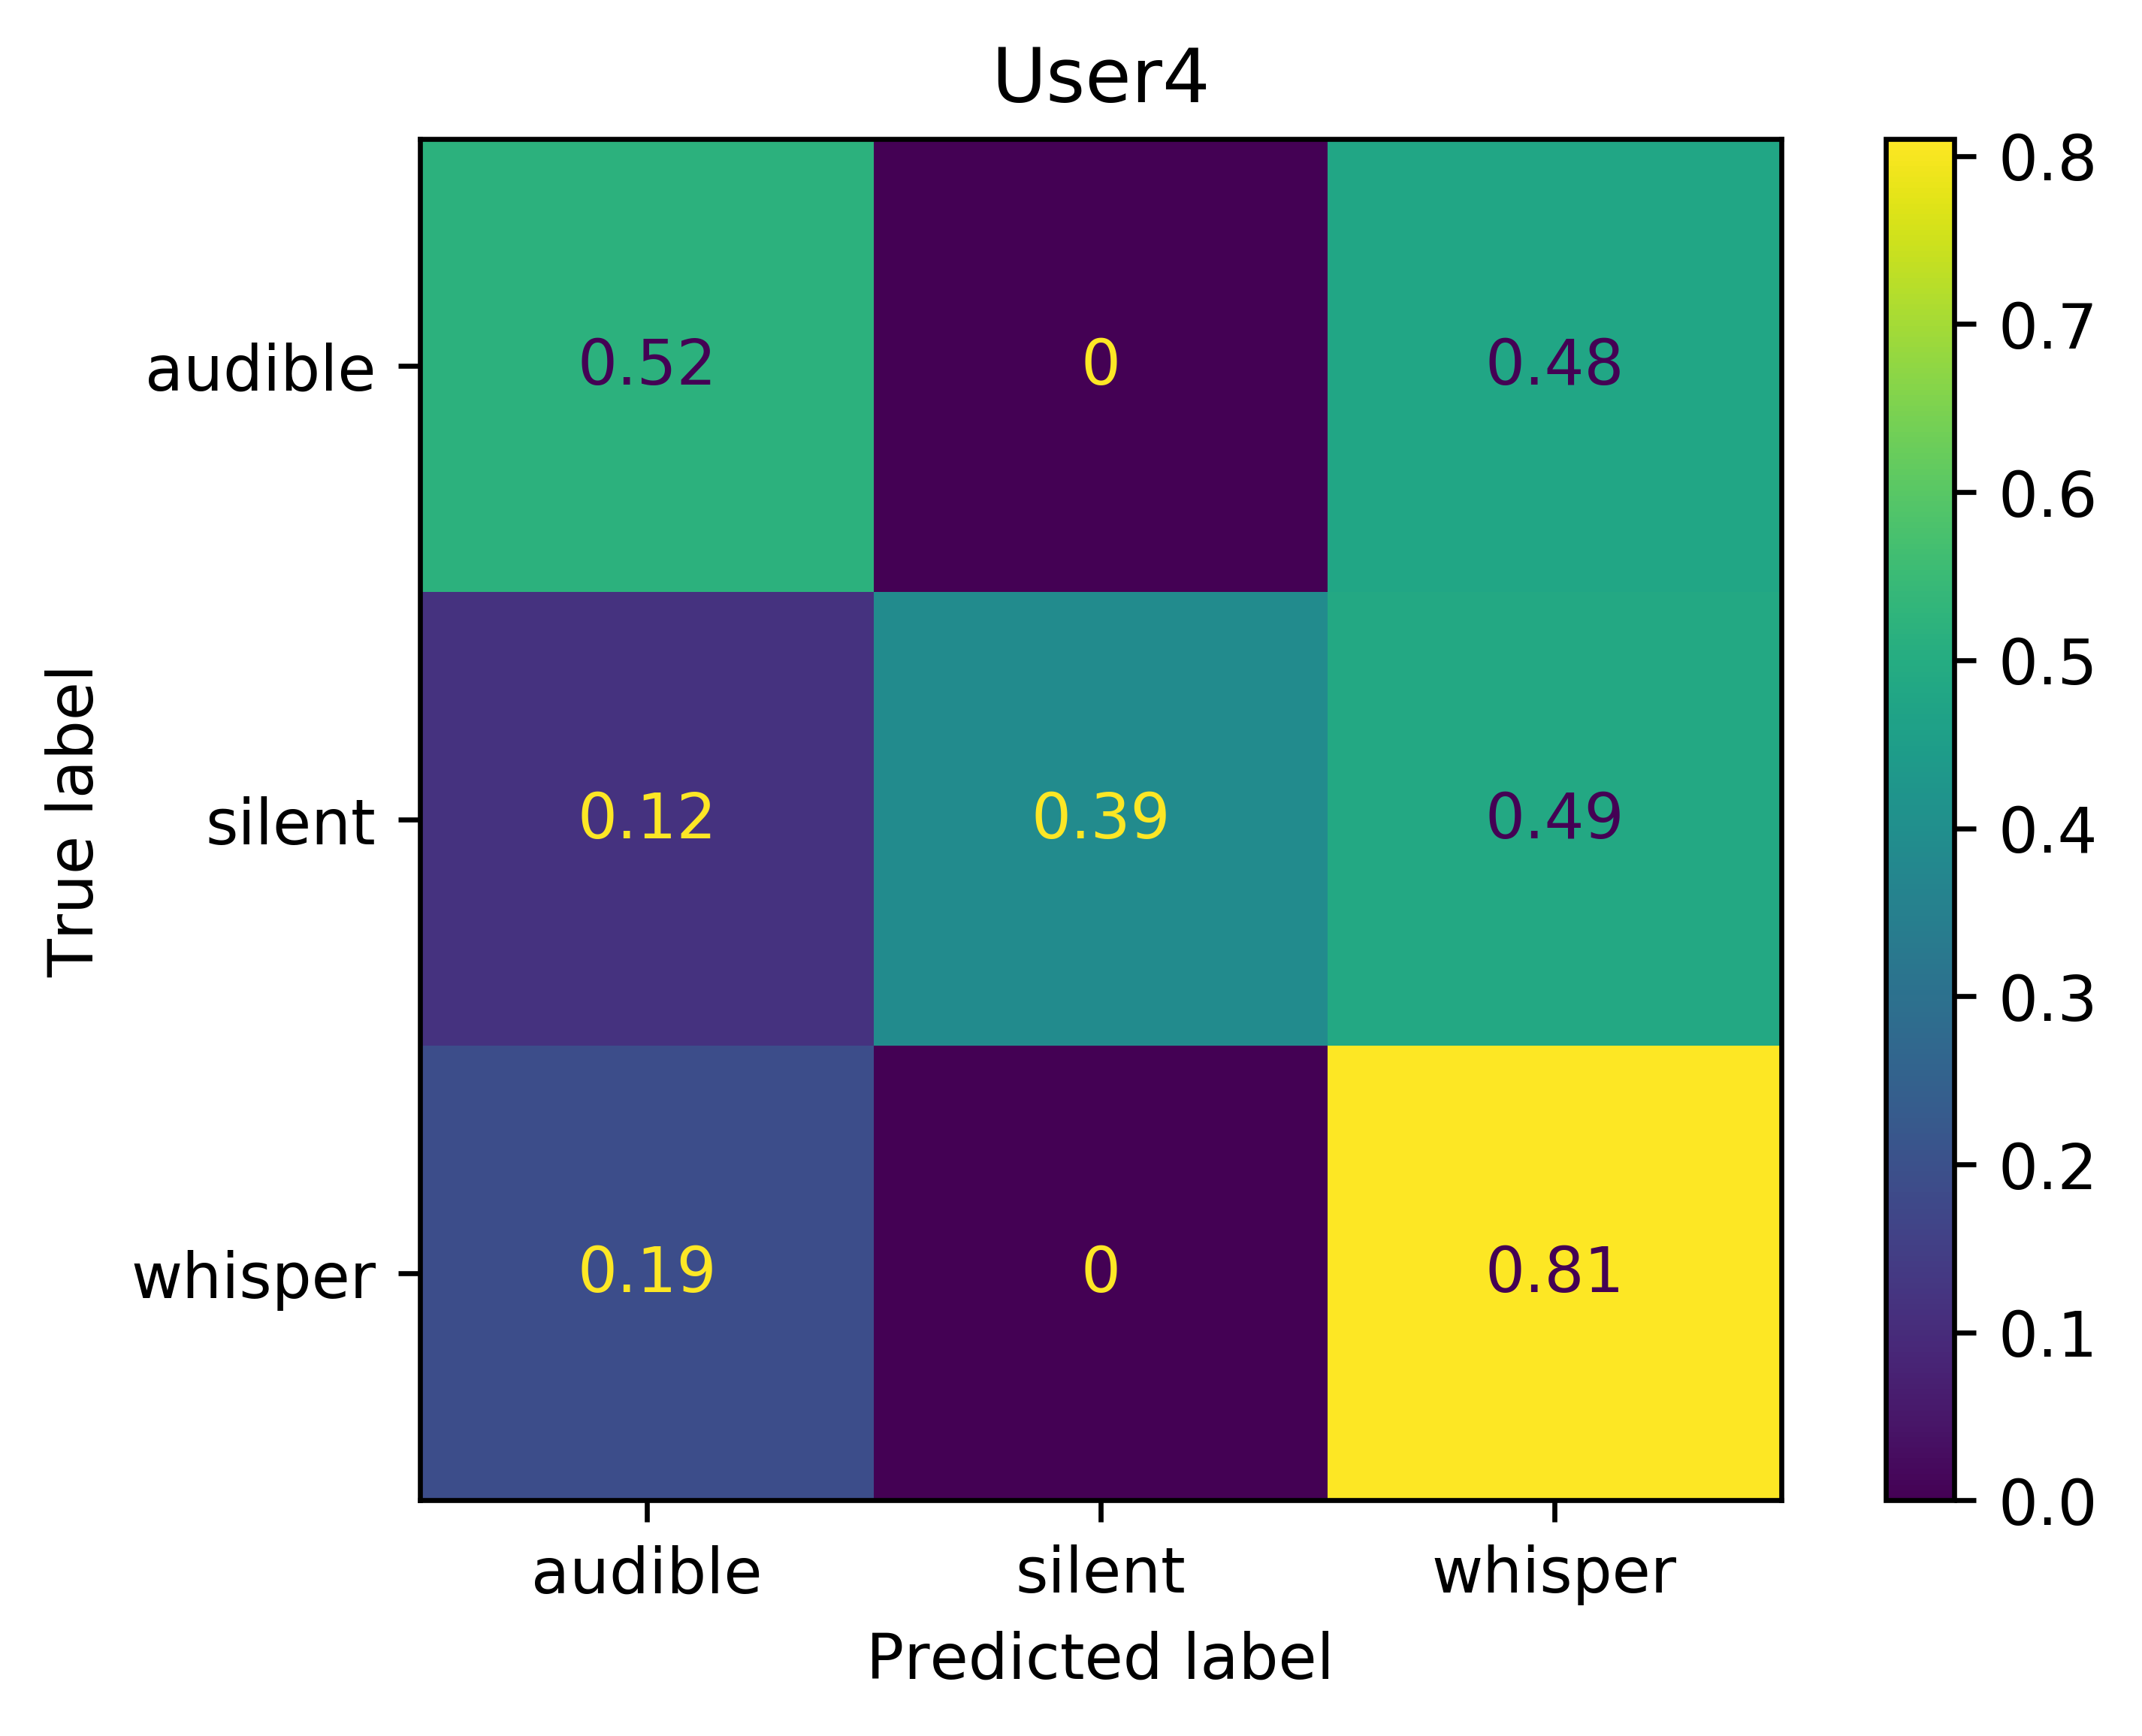
\includegraphics[width=63mm]{modeCrossUser/User4.png}}
\subfigure[Sprecher 5]{\label{fig:cnf22}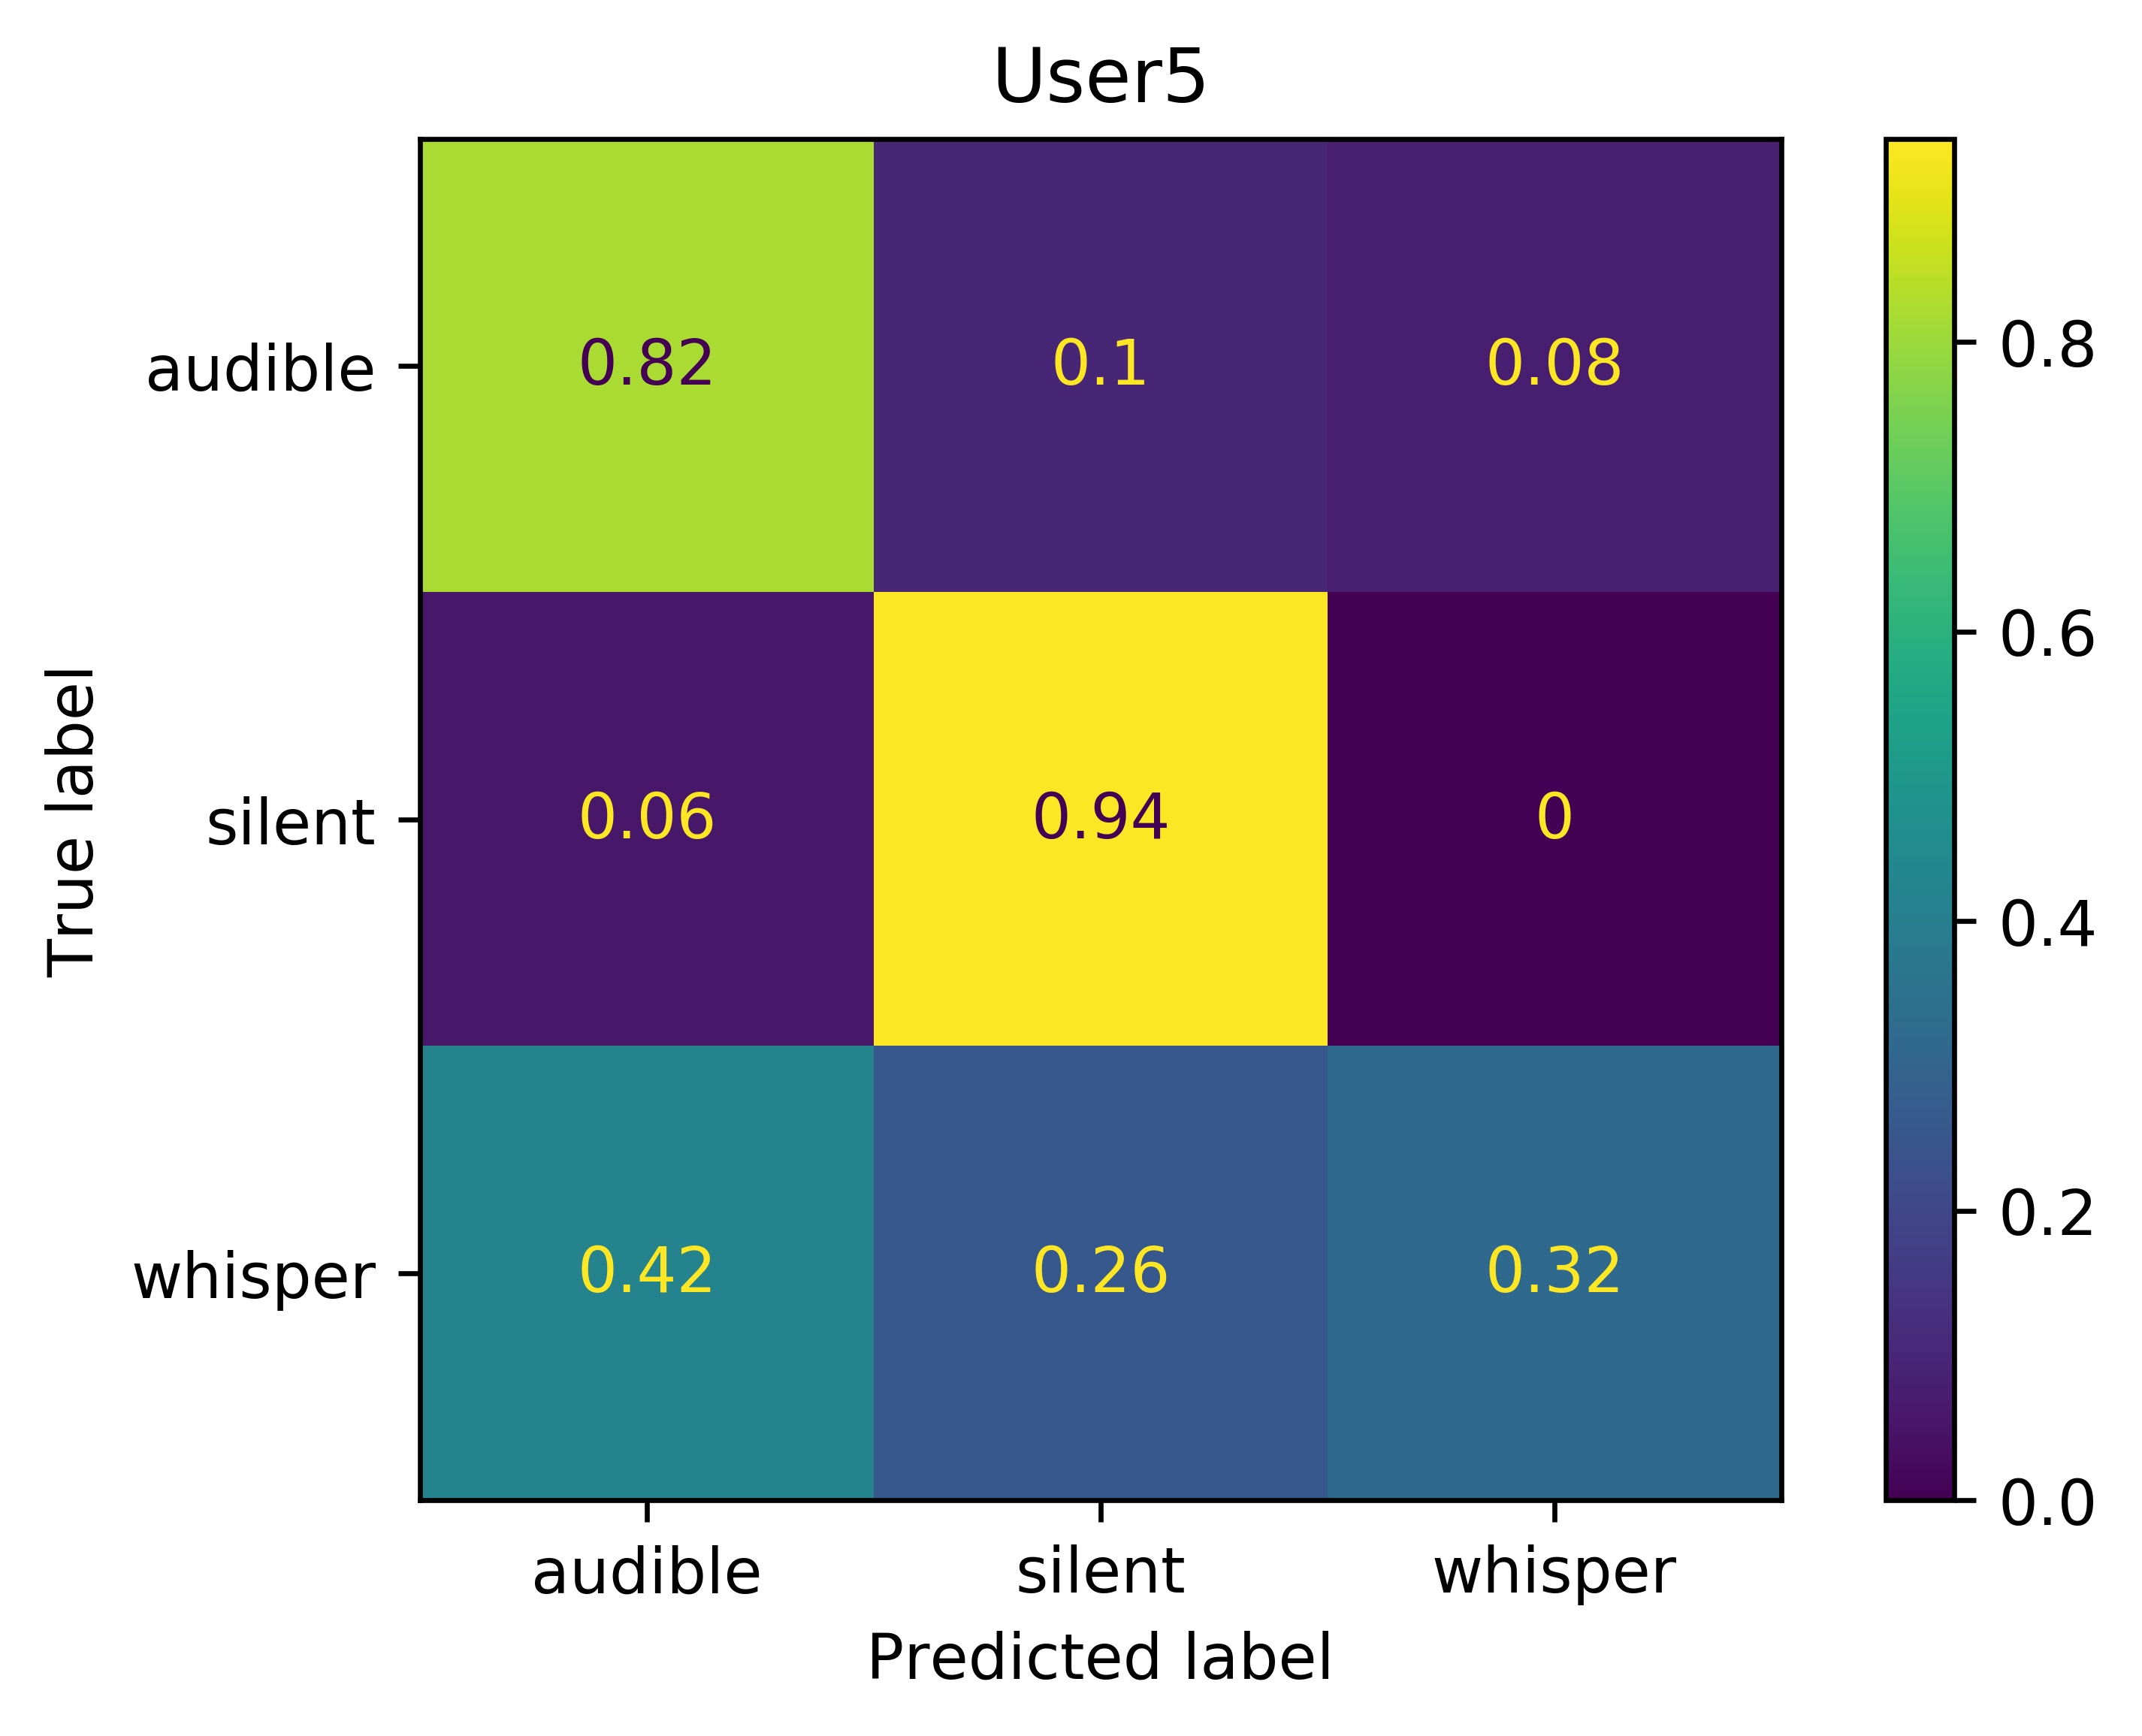
\includegraphics[width=63mm]{modeCrossUser/User5.png}}
\subfigure[Sprecher 6]{\label{fig:cnf23}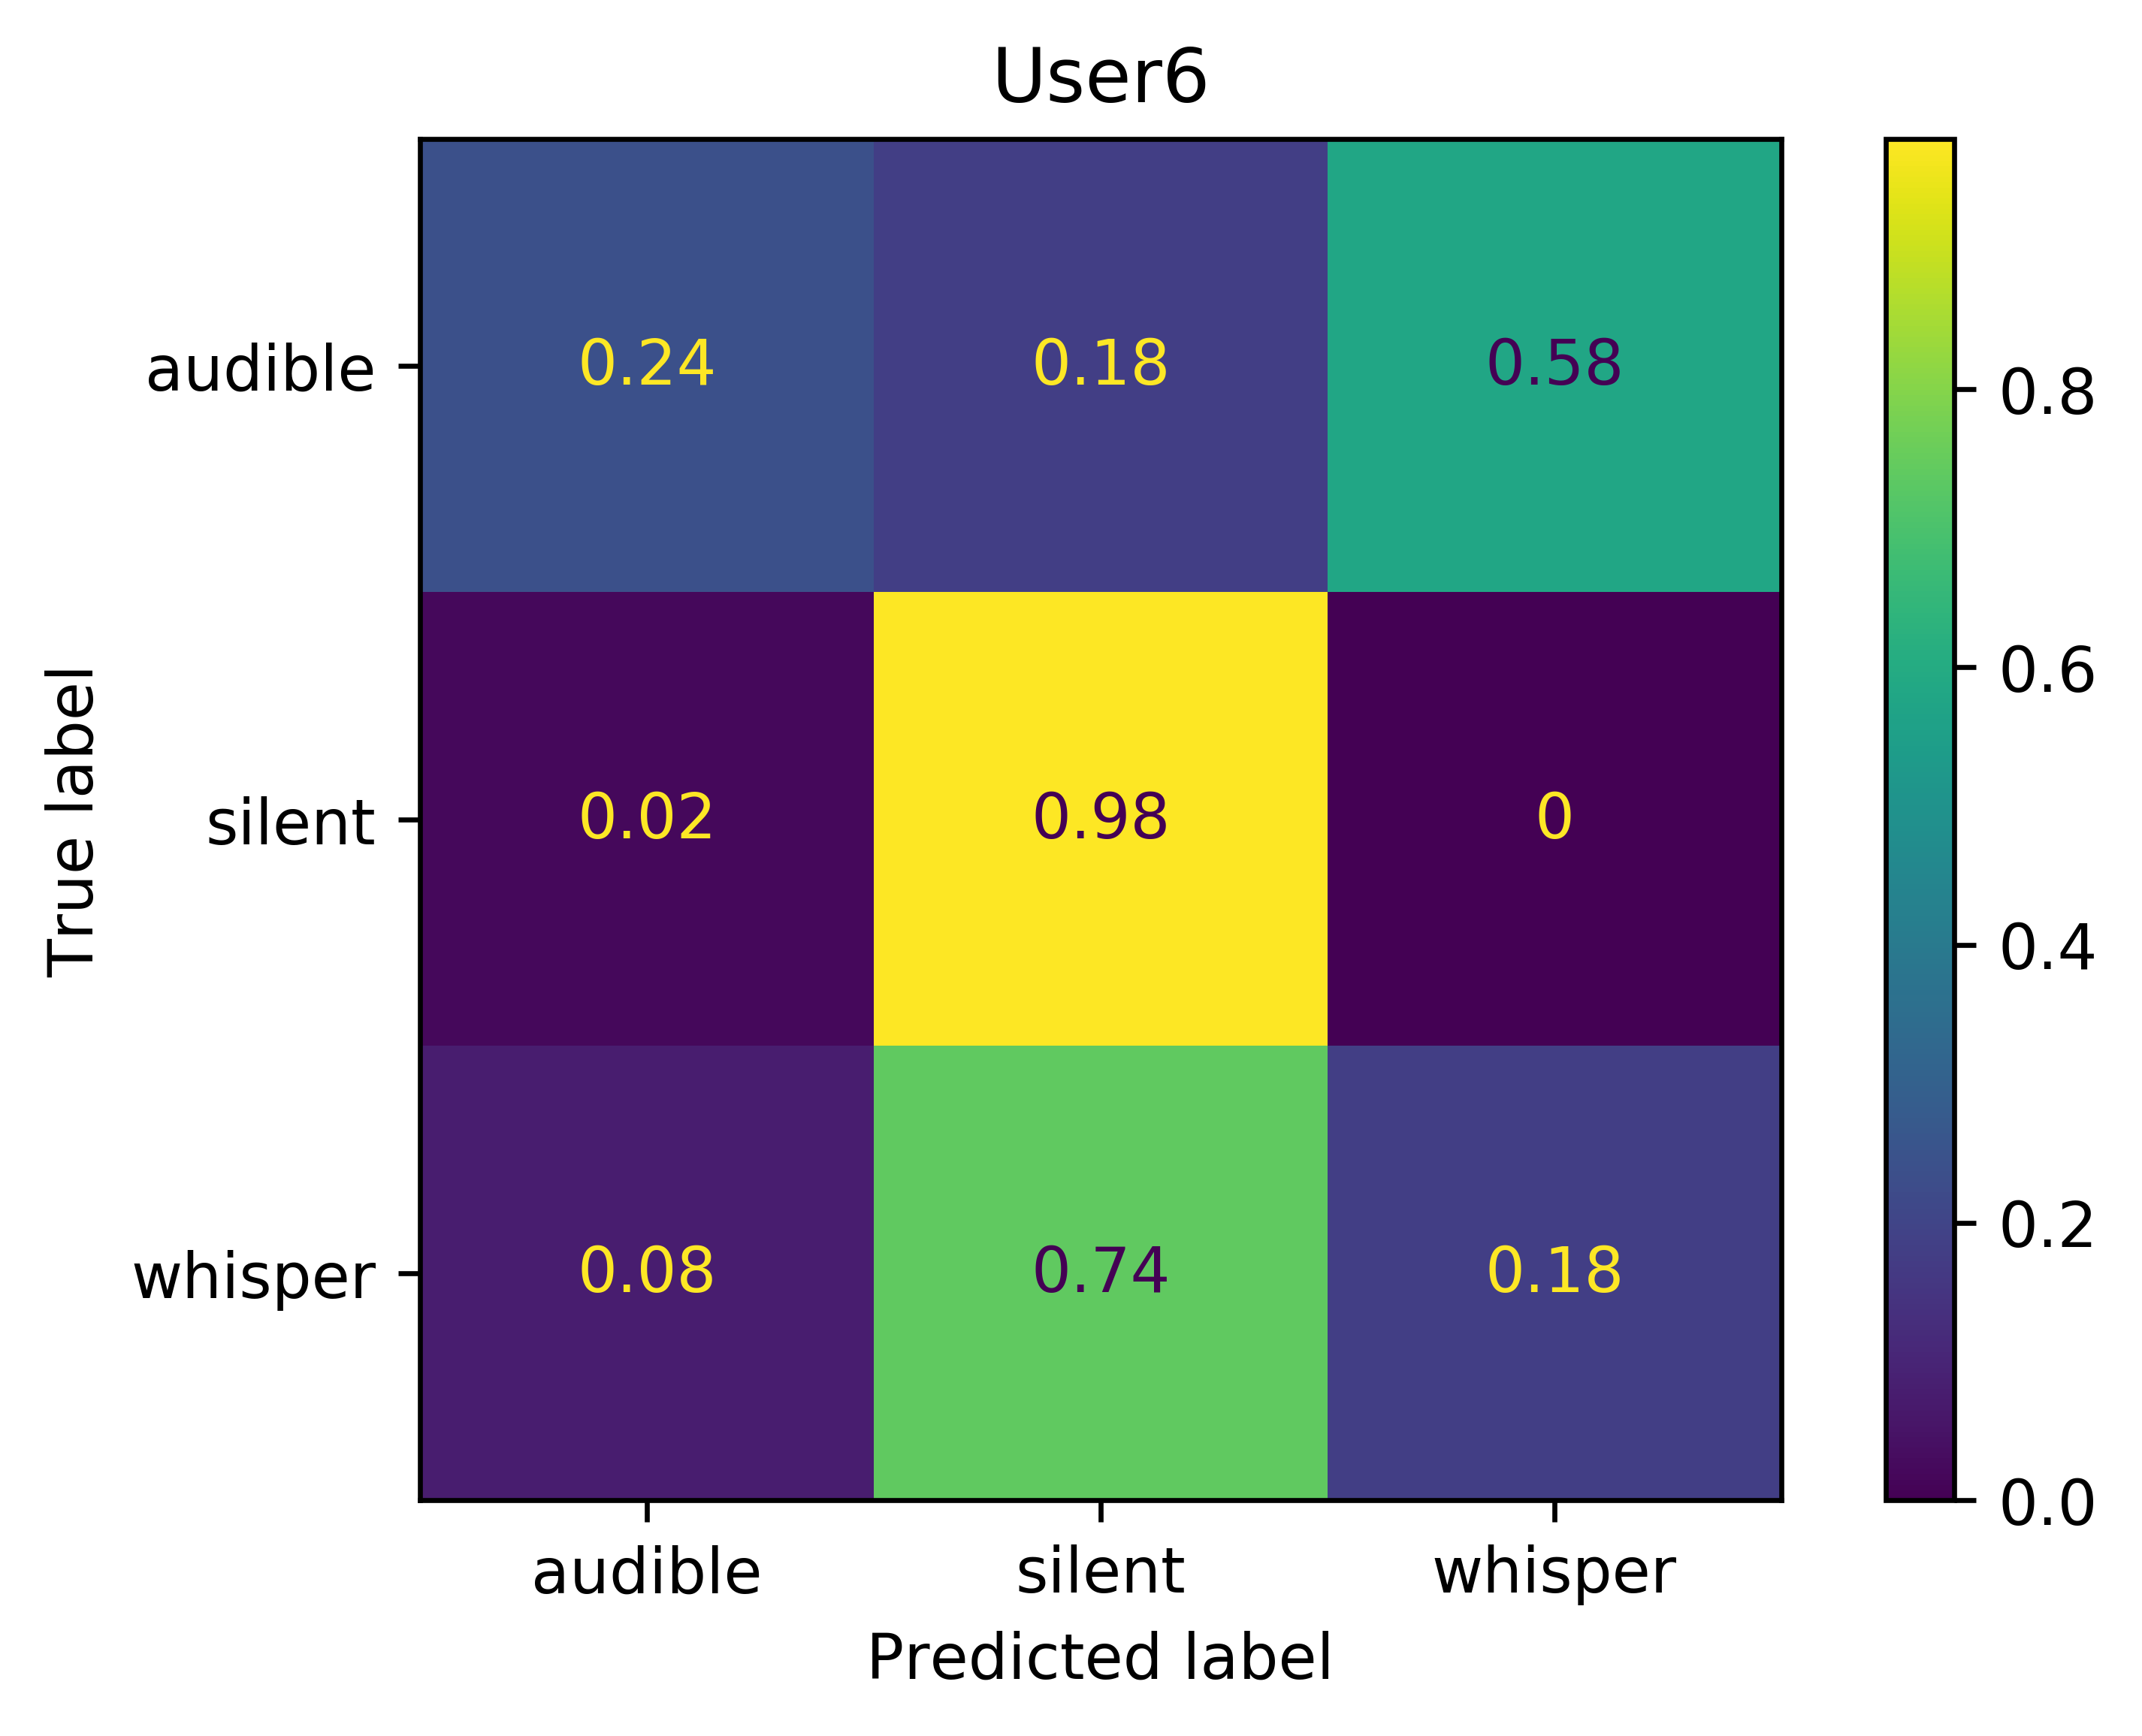
\includegraphics[width=63mm]{modeCrossUser/User6.png}}
\subfigure[Sprecher 7]{\label{fig:cnf24}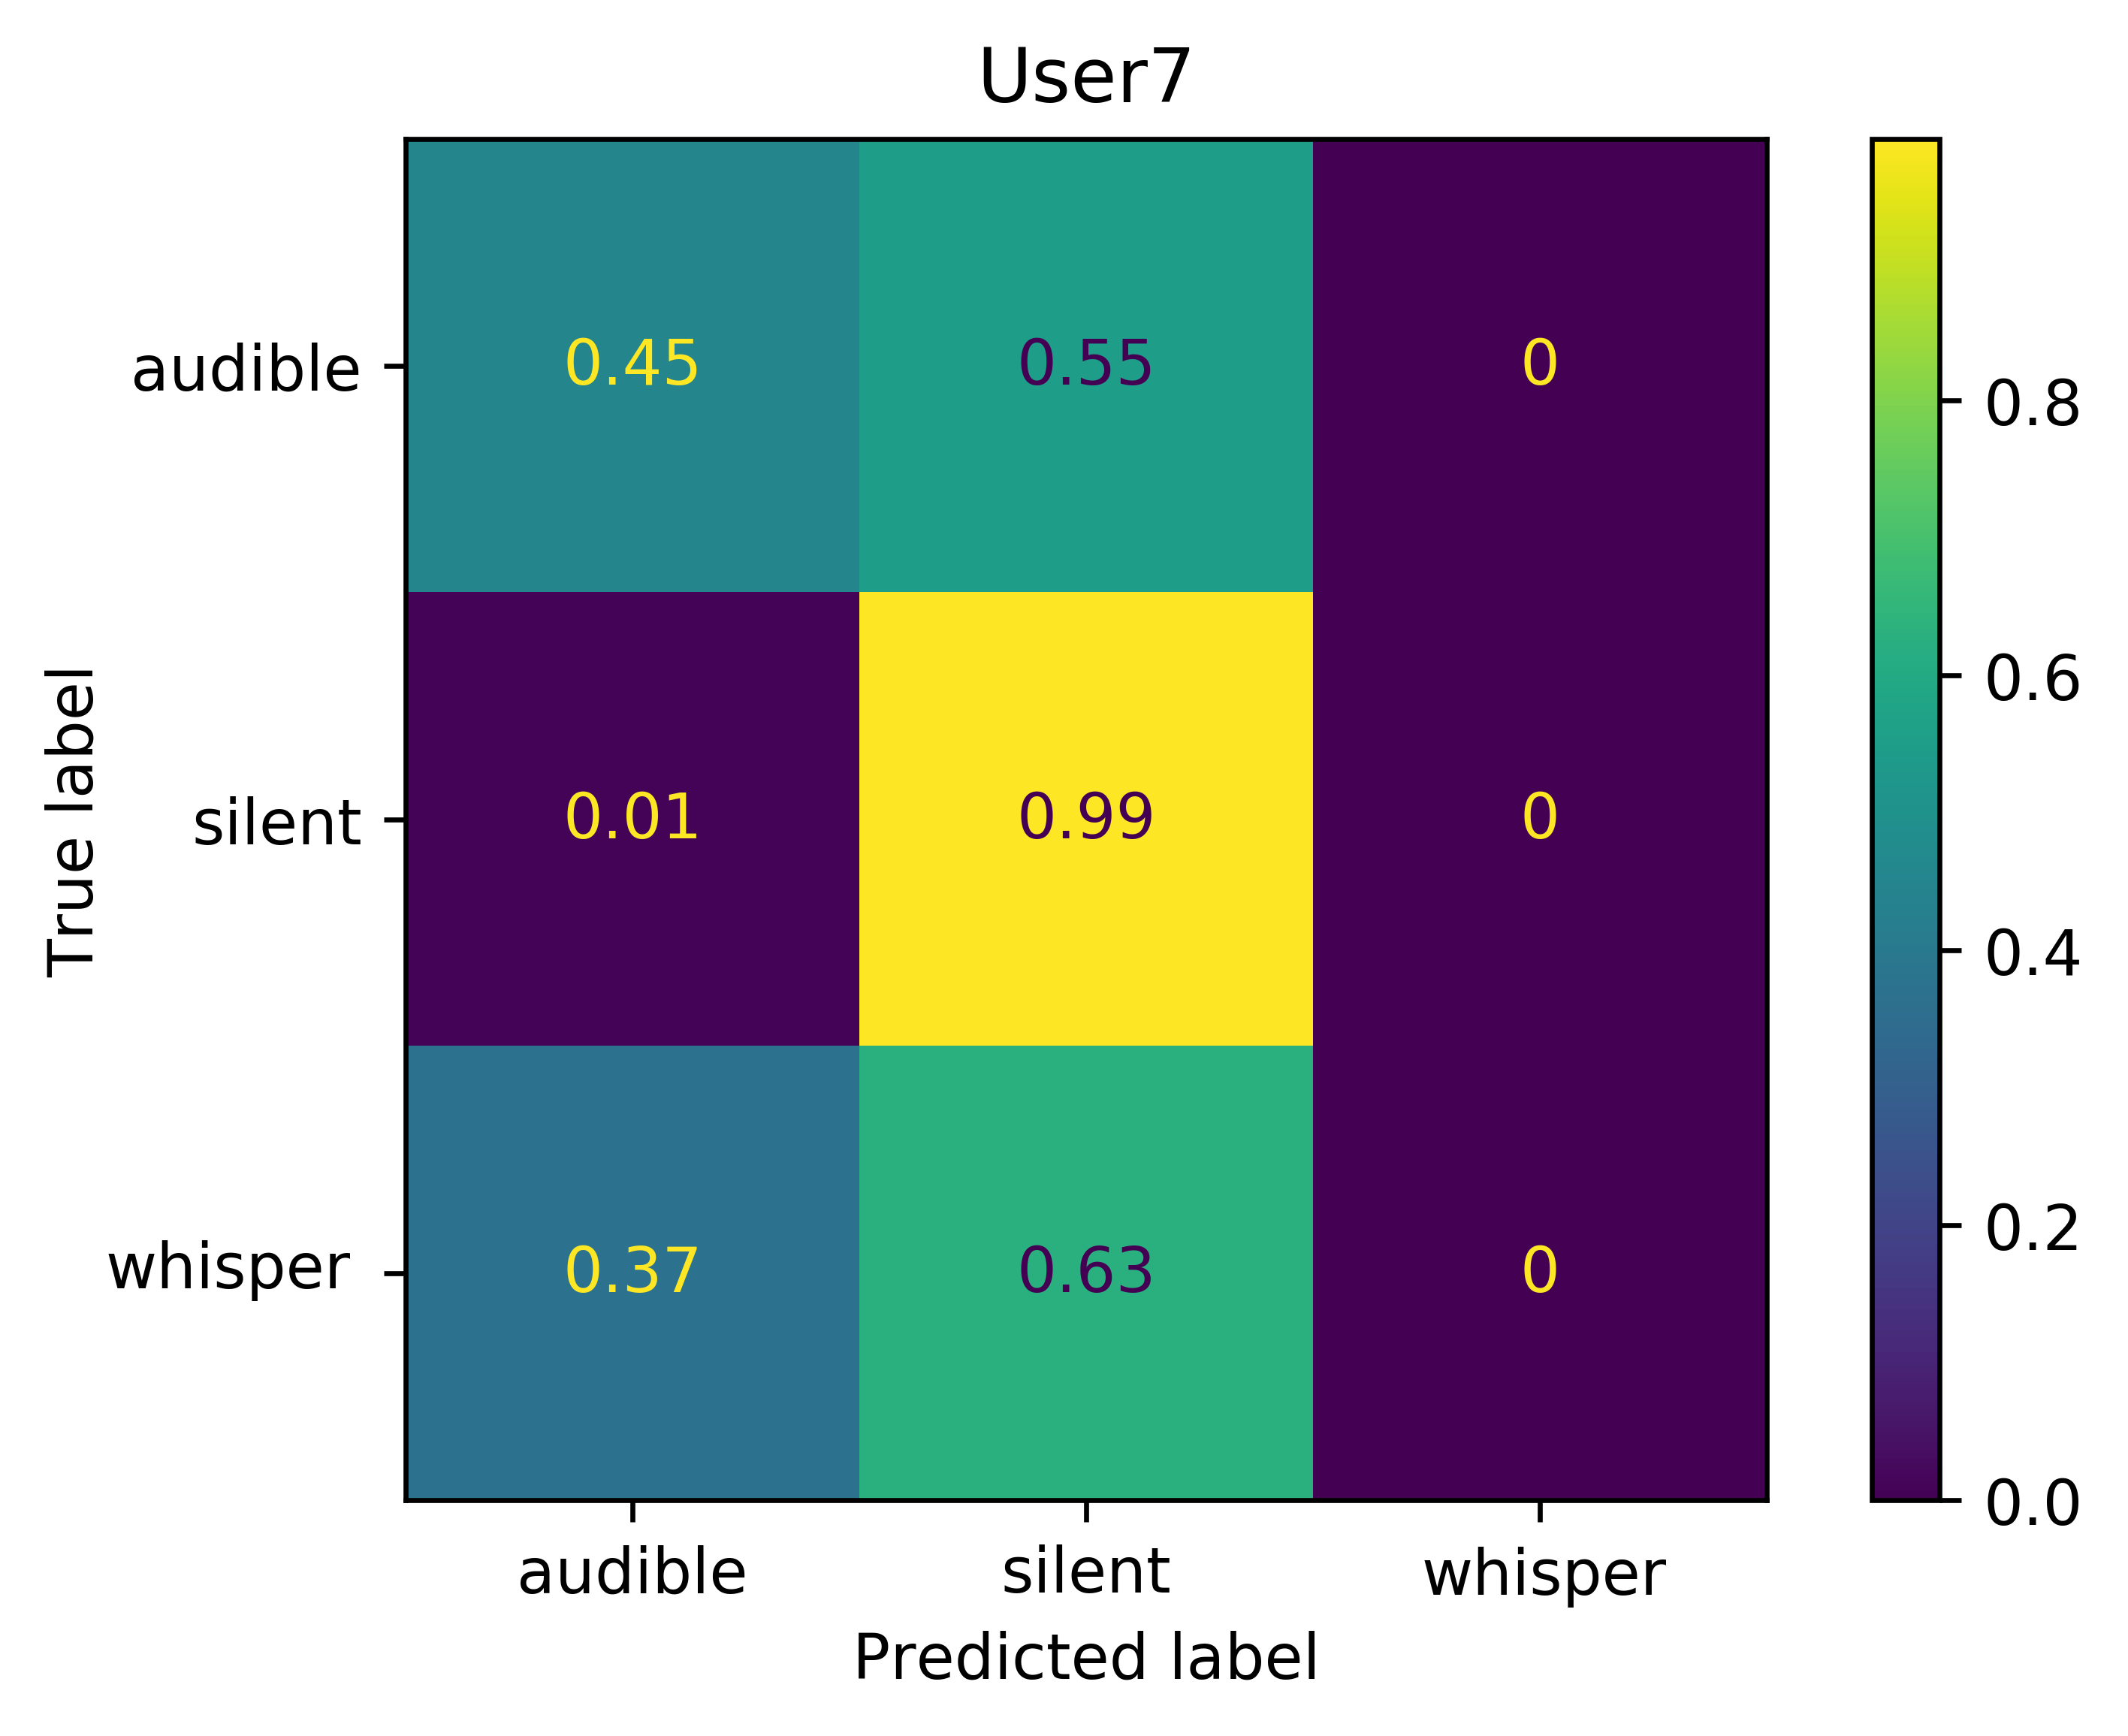
\includegraphics[width=63mm]{modeCrossUser/User7.png}}
\subfigure[Sprecher 8]{\label{fig:cnf25}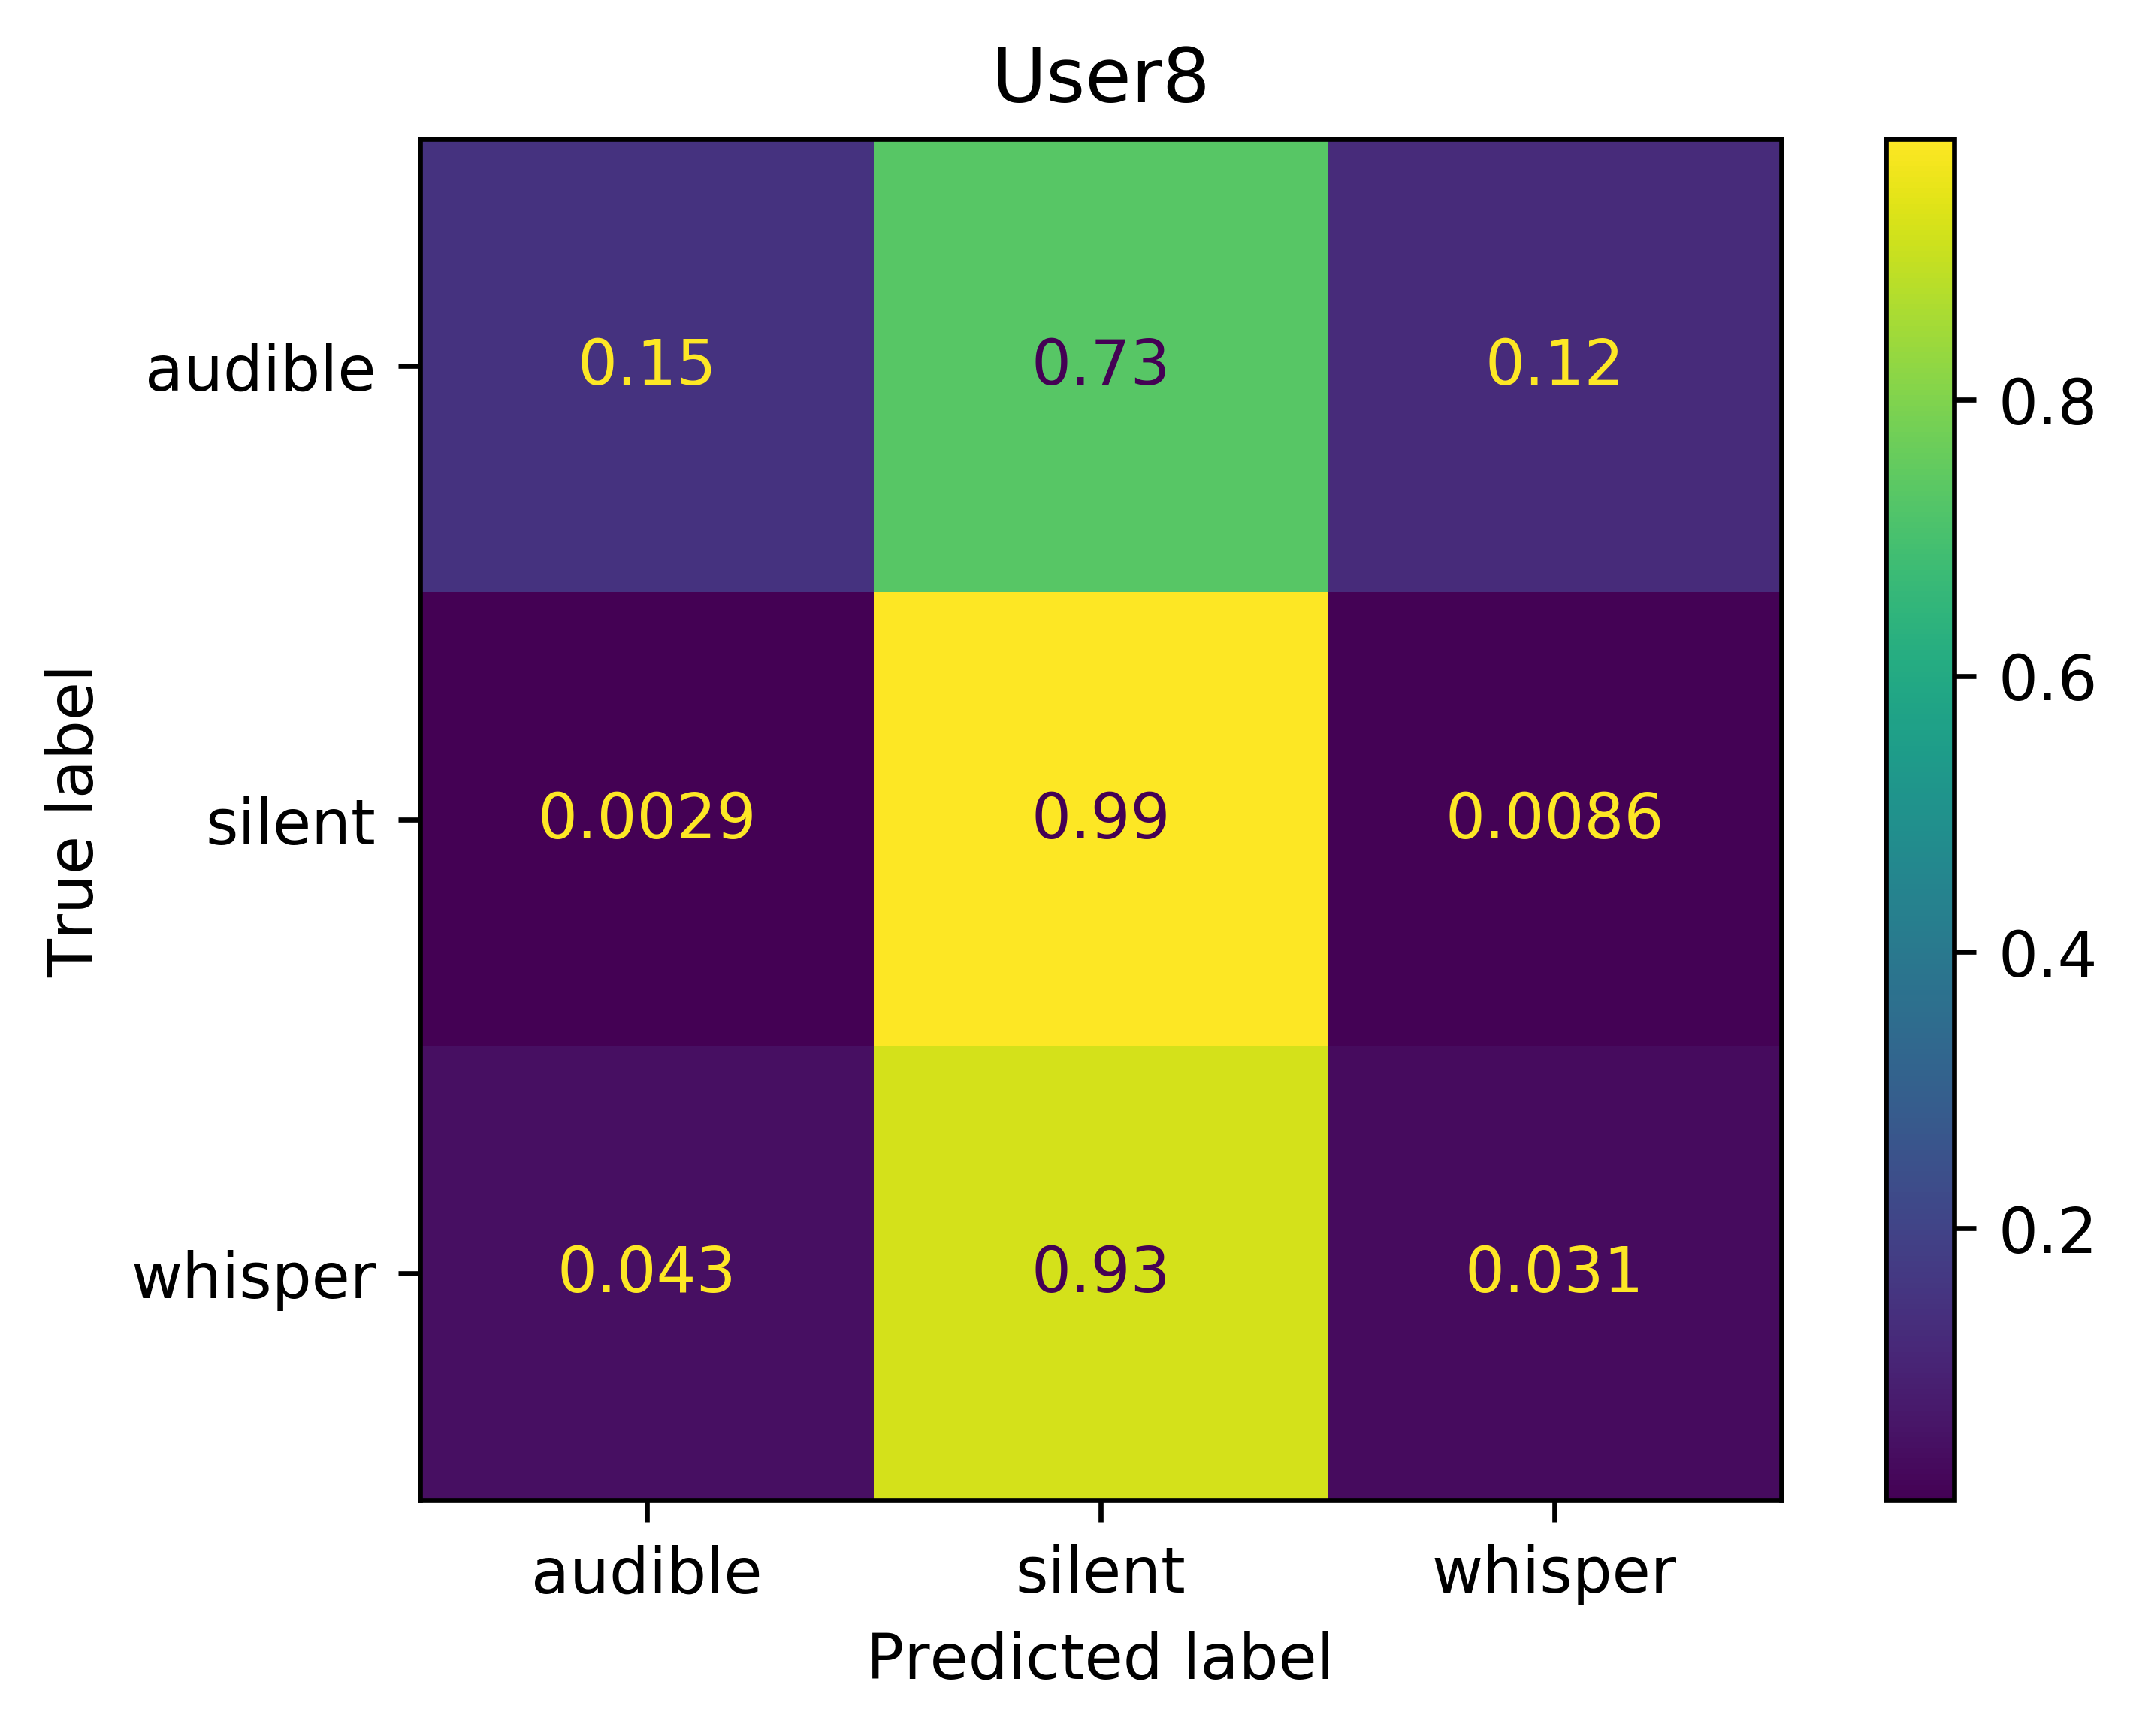
\includegraphics[width=63mm]{modeCrossUser/User8.png}}
\caption{Die Erkennungsraten der Sprecher  für die Vorhersage des Sprachmodus mit gefilterten Daten.}
\label{fig:cnfsfiltered}
\end{figure}


\subsubsection{Frequenzbänder}
Hier wird derselbe Versuch wie in der Cross-User Version durchgeführt. Die Resultate sind in \ref{fig:mode6} zu sehen. Es ist eine ziemlich gleichmäßige Verteilung der Genauigkeiten im 44–50 Prozent Bereich zu beobachten mit den niedrigsten Werten an den beiden Enden mit 33.1 Prozent im 290-300Hz Bereich und 36.02 Prozent im 0–10 Hz Bereich. Der höchste Wert ist im 120-130Hz Bereich mit 50.41 Prozent zu beobachten. Es lässt sich eine höhere durchschnittliche Genauigkeit in den Frequenzbereichen um 190-290Hz beobachten. Aufgrund der nur sehr kleine Unterschiede zwischen den verschiedenen Frequenzbändern lässt sich allerdings kein Frequenzbereich eingrenzen, in dem die Resultate signifikant höher sind.

 \begin{figure}[H]
  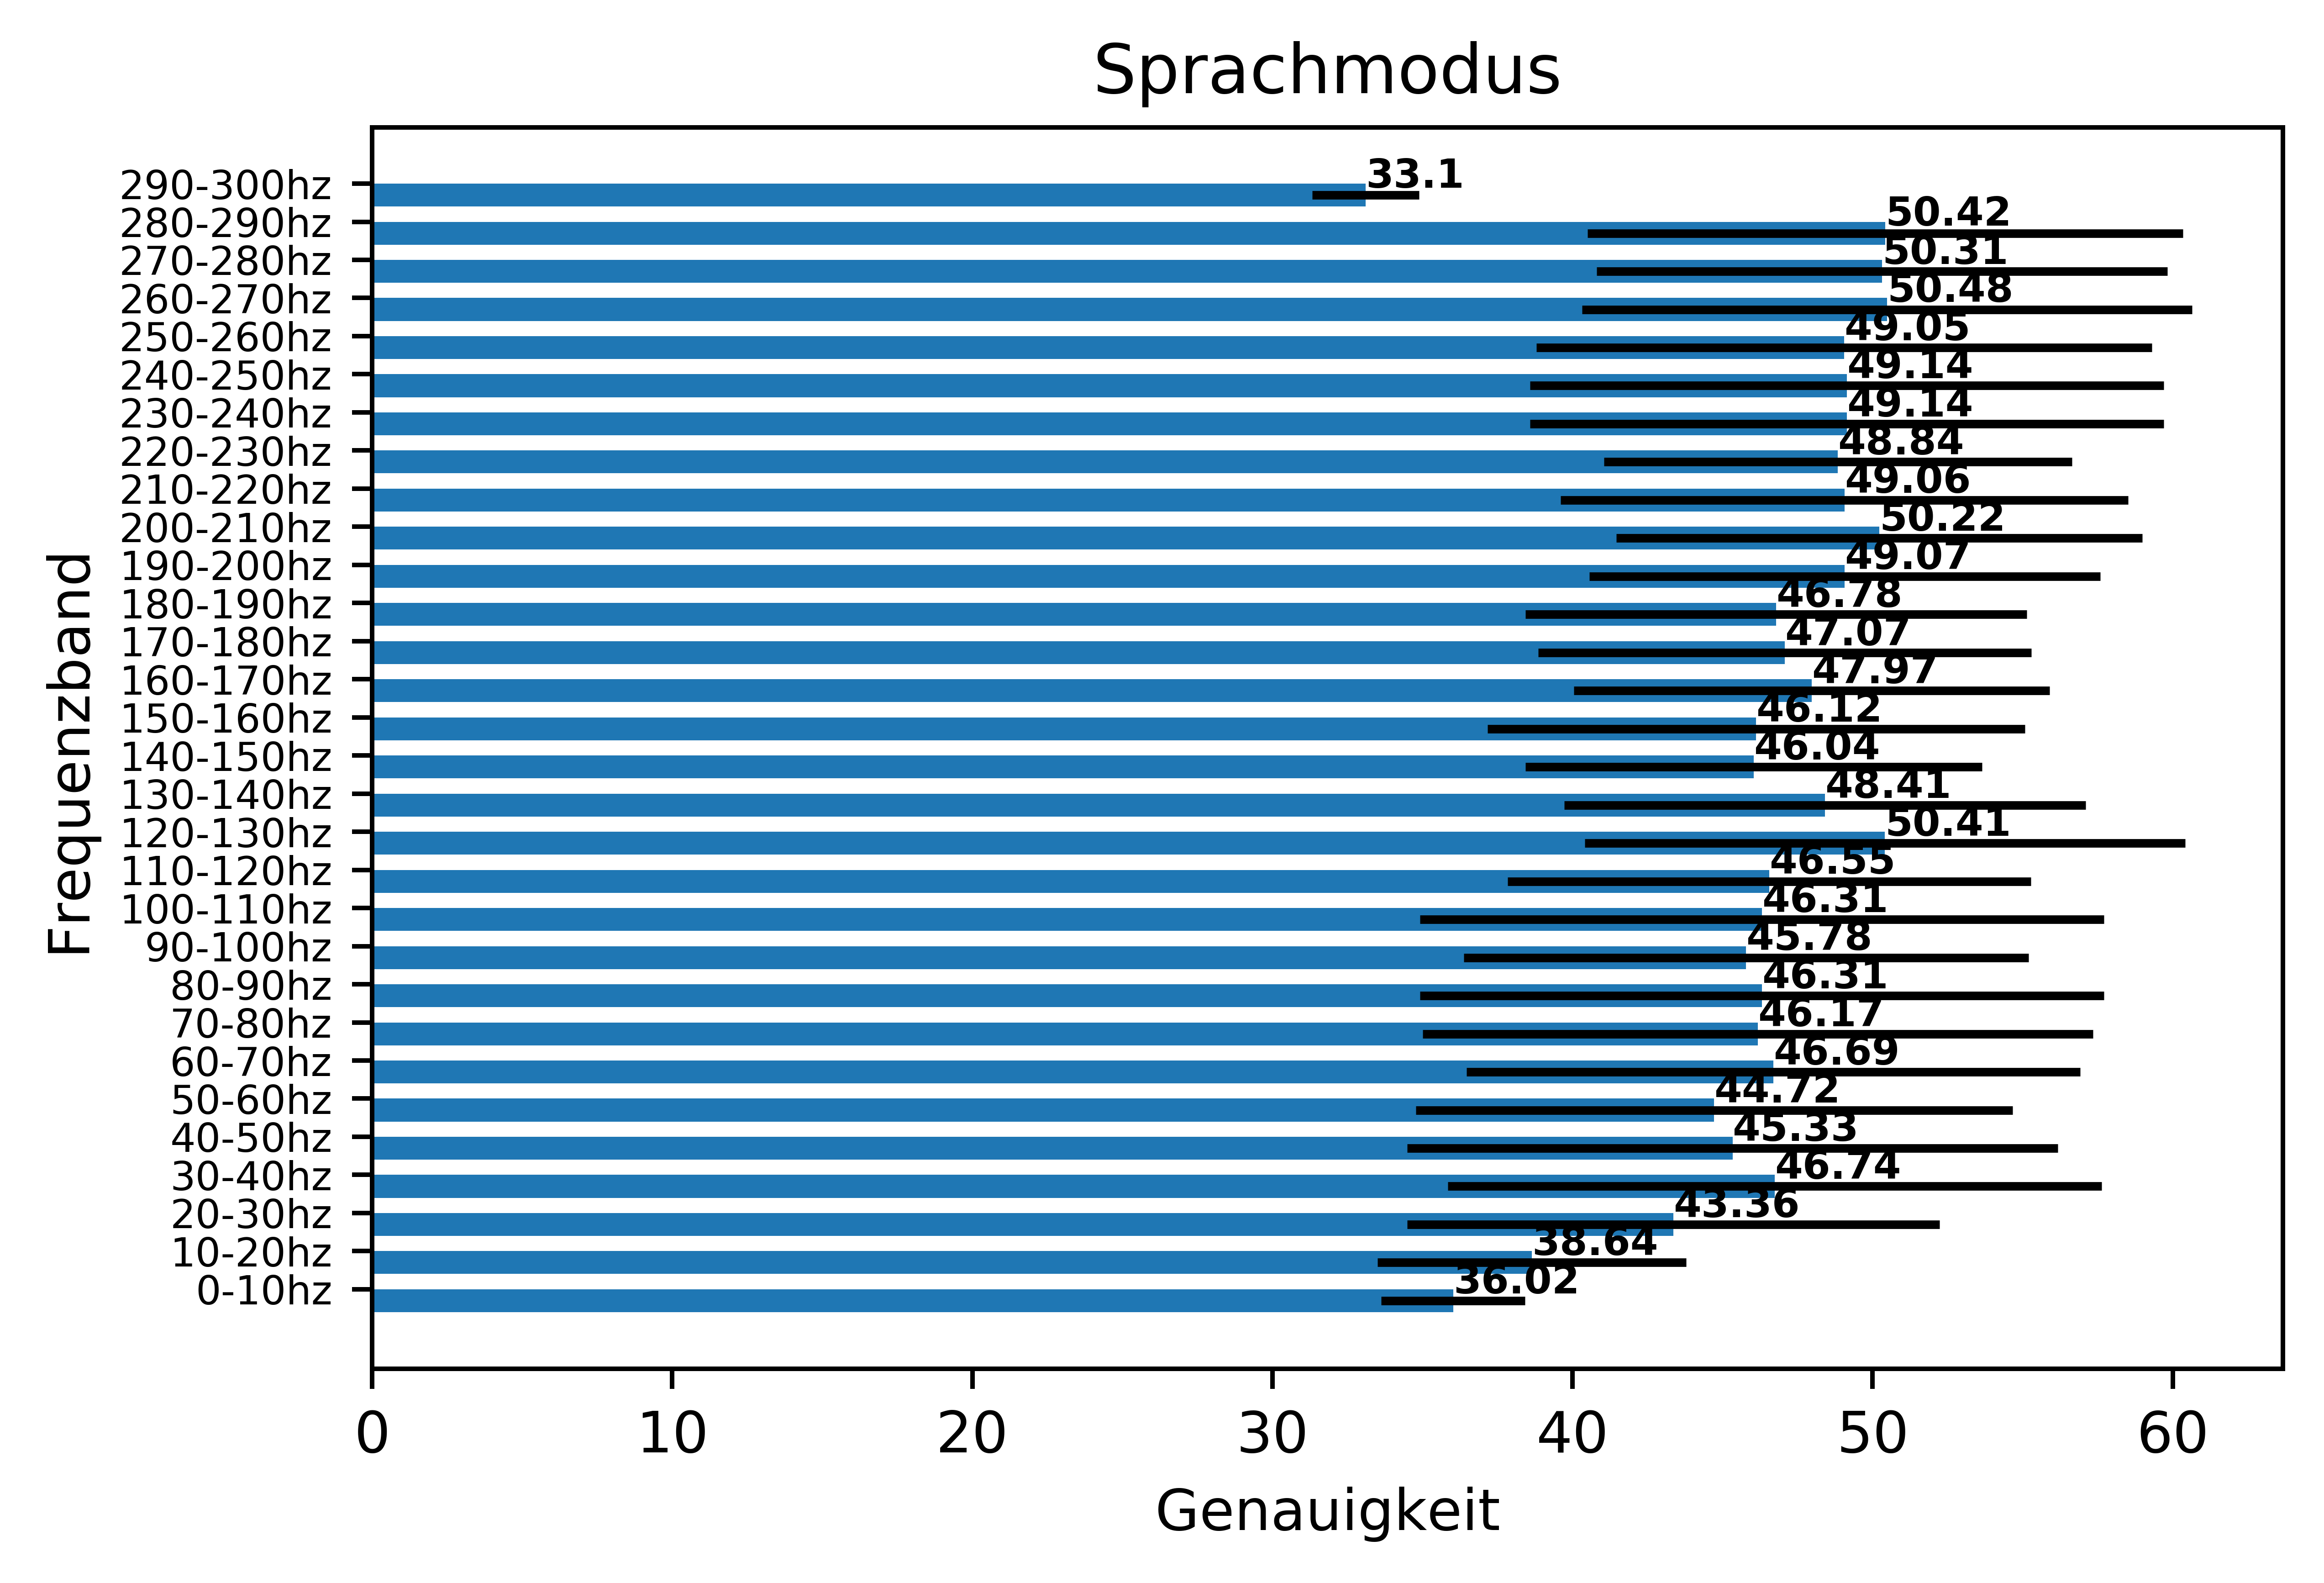
\includegraphics[width=\linewidth]{hqFreBandResultsUser.png}
  \caption{Die durchschnittliche Genauigkeit, sowie die Standardabweichung der verschiedenen Frequenzbänder.Hier werden die Daten aller Sprecher verwendet die mindestens 2 Sessions besitzen, also die Sprecher 1,2,4,7 und 8. Es handelt sich um Frequenzbänder 0-300hz in 10hz Schritten. Hier wird die Cross-User Aufteilung verwendet.}
  \label{fig:mode6}
  \end{figure}